\documentclass[10pt]{article}
\usepackage[a4paper,landscape,margin=1.4cm]{geometry}
\usepackage{amsmath,amssymb}
\usepackage{graphicx,booktabs,longtable,array,float,caption}
\usepackage[hidelinks]{hyperref}
\captionsetup{font=small,labelfont=bf}
\setlength{\parskip}{3pt}
\graphicspath{{../dist/}}
\begin{document}
\begin{center}{\LARGE\bfseries Fluid nerve atlas}\\[4pt]
{\large 106 systems: 35 atom-based (heavy-atom sites), 36 backbone-based (C$\alpha$ sites), 35 paired heavy-atom representations}\\[3pt]
Joseph Campagna, PSM --- pronerv fluid-nerve pipeline --- \today\end{center}

\section*{How to read the plates}
Every plate shows one system in six panels. \textbf{(A)} the biophysical object: the recorded conformation nearest the occupancy
peak of the chart, drawn from its sites (heavy atoms with element colours, or the C$\alpha$ trace coloured from the N- to the C-terminus),
with the deformation field drawn on the molecule as arrows: the mean rigid-aligned displacement of every site over the reference lag,
conditional on the chart bin of that conformation. \textbf{(B)} the chart (backbone dihedrals on a torus, or the two leading principal
components of the aligned sites) with the occupancy, the 18 cover balls and the drawn nerve; one composable pair is annotated in the
language of the legend below. \textbf{(C)} the deformation field on the chart: mobility $h$ (colour) and drift $v$ (arrows).
\textbf{(D)} the fluid filtration: Betti numbers of the nerve of the cover thickened by $\pm\tau$ frames along each run.
\textbf{(E)} the flooding filtration of the occupancy landscape (sublevel sets of $-\log p$), the geometric analogue of metadynamics.
\textbf{(F)} the categorical reading: the sizes of the category drawn in (B), the Betti numbers of the witnessed complex, the
ambient-time invariants and the field summaries. All constructions are descriptive: no equilibrium free energy, rate constant or
configuration-space nerve theorem is claimed.

\begin{figure}[H]\centering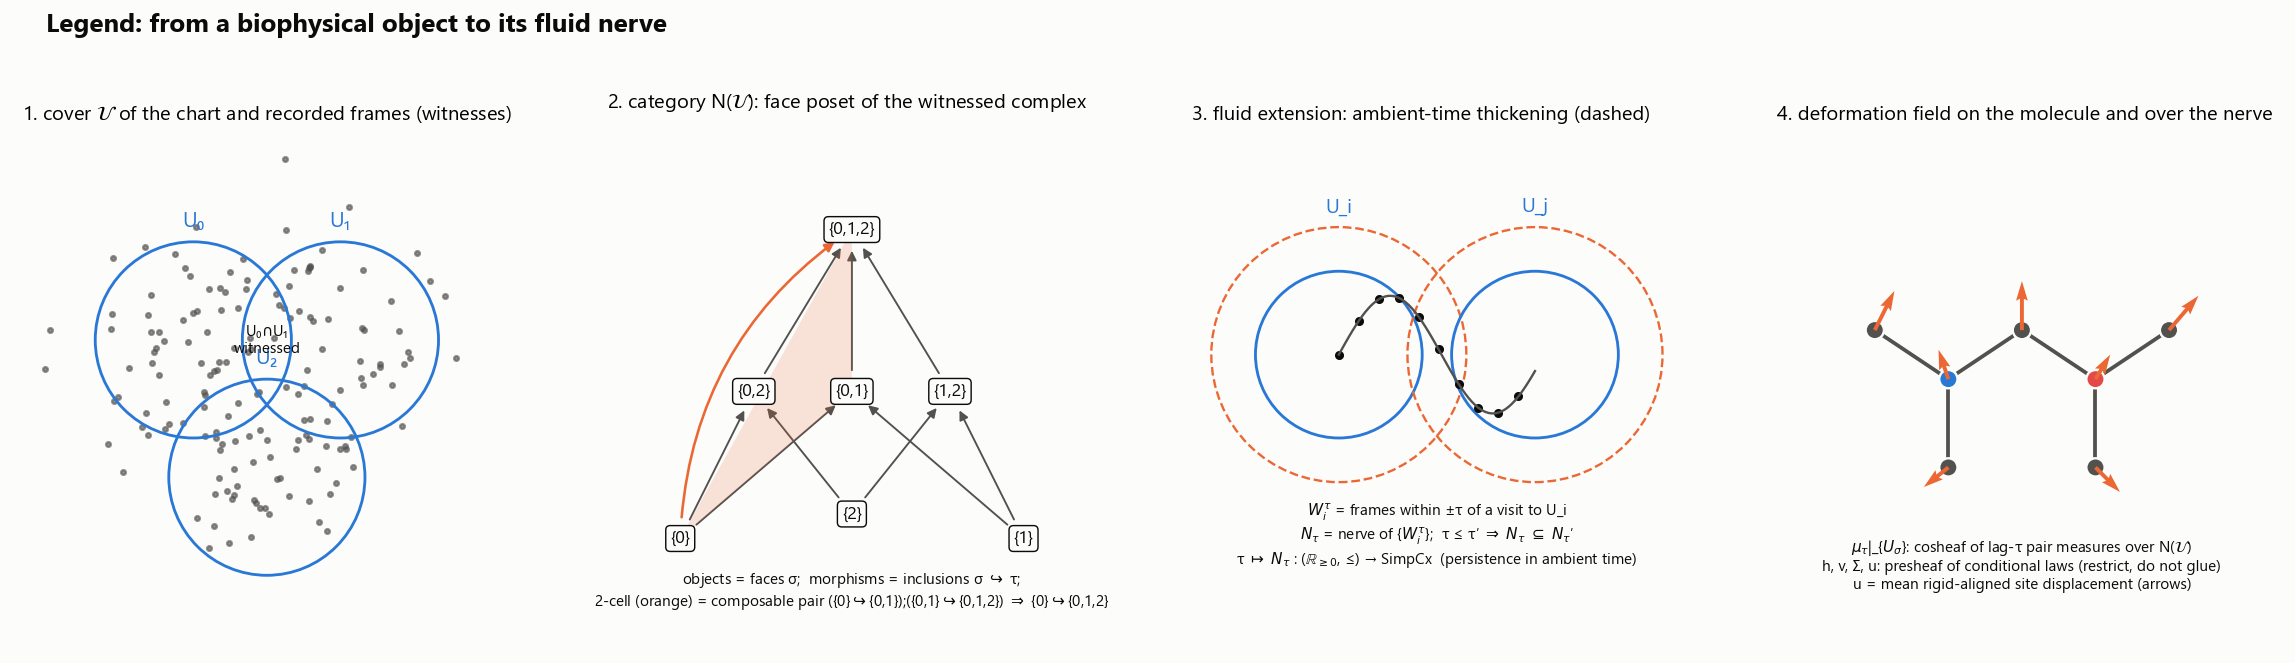
\includegraphics[width=\linewidth]{comparison/fig_legend.png}
\caption{\textbf{Legend in categorical terms.} (1) A cover $\mathcal U=\{U_i\}$ of the chart; the recorded frames are the witnesses.
(2) The witnessed complex $K(\mathcal U;S)$ and its face poset $N(\mathcal U)$ seen as a category: \emph{objects} are faces $\sigma$ (the witnessed intersections $U_\sigma=\bigcap_{i\in\sigma}U_i$),
\emph{morphisms} are inclusions $\sigma\hookrightarrow\tau$ with composition given by transitivity and implicit identities, \emph{2-cells} are composable pairs
$(\sigma\hookrightarrow\tau);(\tau\hookrightarrow\rho)\Rightarrow\sigma\hookrightarrow\rho$ (Street's orientals; exported to homotopy.io together with the 3-cells of length-three chains and of quadruple overlaps).
(3) The \emph{fluid extension}: thickening every cover set by $\pm\tau$ frames along the recorded runs gives $W_i^\tau$ and the nerve $N_\tau$;
$\tau\mapsto N_\tau$ is a functor from the poset $(\mathbb R_{\ge0},\le)$ to simplicial complexes, whose homology is a persistence module in ambient time.
(4) The \emph{deformation field}: the lag-$\tau$ pair measure $\mu_\tau$ restricted to the objects $U_\sigma$ is a cosheaf over $N(\mathcal U)$; the derived
statistics (mobility $h$, drift $v$, spread $\Sigma$, site displacement $u$) form a presheaf of conditional laws, drawn on the molecule in panel (A) and on the chart in panel (C).
The theory PDF (\texttt{fluid-nerve-theory.pdf}) proves that nerves of formally open covers are rigid under infinitesimal transformations, so the ambient-time behaviour seen in (D) is a finite-time, finite-witness phenomenon.}
\end{figure}
\clearpage
\section*{Catalog}
\begin{small}\begin{longtable}{p{3.9cm}p{5.2cm}llrrrlrlr}
\caption{All systems. Nerve counts are objects/morphisms/2-cells of the drawn face-poset nerve; $\beta$ are GF(2) Betti numbers of the witnessed complex; $h$ the median supported mobility at the reference lag; $\tau_{\mathrm c}$ the ambient-time connection; $r_{\mathrm c}$ the cover-radius factor at which $\beta_0=1$.}\\
\toprule id & system & group & repr. & sites & frames & runs & nerve & $\beta_{0,1,2}$ & $\tau_{\mathrm c}$ & $h$ (nm)\\\midrule\endfirsthead
\toprule id & system & group & repr. & sites & frames & runs & nerve & $\beta_{0,1,2}$ & $\tau_{\mathrm c}$ & $h$ (nm)\\\midrule\endhead
dipeptide-ala & Ace-ALA-NMe dipeptide (OpenMM) & atom & heavy & 10 & 30,000 & 3 & 196/792/654 & 1,0,0 & 0 fs & 0.0416\\
dipeptide-arg & Ace-ARG-NMe dipeptide (OpenMM) & atom & heavy & 16 & 30,000 & 3 & 133/486/384 & 2,0,0 & 1 ps & 0.0717\\
dipeptide-asn & Ace-ASN-NMe dipeptide (OpenMM) & atom & heavy & 13 & 30,000 & 3 & 289/1278/1104 & 1,0,0 & 0 fs & 0.0568\\
dipeptide-asp & Ace-ASP-NMe dipeptide (OpenMM) & atom & heavy & 13 & 30,000 & 3 & 213/878/732 & 1,0,0 & 0 fs & 0.0538\\
dipeptide-cys & Ace-CYS-NMe dipeptide (OpenMM) & atom & heavy & 11 & 30,000 & 3 & 255/1106/948 & 1,0,0 & 0 fs & 0.0408\\
dipeptide-gln & Ace-GLN-NMe dipeptide (OpenMM) & atom & heavy & 14 & 30,000 & 3 & 236/1000/846 & 1,0,0 & 0 fs & 0.0631\\
dipeptide-glu & Ace-GLU-NMe dipeptide (OpenMM) & atom & heavy & 14 & 30,000 & 3 & 235/994/840 & 1,0,0 & 0 fs & 0.0653\\
dipeptide-gly & Ace-GLY-NMe dipeptide (OpenMM) & atom & heavy & 9 & 30,000 & 3 & 87/246/162 & 1,4,0 & 0 fs & 0.0461\\
dipeptide-his & Ace-HIS-NMe dipeptide (OpenMM) & atom & heavy & 15 & 30,000 & 3 & 230/972/822 & 1,0,0 & 0 fs & 0.055\\
dipeptide-ile & Ace-ILE-NMe dipeptide (OpenMM) & atom & heavy & 13 & 30,000 & 3 & 262/1148/990 & 1,0,0 & 0 fs & 0.0361\\
dipeptide-leu & Ace-LEU-NMe dipeptide (OpenMM) & atom & heavy & 13 & 30,000 & 3 & 270/1180/1014 & 1,0,0 & 0 fs & 0.0457\\
dipeptide-lys & Ace-LYS-NMe dipeptide (OpenMM) & atom & heavy & 14 & 30,000 & 3 & 179/722/600 & 2,0,0 & 1 ps & 0.0568\\
dipeptide-met & Ace-MET-NMe dipeptide (OpenMM) & atom & heavy & 13 & 30,000 & 3 & 232/972/816 & 1,0,0 & 0 fs & 0.0573\\
dipeptide-phe & Ace-PHE-NMe dipeptide (OpenMM) & atom & heavy & 16 & 30,000 & 3 & 261/1138/978 & 1,0,0 & 0 fs & 0.0468\\
dipeptide-pro & Ace-PRO-NMe dipeptide (OpenMM) & atom & heavy & 12 & 30,000 & 3 & 258/1152/1008 & 2,0,0 & 1 ps & 0.0187\\
dipeptide-ser & Ace-SER-NMe dipeptide (OpenMM) & atom & heavy & 11 & 30,000 & 3 & 185/734/600 & 1,0,0 & 0 fs & 0.0408\\
dipeptide-thr & Ace-THR-NMe dipeptide (OpenMM) & atom & heavy & 12 & 30,000 & 3 & 214/888/744 & 1,0,0 & 0 fs & 0.035\\
dipeptide-trp & Ace-TRP-NMe dipeptide (OpenMM) & atom & heavy & 19 & 30,000 & 3 & 249/1078/924 & 1,0,0 & 0 fs & 0.0466\\
dipeptide-tyr & Ace-TYR-NMe dipeptide (OpenMM) & atom & heavy & 17 & 30,000 & 3 & 272/1196/1032 & 1,0,0 & 0 fs & 0.0479\\
dipeptide-val & Ace-VAL-NMe dipeptide (OpenMM) & atom & heavy & 12 & 30,000 & 3 & 223/930/780 & 1,0,0 & 0 fs & 0.0336\\
sgdml-md17-aspirin & aspirin (MD17 ab initio MD) & atom & heavy & 13 & 211,762 & 1 & 158/592/468 & 1,0,0 & 0 fs & 0.0198\\
sgdml-md17-azobenzene & azobenzene (MD17 ab initio MD) & atom & heavy & 14 & 99,999 & 1 & 63/146/84 & 1,1,0 & 0 fs & 0.0149\\
sgdml-md17-ethanol & ethanol (MD17 ab initio MD) & atom & heavy & 3 & 555,092 & 1 & 24/12/0 & 12,0,0 & 1.5 fs & 0.00824\\
sgdml-md17-malonaldehyde & malonaldehyde (MD17 ab initio MD) & atom & heavy & 5 & 993,237 & 1 & 79/210/132 & 1,0,0 & 0 fs & 0.0189\\
sgdml-md17-naphthalene & naphthalene (MD17 ab initio MD) & atom & heavy & 10 & 326,250 & 1 & 41/58/18 & 2,1,0 & 0.5 fs & 0.00821\\
sgdml-md17-paracetamol & paracetamol (MD17 ab initio MD) & atom & heavy & 11 & 106,490 & 1 & 72/188/120 & 1,1,0 & 0 fs & 0.0148\\
sgdml-md17-salicylic & salicylic (MD17 ab initio MD) & atom & heavy & 10 & 320,231 & 1 & 25/14/0 & 11,0,0 & 11 fs & 0.0097\\
sgdml-md17-toluene & toluene (MD17 ab initio MD) & atom & heavy & 7 & 442,790 & 1 & 28/20/0 & 8,0,0 & 1.5 fs & 0.00765\\
sgdml-md17-uracil & uracil (MD17 ab initio MD) & atom & heavy & 8 & 133,770 & 1 & 31/34/12 & 9,0,0 & 8.5 fs & 0.00852\\
sgdml-md22-ac-ala3-nhme & Ac-Ala3-NHMe (MD22 ab initio MD) & atom & heavy & 20 & 85,109 & 1 & 64/140/72 & 1,6,0 & 0 fs & 0.0276\\
sgdml-md22-at-at & AT-AT (MD22 ab initio MD) & atom & heavy & 38 & 20,001 & 1 & 118/412/318 & 1,0,0 & 0 fs & --\\
sgdml-md22-at-at-cg-cg & AT-AT-CG-CG (MD22 ab initio MD) & atom & heavy & 76 & 10,153 & 1 & 135/490/384 & 1,0,0 & 0 fs & --\\
sgdml-md22-dha & DHA (MD22 ab initio MD) & atom & heavy & 24 & 69,753 & 1 & 88/248/162 & 1,3,0 & 0 fs & 0.0339\\
sgdml-md22-stachyose & stachyose (MD22 ab initio MD) & atom & heavy & 45 & 27,272 & 1 & 144/536/426 & 1,0,0 & 0 fs & --\\
ala2 & Alanine dipeptide (mdshare) & atom & heavy & 10 & 750,000 & 3 & 78/212/138 & 3,3,0 & 1 ps & 0.0383\\
cln025 & Chignolin CLN025 (128-run subset) & backbone & C$\alpha$ & 10 & 63,999 & 128 & 84/228/144 & 1,2,0 & 0 fr & 0.197\\
mdcath-1a92a00-ca & CATH domain 1a92A00 (mdCATH), C-alpha & backbone & C$\alpha$ & 50 & 10,980 & 25 & 89/254/168 & 1,0,0 & 0 fs & 0.697\\
mdcath-1b33n01-ca & CATH domain 1b33N01 (mdCATH), C-alpha & backbone & C$\alpha$ & 55 & 11,090 & 25 & 80/216/138 & 2,3,0 & 1 ns & 0.316\\
mdcath-1bdha01-ca & CATH domain 1bdhA01 (mdCATH), C-alpha & backbone & C$\alpha$ & 57 & 11,110 & 25 & 76/196/120 & 1,1,0 & 0 fs & 0.635\\
mdcath-1e5wa04-ca & CATH domain 1e5wA04 (mdCATH), C-alpha & backbone & C$\alpha$ & 55 & 10,910 & 25 & 96/288/198 & 1,1,0 & 0 fs & 0.848\\
mdcath-1ffsb00-ca & CATH domain 1ffsB00 (mdCATH), C-alpha & backbone & C$\alpha$ & 68 & 11,141 & 25 & 139/510/402 & 2,0,0 & 1 ns & 0.419\\
mdcath-1gjsa00-ca & CATH domain 1gjsA00 (mdCATH), C-alpha & backbone & C$\alpha$ & 65 & 10,970 & 25 & 86/244/162 & 1,1,0 & 0 fs & 0.604\\
mdcath-1ha8a00-ca & CATH domain 1ha8A00 (mdCATH), C-alpha & backbone & C$\alpha$ & 51 & 11,150 & 25 & 78/208/132 & 1,1,0 & 0 fs & 0.21\\
mdcath-1hcra00-ca & CATH domain 1hcrA00 (mdCATH), C-alpha & backbone & C$\alpha$ & 52 & 11,160 & 25 & 65/146/78 & 1,4,0 & 0 fs & 0.691\\
mdcath-1i5xa00-ca & CATH domain 1i5xA00 (mdCATH), C-alpha & backbone & C$\alpha$ & 61 & 11,080 & 25 & 106/336/240 & 1,0,0 & 0 fs & 0.606\\
mdcath-1ib8a02-ca & CATH domain 1ib8A02 (mdCATH), C-alpha & backbone & C$\alpha$ & 67 & 11,090 & 25 & 86/244/162 & 1,2,0 & 0 fs & 0.409\\
mdcath-1klil00-ca & CATH domain 1kliL00 (mdCATH), C-alpha & backbone & C$\alpha$ & 61 & 11,100 & 25 & 80/216/138 & 1,1,0 & 0 fs & 0.552\\
mdcath-1l6ha00-ca & CATH domain 1l6hA00 (mdCATH), C-alpha & backbone & C$\alpha$ & 69 & 11,090 & 25 & 77/198/120 & 1,2,0 & 0 fs & 0.344\\
mdcath-1r8ob01-ca & CATH domain 1r8oB01 (mdCATH), C-alpha & backbone & C$\alpha$ & 66 & 11,100 & 25 & 87/246/162 & 1,1,0 & 0 fs & 0.908\\
mdcath-1s6la01-ca & CATH domain 1s6lA01 (mdCATH), C-alpha & backbone & C$\alpha$ & 52 & 11,170 & 25 & 100/308/216 & 1,0,0 & 0 fs & 0.685\\
mdcath-1v1hf01-ca & CATH domain 1v1hF01 (mdCATH), C-alpha & backbone & C$\alpha$ & 73 & 10,806 & 25 & 99/306/216 & 1,0,0 & 0 fs & 0.788\\
mdcath-1wfwa00-ca & CATH domain 1wfwA00 (mdCATH), C-alpha & backbone & C$\alpha$ & 74 & 11,190 & 25 & 72/176/102 & 1,4,0 & 0 fs & 0.347\\
mdcath-1wpbg01-ca & CATH domain 1wpbG01 (mdCATH), C-alpha & backbone & C$\alpha$ & 54 & 10,980 & 25 & 102/320/228 & 1,0,0 & 0 fs & 0.549\\
mdcath-1x4pa00-ca & CATH domain 1x4pA00 (mdCATH), C-alpha & backbone & C$\alpha$ & 66 & 11,130 & 25 & 76/196/120 & 1,2,0 & 0 fs & 0.799\\
mdcath-1zbqa02-ca & CATH domain 1zbqA02 (mdCATH), C-alpha & backbone & C$\alpha$ & 58 & 11,190 & 25 & 81/218/138 & 1,3,0 & 0 fs & 0.799\\
mdcath-2ckka02-ca & CATH domain 2ckkA02 (mdCATH), C-alpha & backbone & C$\alpha$ & 57 & 12,500 & 25 & 118/392/288 & 1,1,0 & 0 fs & 0.239\\
mdcath-2d46a00-ca & CATH domain 2d46A00 (mdCATH), C-alpha & backbone & C$\alpha$ & 61 & 11,390 & 25 & 90/260/174 & 1,0,0 & 0 fs & 1.02\\
mdcath-2dmpa01-ca & CATH domain 2dmpA01 (mdCATH), C-alpha & backbone & C$\alpha$ & 55 & 12,500 & 25 & 76/196/120 & 1,2,0 & 0 fs & 0.886\\
mdcath-2e3tb03-ca & CATH domain 2e3tB03 (mdCATH), C-alpha & backbone & C$\alpha$ & 61 & 11,390 & 25 & 116/384/282 & 1,0,0 & 0 fs & 0.489\\
mdcath-2j8ga03-ca & CATH domain 2j8gA03 (mdCATH), C-alpha & backbone & C$\alpha$ & 58 & 12,130 & 25 & 91/266/180 & 1,0,0 & 0 fs & 0.732\\
mdcath-2jrra01-ca & CATH domain 2jrrA01 (mdCATH), C-alpha & backbone & C$\alpha$ & 53 & 12,500 & 25 & 93/282/198 & 1,0,0 & 0 fs & 0.292\\
mdcath-2kssa01-ca & CATH domain 2kssA01 (mdCATH), C-alpha & backbone & C$\alpha$ & 63 & 12,500 & 25 & 50/92/42 & 2,2,0 & 1 ns & 0.764\\
mdcath-2lrda00-ca & CATH domain 2lrdA00 (mdCATH), C-alpha & backbone & C$\alpha$ & 61 & 12,500 & 25 & 74/188/114 & 1,2,0 & 0 fs & 0.21\\
mdcath-2xepa03-ca & CATH domain 2xepA03 (mdCATH), C-alpha & backbone & C$\alpha$ & 53 & 11,390 & 25 & 77/198/120 & 1,4,0 & 0 fs & 0.6\\
mdcath-2yila02-ca & CATH domain 2yilA02 (mdCATH), C-alpha & backbone & C$\alpha$ & 51 & 12,500 & 25 & 96/300/216 & 1,0,0 & 0 fs & 0.247\\
mdcath-3g5ca02-ca & CATH domain 3g5cA02 (mdCATH), C-alpha & backbone & C$\alpha$ & 55 & 12,500 & 25 & 85/238/156 & 1,0,0 & 0 fs & 0.476\\
mdcath-3pmqa02-ca & CATH domain 3pmqA02 (mdCATH), C-alpha & backbone & C$\alpha$ & 50 & 12,130 & 25 & 68/160/90 & 1,4,0 & 0 fs & 0.872\\
mdcath-4a0ta01-ca & CATH domain 4a0tA01 (mdCATH), C-alpha & backbone & C$\alpha$ & 61 & 11,390 & 25 & 75/190/114 & 1,3,0 & 0 fs & 0.688\\
mdcath-4dcza00-ca & CATH domain 4dczA00 (mdCATH), C-alpha & backbone & C$\alpha$ & 55 & 11,020 & 25 & 81/218/138 & 1,1,0 & 0 fs & 0.777\\
mdcath-5b1aj00-ca & CATH domain 5b1aJ00 (mdCATH), C-alpha & backbone & C$\alpha$ & 58 & 11,950 & 25 & 76/196/120 & 1,3,0 & 0 fs & 0.58\\
mdcath-5daea00-ca & CATH domain 5daeA00 (mdCATH), C-alpha & backbone & C$\alpha$ & 57 & 11,390 & 25 & 72/172/96 & 1,5,0 & 0 fs & 0.281\\
mdcath-1a92a00-heavy & CATH domain 1a92A00 (mdCATH), heavy atoms & paired & heavy & 427 & 10,980 & 25 & 102/316/222 & 1,1,0 & 0 fs & 0.669\\
mdcath-1b33n01-heavy & CATH domain 1b33N01 (mdCATH), heavy atoms & paired & heavy & 471 & 11,090 & 25 & 68/156/84 & 1,6,0 & 0 fs & 0.47\\
mdcath-1bdha01-heavy & CATH domain 1bdhA01 (mdCATH), heavy atoms & paired & heavy & 446 & 11,110 & 25 & 77/202/126 & 1,0,0 & 0 fs & 0.623\\
mdcath-1e5wa04-heavy & CATH domain 1e5wA04 (mdCATH), heavy atoms & paired & heavy & 483 & 10,910 & 25 & 96/288/198 & 1,0,0 & 0 fs & 0.913\\
mdcath-1ffsb00-heavy & CATH domain 1ffsB00 (mdCATH), heavy atoms & paired & heavy & 518 & 11,141 & 25 & 128/456/354 & 2,0,0 & 1 ns & 0.698\\
mdcath-1gjsa00-heavy & CATH domain 1gjsA00 (mdCATH), heavy atoms & paired & heavy & 504 & 10,970 & 25 & 99/302/210 & 1,1,0 & 0 fs & 0.648\\
mdcath-1ha8a00-heavy & CATH domain 1ha8A00 (mdCATH), heavy atoms & paired & heavy & 352 & 11,150 & 25 & 78/204/126 & 1,3,0 & 0 fs & 0.242\\
mdcath-1hcra00-heavy & CATH domain 1hcrA00 (mdCATH), heavy atoms & paired & heavy & 430 & 11,160 & 25 & 75/190/114 & 1,4,0 & 0 fs & 0.72\\
mdcath-1i5xa00-heavy & CATH domain 1i5xA00 (mdCATH), heavy atoms & paired & heavy & 499 & 11,080 & 25 & 94/280/192 & 1,2,0 & 0 fs & 0.665\\
mdcath-1ib8a02-heavy & CATH domain 1ib8A02 (mdCATH), heavy atoms & paired & heavy & 534 & 11,090 & 25 & 96/296/210 & 1,0,0 & 0 fs & 0.215\\
mdcath-1klil00-heavy & CATH domain 1kliL00 (mdCATH), heavy atoms & paired & heavy & 472 & 11,100 & 25 & 77/202/126 & 1,3,0 & 0 fs & 0.633\\
mdcath-1l6ha00-heavy & CATH domain 1l6hA00 (mdCATH), heavy atoms & paired & heavy & 489 & 11,090 & 25 & 94/280/192 & 1,1,0 & 0 fs & 0.401\\
mdcath-1r8ob01-heavy & CATH domain 1r8oB01 (mdCATH), heavy atoms & paired & heavy & 523 & 11,100 & 25 & 85/234/150 & 1,1,0 & 0 fs & 0.899\\
mdcath-1s6la01-heavy & CATH domain 1s6lA01 (mdCATH), heavy atoms & paired & heavy & 401 & 11,170 & 25 & 118/396/294 & 1,0,0 & 0 fs & 0.727\\
mdcath-1v1hf01-heavy & CATH domain 1v1hF01 (mdCATH), heavy atoms & paired & heavy & 532 & 10,806 & 25 & 90/260/174 & 1,1,0 & 0 fs & 0.807\\
mdcath-1wfwa00-heavy & CATH domain 1wfwA00 (mdCATH), heavy atoms & paired & heavy & 538 & 11,190 & 25 & 80/216/138 & 1,1,0 & 0 fs & 0.376\\
mdcath-1wpbg01-heavy & CATH domain 1wpbG01 (mdCATH), heavy atoms & paired & heavy & 456 & 10,980 & 25 & 102/320/228 & 1,0,0 & 0 fs & 0.638\\
mdcath-1x4pa00-heavy & CATH domain 1x4pA00 (mdCATH), heavy atoms & paired & heavy & 517 & 11,130 & 25 & 76/192/114 & 1,5,0 & 0 fs & 0.761\\
mdcath-1zbqa02-heavy & CATH domain 1zbqA02 (mdCATH), heavy atoms & paired & heavy & 466 & 11,190 & 25 & 65/146/78 & 1,4,0 & 0 fs & 0.894\\
mdcath-2ckka02-heavy & CATH domain 2ckkA02 (mdCATH), heavy atoms & paired & heavy & 438 & 12,500 & 25 & 154/560/432 & 1,0,0 & 0 fs & 0.29\\
mdcath-2d46a00-heavy & CATH domain 2d46A00 (mdCATH), heavy atoms & paired & heavy & 486 & 11,390 & 25 & 92/268/180 & 1,0,0 & 0 fs & 1.03\\
mdcath-2dmpa01-heavy & CATH domain 2dmpA01 (mdCATH), heavy atoms & paired & heavy & 470 & 12,500 & 25 & 95/282/192 & 1,0,0 & 0 fs & 0.92\\
mdcath-2e3tb03-heavy & CATH domain 2e3tB03 (mdCATH), heavy atoms & paired & heavy & 498 & 11,390 & 25 & 143/526/414 & 1,0,0 & 0 fs & 0.501\\
mdcath-2j8ga03-heavy & CATH domain 2j8gA03 (mdCATH), heavy atoms & paired & heavy & 478 & 12,130 & 25 & 70/172/102 & 2,4,0 & 1 ns & 0.834\\
mdcath-2jrra01-heavy & CATH domain 2jrrA01 (mdCATH), heavy atoms & paired & heavy & 416 & 12,500 & 25 & 123/418/312 & 1,1,0 & 0 fs & 0.312\\
mdcath-2kssa01-heavy & CATH domain 2kssA01 (mdCATH), heavy atoms & paired & heavy & 489 & 12,500 & 25 & 63/146/84 & 2,2,0 & 1 ns & 0.871\\
mdcath-2lrda00-heavy & CATH domain 2lrdA00 (mdCATH), heavy atoms & paired & heavy & 413 & 12,500 & 25 & 105/334/240 & 1,0,0 & 0 fs & 0.242\\
mdcath-2xepa03-heavy & CATH domain 2xepA03 (mdCATH), heavy atoms & paired & heavy & 424 & 11,390 & 25 & 84/232/150 & 1,3,0 & 0 fs & 0.687\\
mdcath-2yila02-heavy & CATH domain 2yilA02 (mdCATH), heavy atoms & paired & heavy & 390 & 12,500 & 25 & 73/190/120 & 1,0,0 & 0 fs & 0.336\\
mdcath-3g5ca02-heavy & CATH domain 3g5cA02 (mdCATH), heavy atoms & paired & heavy & 409 & 12,500 & 25 & 78/204/126 & 1,2,0 & 0 fs & 0.514\\
mdcath-3pmqa02-heavy & CATH domain 3pmqA02 (mdCATH), heavy atoms & paired & heavy & 385 & 12,130 & 25 & 72/176/102 & 1,4,0 & 0 fs & 0.964\\
mdcath-4a0ta01-heavy & CATH domain 4a0tA01 (mdCATH), heavy atoms & paired & heavy & 490 & 11,390 & 25 & 91/266/180 & 1,1,0 & 0 fs & 0.712\\
mdcath-4dcza00-heavy & CATH domain 4dczA00 (mdCATH), heavy atoms & paired & heavy & 466 & 11,020 & 25 & 84/236/156 & 1,0,0 & 0 fs & 0.865\\
mdcath-5b1aj00-heavy & CATH domain 5b1aJ00 (mdCATH), heavy atoms & paired & heavy & 465 & 11,950 & 25 & 86/244/162 & 1,1,0 & 0 fs & 0.641\\
mdcath-5daea00-heavy & CATH domain 5daeA00 (mdCATH), heavy atoms & paired & heavy & 438 & 11,390 & 25 & 80/216/138 & 1,2,0 & 0 fs & 0.329\\
\bottomrule\end{longtable}\end{small}\clearpage
\section*{Overview figures}
\begin{figure}[H]\centering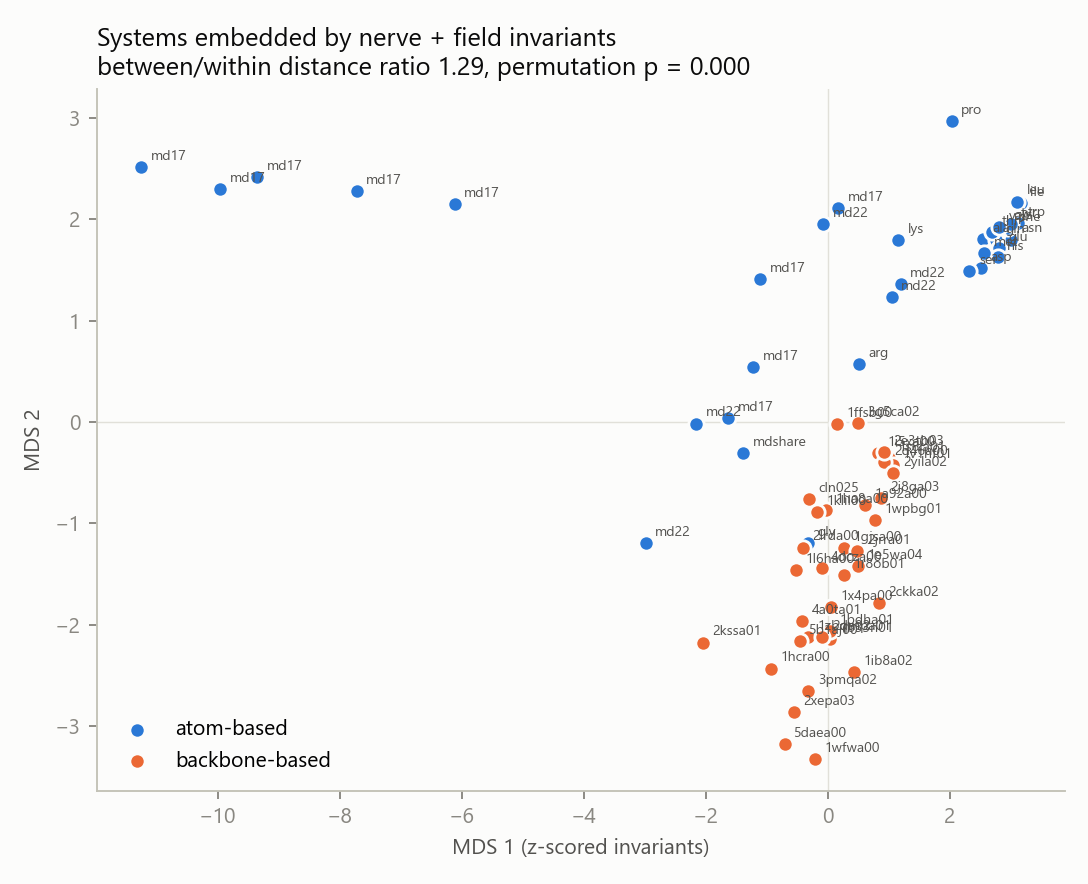
\includegraphics[width=.8\linewidth,height=.82\textheight,keepaspectratio]{comparison/fig_embedding.png}\caption{Systems embedded by nerve and field invariants (classical MDS of z-scored invariants).}\end{figure}\clearpage
\begin{figure}[H]\centering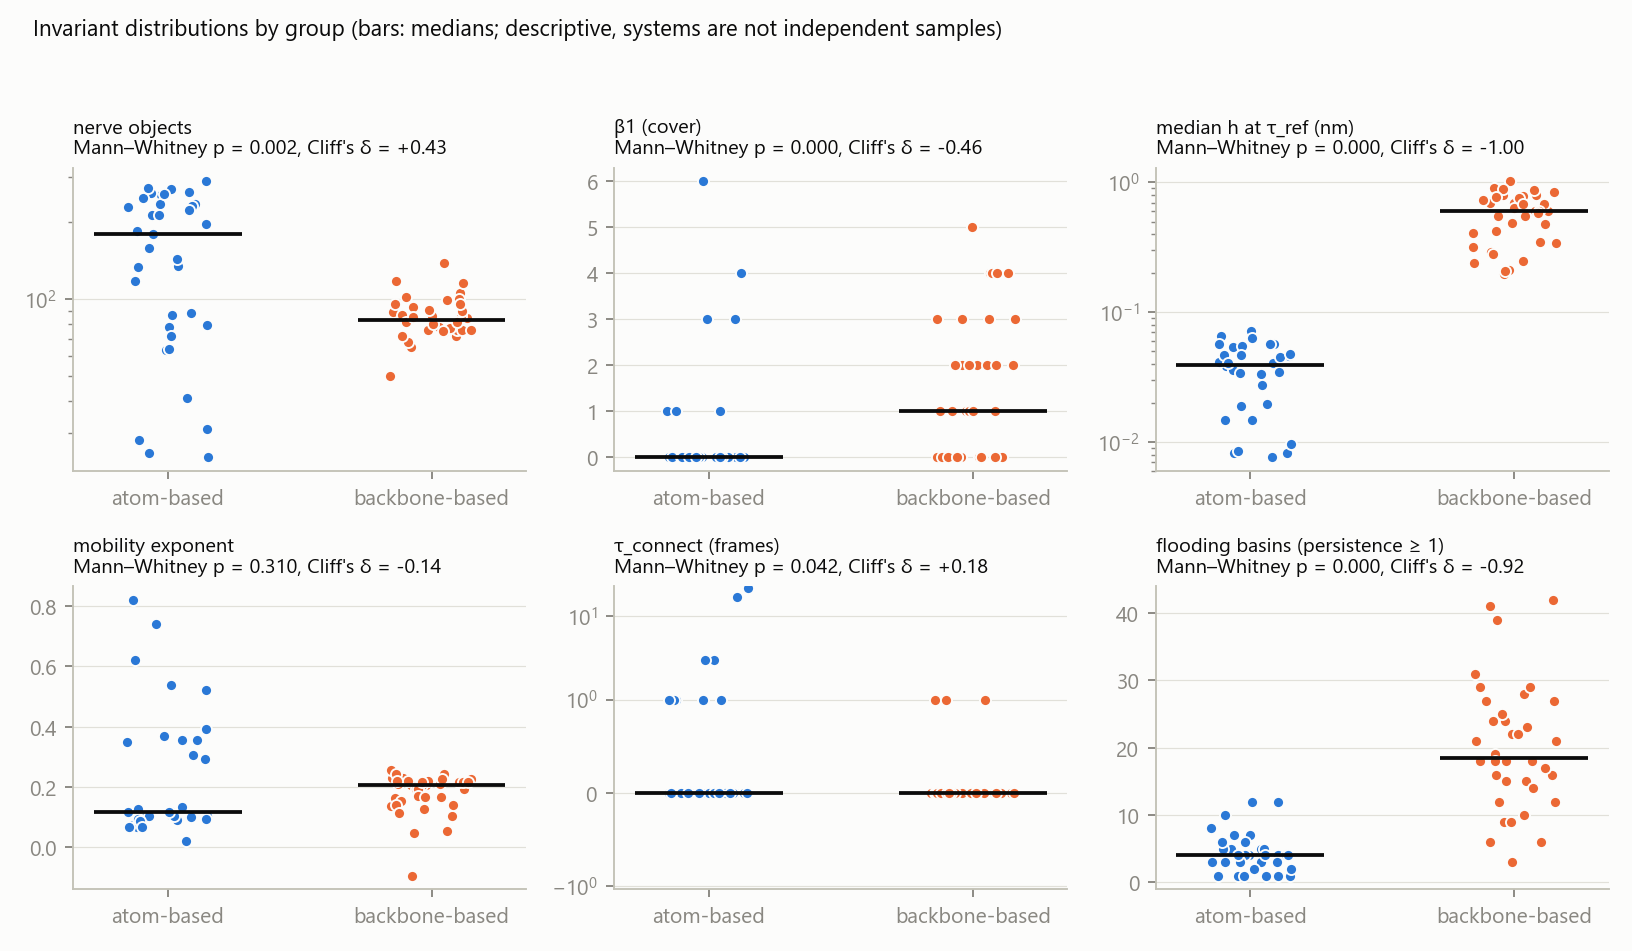
\includegraphics[width=.8\linewidth,height=.82\textheight,keepaspectratio]{comparison/fig_invariants.png}\caption{Invariant distributions by group with descriptive tests.}\end{figure}\clearpage
\begin{figure}[H]\centering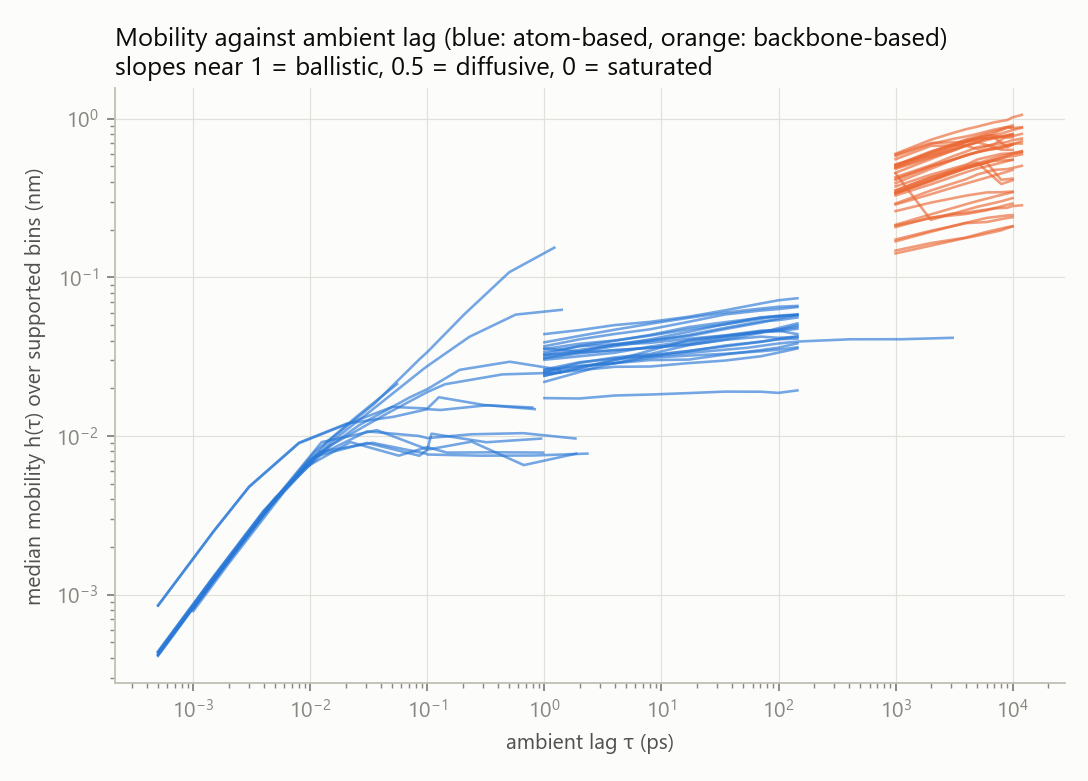
\includegraphics[width=.8\linewidth,height=.82\textheight,keepaspectratio]{comparison/fig_scaling.png}\caption{Median mobility against ambient lag; the slope is the mobility exponent.}\end{figure}\clearpage
\begin{figure}[H]\centering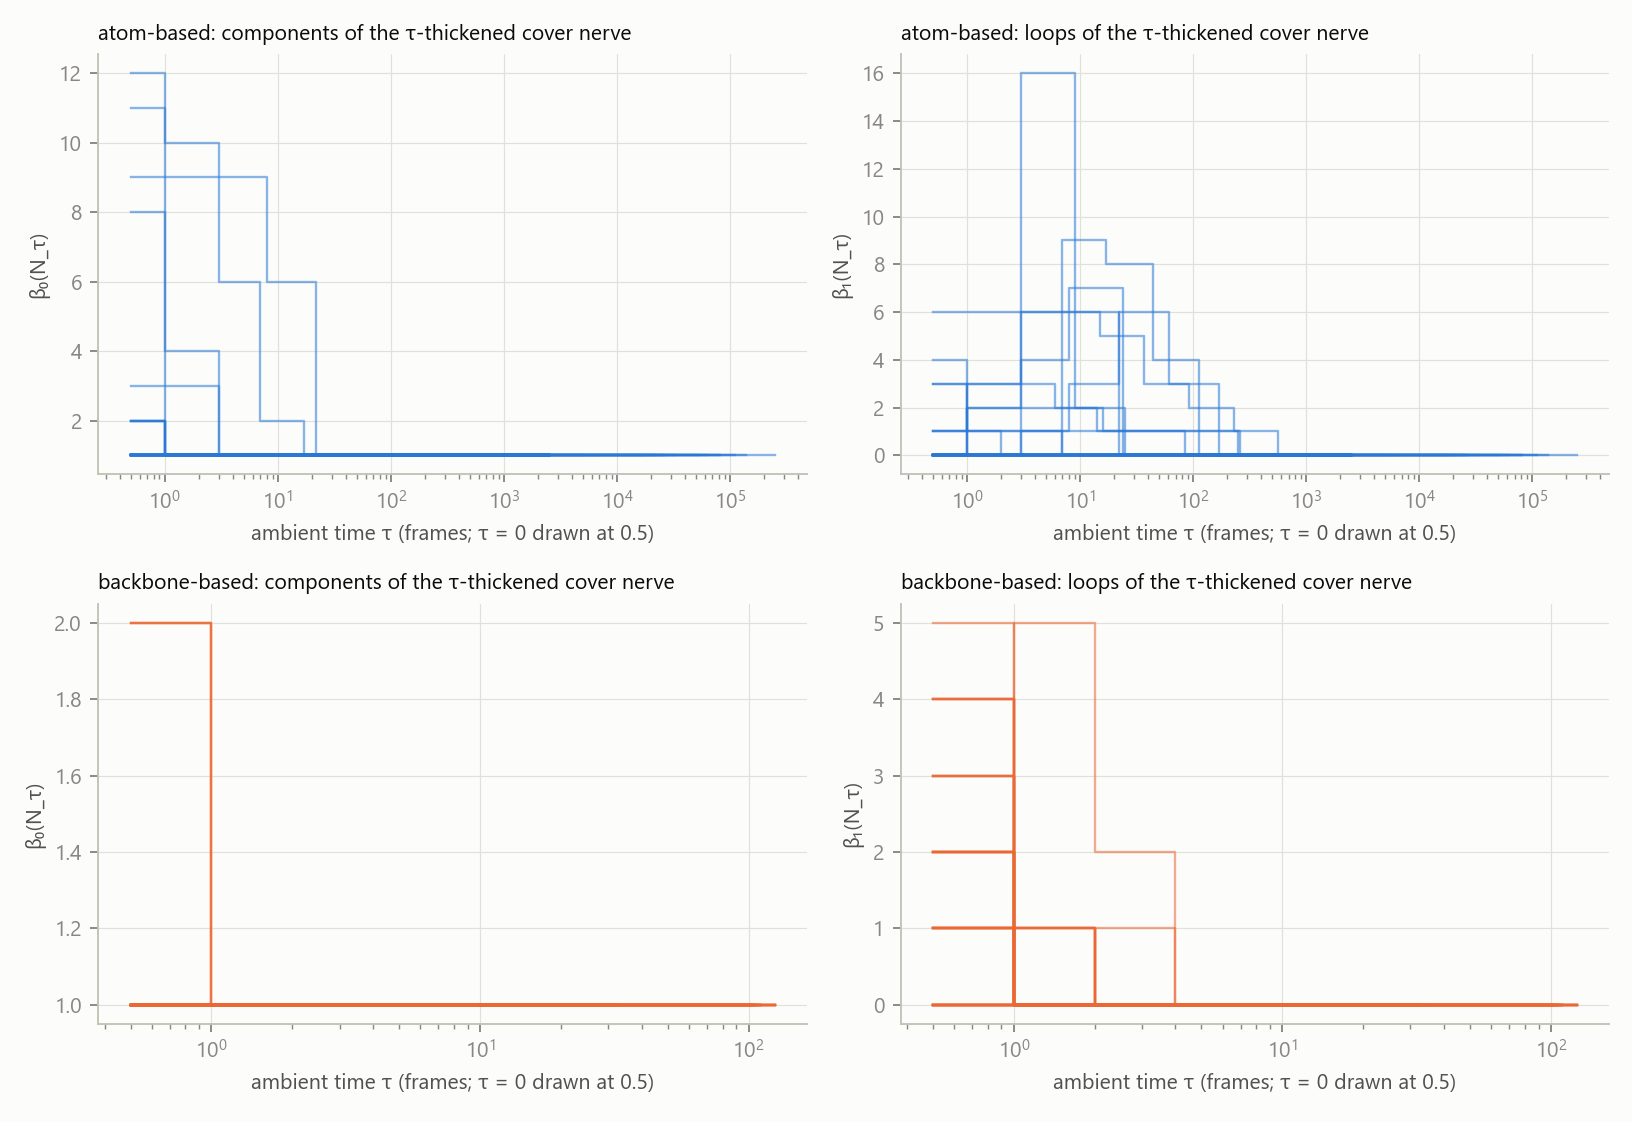
\includegraphics[width=.8\linewidth,height=.82\textheight,keepaspectratio]{comparison/fig_betti_curves.png}\caption{Fluid filtration: Betti numbers of the thickened cover nerve against ambient time.}\end{figure}\clearpage
\begin{figure}[H]\centering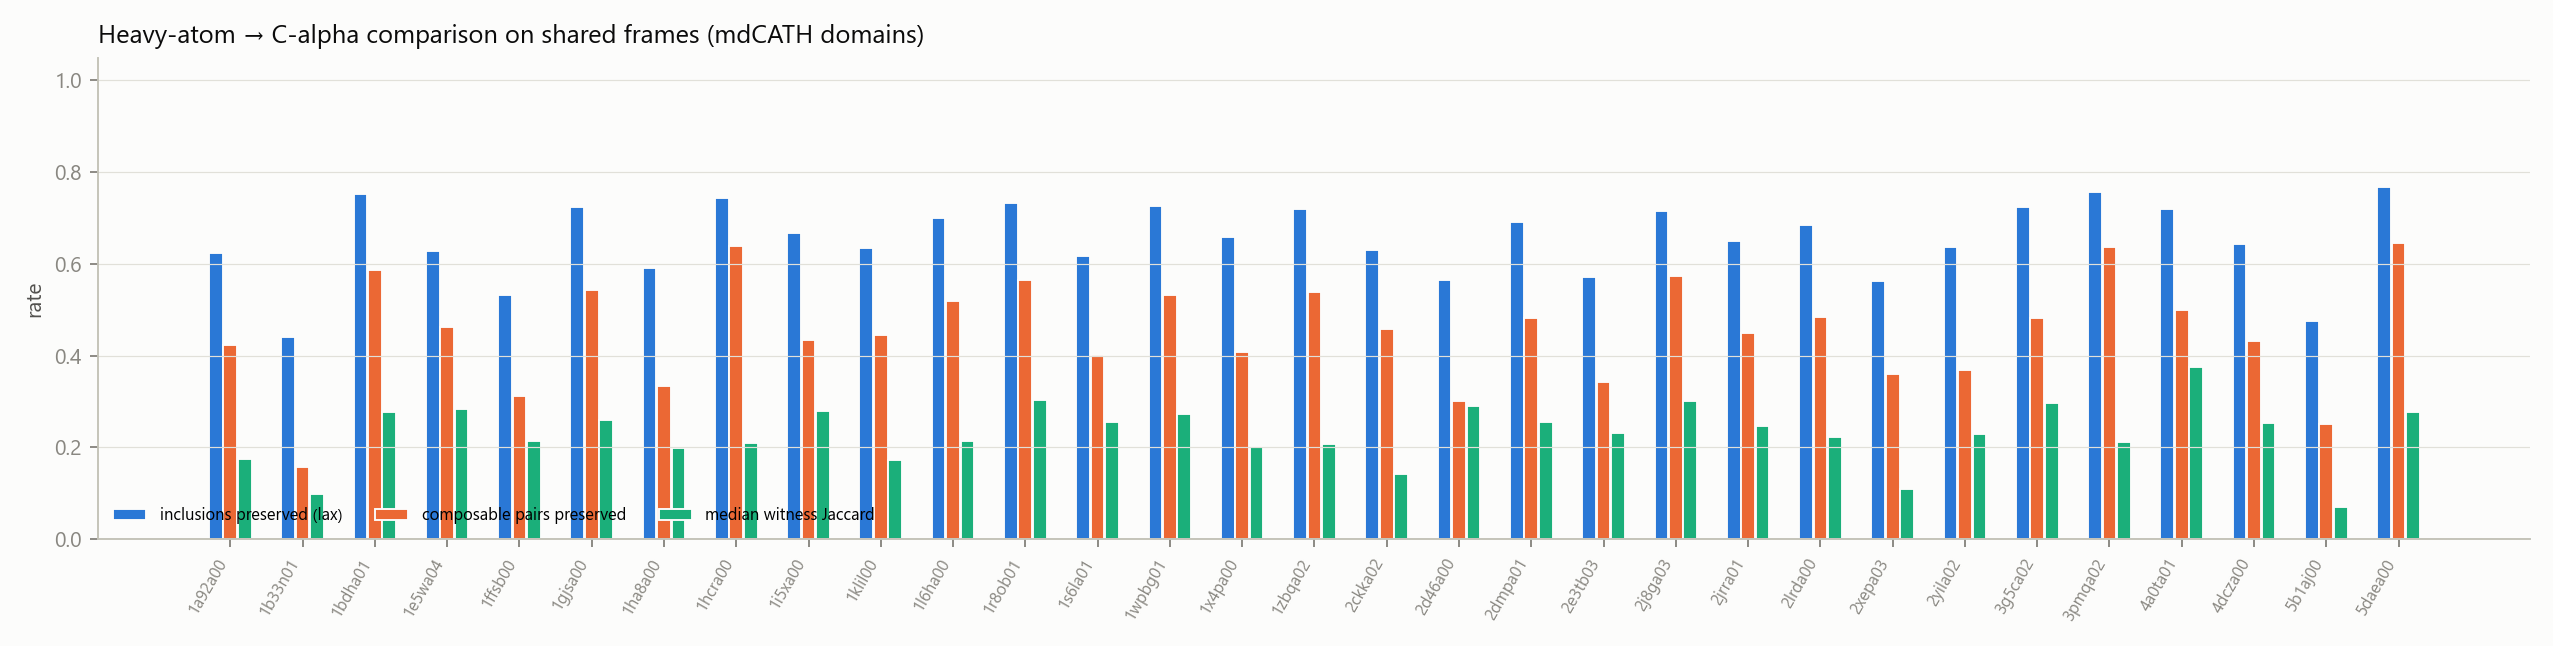
\includegraphics[width=.8\linewidth,height=.82\textheight,keepaspectratio]{comparison/fig_functor.png}\caption{Comparison of face posets from heavy atoms and from C$\alpha$ sites on identical frames (mdCATH).}\end{figure}\clearpage
\begin{figure}[H]\centering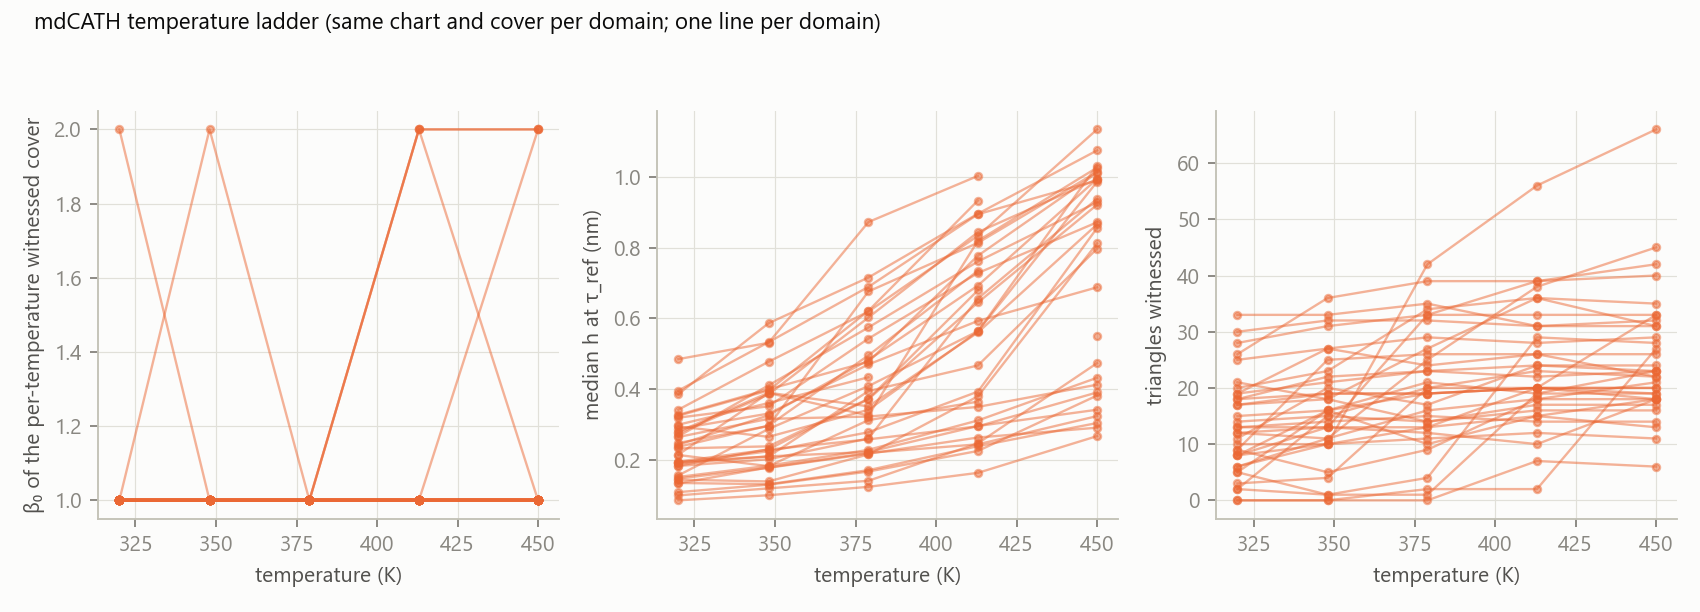
\includegraphics[width=.8\linewidth,height=.82\textheight,keepaspectratio]{comparison/fig_temperature.png}\caption{mdCATH temperature ladder.}\end{figure}\clearpage
\section*{Plates}
\begin{figure}[H]\centering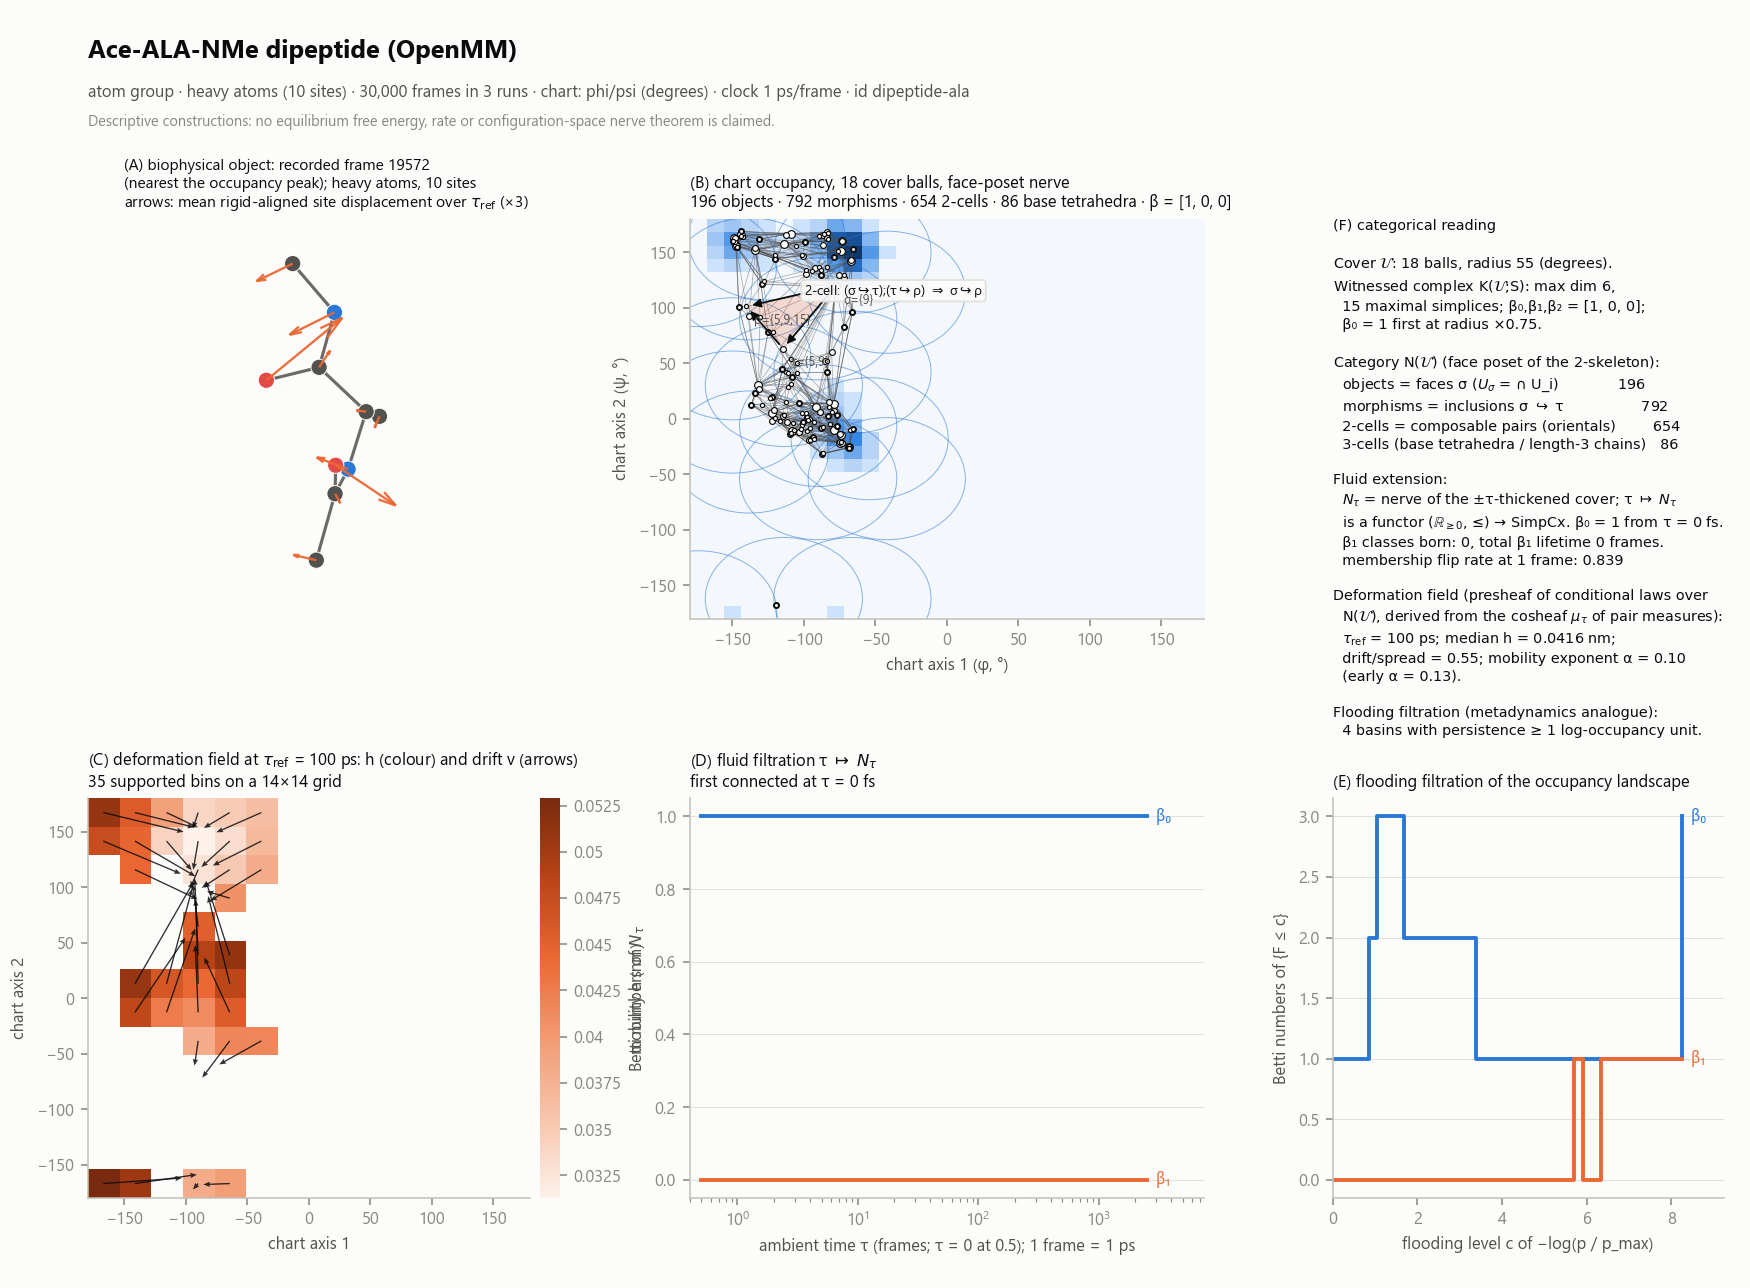
\includegraphics[width=\linewidth,height=.93\textheight,keepaspectratio]{systems/dipeptide-ala/plate.png}\caption{Ace-ALA-NMe dipeptide (OpenMM) (\texttt{dipeptide-ala}). Source: generate\_dipeptides.py (this repository).}\end{figure}\clearpage
\begin{figure}[H]\centering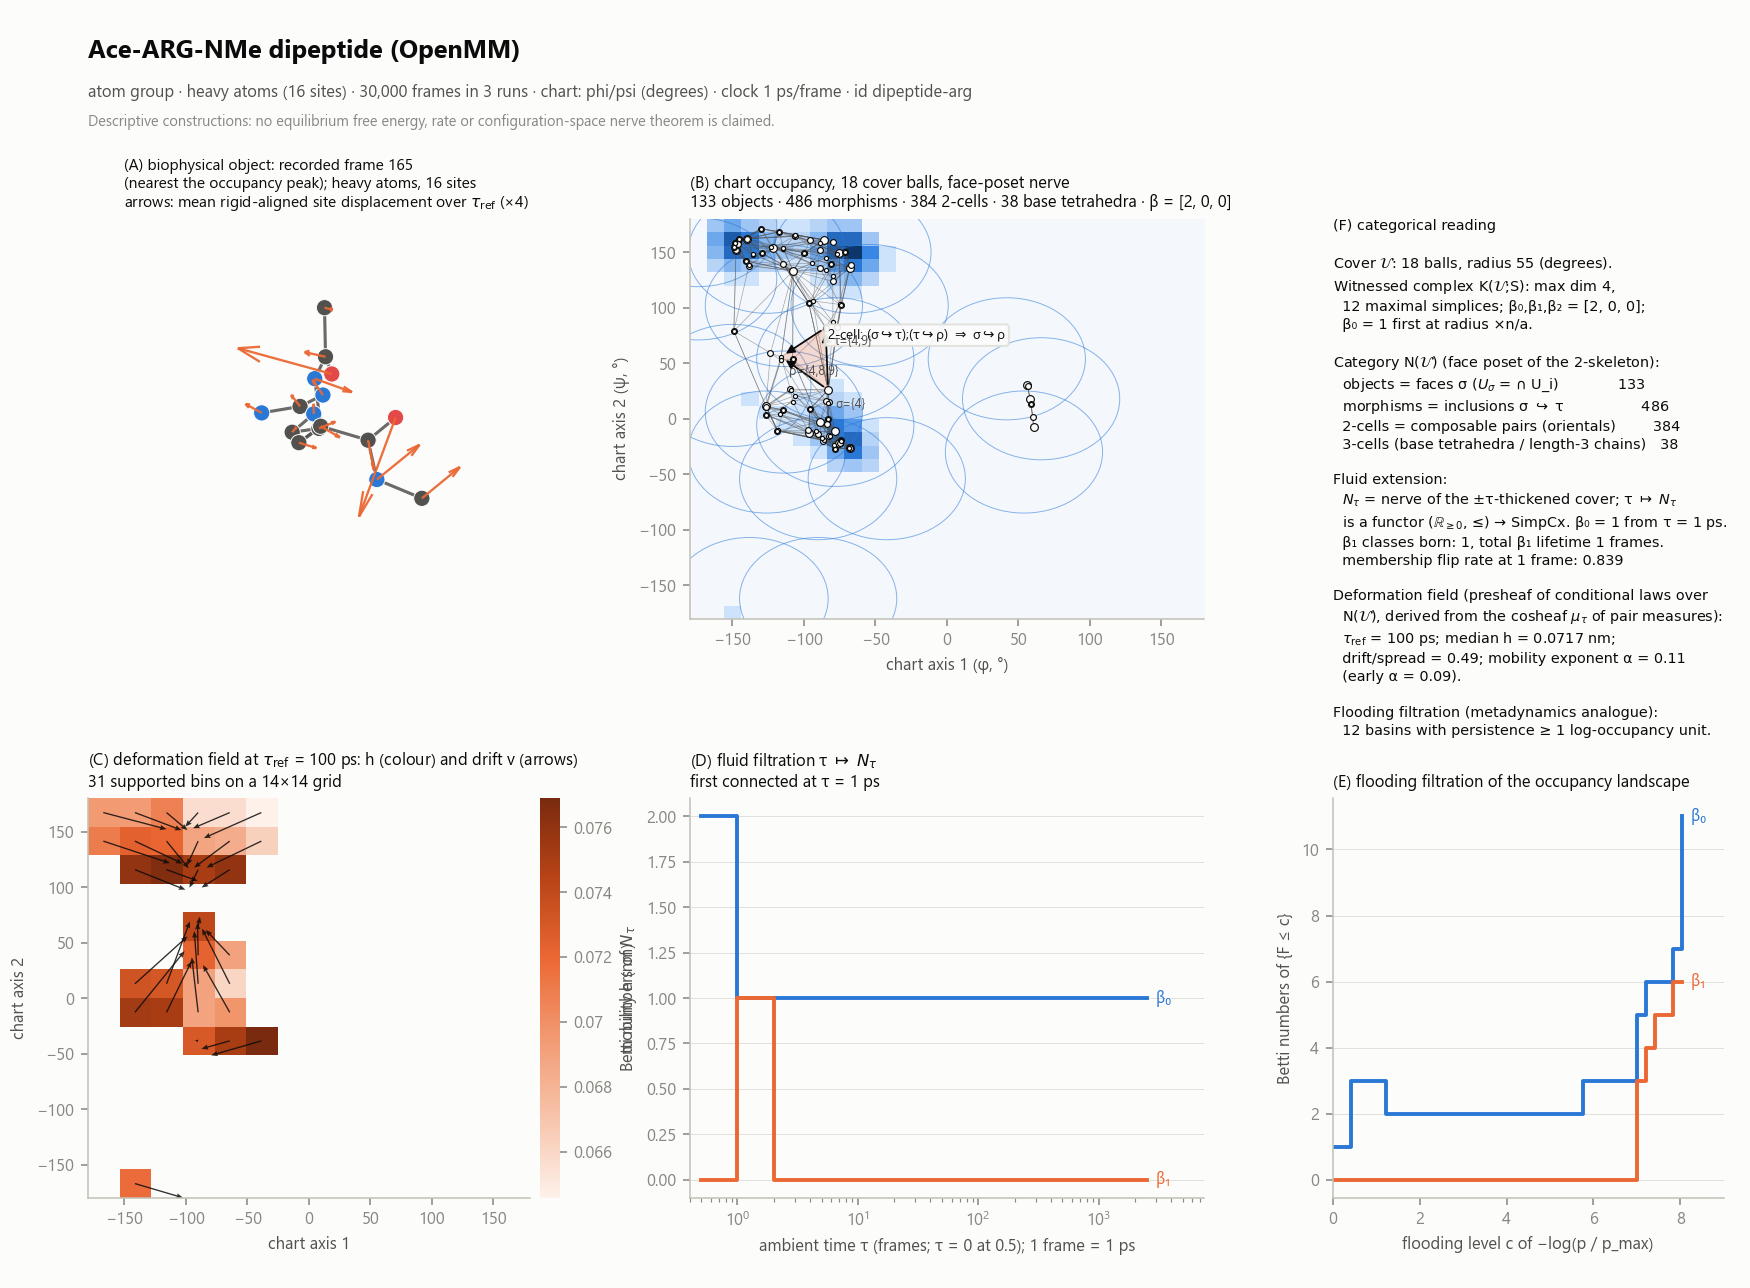
\includegraphics[width=\linewidth,height=.93\textheight,keepaspectratio]{systems/dipeptide-arg/plate.png}\caption{Ace-ARG-NMe dipeptide (OpenMM) (\texttt{dipeptide-arg}). Source: generate\_dipeptides.py (this repository).}\end{figure}\clearpage
\begin{figure}[H]\centering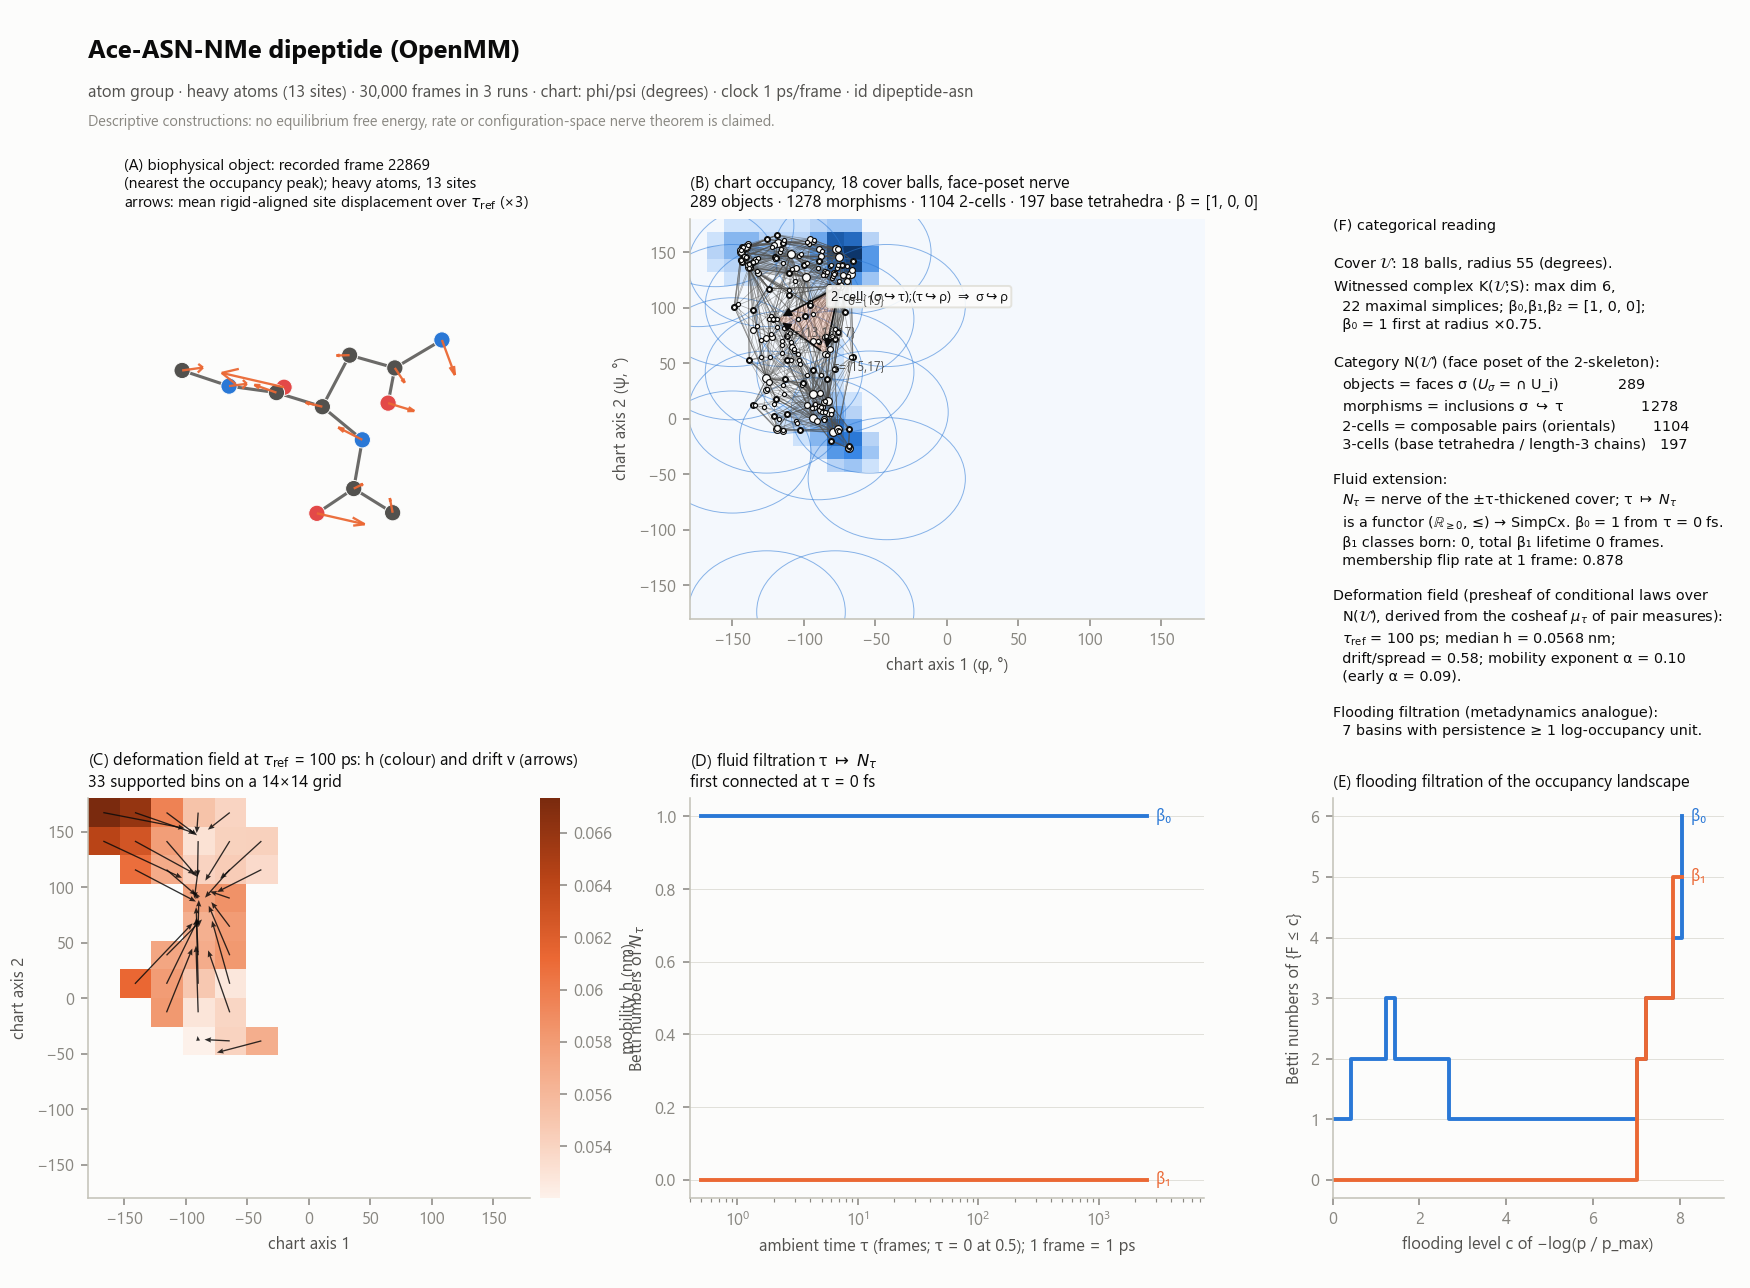
\includegraphics[width=\linewidth,height=.93\textheight,keepaspectratio]{systems/dipeptide-asn/plate.png}\caption{Ace-ASN-NMe dipeptide (OpenMM) (\texttt{dipeptide-asn}). Source: generate\_dipeptides.py (this repository).}\end{figure}\clearpage
\begin{figure}[H]\centering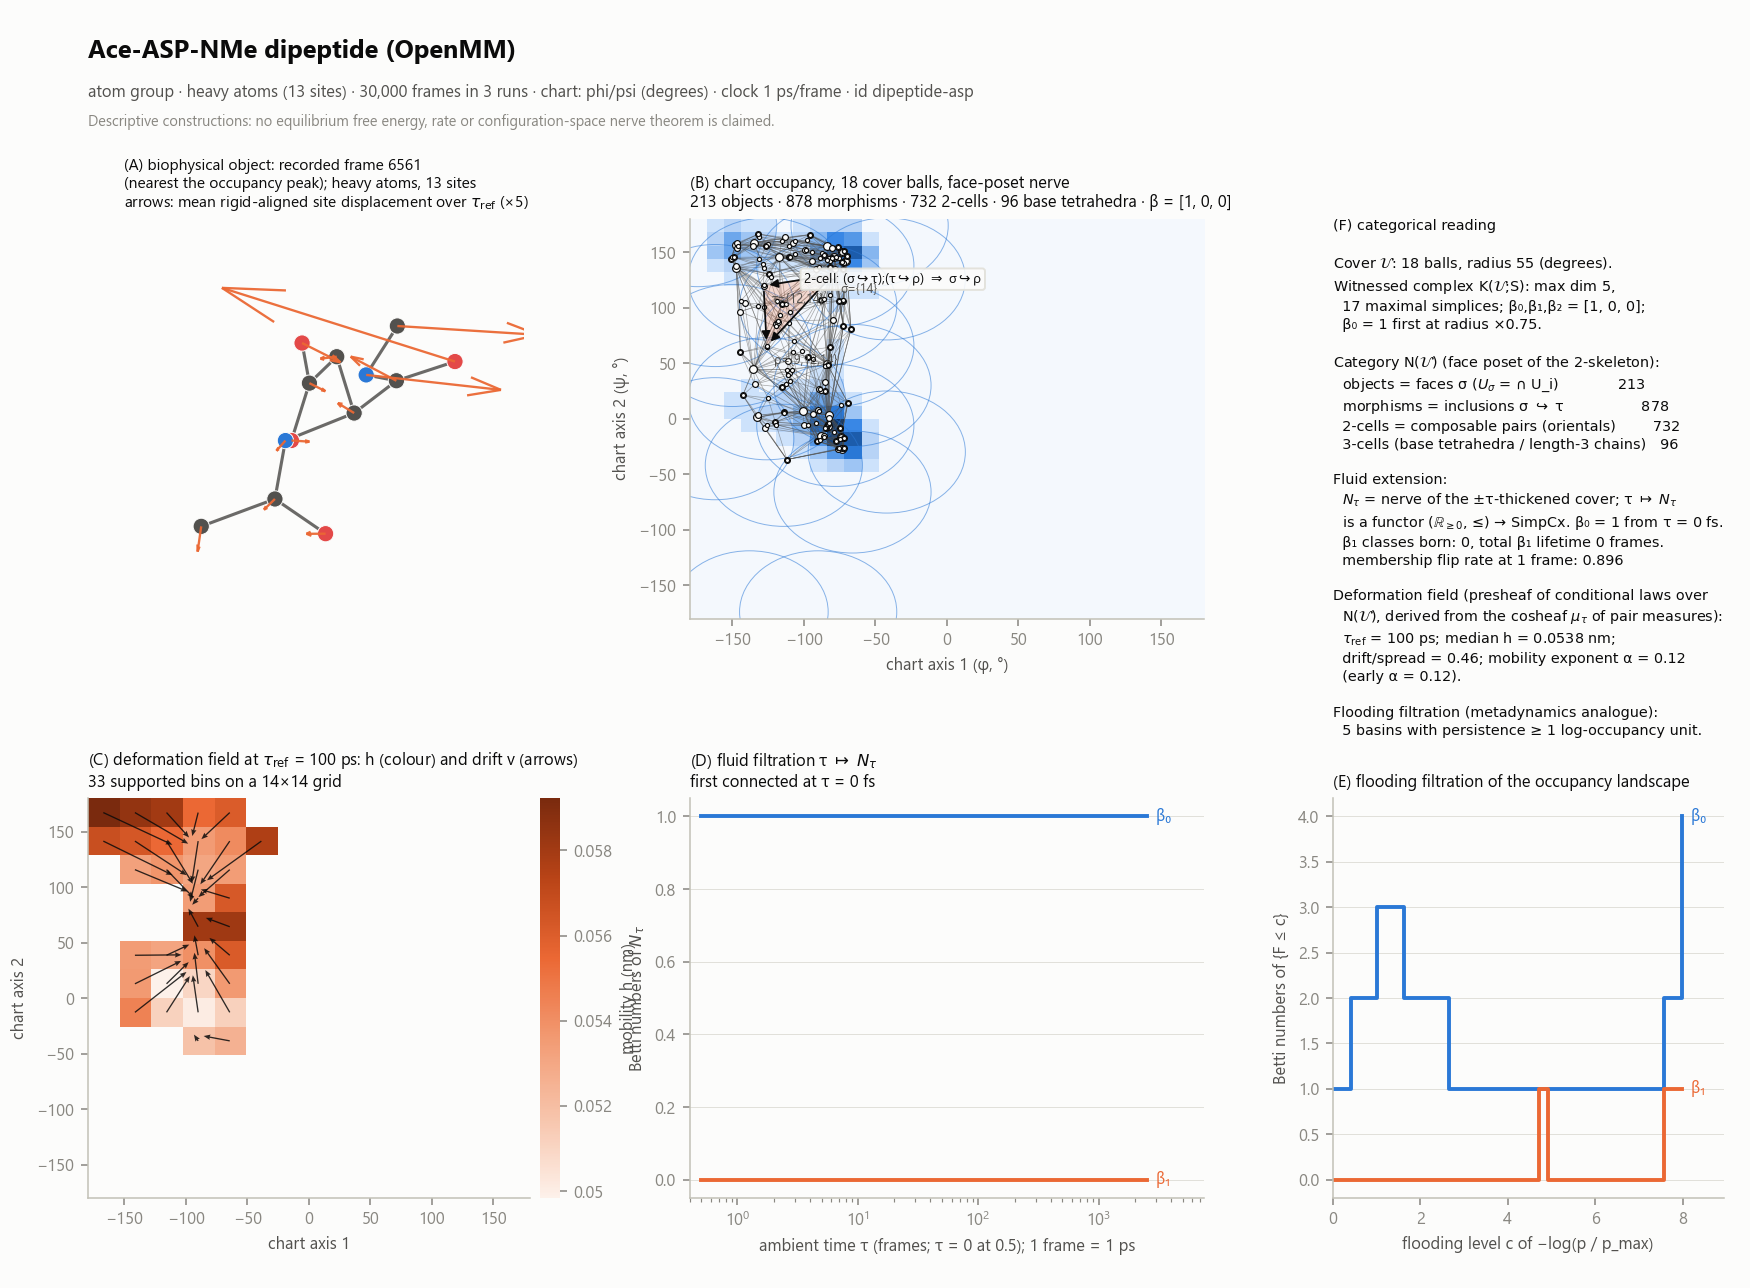
\includegraphics[width=\linewidth,height=.93\textheight,keepaspectratio]{systems/dipeptide-asp/plate.png}\caption{Ace-ASP-NMe dipeptide (OpenMM) (\texttt{dipeptide-asp}). Source: generate\_dipeptides.py (this repository).}\end{figure}\clearpage
\begin{figure}[H]\centering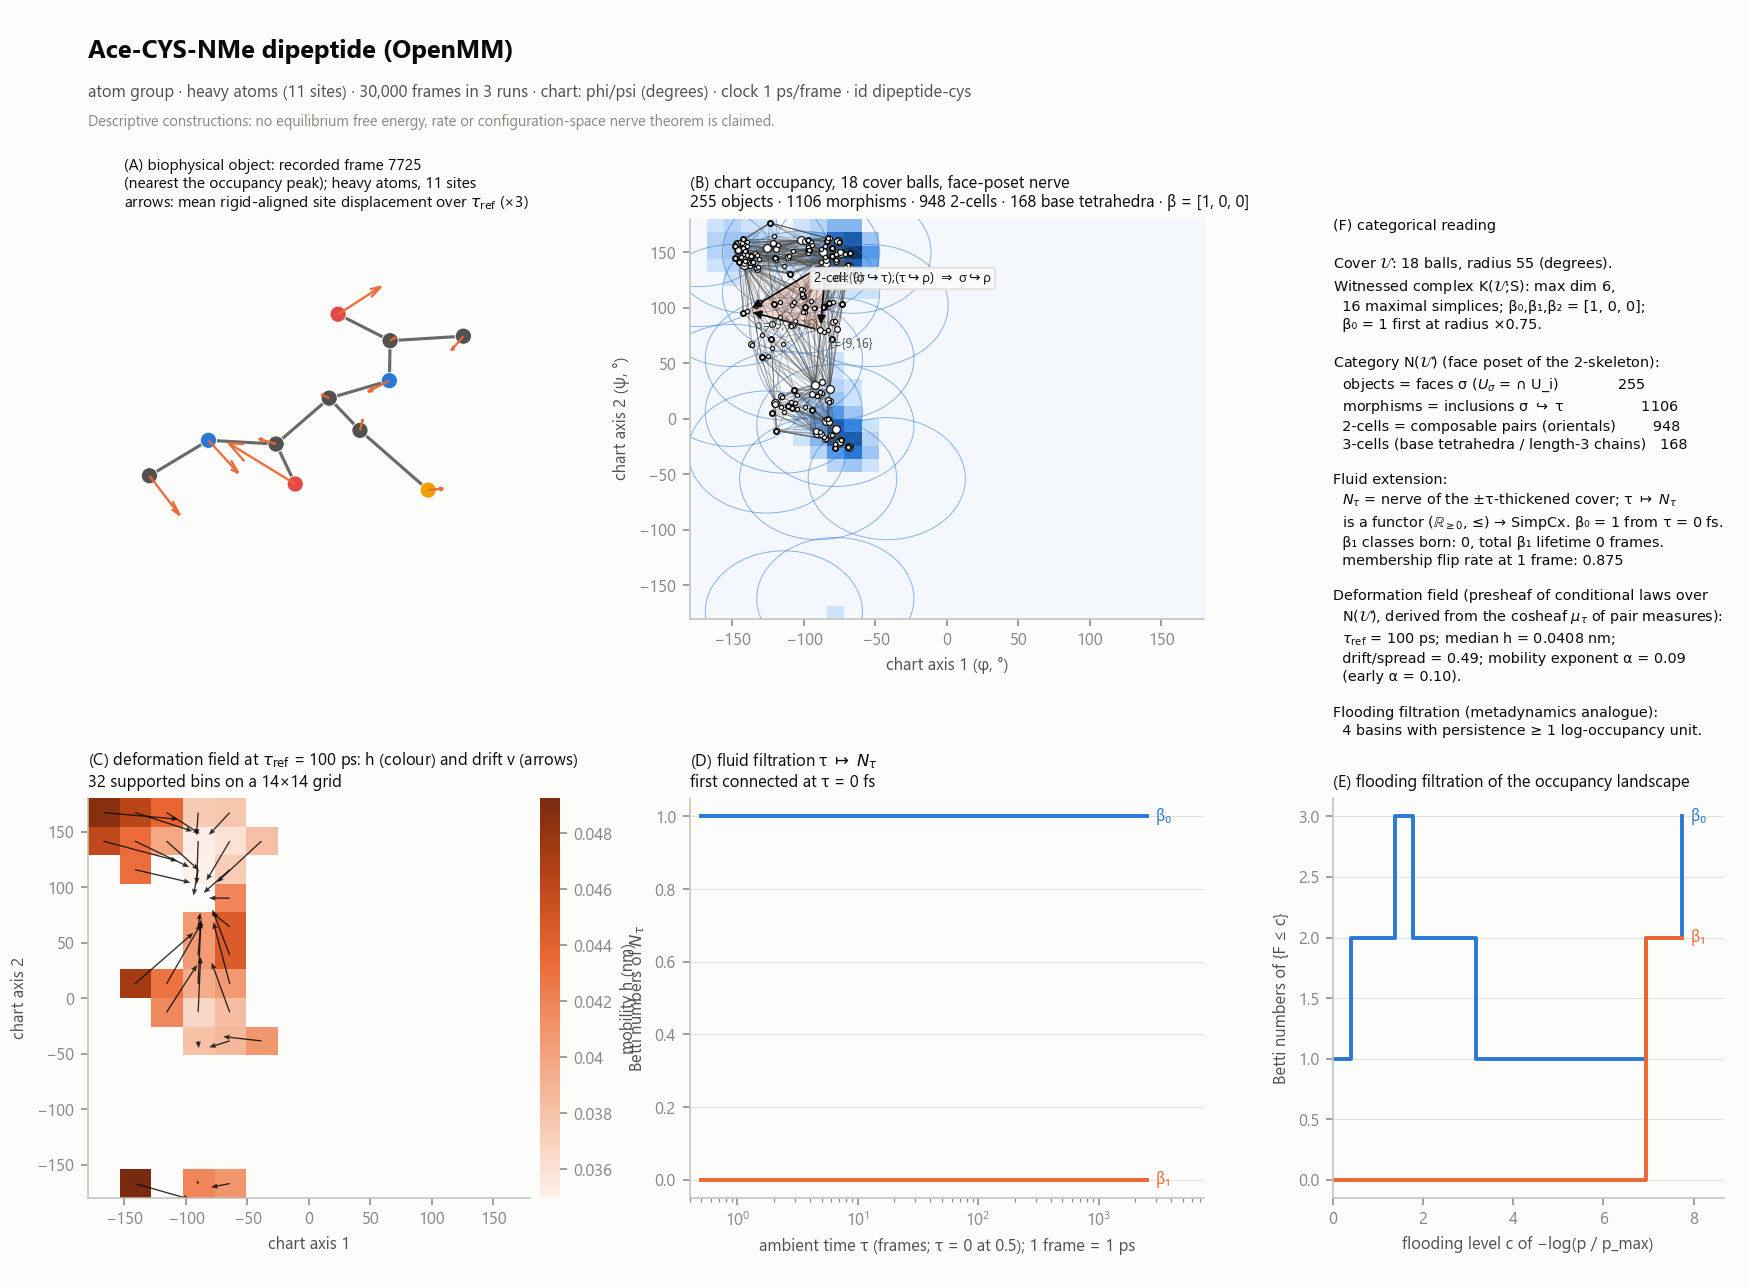
\includegraphics[width=\linewidth,height=.93\textheight,keepaspectratio]{systems/dipeptide-cys/plate.png}\caption{Ace-CYS-NMe dipeptide (OpenMM) (\texttt{dipeptide-cys}). Source: generate\_dipeptides.py (this repository).}\end{figure}\clearpage
\begin{figure}[H]\centering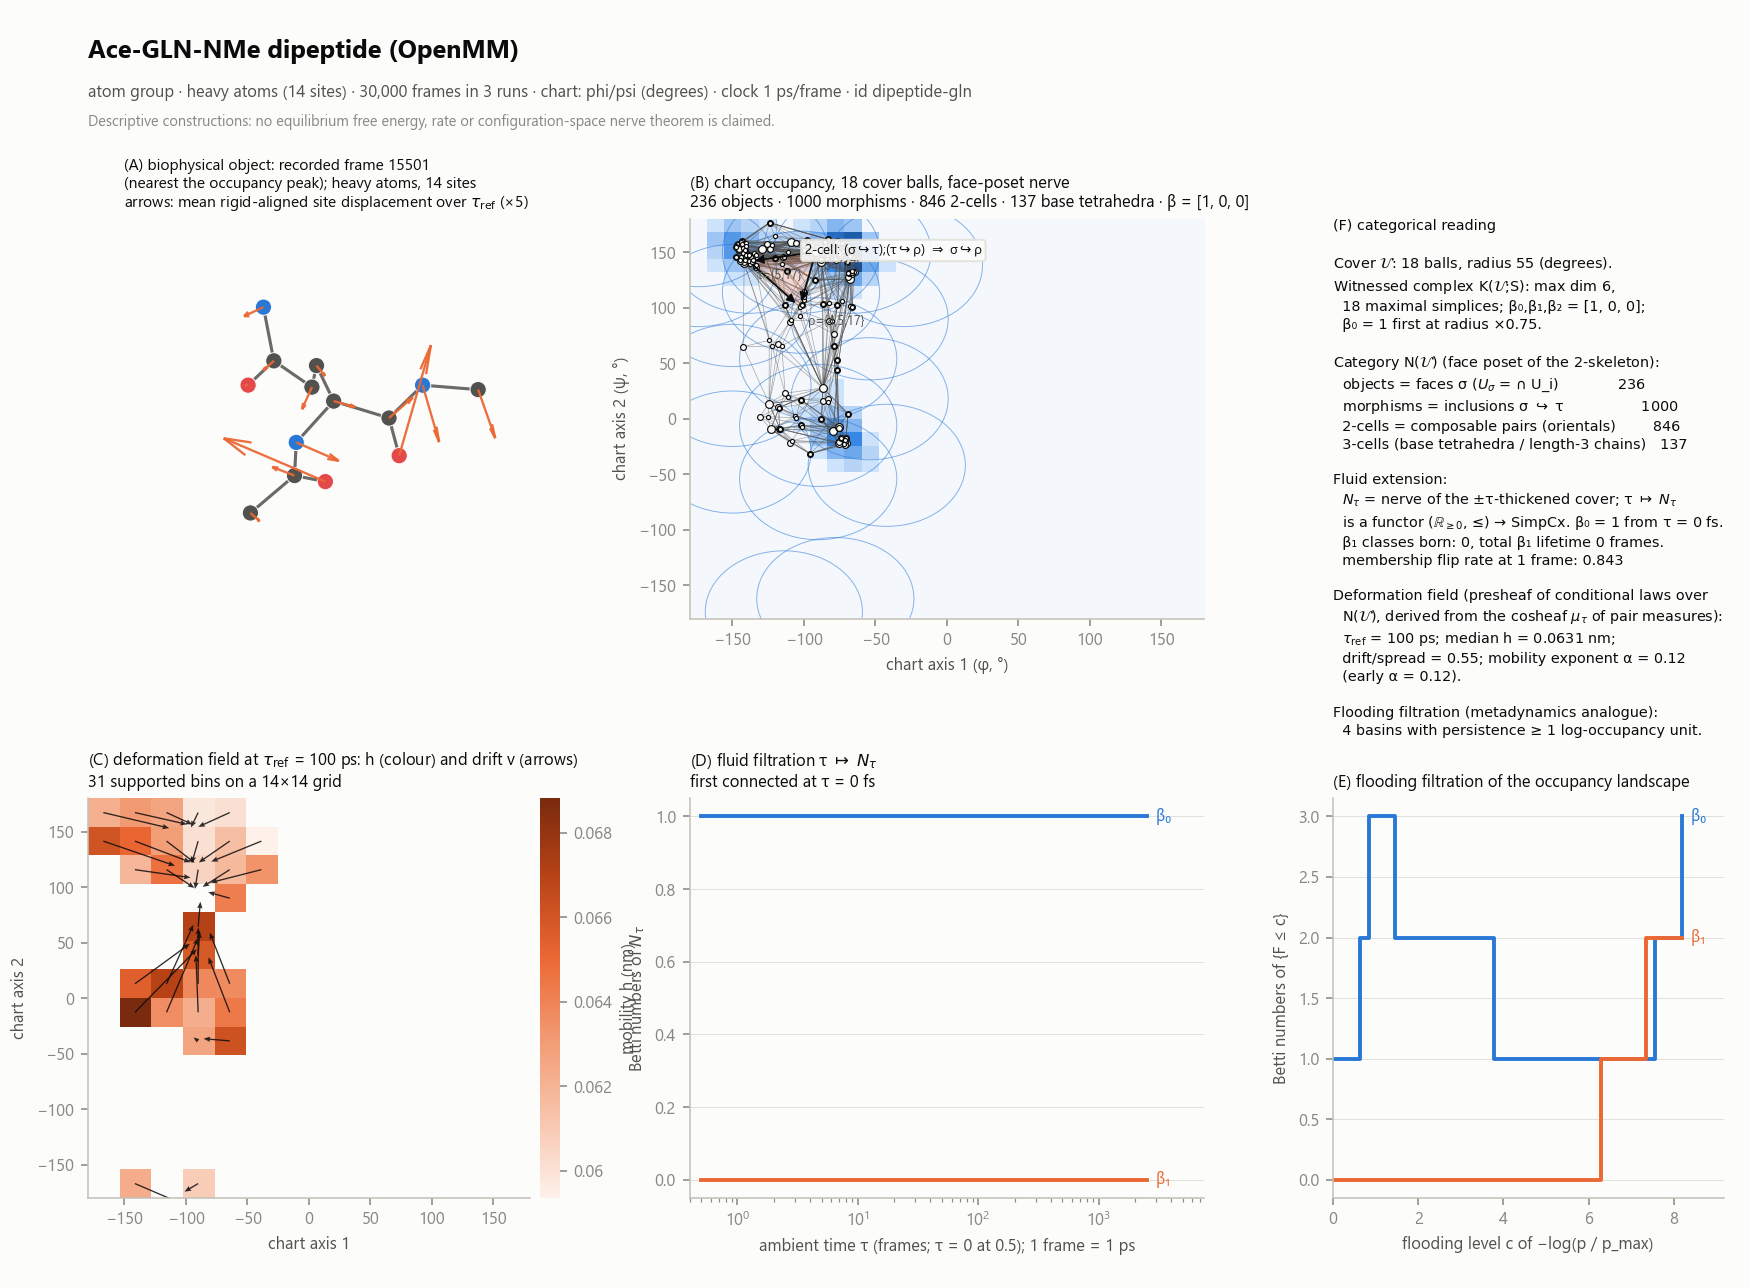
\includegraphics[width=\linewidth,height=.93\textheight,keepaspectratio]{systems/dipeptide-gln/plate.png}\caption{Ace-GLN-NMe dipeptide (OpenMM) (\texttt{dipeptide-gln}). Source: generate\_dipeptides.py (this repository).}\end{figure}\clearpage
\begin{figure}[H]\centering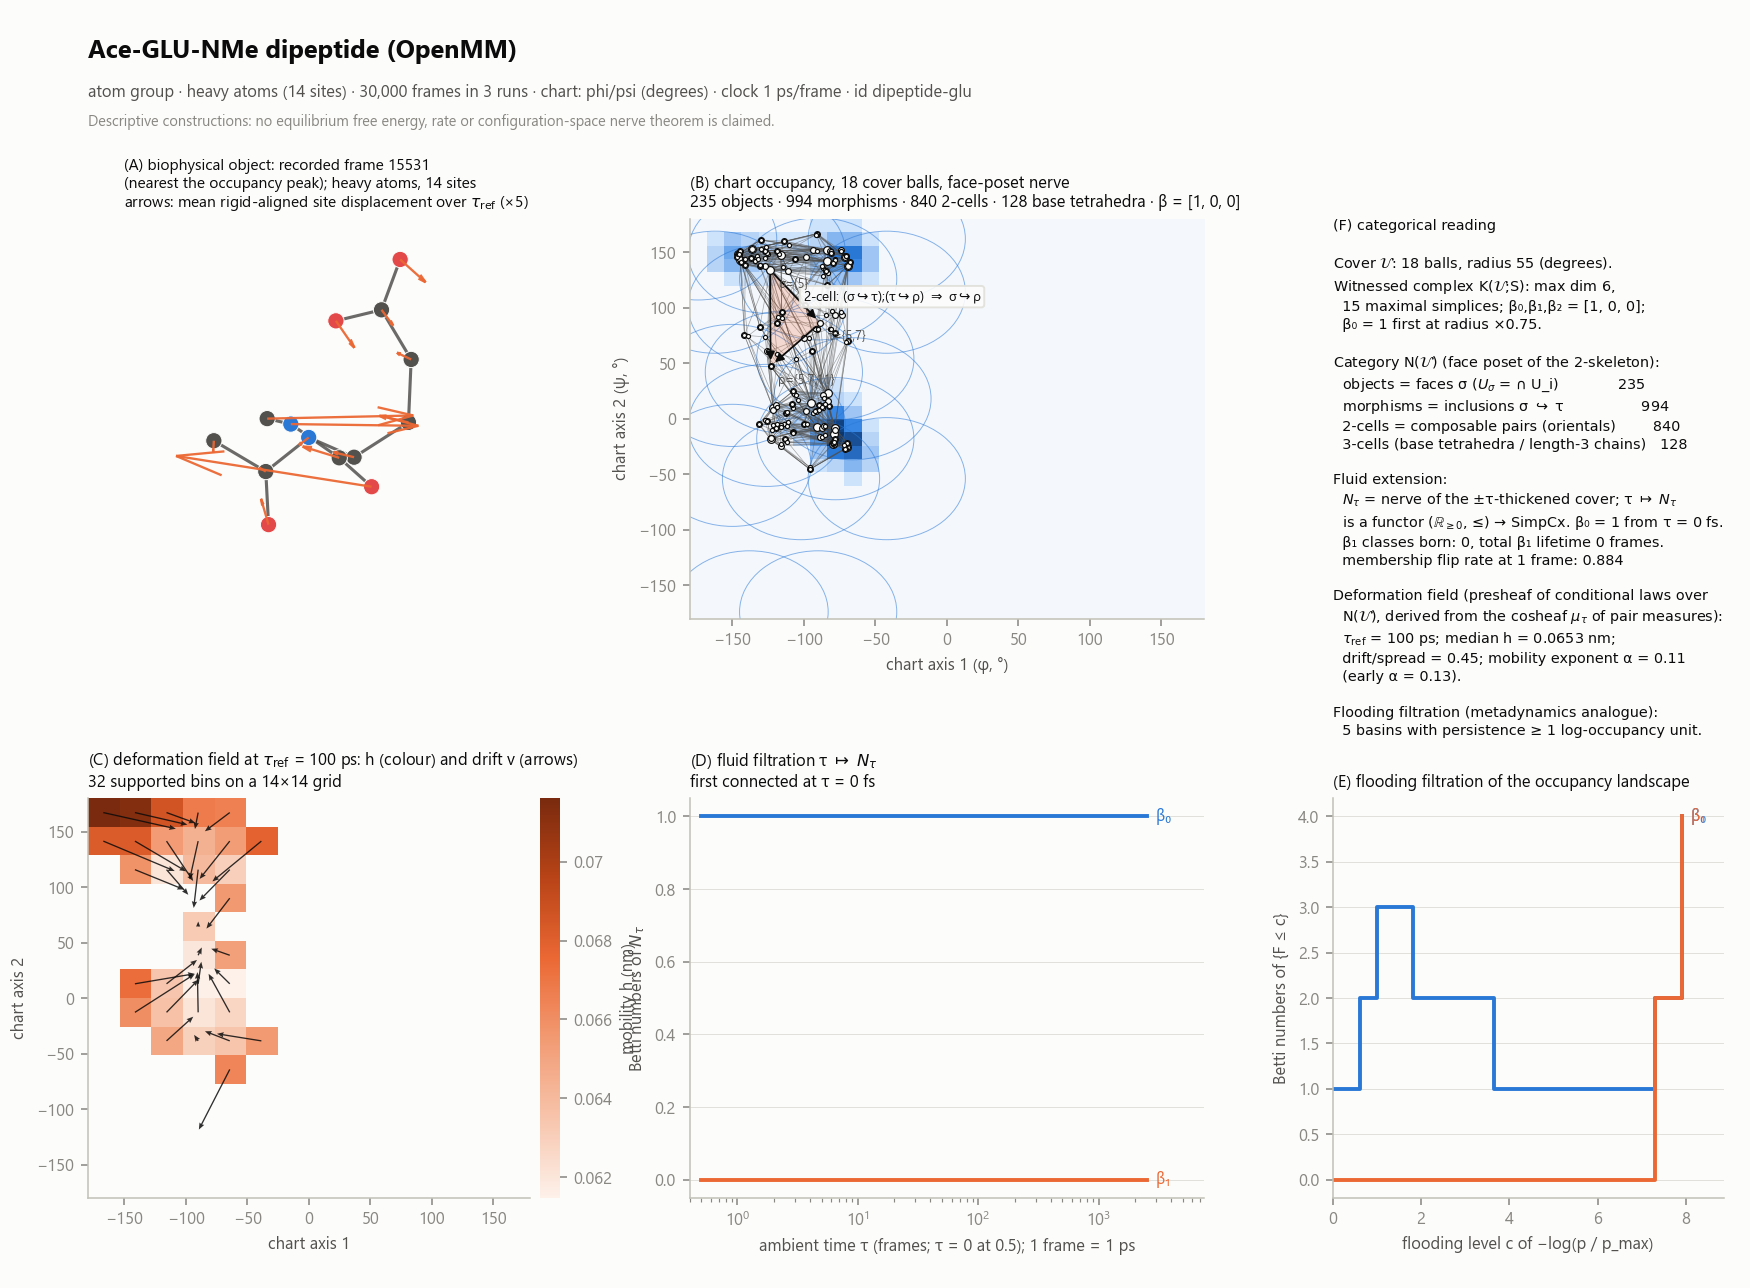
\includegraphics[width=\linewidth,height=.93\textheight,keepaspectratio]{systems/dipeptide-glu/plate.png}\caption{Ace-GLU-NMe dipeptide (OpenMM) (\texttt{dipeptide-glu}). Source: generate\_dipeptides.py (this repository).}\end{figure}\clearpage
\begin{figure}[H]\centering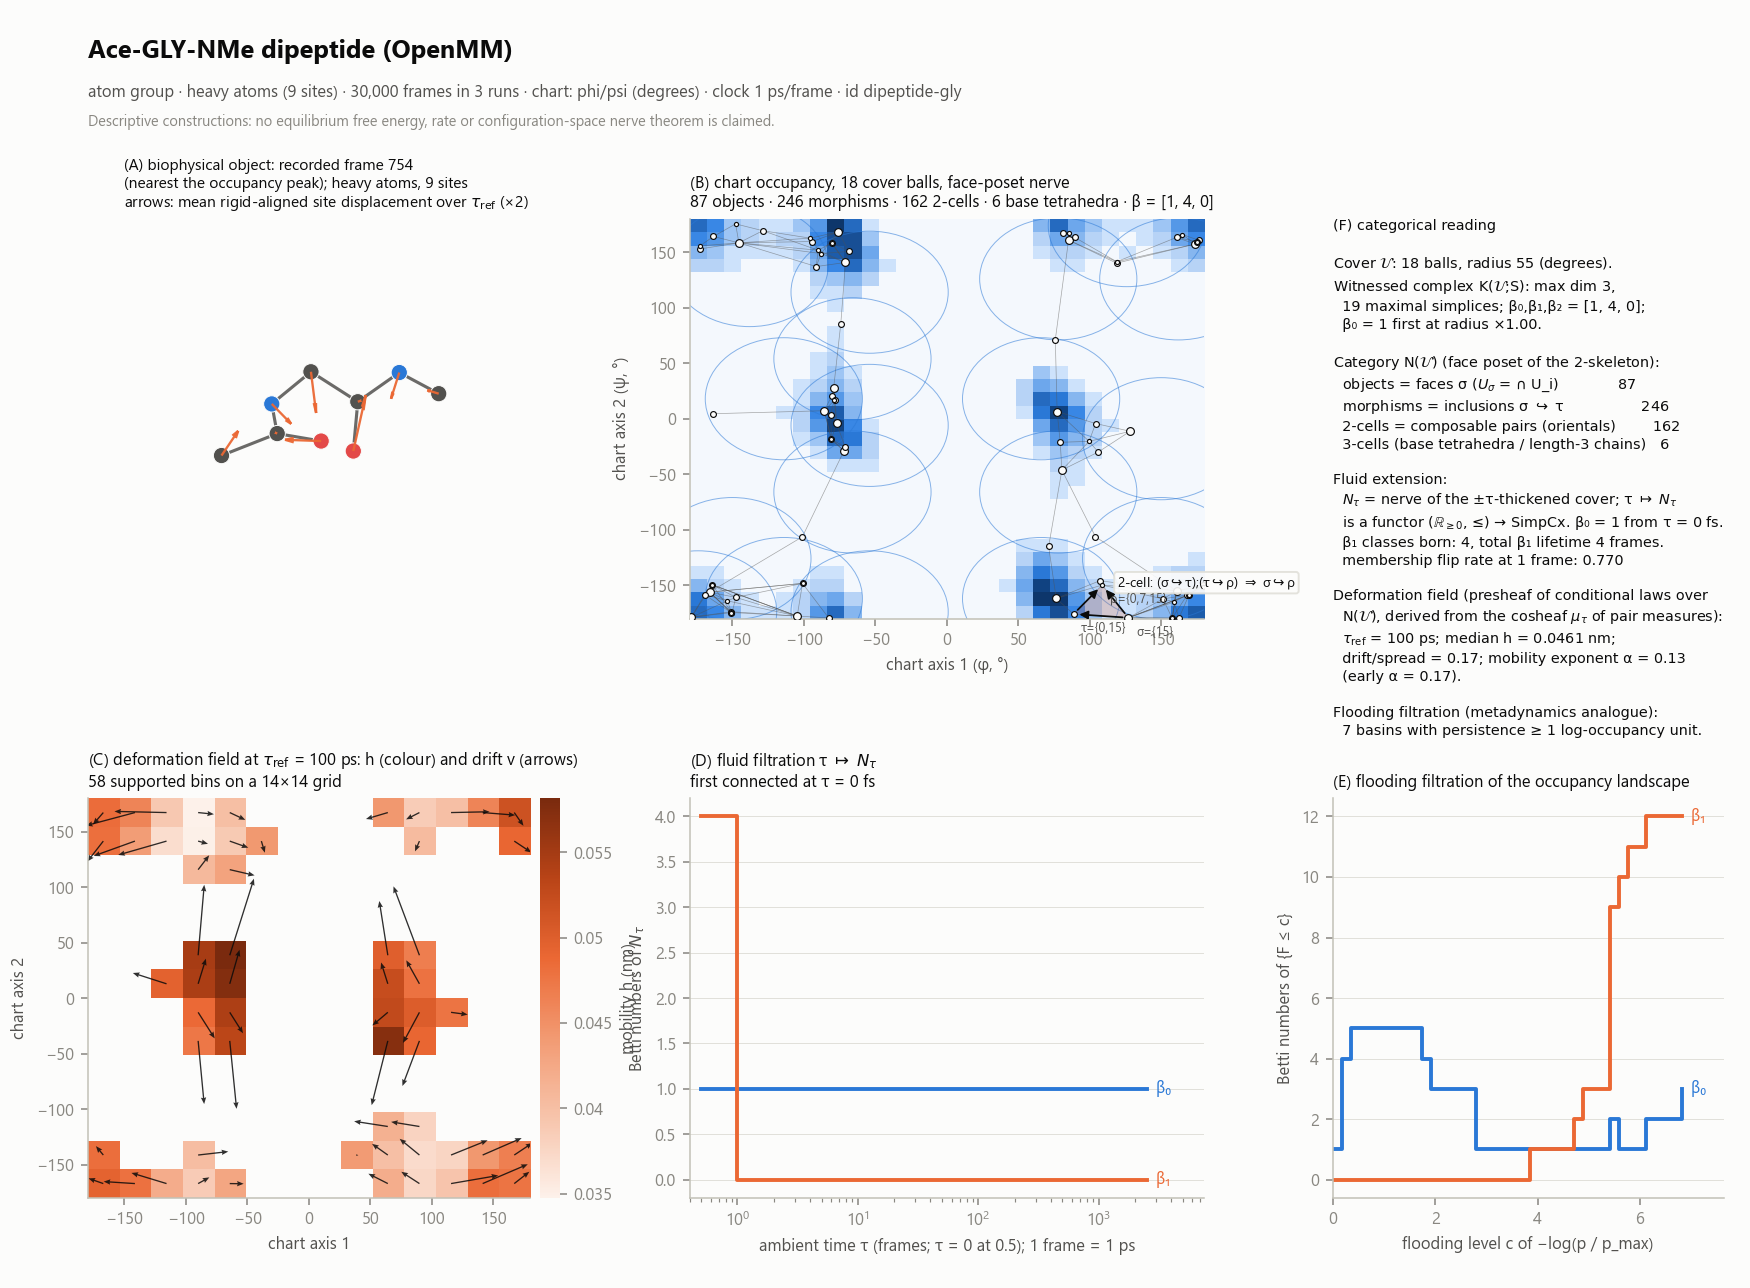
\includegraphics[width=\linewidth,height=.93\textheight,keepaspectratio]{systems/dipeptide-gly/plate.png}\caption{Ace-GLY-NMe dipeptide (OpenMM) (\texttt{dipeptide-gly}). Source: generate\_dipeptides.py (this repository).}\end{figure}\clearpage
\begin{figure}[H]\centering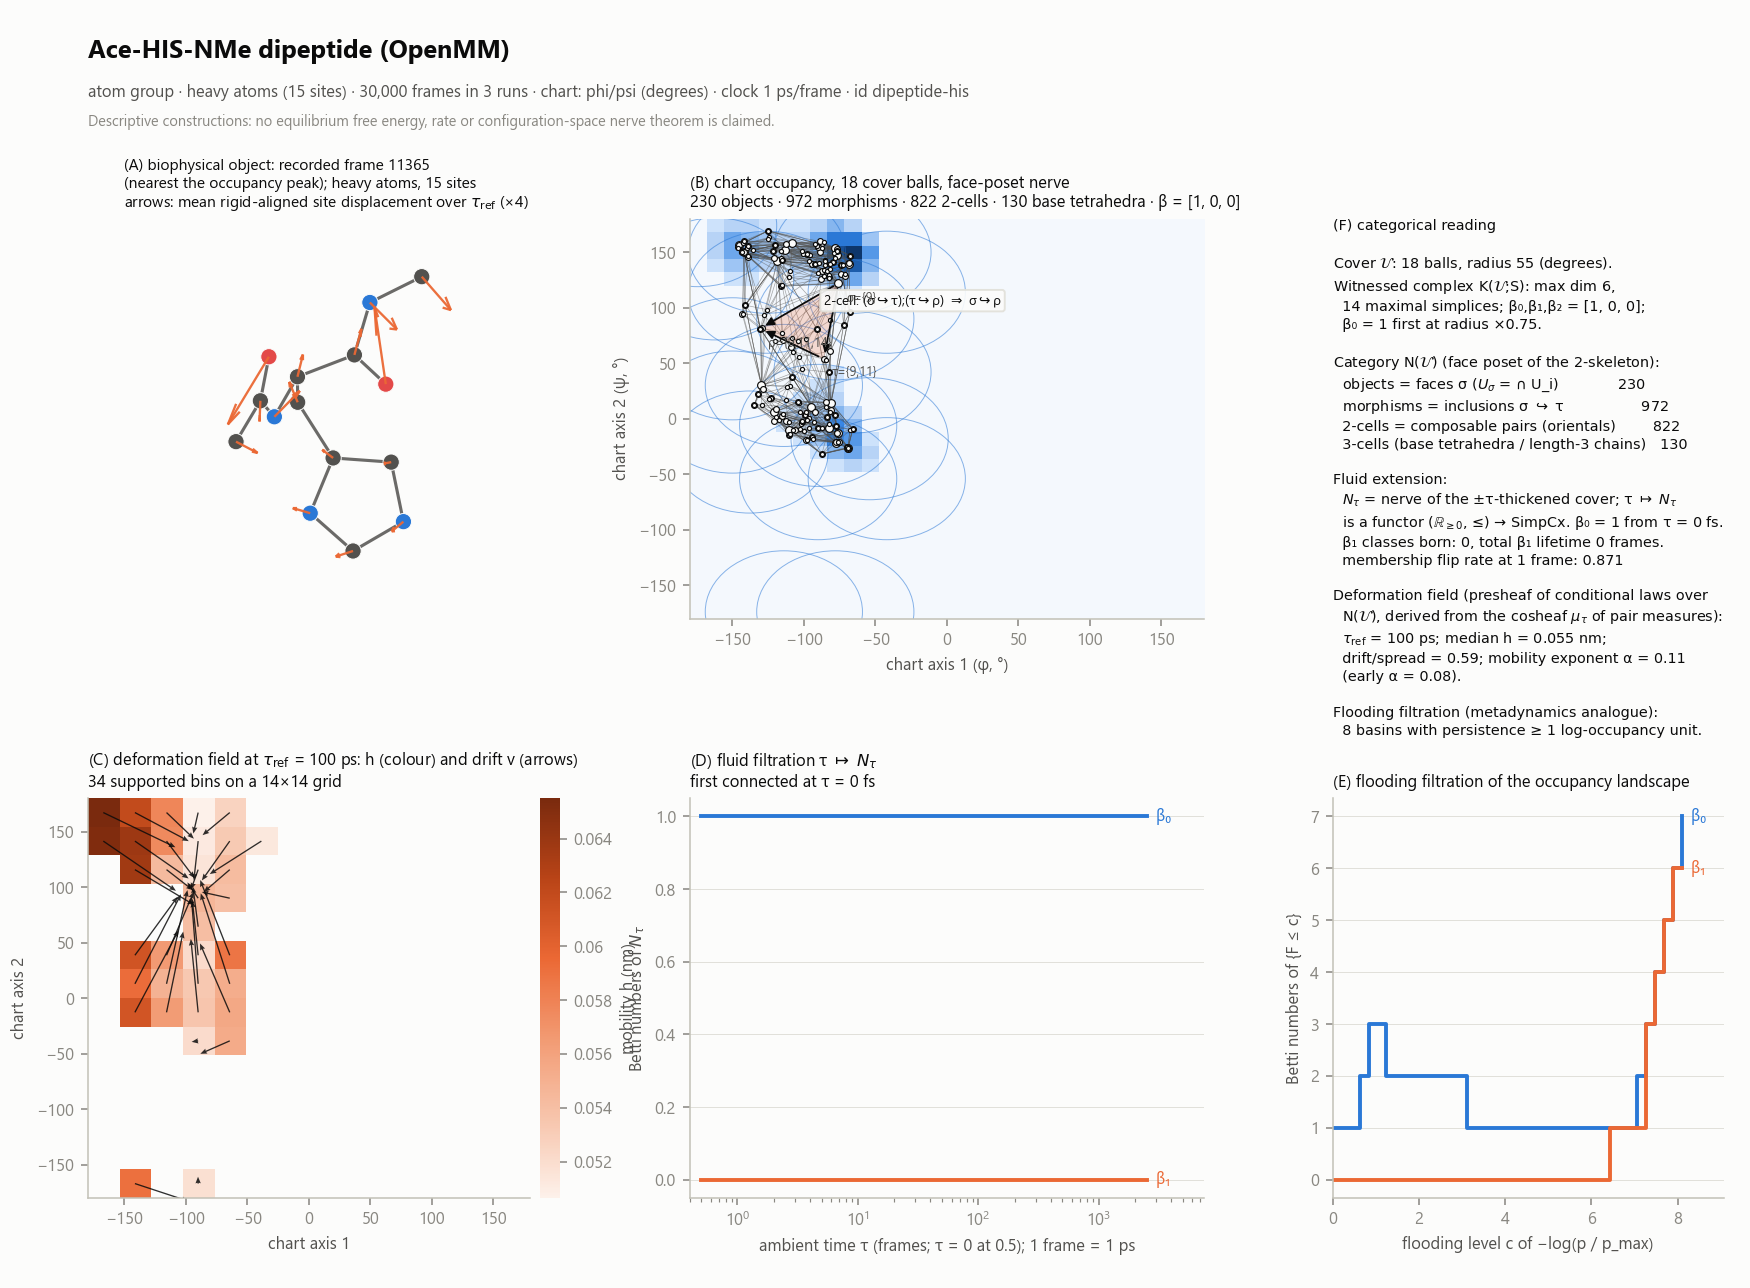
\includegraphics[width=\linewidth,height=.93\textheight,keepaspectratio]{systems/dipeptide-his/plate.png}\caption{Ace-HIS-NMe dipeptide (OpenMM) (\texttt{dipeptide-his}). Source: generate\_dipeptides.py (this repository).}\end{figure}\clearpage
\begin{figure}[H]\centering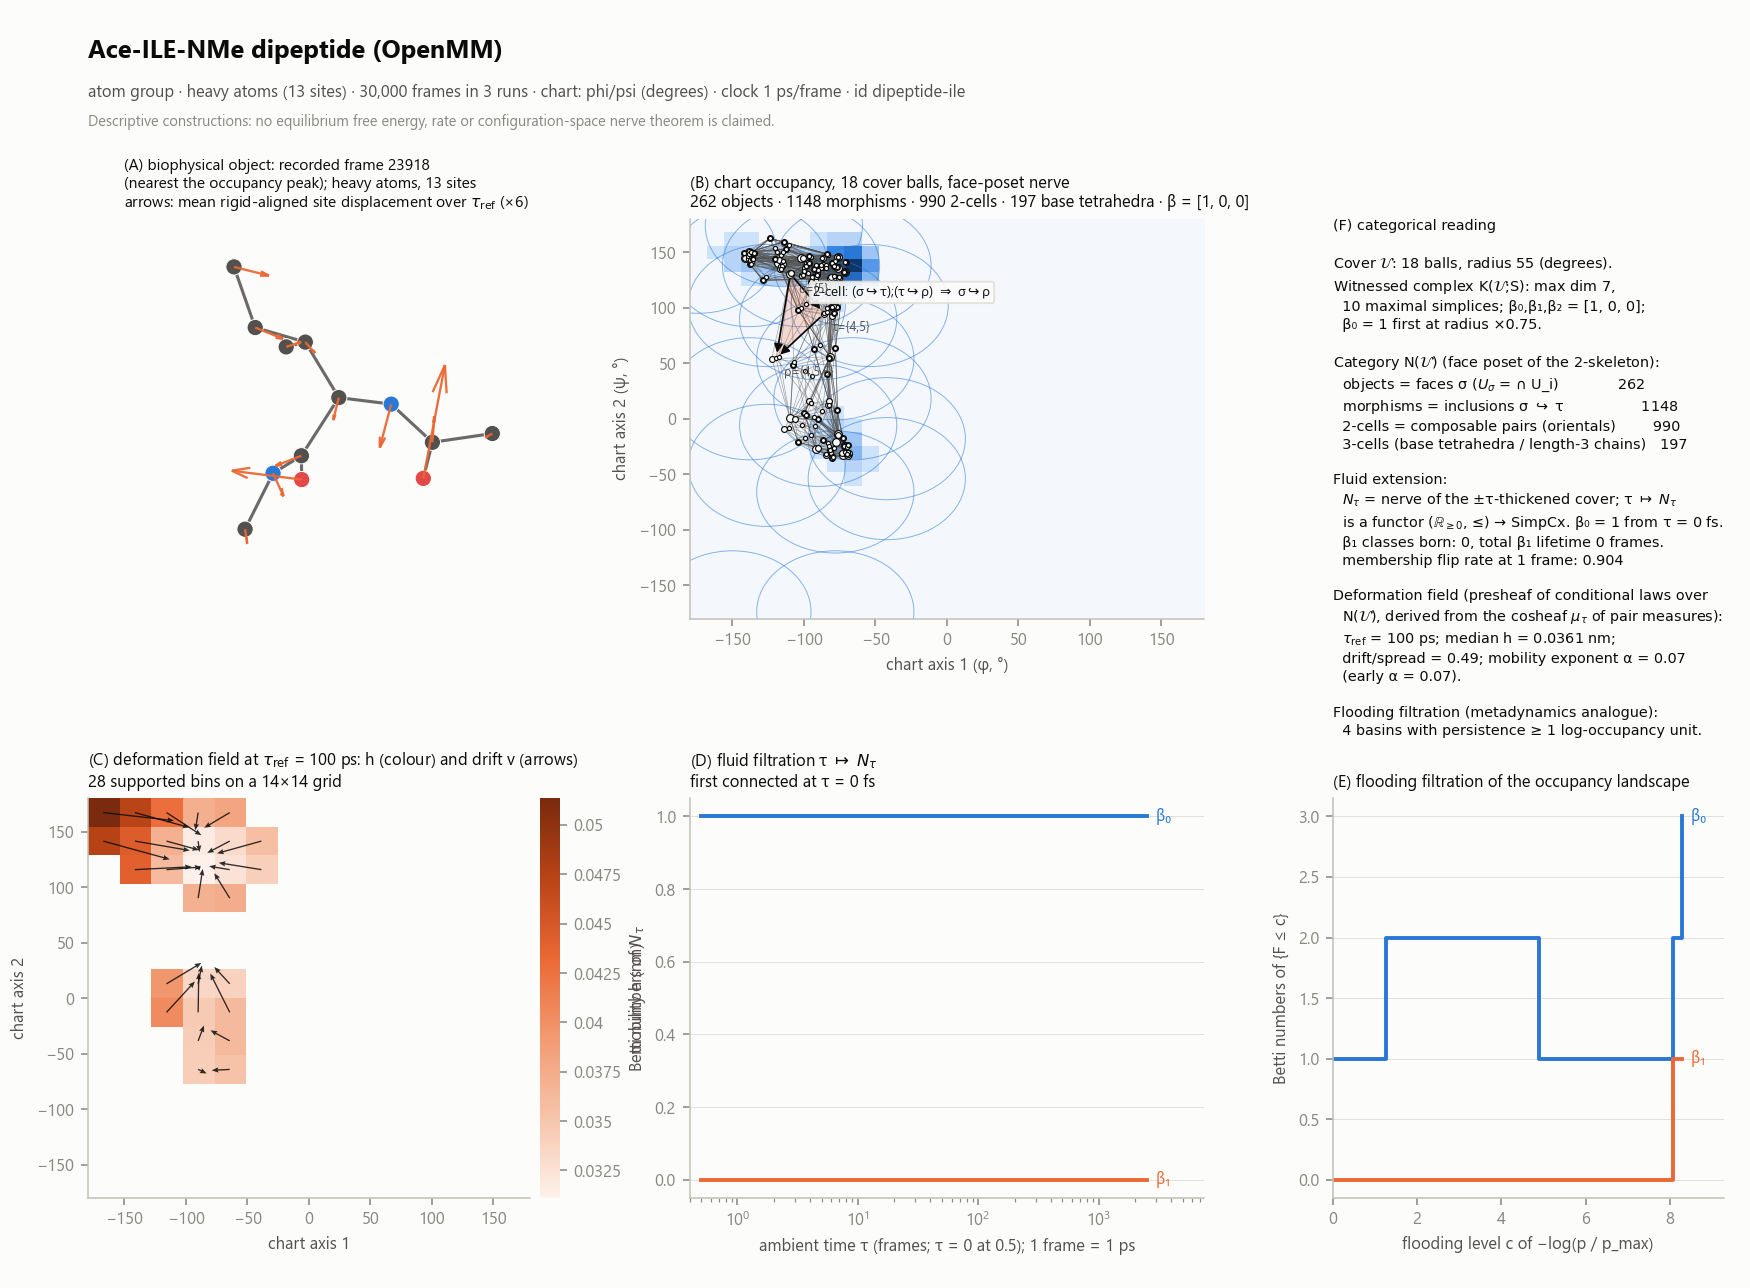
\includegraphics[width=\linewidth,height=.93\textheight,keepaspectratio]{systems/dipeptide-ile/plate.png}\caption{Ace-ILE-NMe dipeptide (OpenMM) (\texttt{dipeptide-ile}). Source: generate\_dipeptides.py (this repository).}\end{figure}\clearpage
\begin{figure}[H]\centering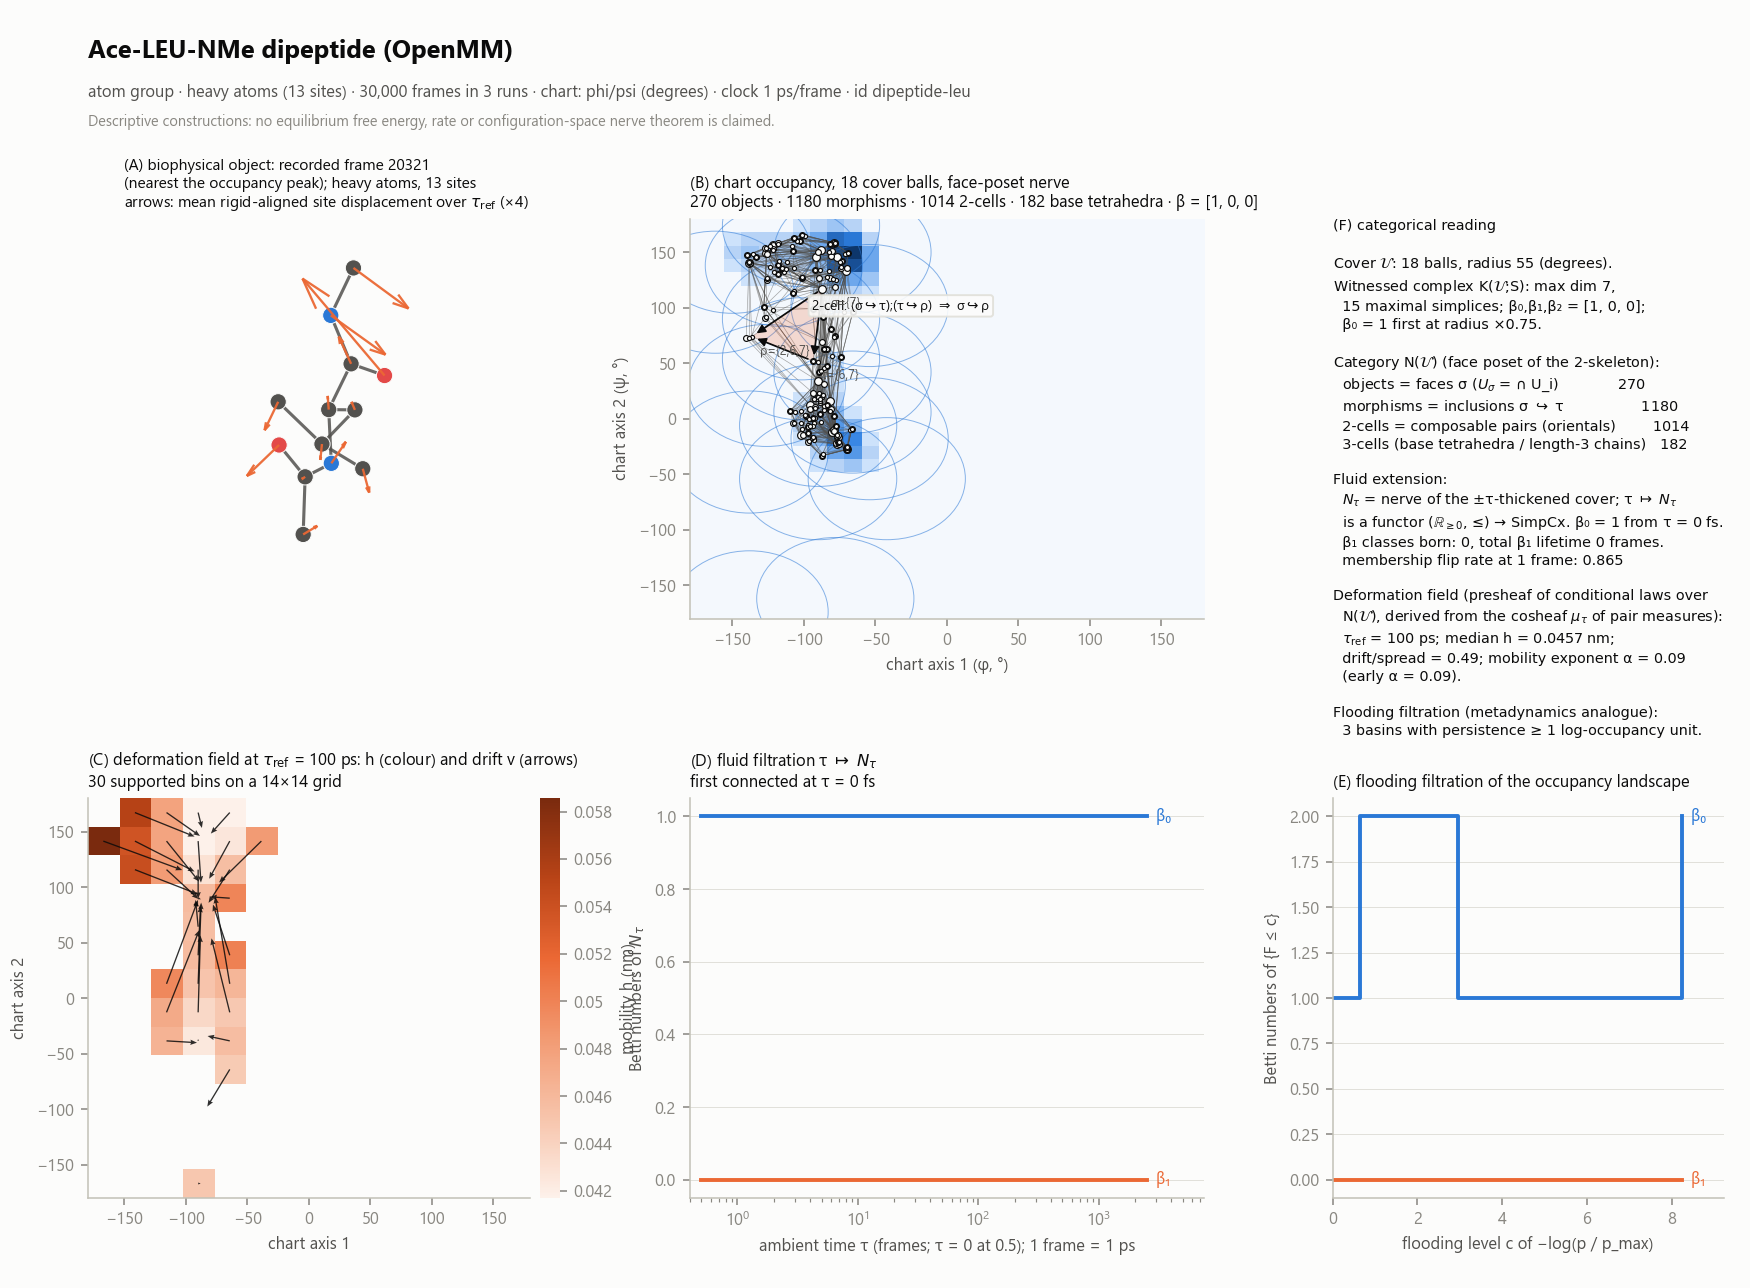
\includegraphics[width=\linewidth,height=.93\textheight,keepaspectratio]{systems/dipeptide-leu/plate.png}\caption{Ace-LEU-NMe dipeptide (OpenMM) (\texttt{dipeptide-leu}). Source: generate\_dipeptides.py (this repository).}\end{figure}\clearpage
\begin{figure}[H]\centering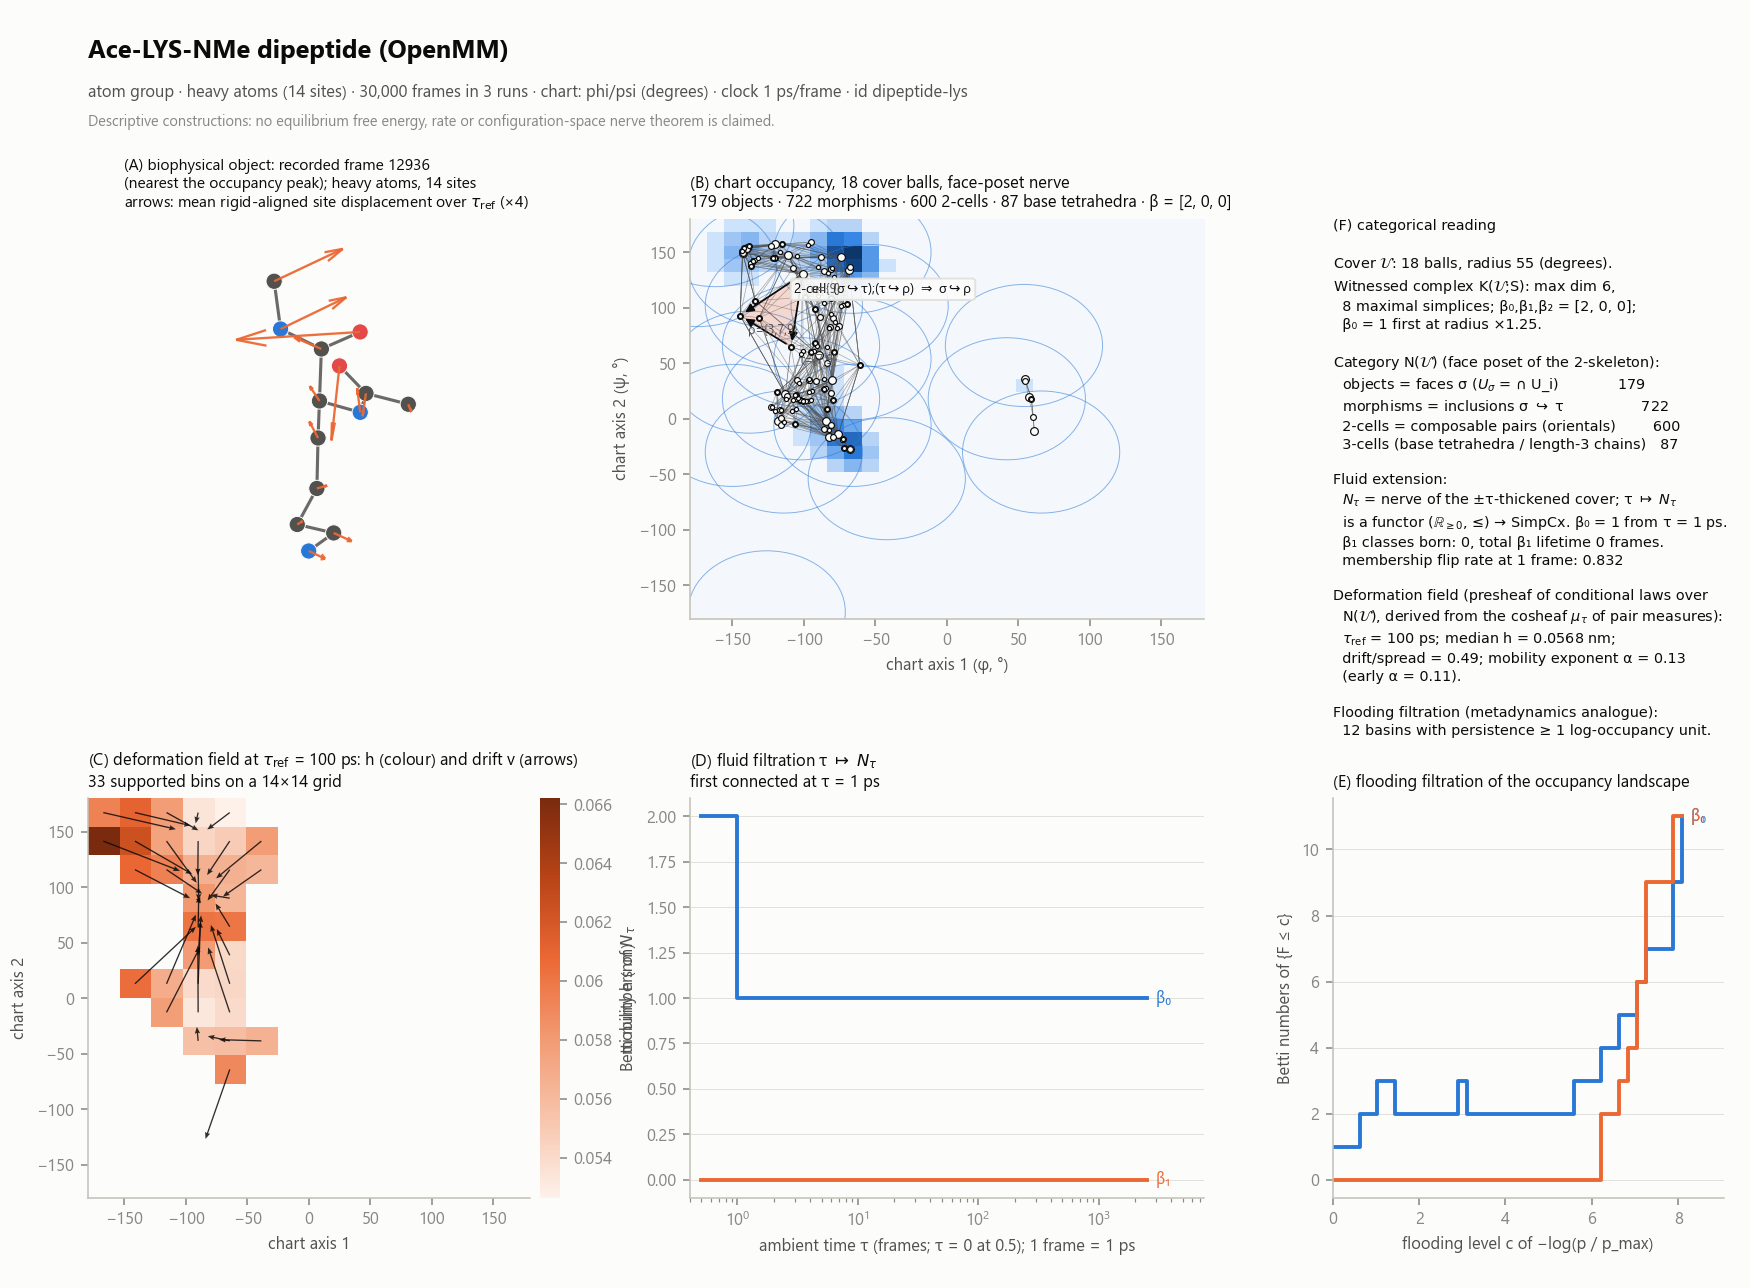
\includegraphics[width=\linewidth,height=.93\textheight,keepaspectratio]{systems/dipeptide-lys/plate.png}\caption{Ace-LYS-NMe dipeptide (OpenMM) (\texttt{dipeptide-lys}). Source: generate\_dipeptides.py (this repository).}\end{figure}\clearpage
\begin{figure}[H]\centering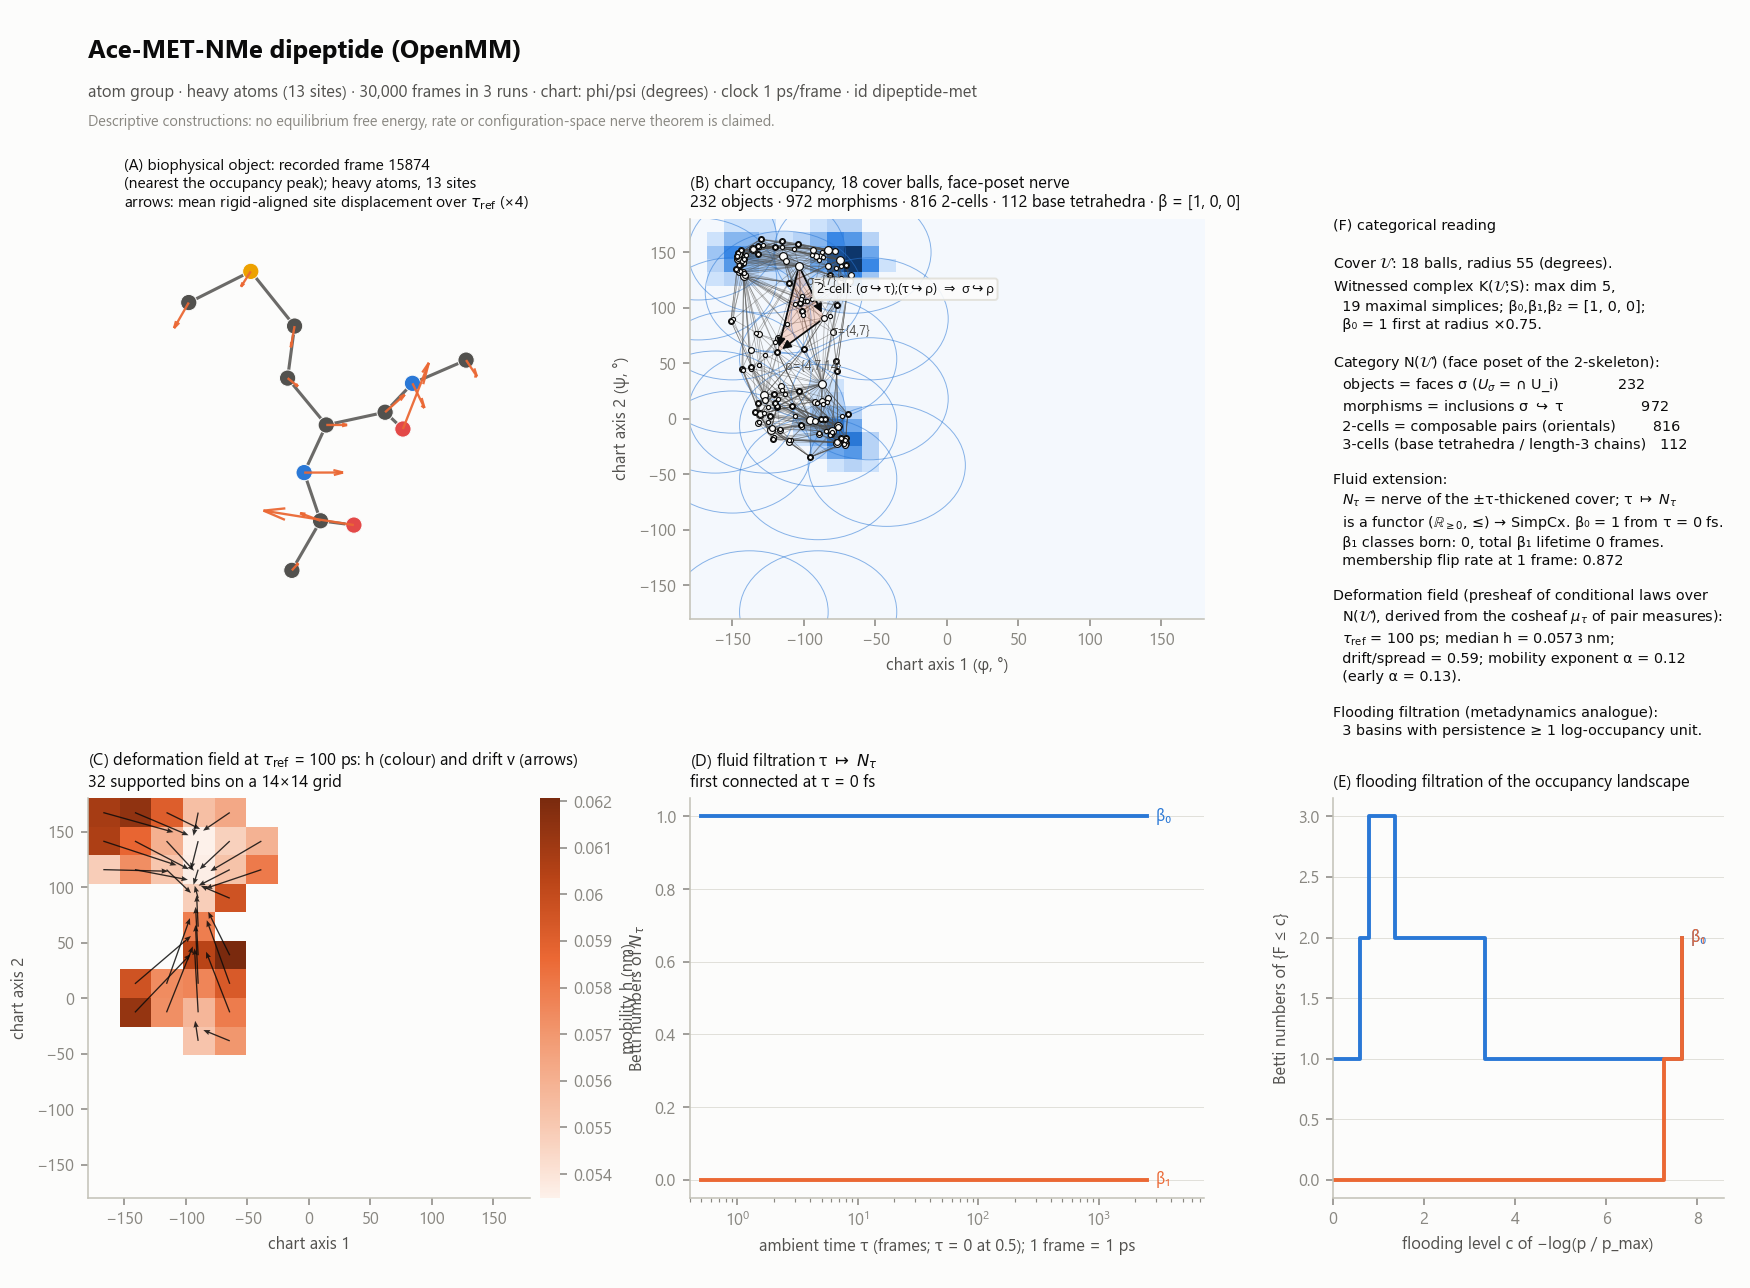
\includegraphics[width=\linewidth,height=.93\textheight,keepaspectratio]{systems/dipeptide-met/plate.png}\caption{Ace-MET-NMe dipeptide (OpenMM) (\texttt{dipeptide-met}). Source: generate\_dipeptides.py (this repository).}\end{figure}\clearpage
\begin{figure}[H]\centering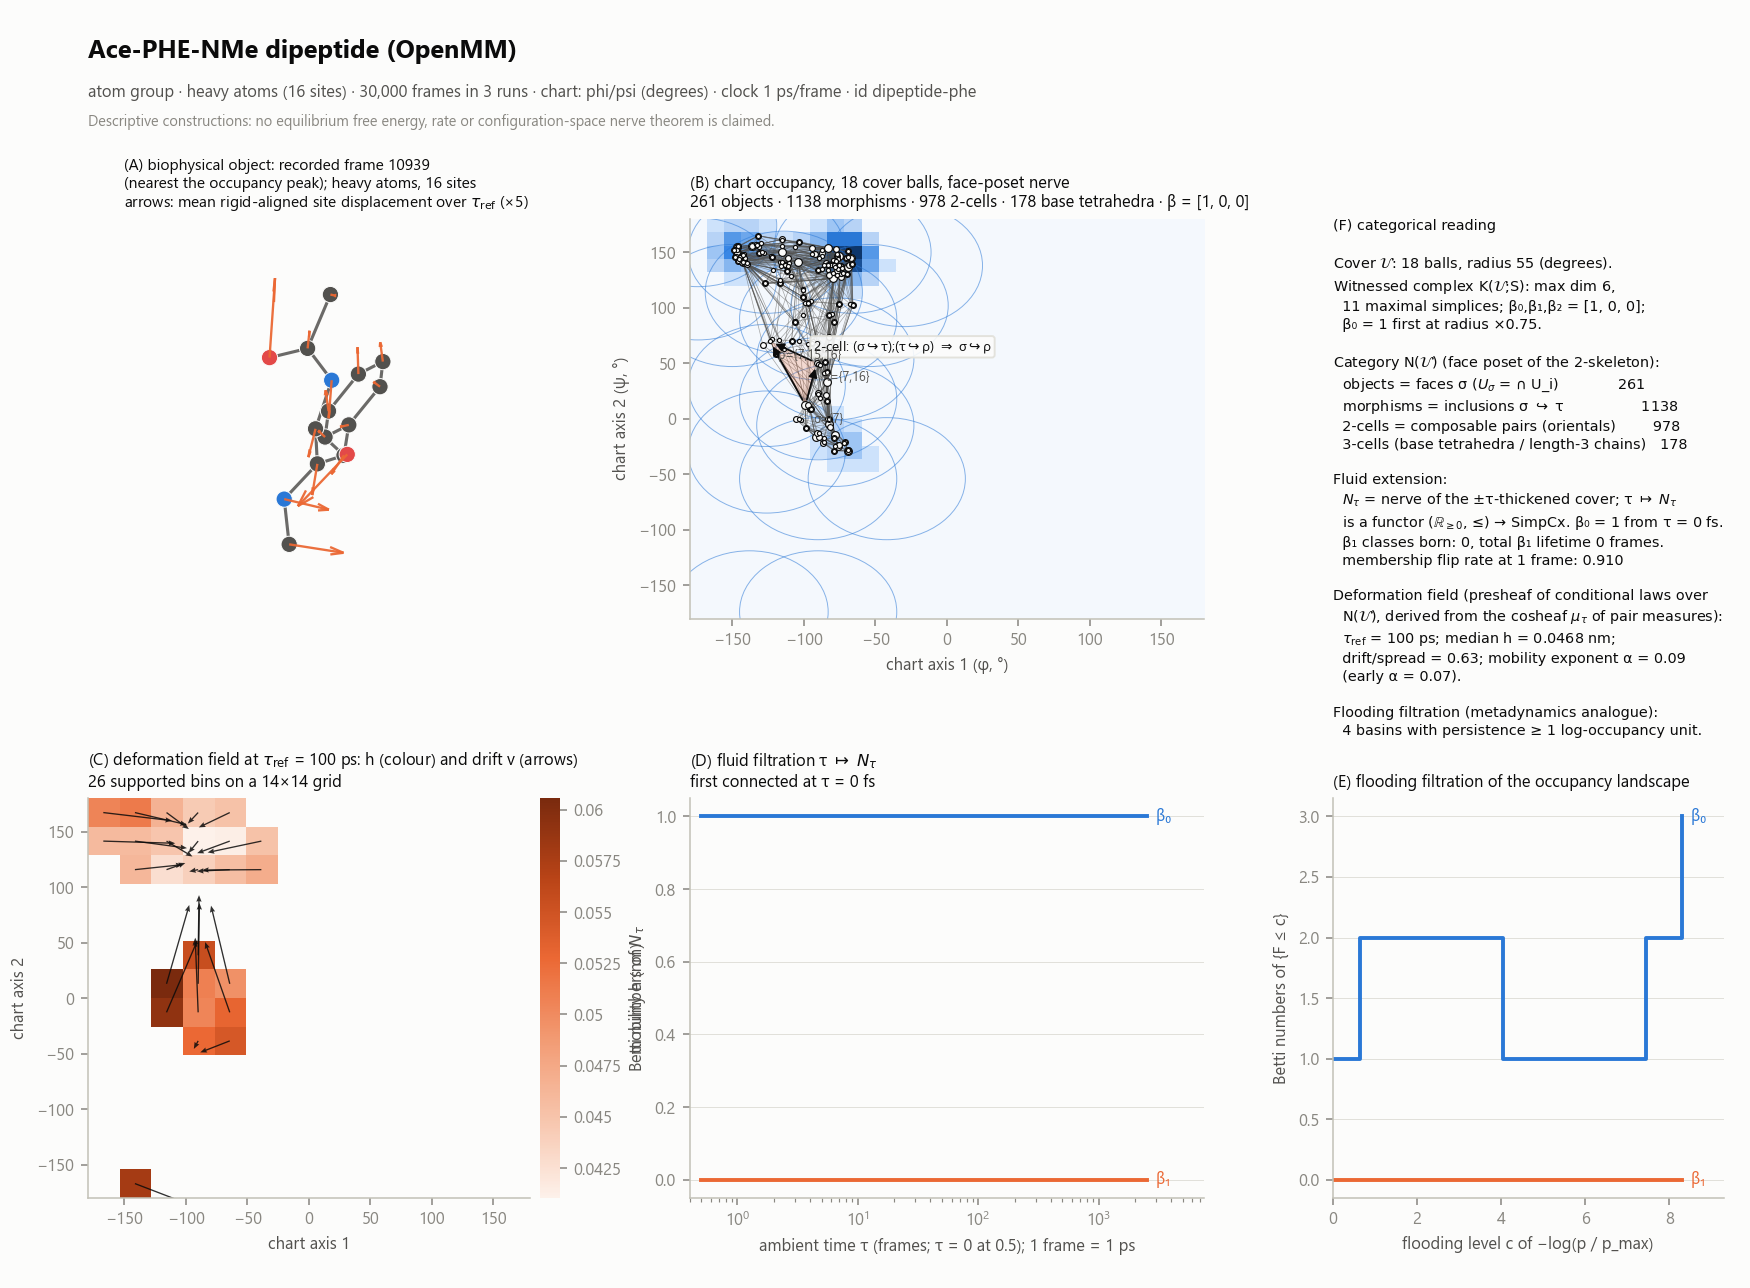
\includegraphics[width=\linewidth,height=.93\textheight,keepaspectratio]{systems/dipeptide-phe/plate.png}\caption{Ace-PHE-NMe dipeptide (OpenMM) (\texttt{dipeptide-phe}). Source: generate\_dipeptides.py (this repository).}\end{figure}\clearpage
\begin{figure}[H]\centering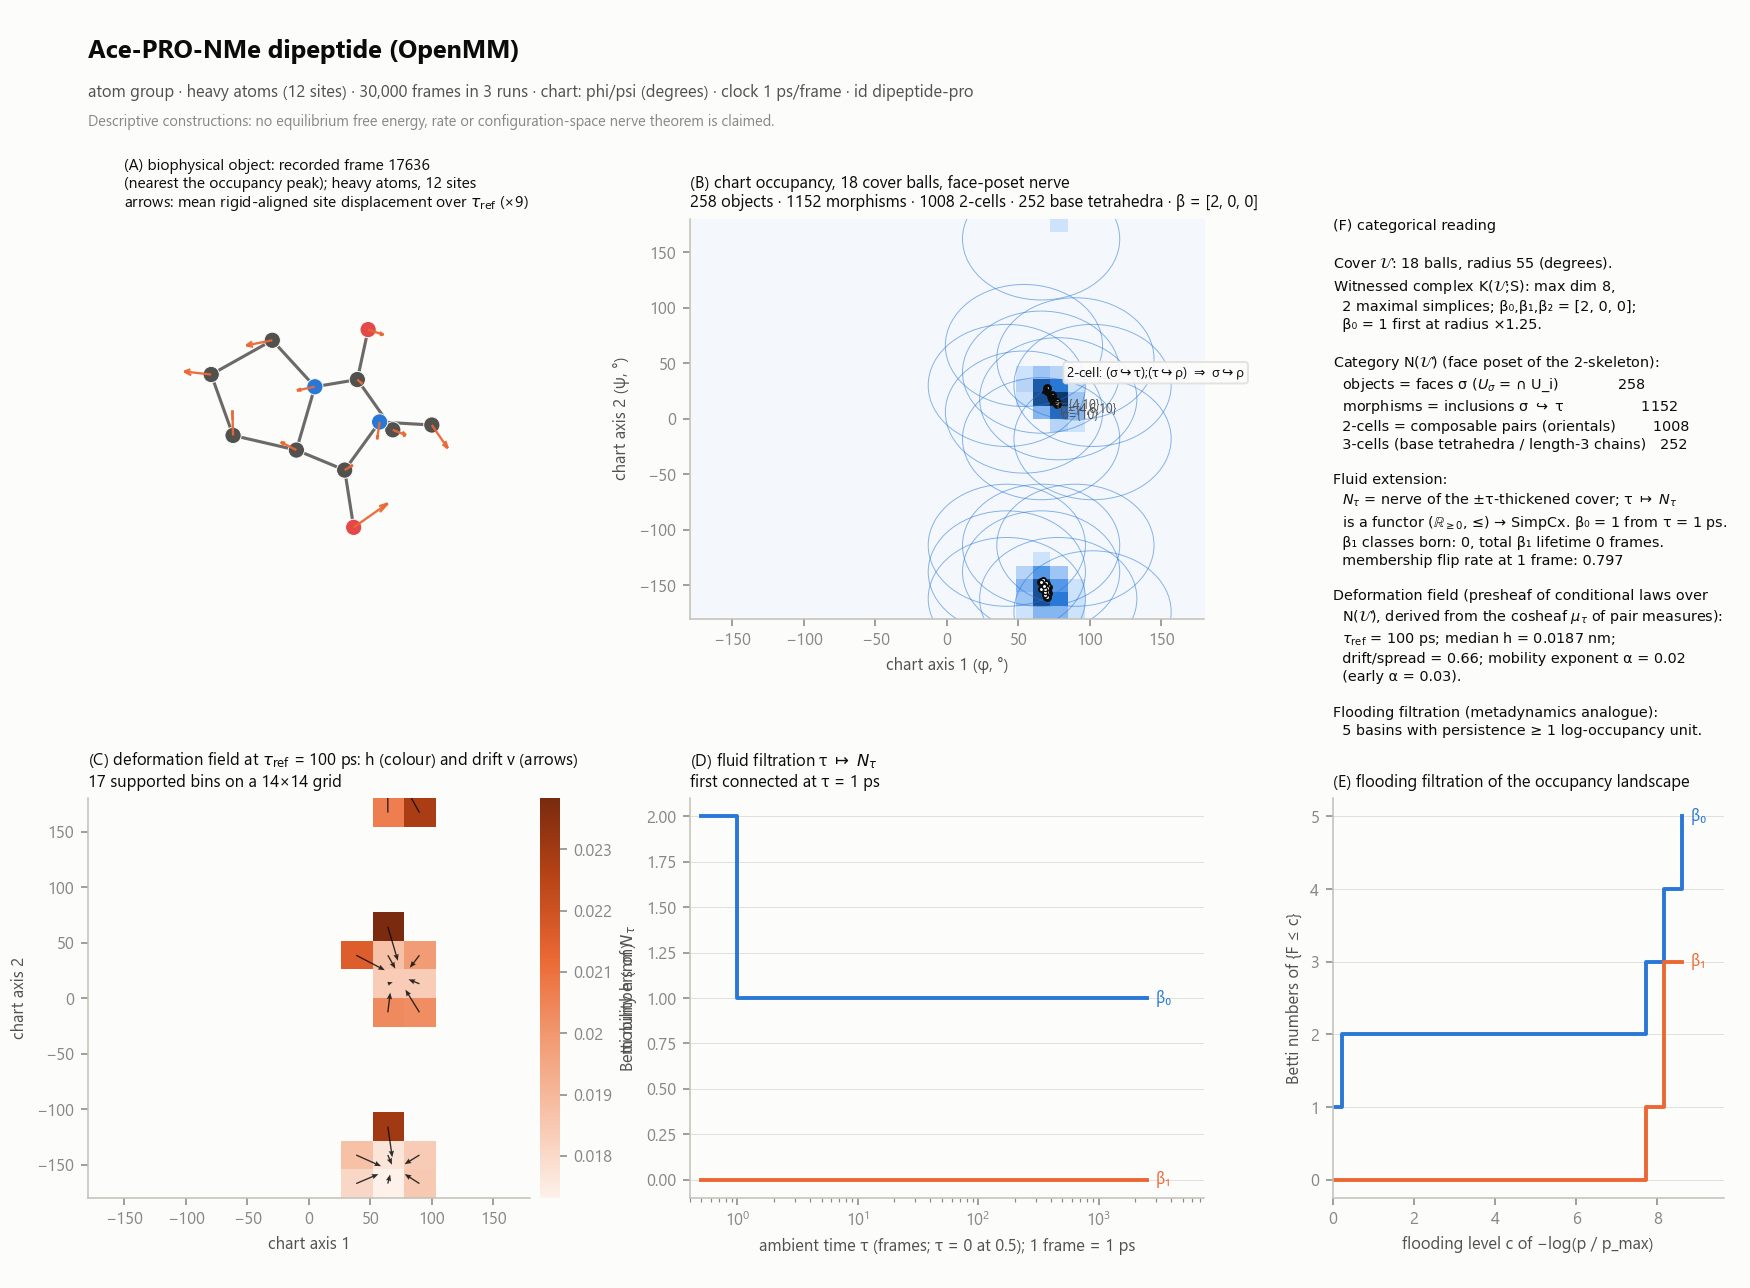
\includegraphics[width=\linewidth,height=.93\textheight,keepaspectratio]{systems/dipeptide-pro/plate.png}\caption{Ace-PRO-NMe dipeptide (OpenMM) (\texttt{dipeptide-pro}). Source: generate\_dipeptides.py (this repository).}\end{figure}\clearpage
\begin{figure}[H]\centering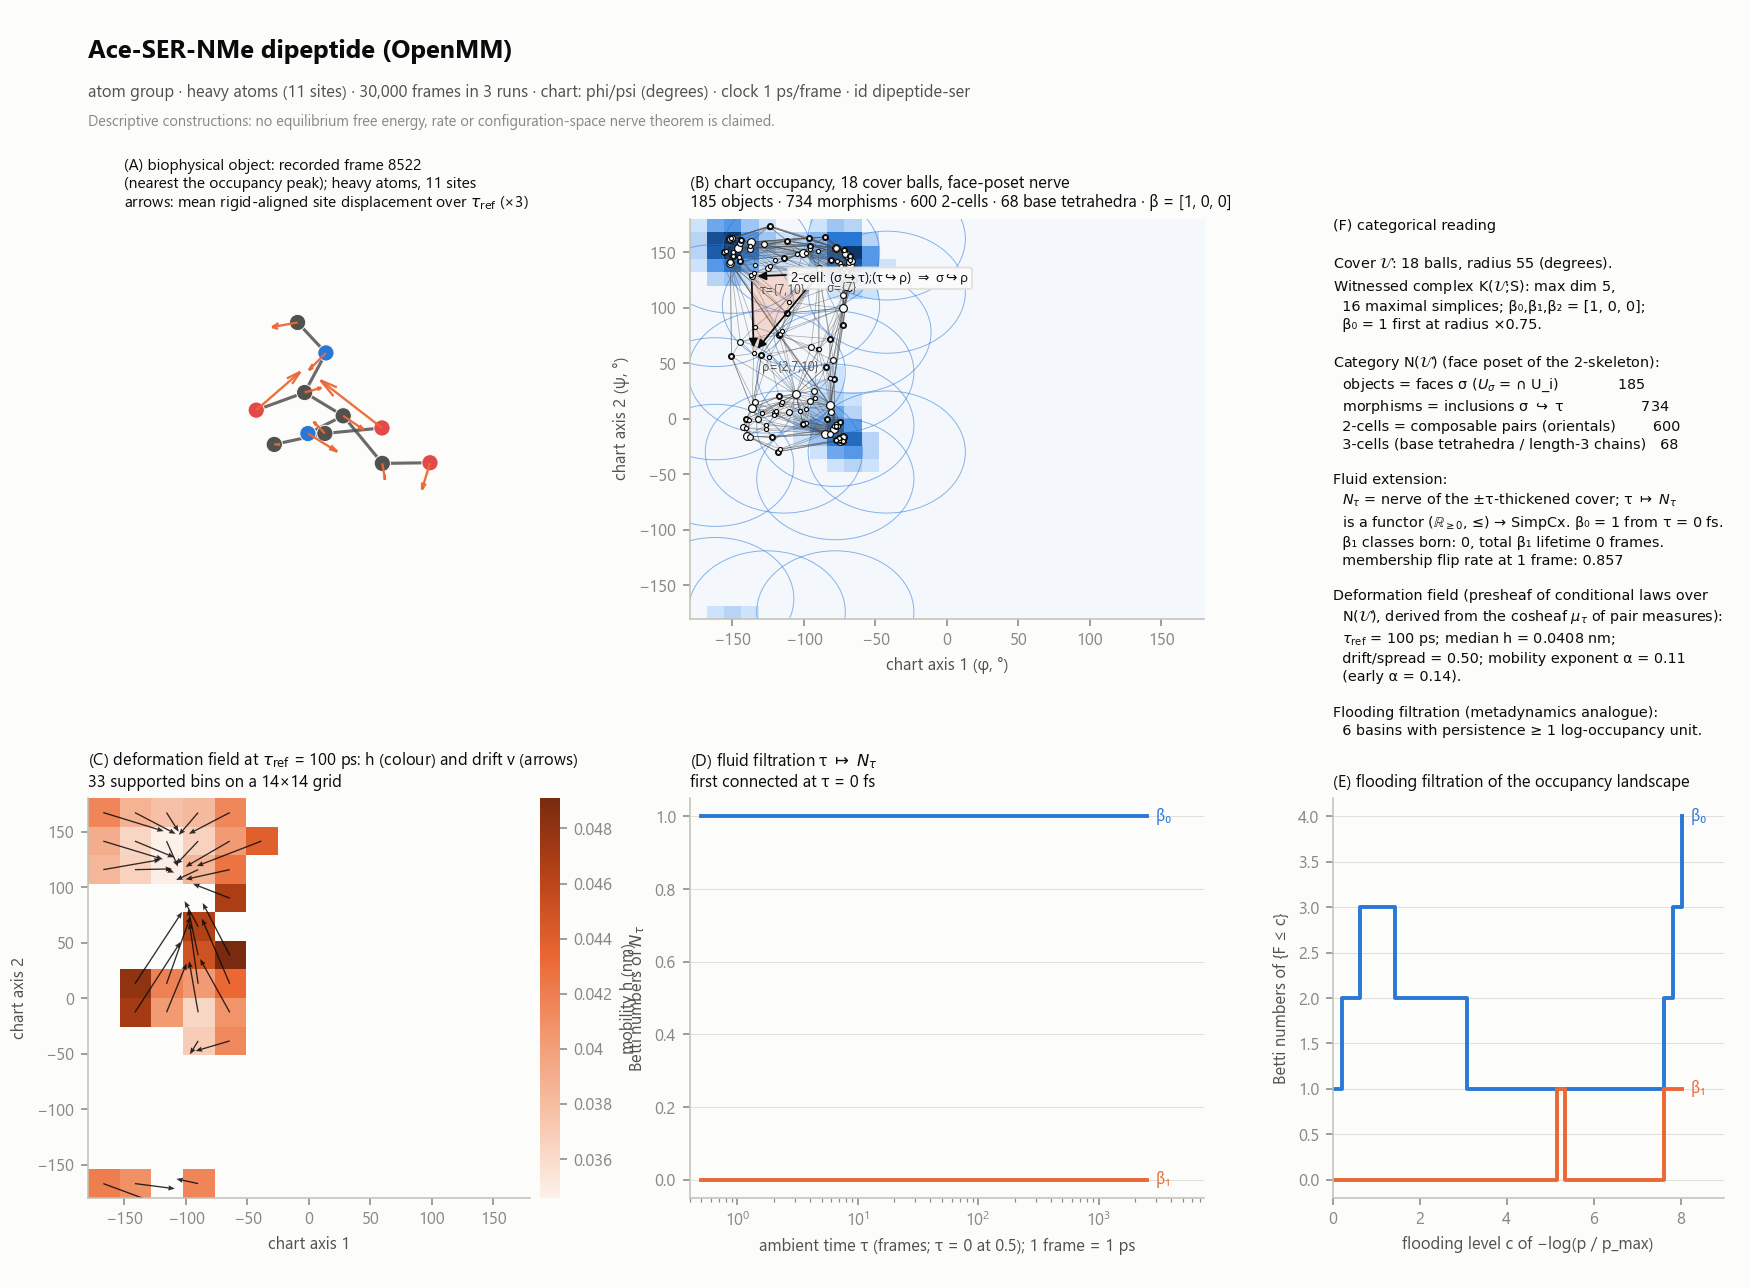
\includegraphics[width=\linewidth,height=.93\textheight,keepaspectratio]{systems/dipeptide-ser/plate.png}\caption{Ace-SER-NMe dipeptide (OpenMM) (\texttt{dipeptide-ser}). Source: generate\_dipeptides.py (this repository).}\end{figure}\clearpage
\begin{figure}[H]\centering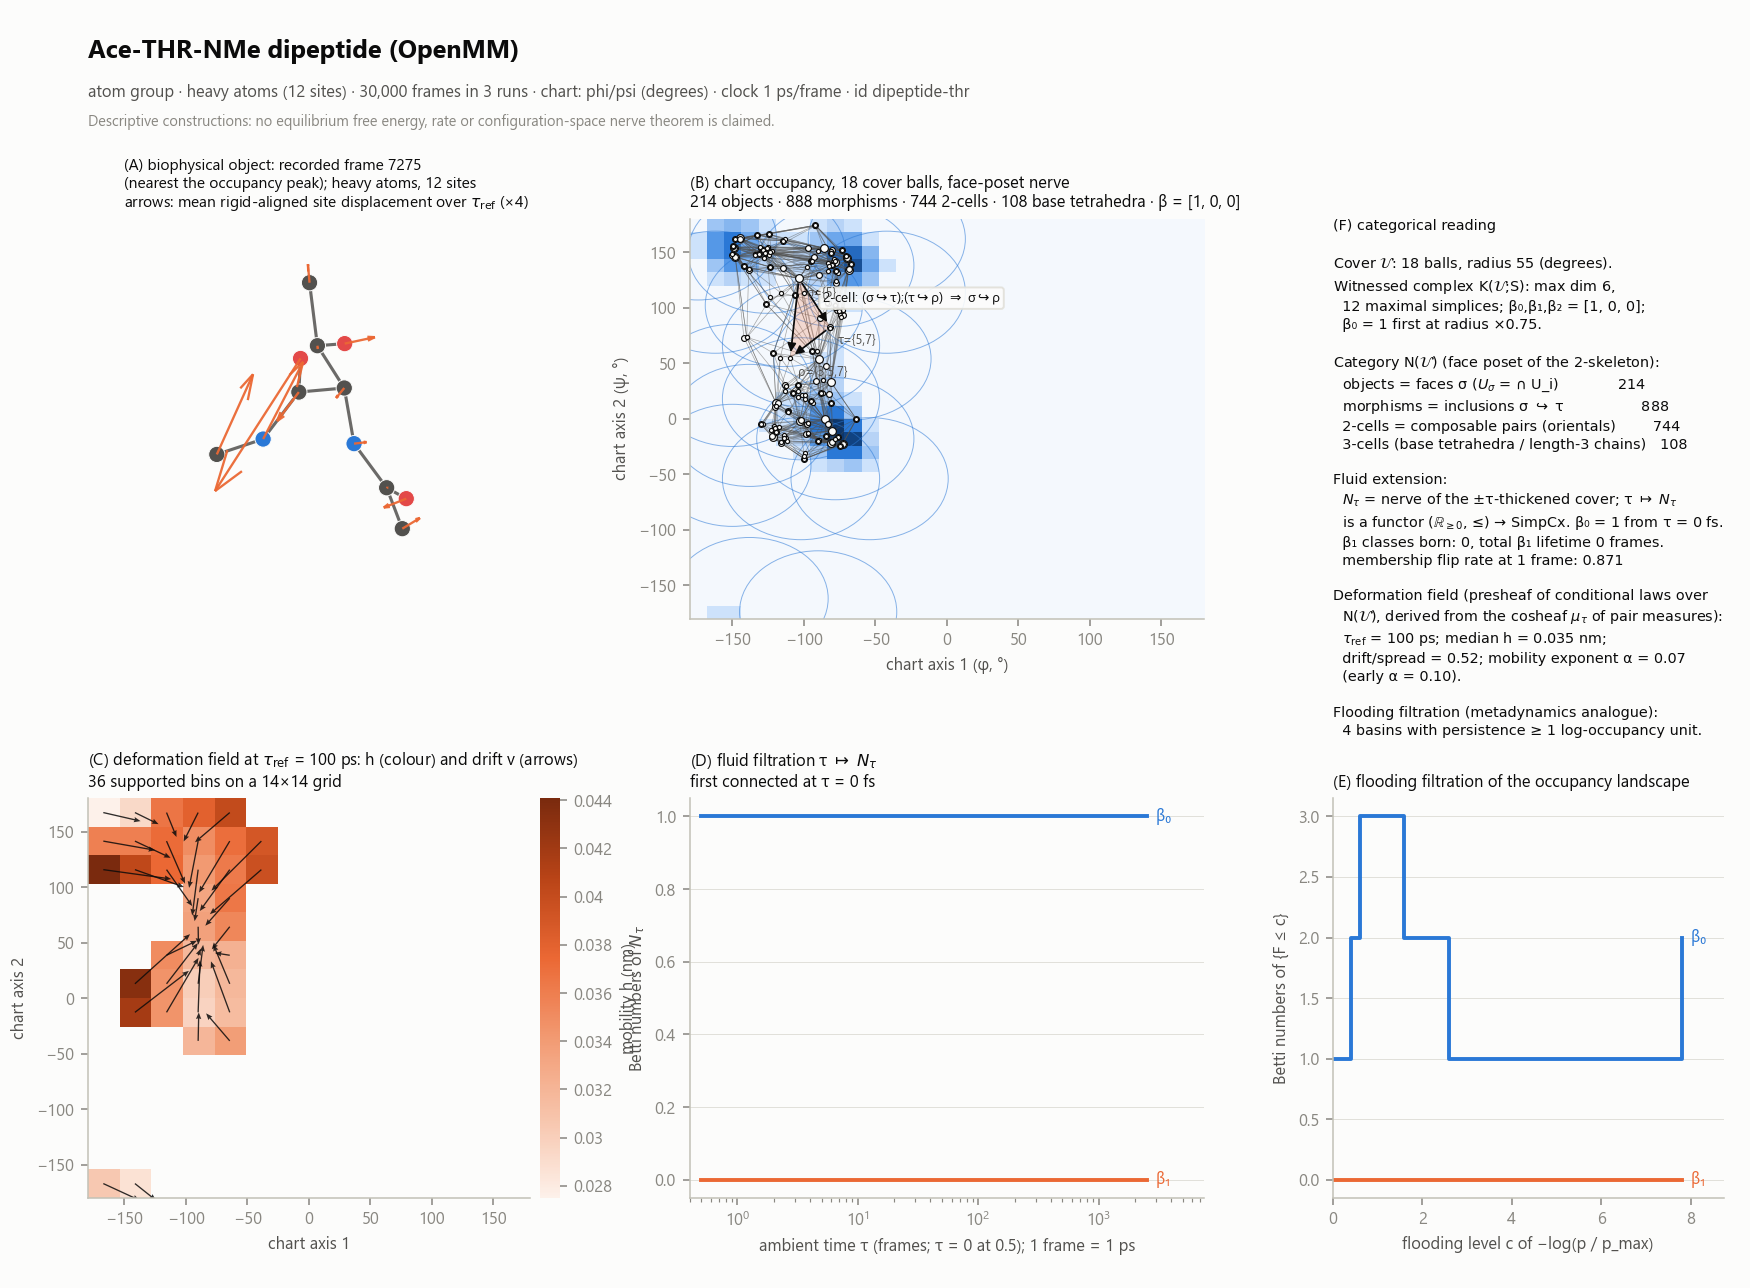
\includegraphics[width=\linewidth,height=.93\textheight,keepaspectratio]{systems/dipeptide-thr/plate.png}\caption{Ace-THR-NMe dipeptide (OpenMM) (\texttt{dipeptide-thr}). Source: generate\_dipeptides.py (this repository).}\end{figure}\clearpage
\begin{figure}[H]\centering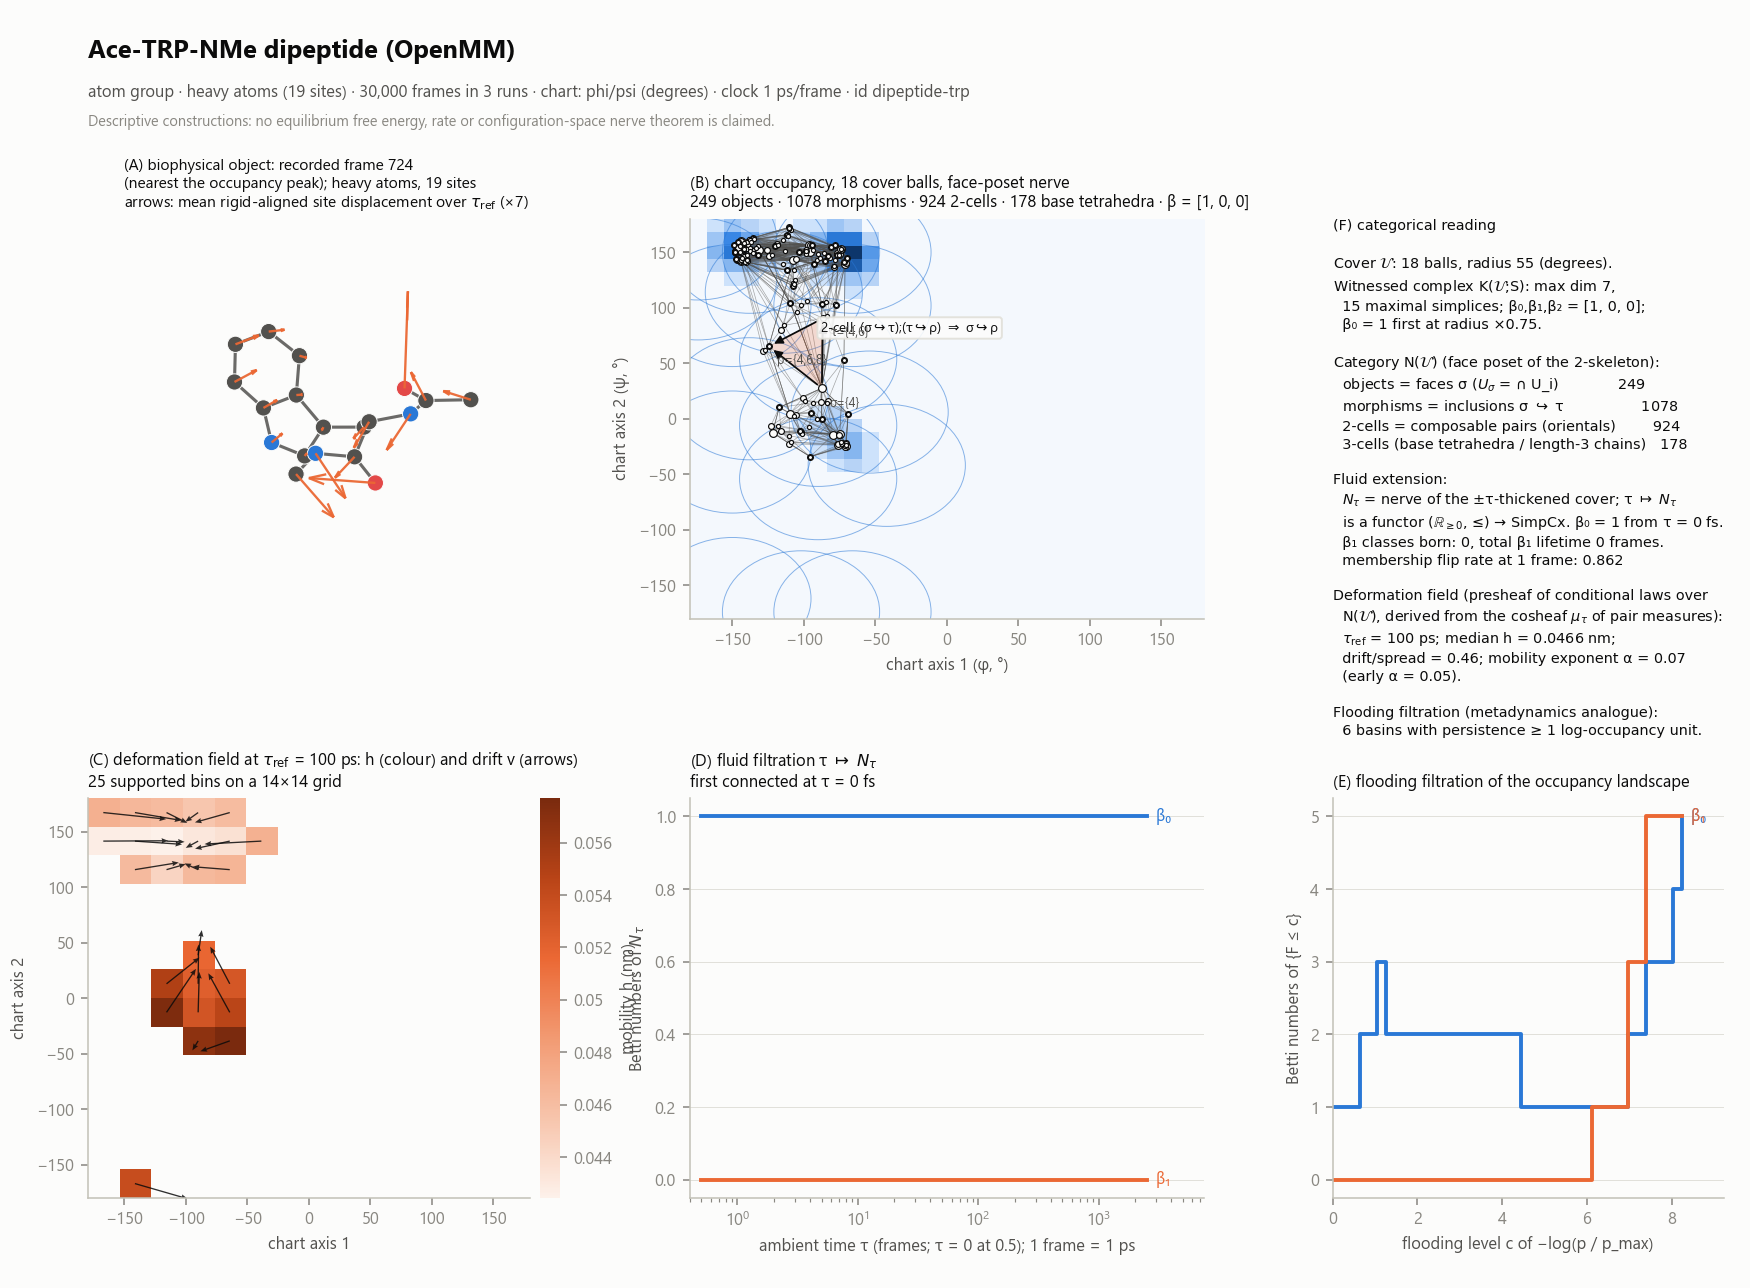
\includegraphics[width=\linewidth,height=.93\textheight,keepaspectratio]{systems/dipeptide-trp/plate.png}\caption{Ace-TRP-NMe dipeptide (OpenMM) (\texttt{dipeptide-trp}). Source: generate\_dipeptides.py (this repository).}\end{figure}\clearpage
\begin{figure}[H]\centering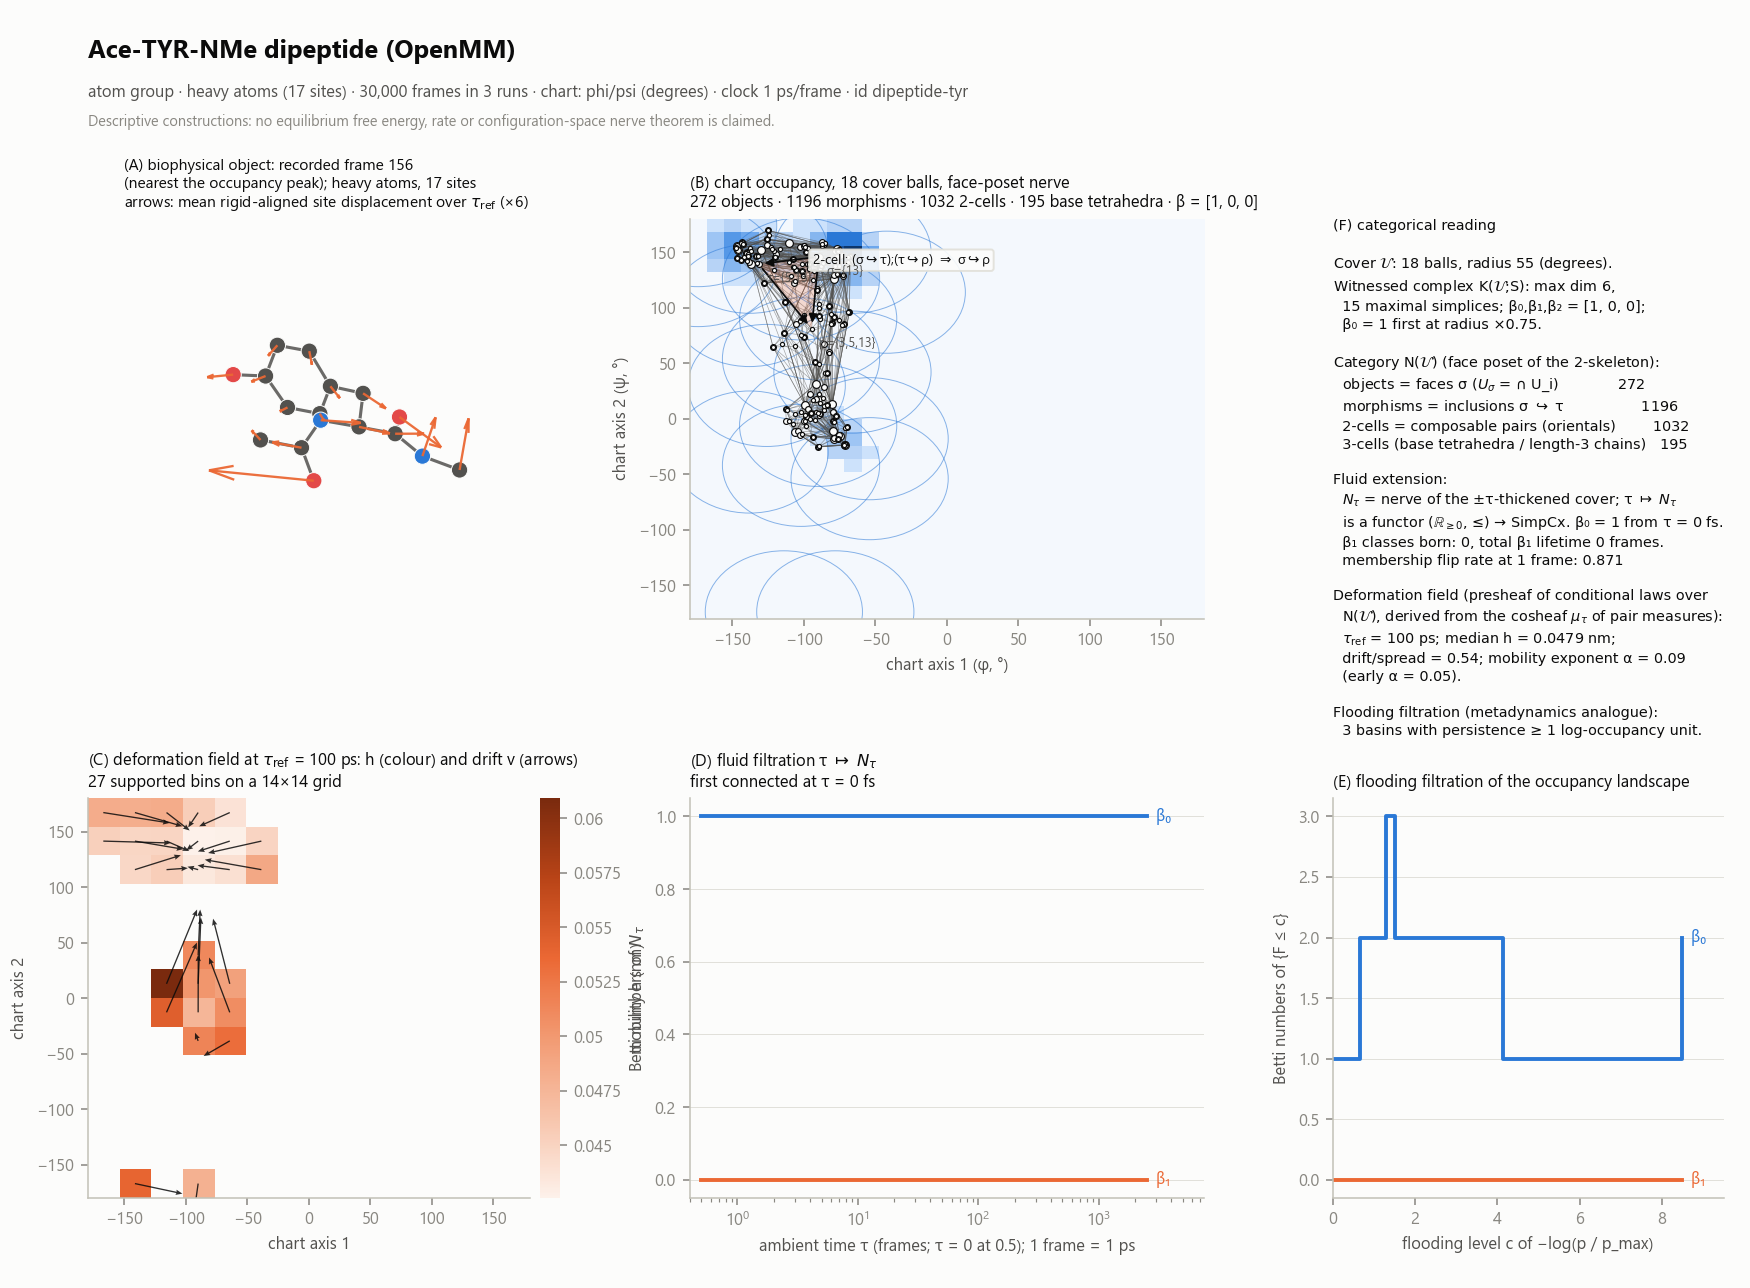
\includegraphics[width=\linewidth,height=.93\textheight,keepaspectratio]{systems/dipeptide-tyr/plate.png}\caption{Ace-TYR-NMe dipeptide (OpenMM) (\texttt{dipeptide-tyr}). Source: generate\_dipeptides.py (this repository).}\end{figure}\clearpage
\begin{figure}[H]\centering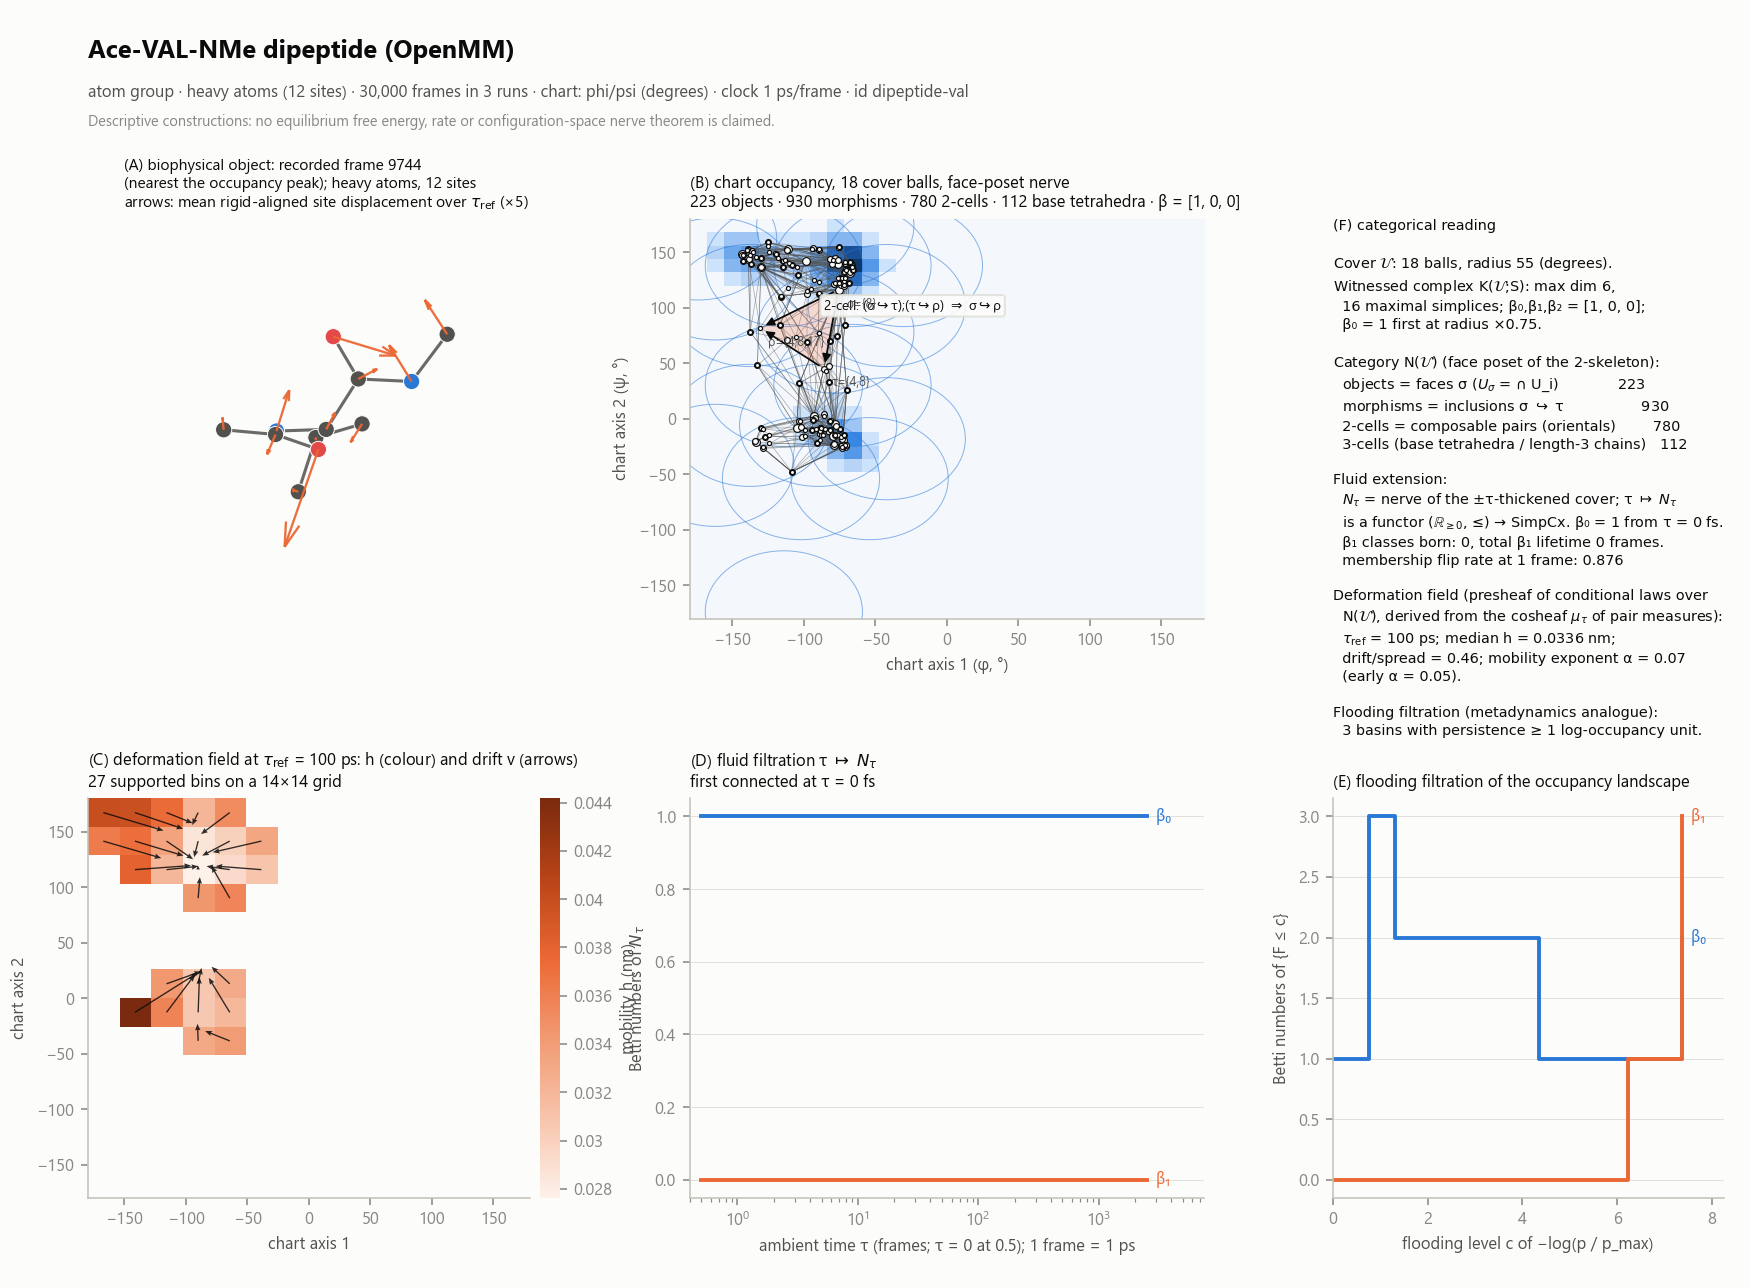
\includegraphics[width=\linewidth,height=.93\textheight,keepaspectratio]{systems/dipeptide-val/plate.png}\caption{Ace-VAL-NMe dipeptide (OpenMM) (\texttt{dipeptide-val}). Source: generate\_dipeptides.py (this repository).}\end{figure}\clearpage
\begin{figure}[H]\centering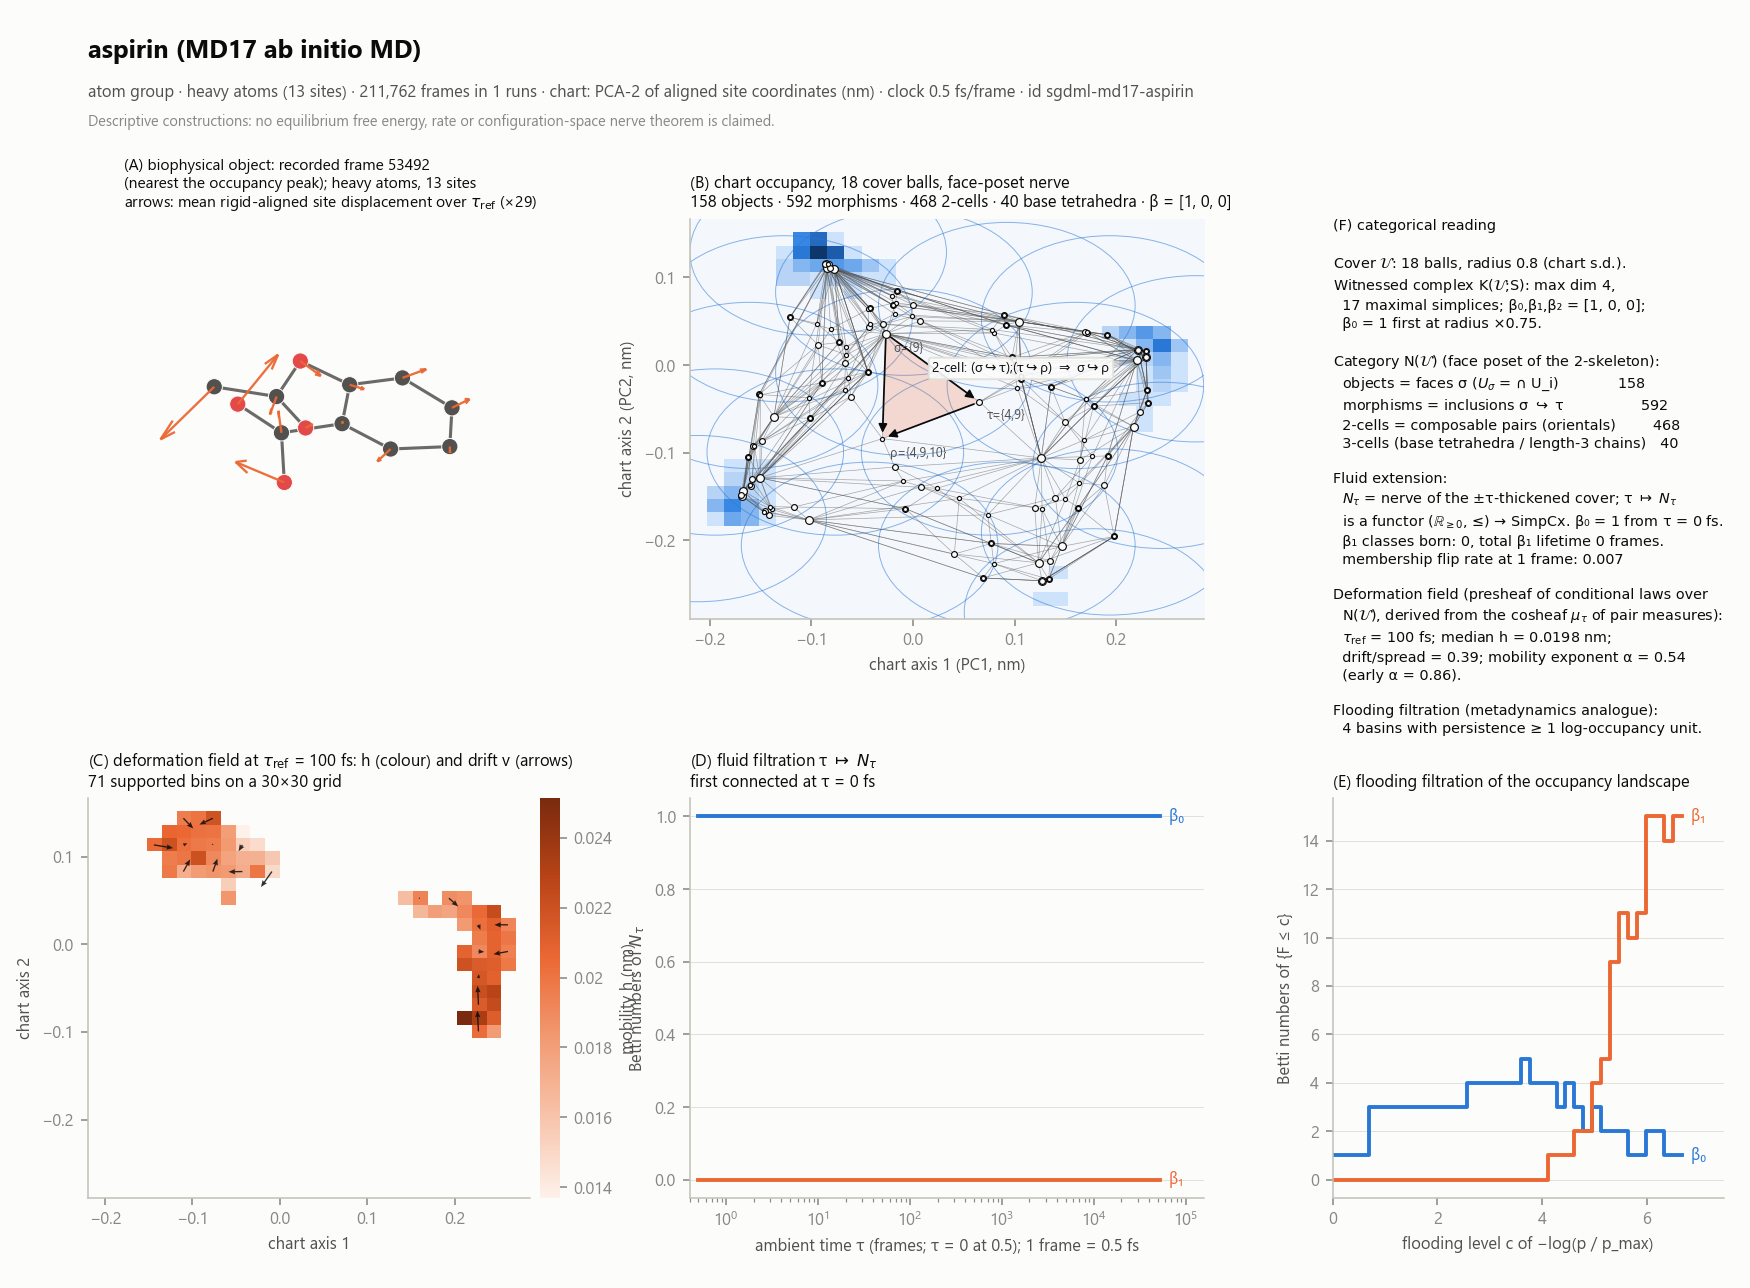
\includegraphics[width=\linewidth,height=.93\textheight,keepaspectratio]{systems/sgdml-md17-aspirin/plate.png}\caption{aspirin (MD17 ab initio MD) (\texttt{sgdml-md17-aspirin}). Source: https://www.quantum-machine.org/gdml/data/npz/md17\_aspirin.npz.}\end{figure}\clearpage
\begin{figure}[H]\centering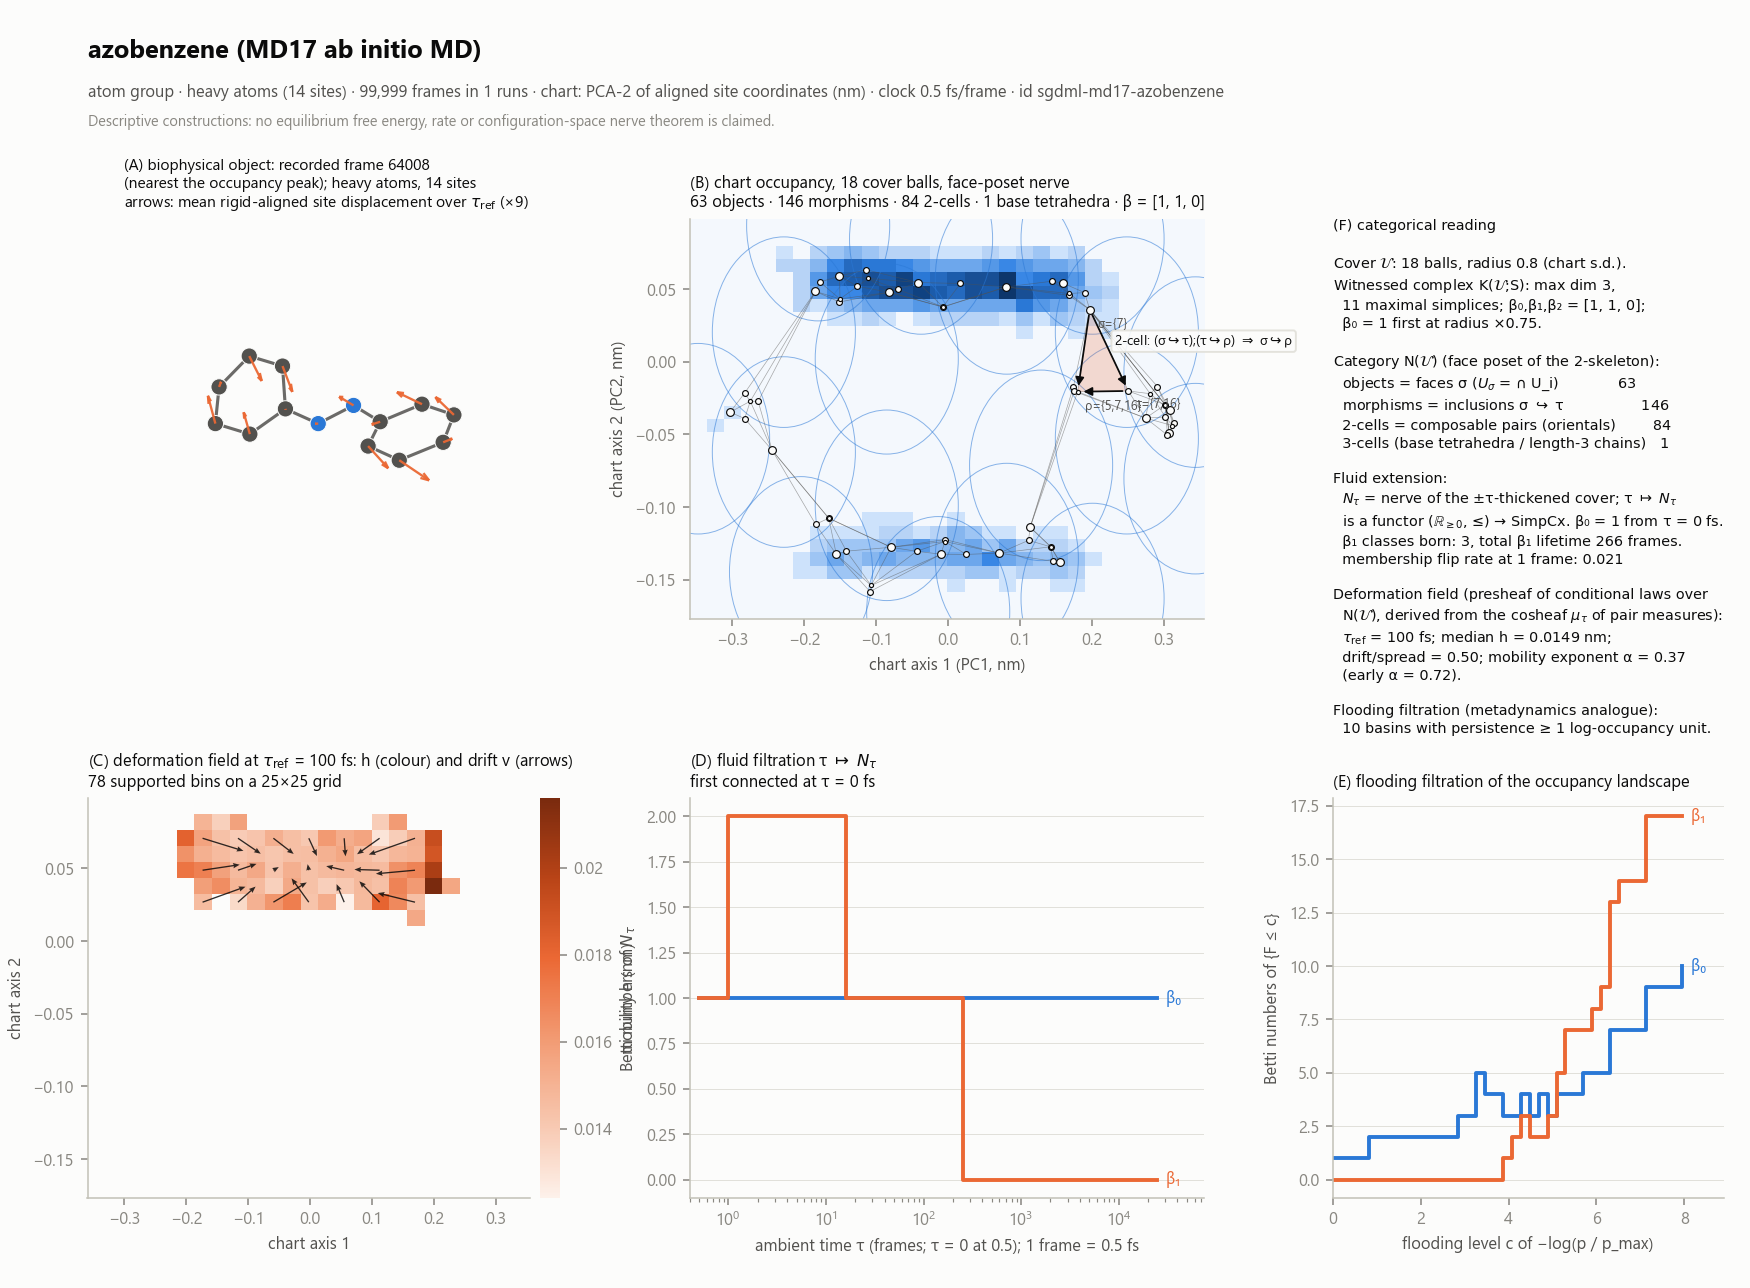
\includegraphics[width=\linewidth,height=.93\textheight,keepaspectratio]{systems/sgdml-md17-azobenzene/plate.png}\caption{azobenzene (MD17 ab initio MD) (\texttt{sgdml-md17-azobenzene}). Source: https://www.quantum-machine.org/gdml/data/npz/azobenzene\_dft.npz.}\end{figure}\clearpage
\begin{figure}[H]\centering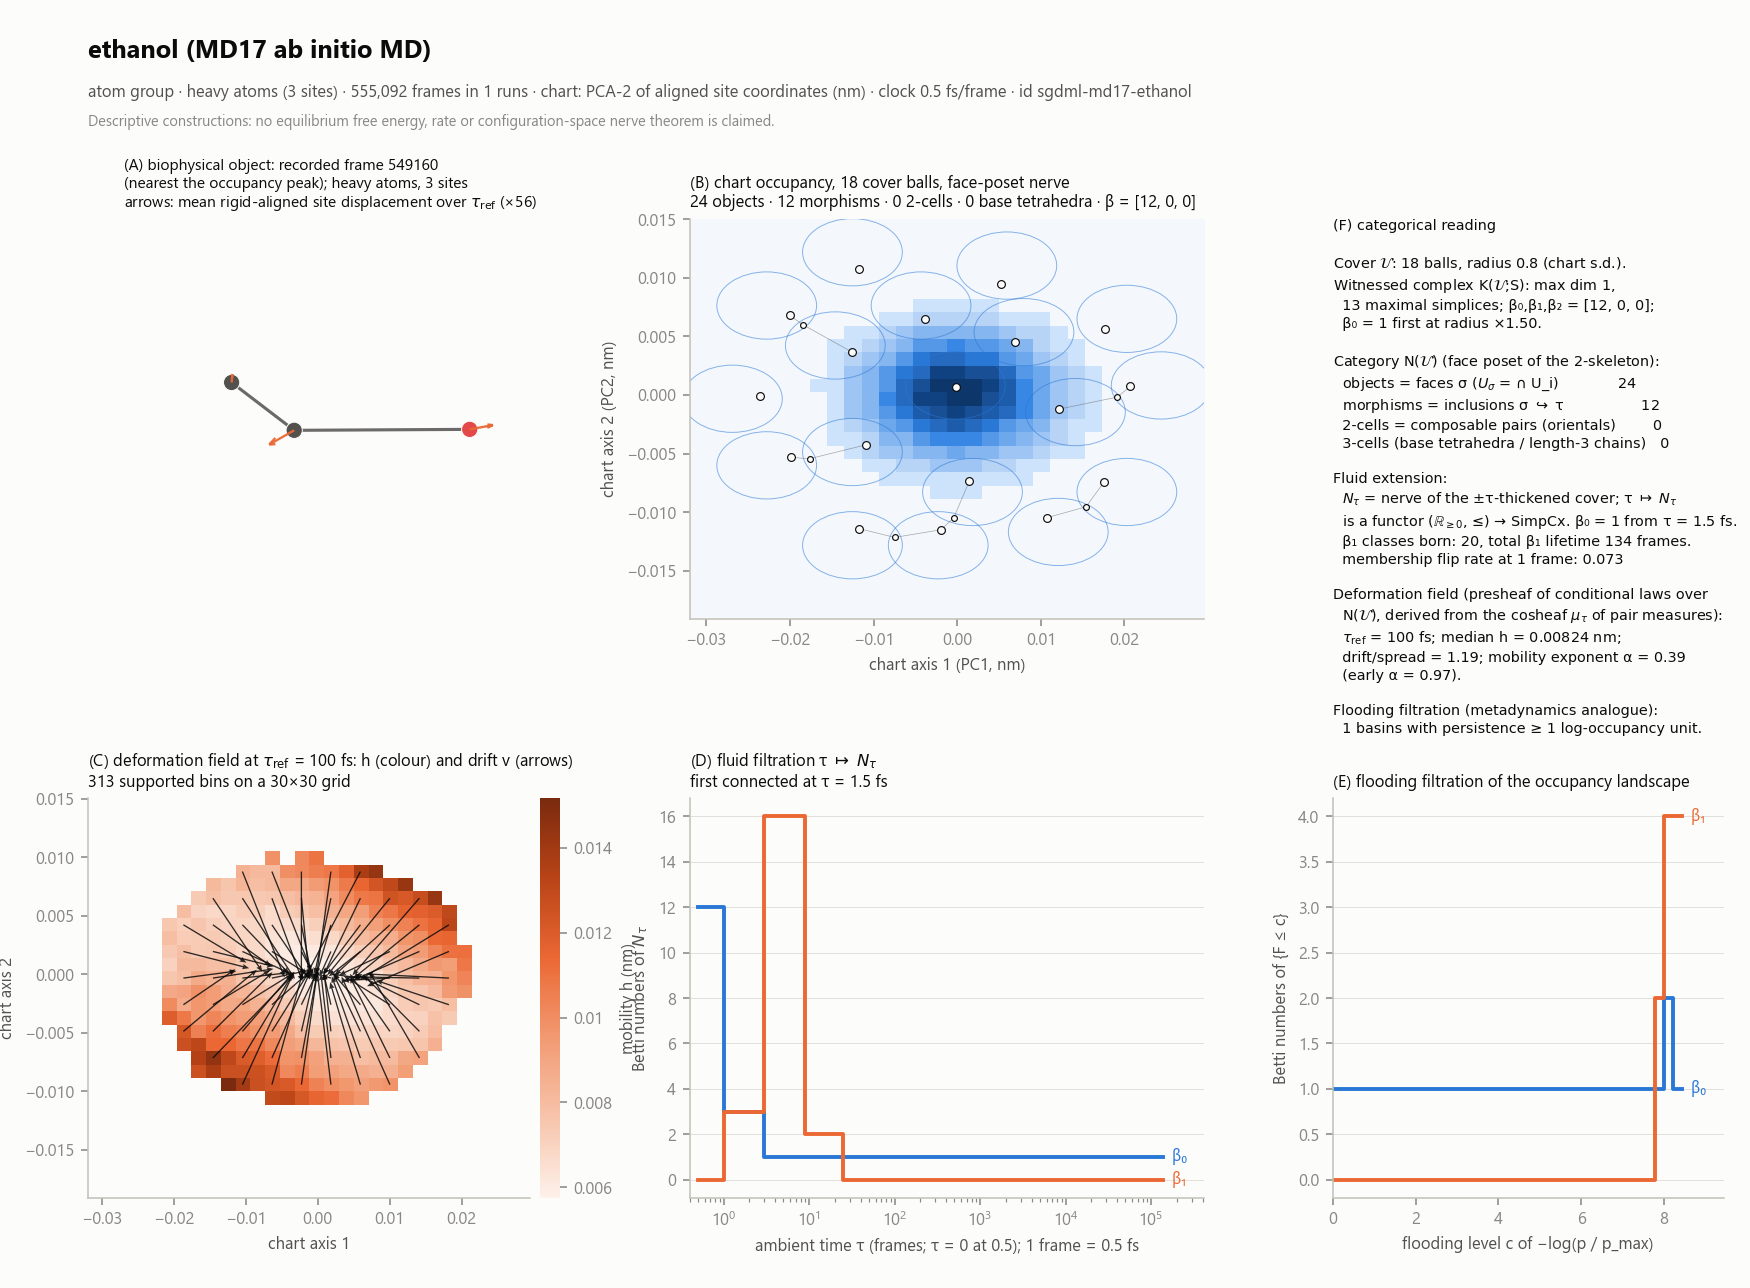
\includegraphics[width=\linewidth,height=.93\textheight,keepaspectratio]{systems/sgdml-md17-ethanol/plate.png}\caption{ethanol (MD17 ab initio MD) (\texttt{sgdml-md17-ethanol}). Source: https://www.quantum-machine.org/gdml/data/npz/md17\_ethanol.npz.}\end{figure}\clearpage
\begin{figure}[H]\centering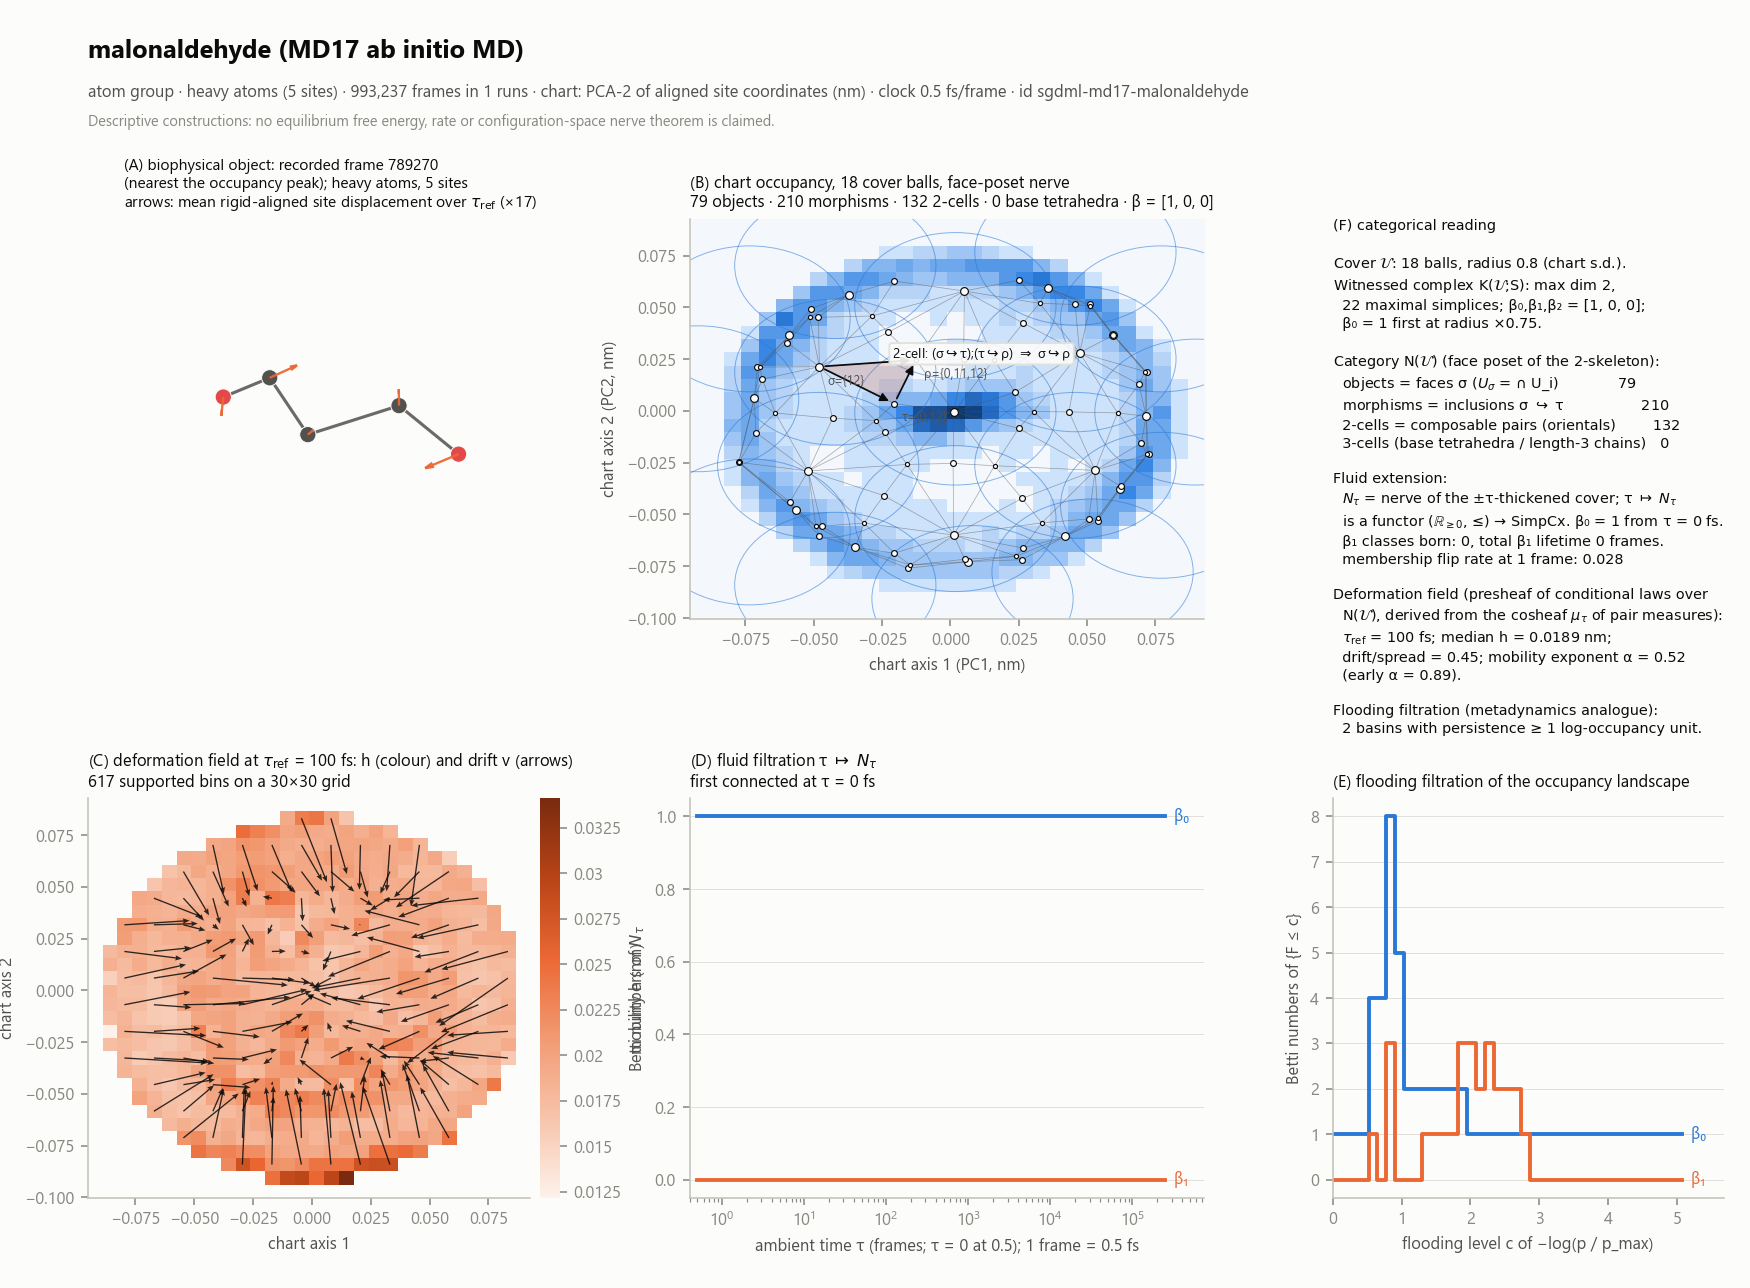
\includegraphics[width=\linewidth,height=.93\textheight,keepaspectratio]{systems/sgdml-md17-malonaldehyde/plate.png}\caption{malonaldehyde (MD17 ab initio MD) (\texttt{sgdml-md17-malonaldehyde}). Source: https://www.quantum-machine.org/gdml/data/npz/md17\_malonaldehyde.npz.}\end{figure}\clearpage
\begin{figure}[H]\centering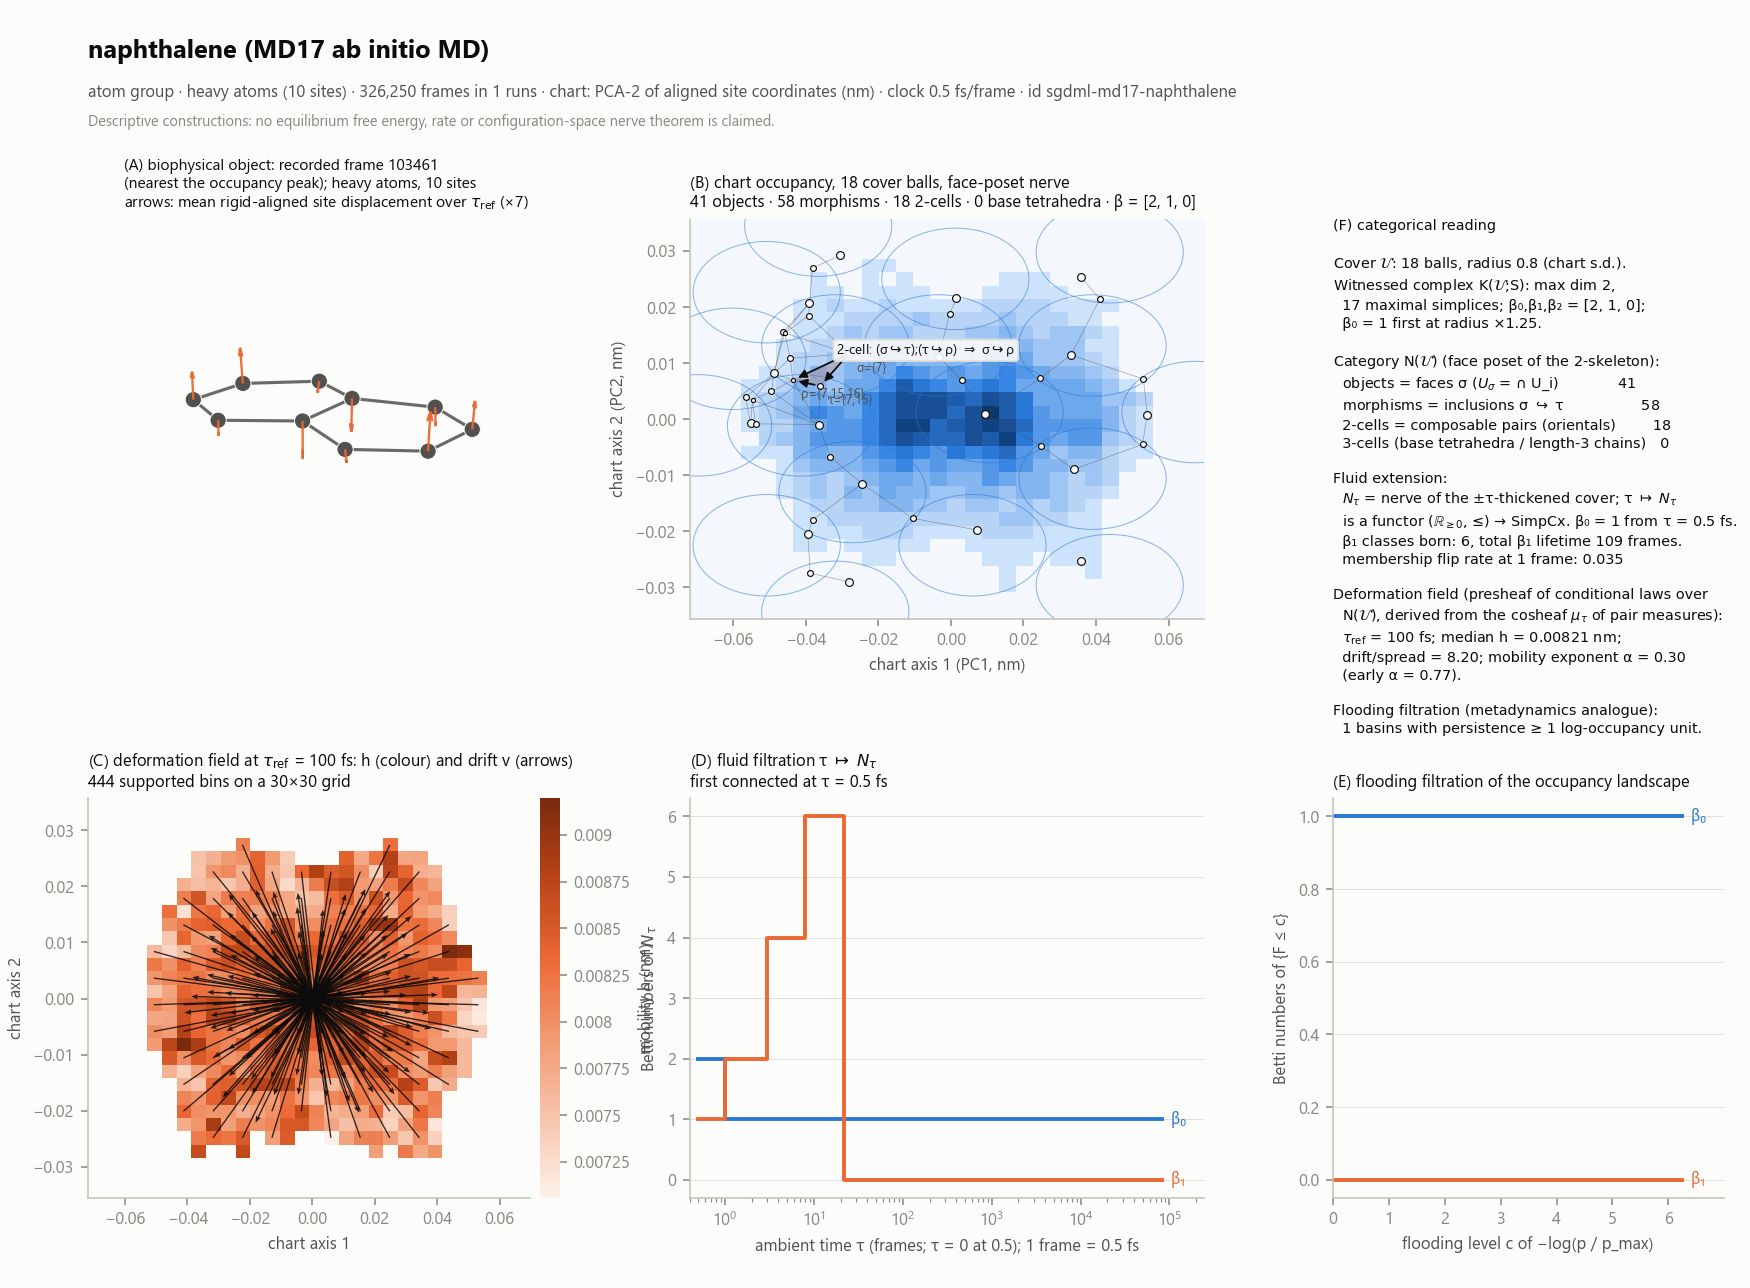
\includegraphics[width=\linewidth,height=.93\textheight,keepaspectratio]{systems/sgdml-md17-naphthalene/plate.png}\caption{naphthalene (MD17 ab initio MD) (\texttt{sgdml-md17-naphthalene}). Source: https://www.quantum-machine.org/gdml/data/npz/md17\_naphthalene.npz.}\end{figure}\clearpage
\begin{figure}[H]\centering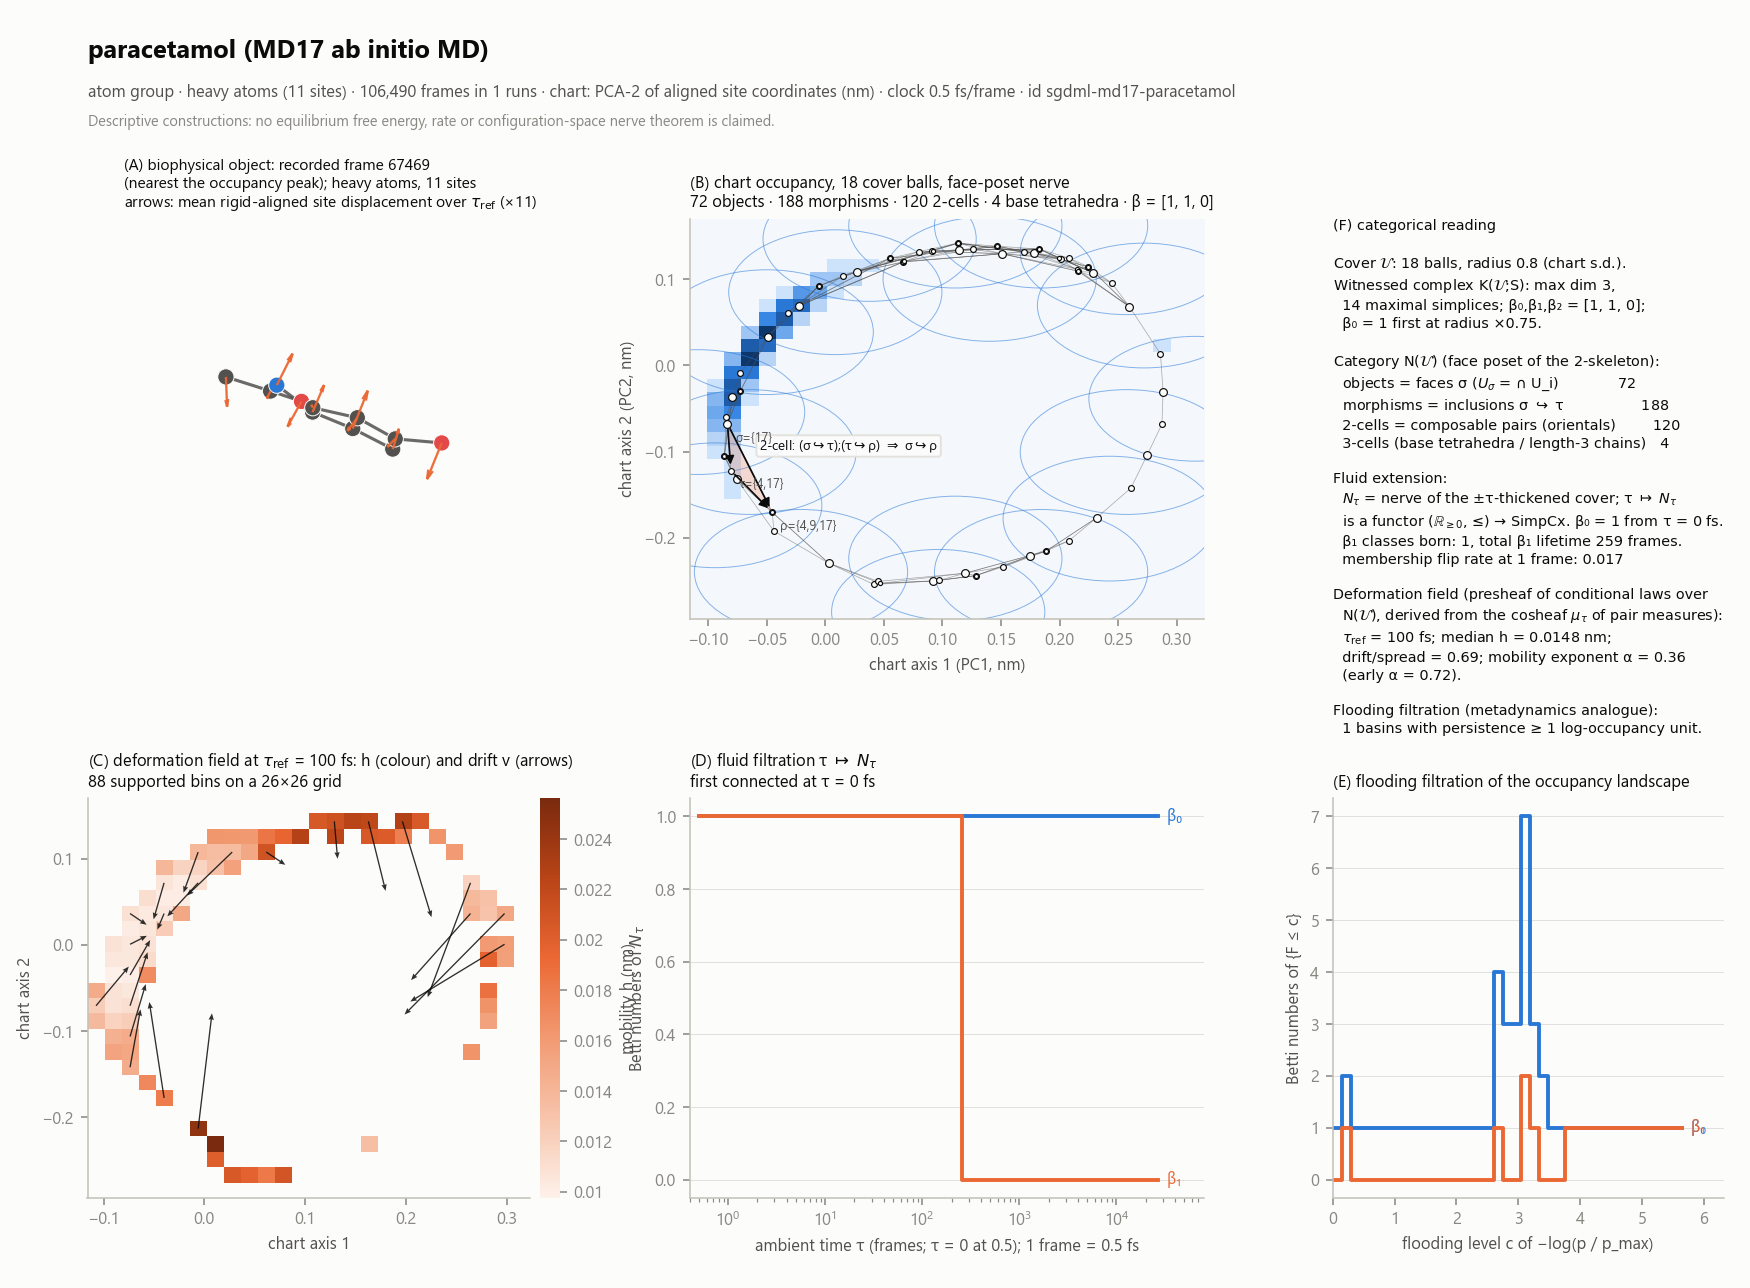
\includegraphics[width=\linewidth,height=.93\textheight,keepaspectratio]{systems/sgdml-md17-paracetamol/plate.png}\caption{paracetamol (MD17 ab initio MD) (\texttt{sgdml-md17-paracetamol}). Source: https://www.quantum-machine.org/gdml/data/npz/paracetamol\_dft.npz.}\end{figure}\clearpage
\begin{figure}[H]\centering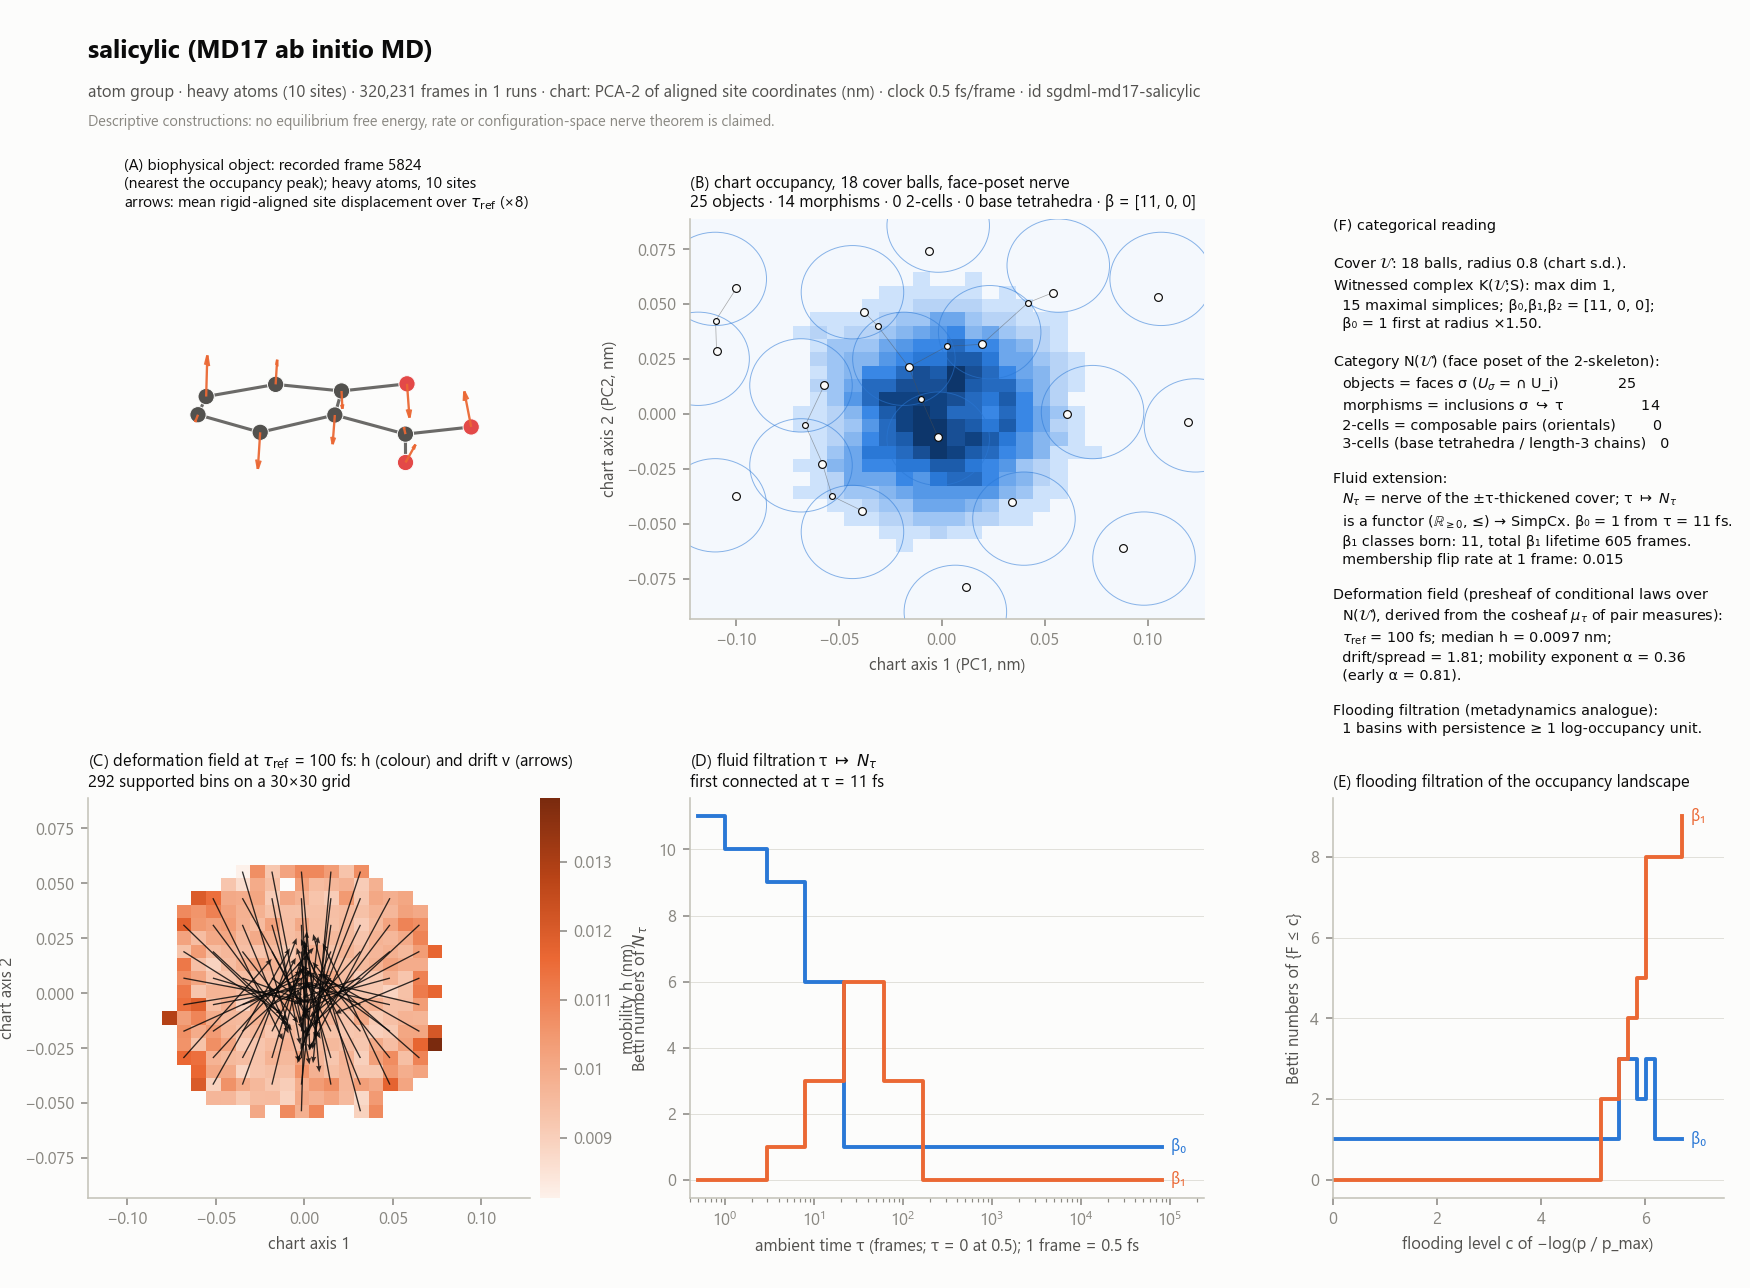
\includegraphics[width=\linewidth,height=.93\textheight,keepaspectratio]{systems/sgdml-md17-salicylic/plate.png}\caption{salicylic (MD17 ab initio MD) (\texttt{sgdml-md17-salicylic}). Source: https://www.quantum-machine.org/gdml/data/npz/md17\_salicylic.npz.}\end{figure}\clearpage
\begin{figure}[H]\centering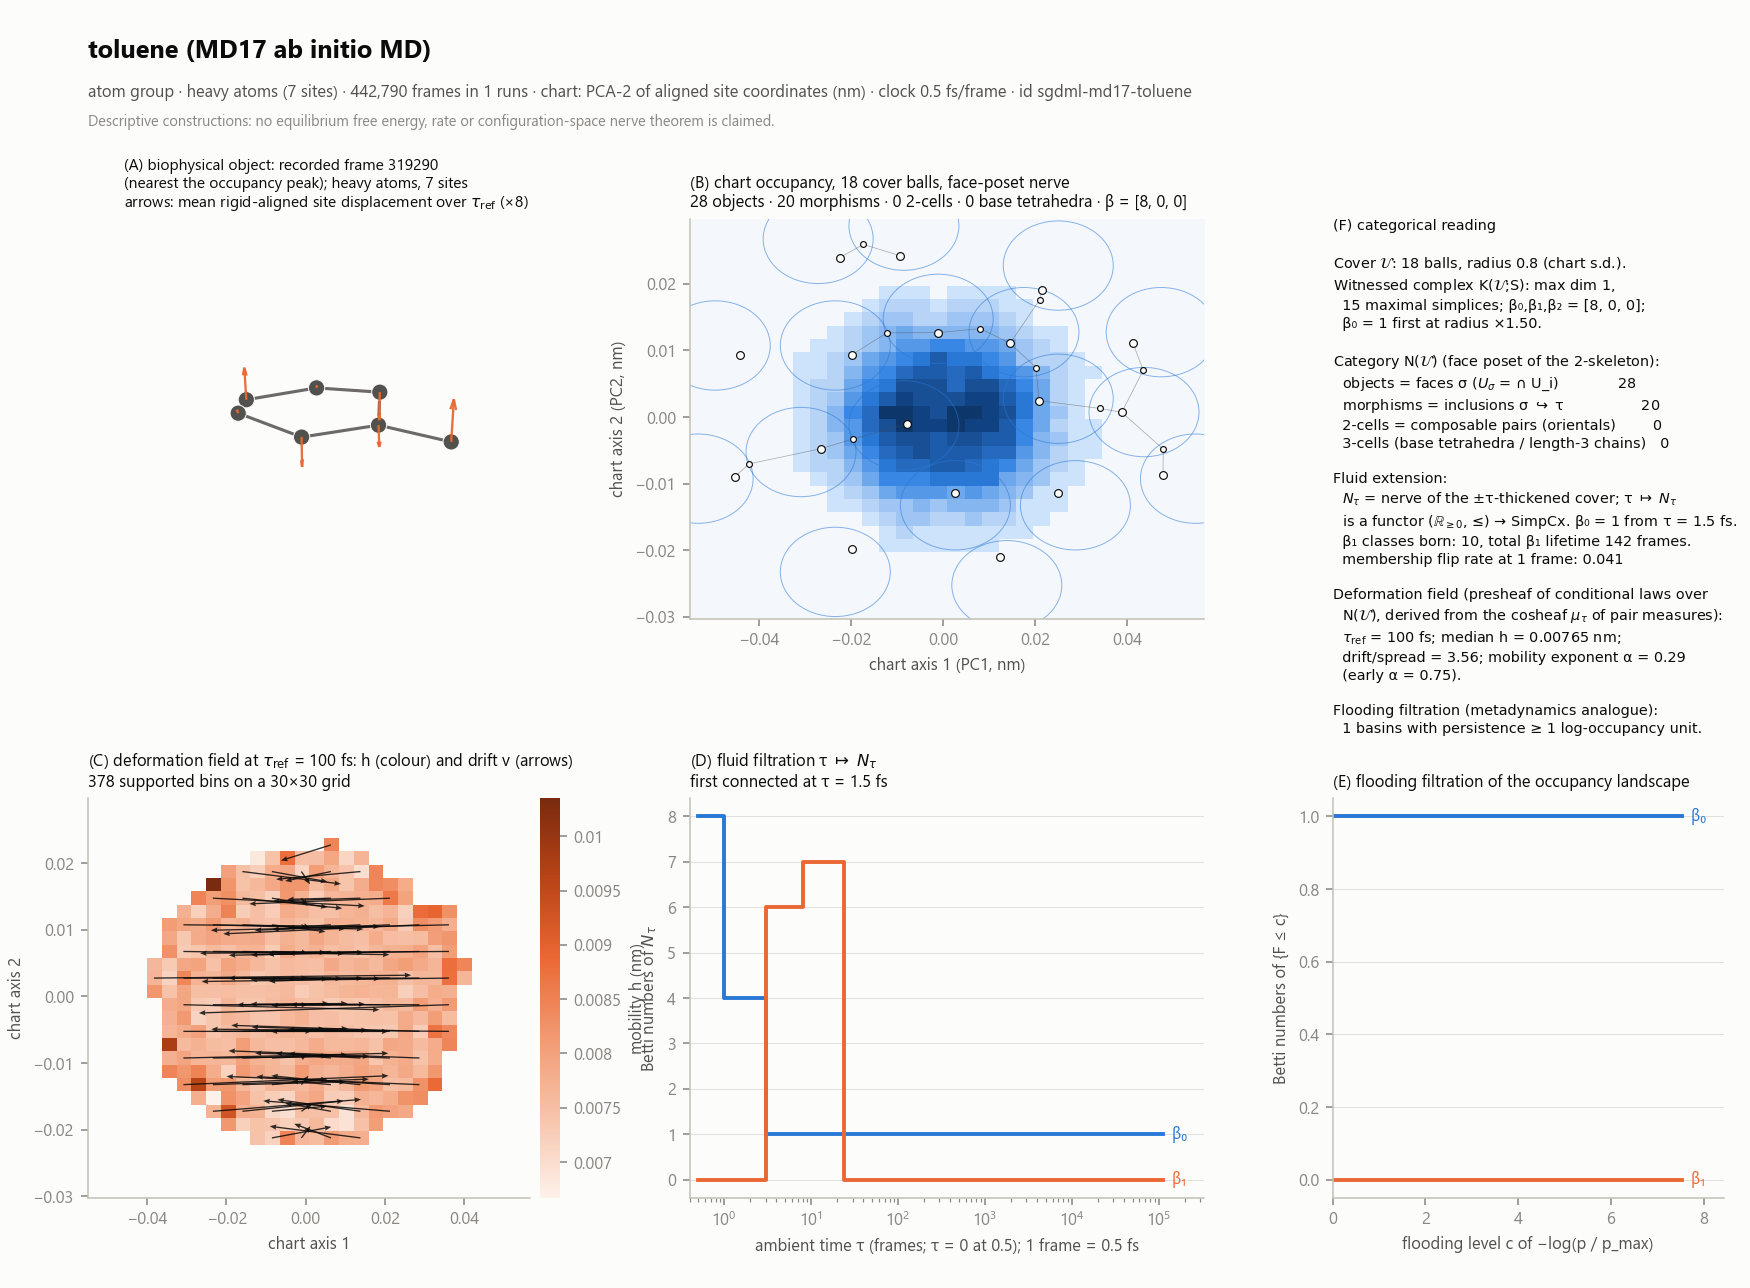
\includegraphics[width=\linewidth,height=.93\textheight,keepaspectratio]{systems/sgdml-md17-toluene/plate.png}\caption{toluene (MD17 ab initio MD) (\texttt{sgdml-md17-toluene}). Source: https://www.quantum-machine.org/gdml/data/npz/md17\_toluene.npz.}\end{figure}\clearpage
\begin{figure}[H]\centering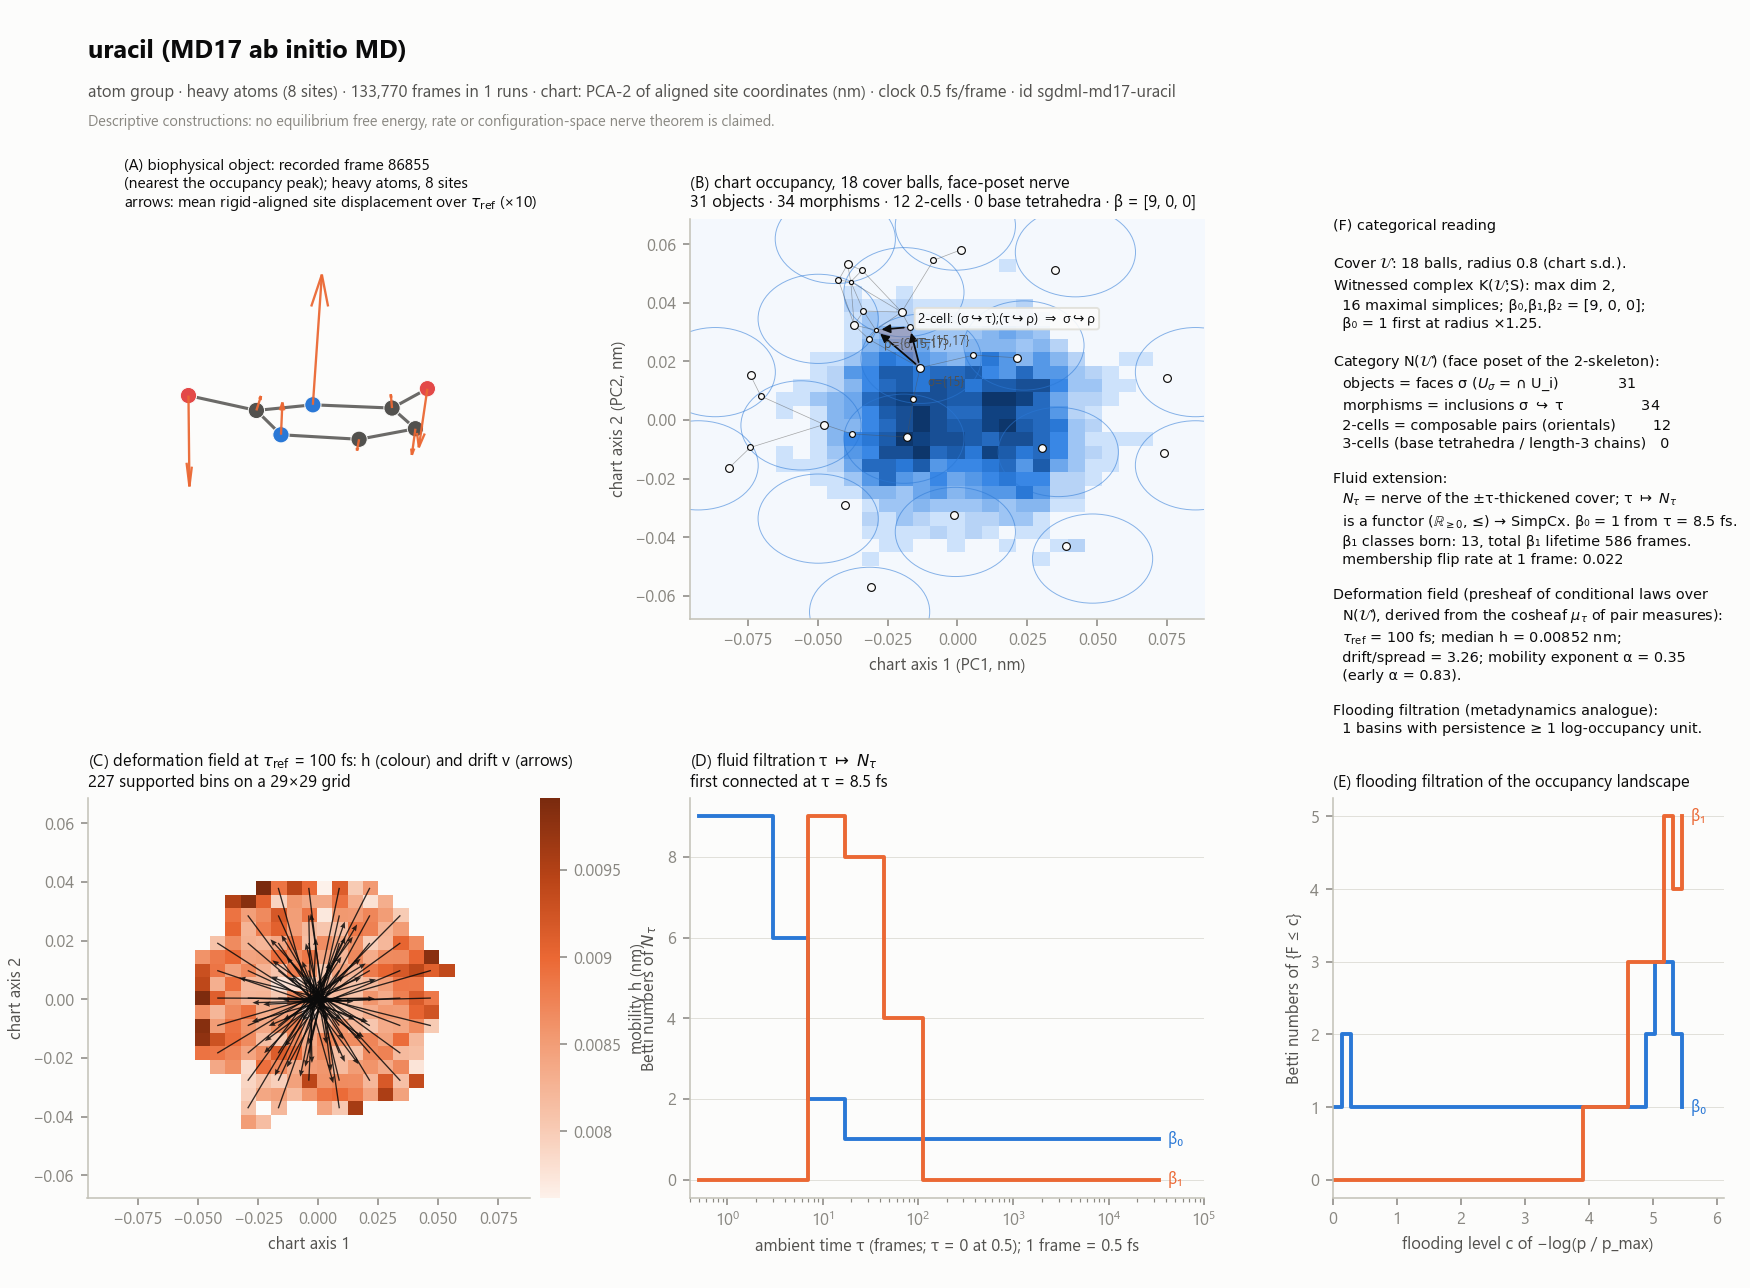
\includegraphics[width=\linewidth,height=.93\textheight,keepaspectratio]{systems/sgdml-md17-uracil/plate.png}\caption{uracil (MD17 ab initio MD) (\texttt{sgdml-md17-uracil}). Source: https://www.quantum-machine.org/gdml/data/npz/md17\_uracil.npz.}\end{figure}\clearpage
\begin{figure}[H]\centering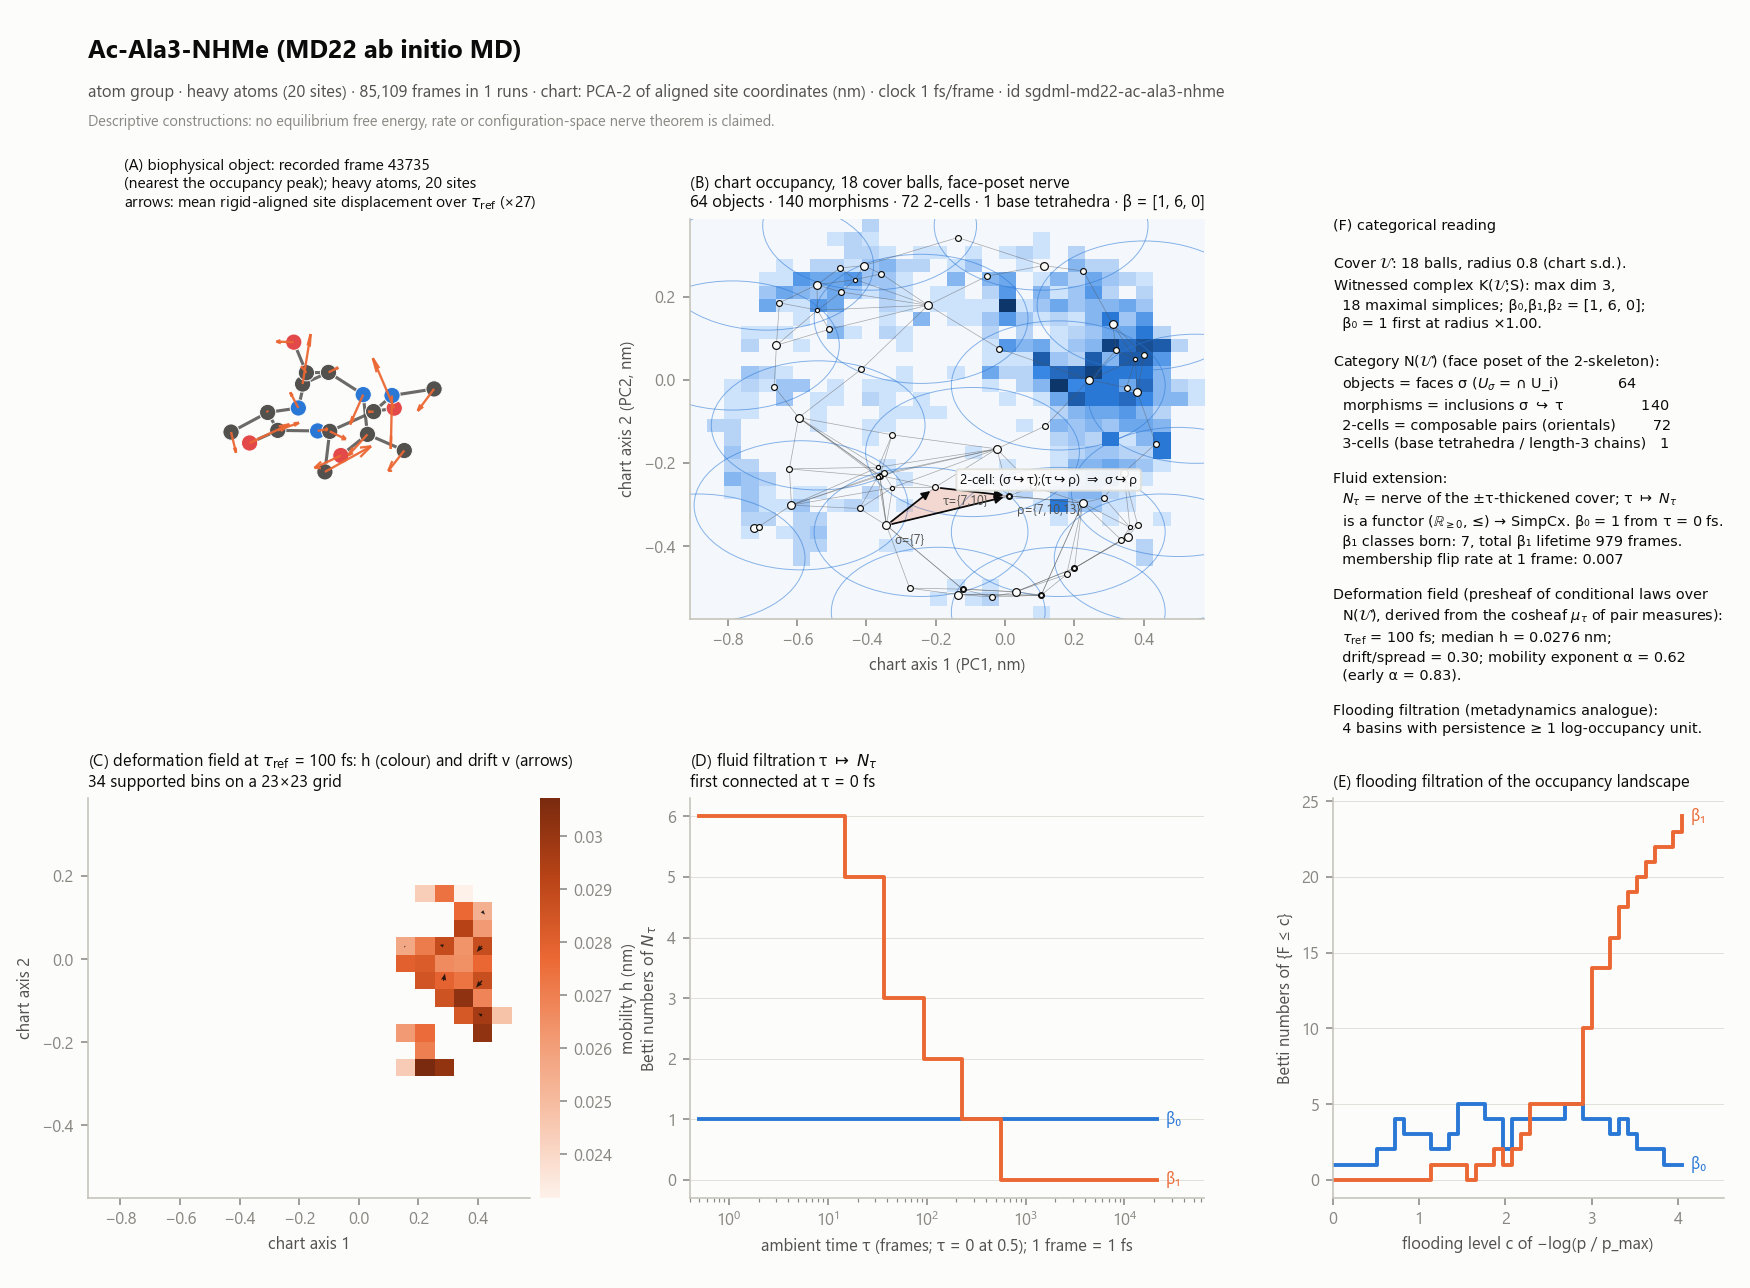
\includegraphics[width=\linewidth,height=.93\textheight,keepaspectratio]{systems/sgdml-md22-ac-ala3-nhme/plate.png}\caption{Ac-Ala3-NHMe (MD22 ab initio MD) (\texttt{sgdml-md22-ac-ala3-nhme}). Source: https://www.quantum-machine.org/gdml/data/npz/md22\_Ac-Ala3-NHMe.npz.}\end{figure}\clearpage
\begin{figure}[H]\centering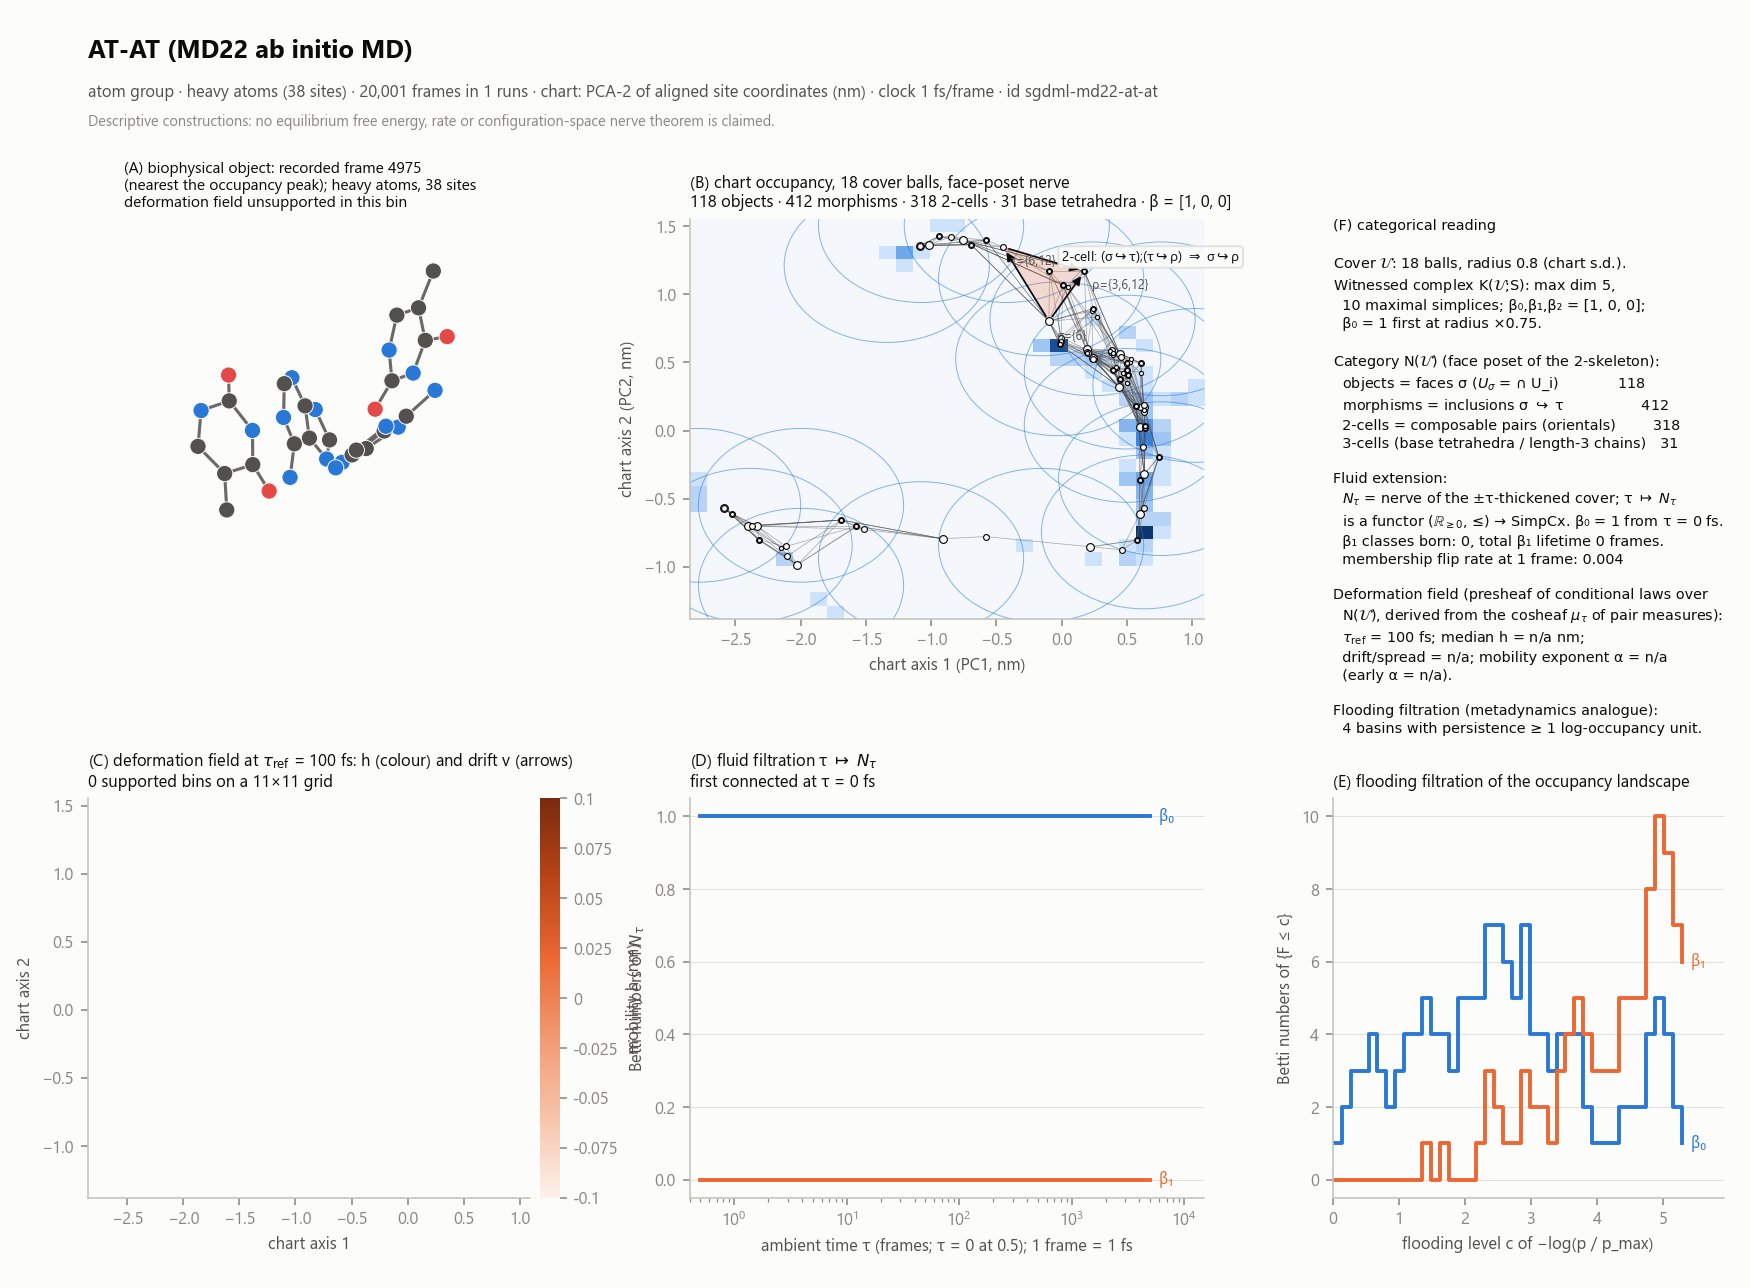
\includegraphics[width=\linewidth,height=.93\textheight,keepaspectratio]{systems/sgdml-md22-at-at/plate.png}\caption{AT-AT (MD22 ab initio MD) (\texttt{sgdml-md22-at-at}). Source: https://www.quantum-machine.org/gdml/data/npz/md22\_AT-AT.npz.}\end{figure}\clearpage
\begin{figure}[H]\centering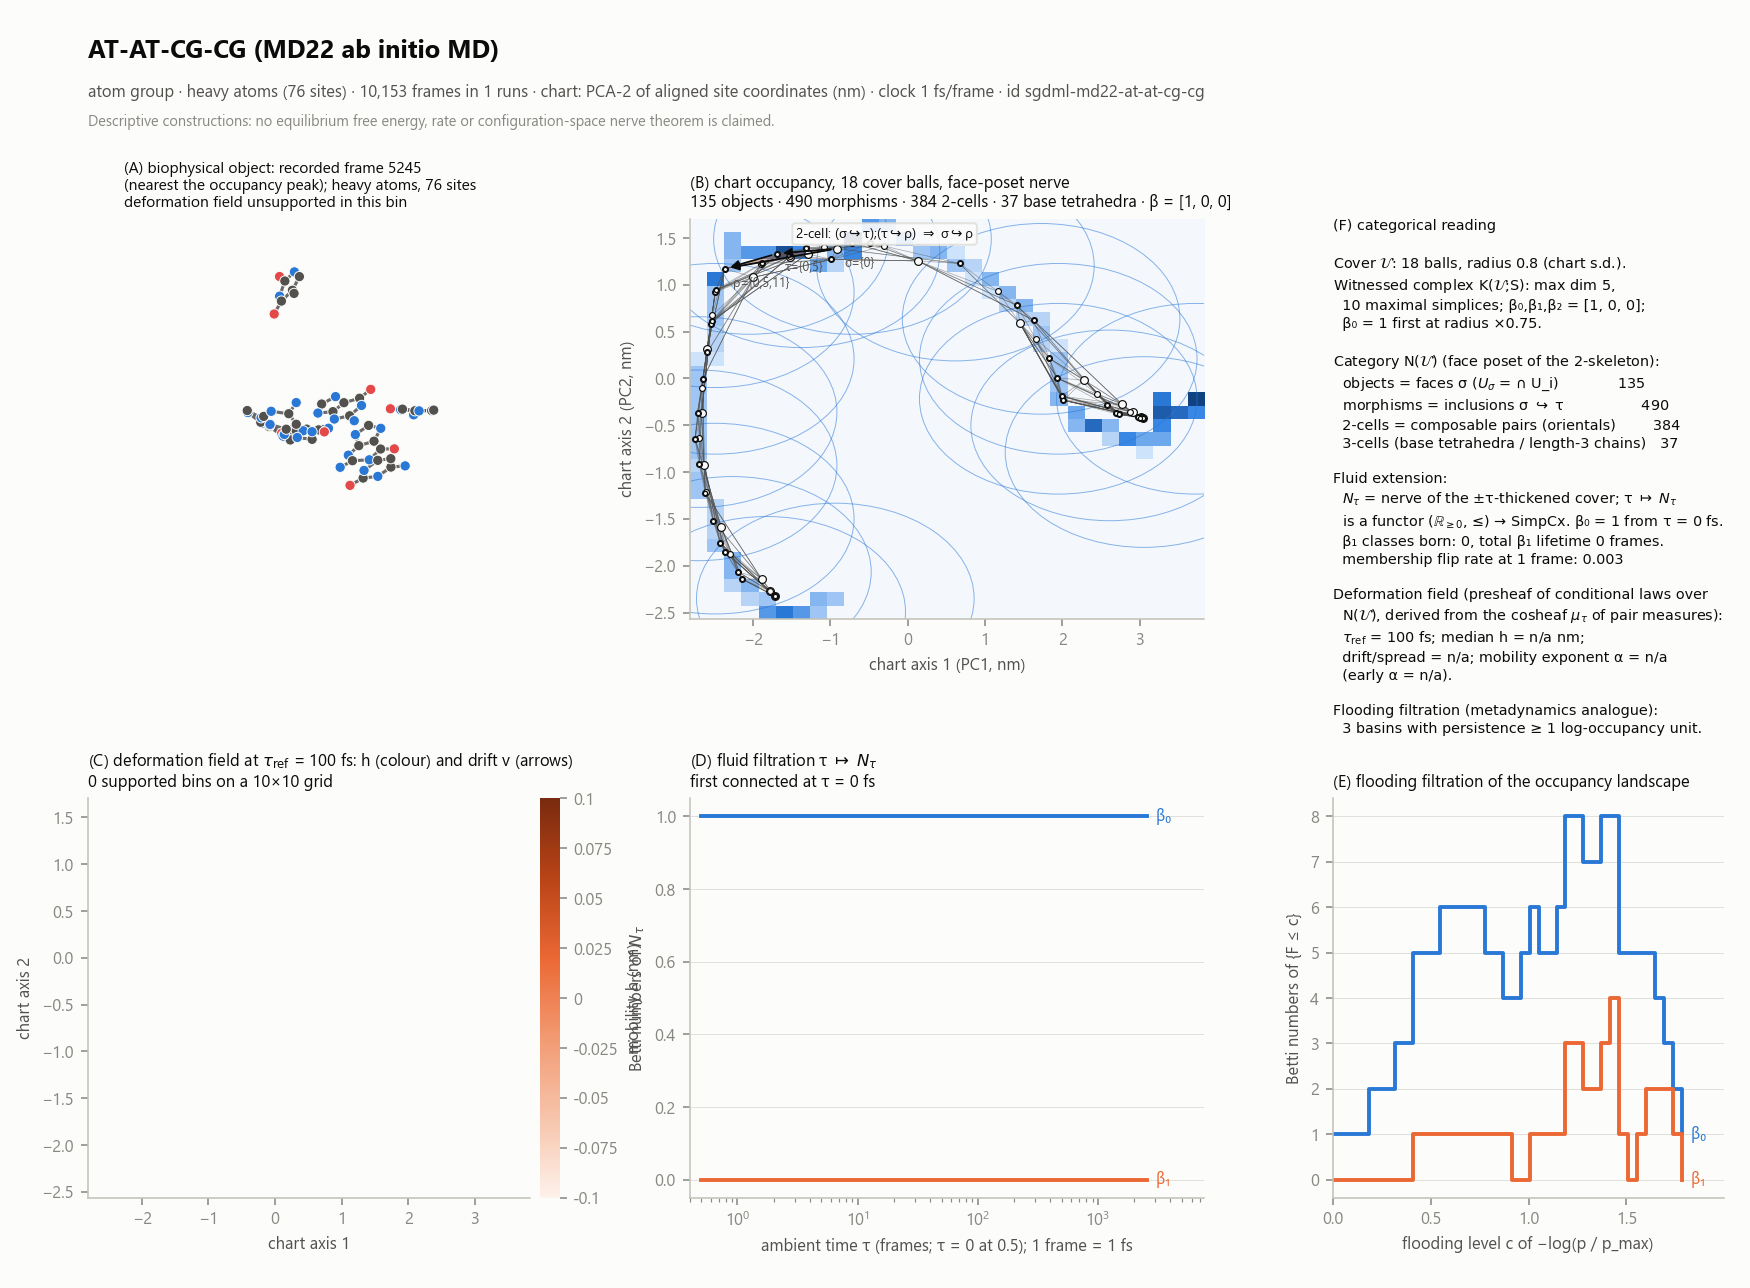
\includegraphics[width=\linewidth,height=.93\textheight,keepaspectratio]{systems/sgdml-md22-at-at-cg-cg/plate.png}\caption{AT-AT-CG-CG (MD22 ab initio MD) (\texttt{sgdml-md22-at-at-cg-cg}). Source: https://www.quantum-machine.org/gdml/data/npz/md22\_AT-AT-CG-CG.npz.}\end{figure}\clearpage
\begin{figure}[H]\centering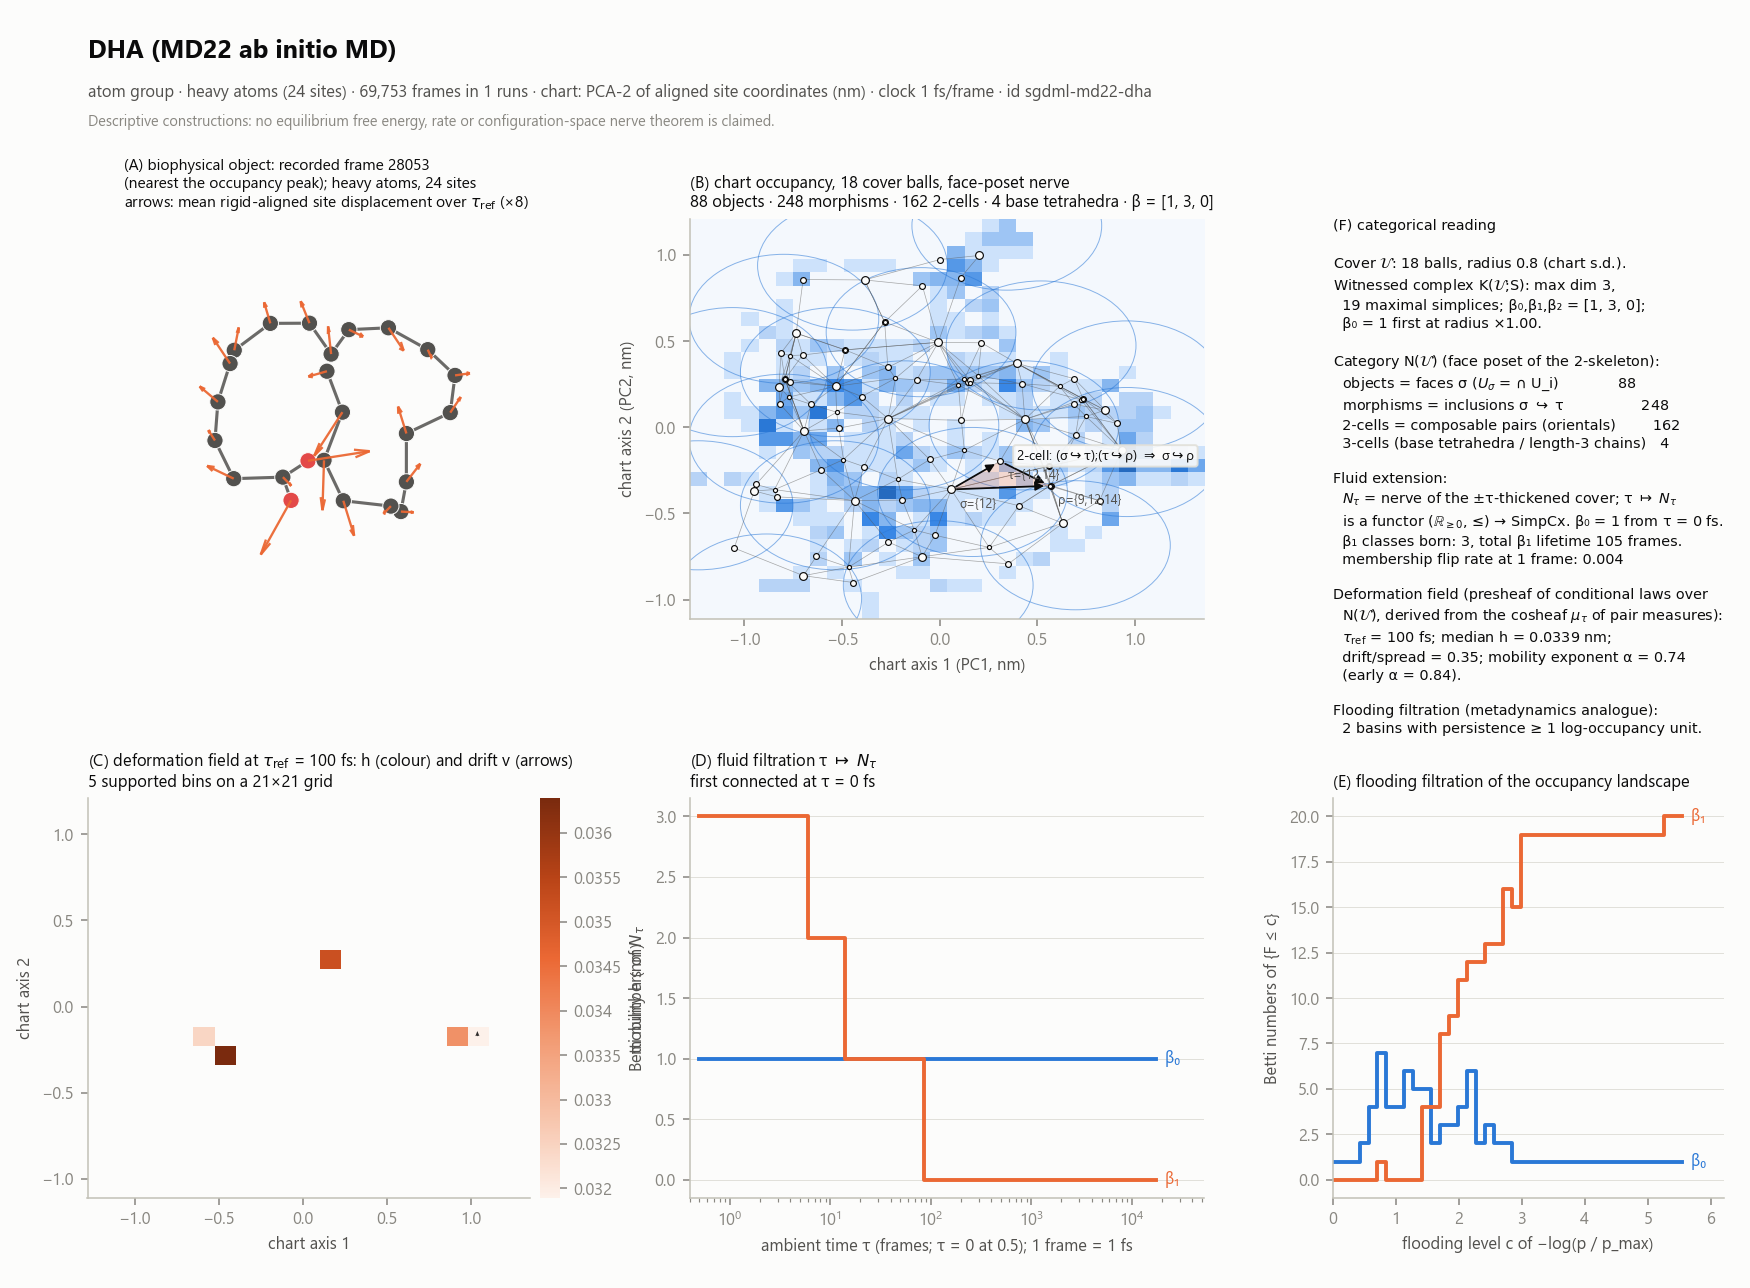
\includegraphics[width=\linewidth,height=.93\textheight,keepaspectratio]{systems/sgdml-md22-dha/plate.png}\caption{DHA (MD22 ab initio MD) (\texttt{sgdml-md22-dha}). Source: https://www.quantum-machine.org/gdml/data/npz/md22\_DHA.npz.}\end{figure}\clearpage
\begin{figure}[H]\centering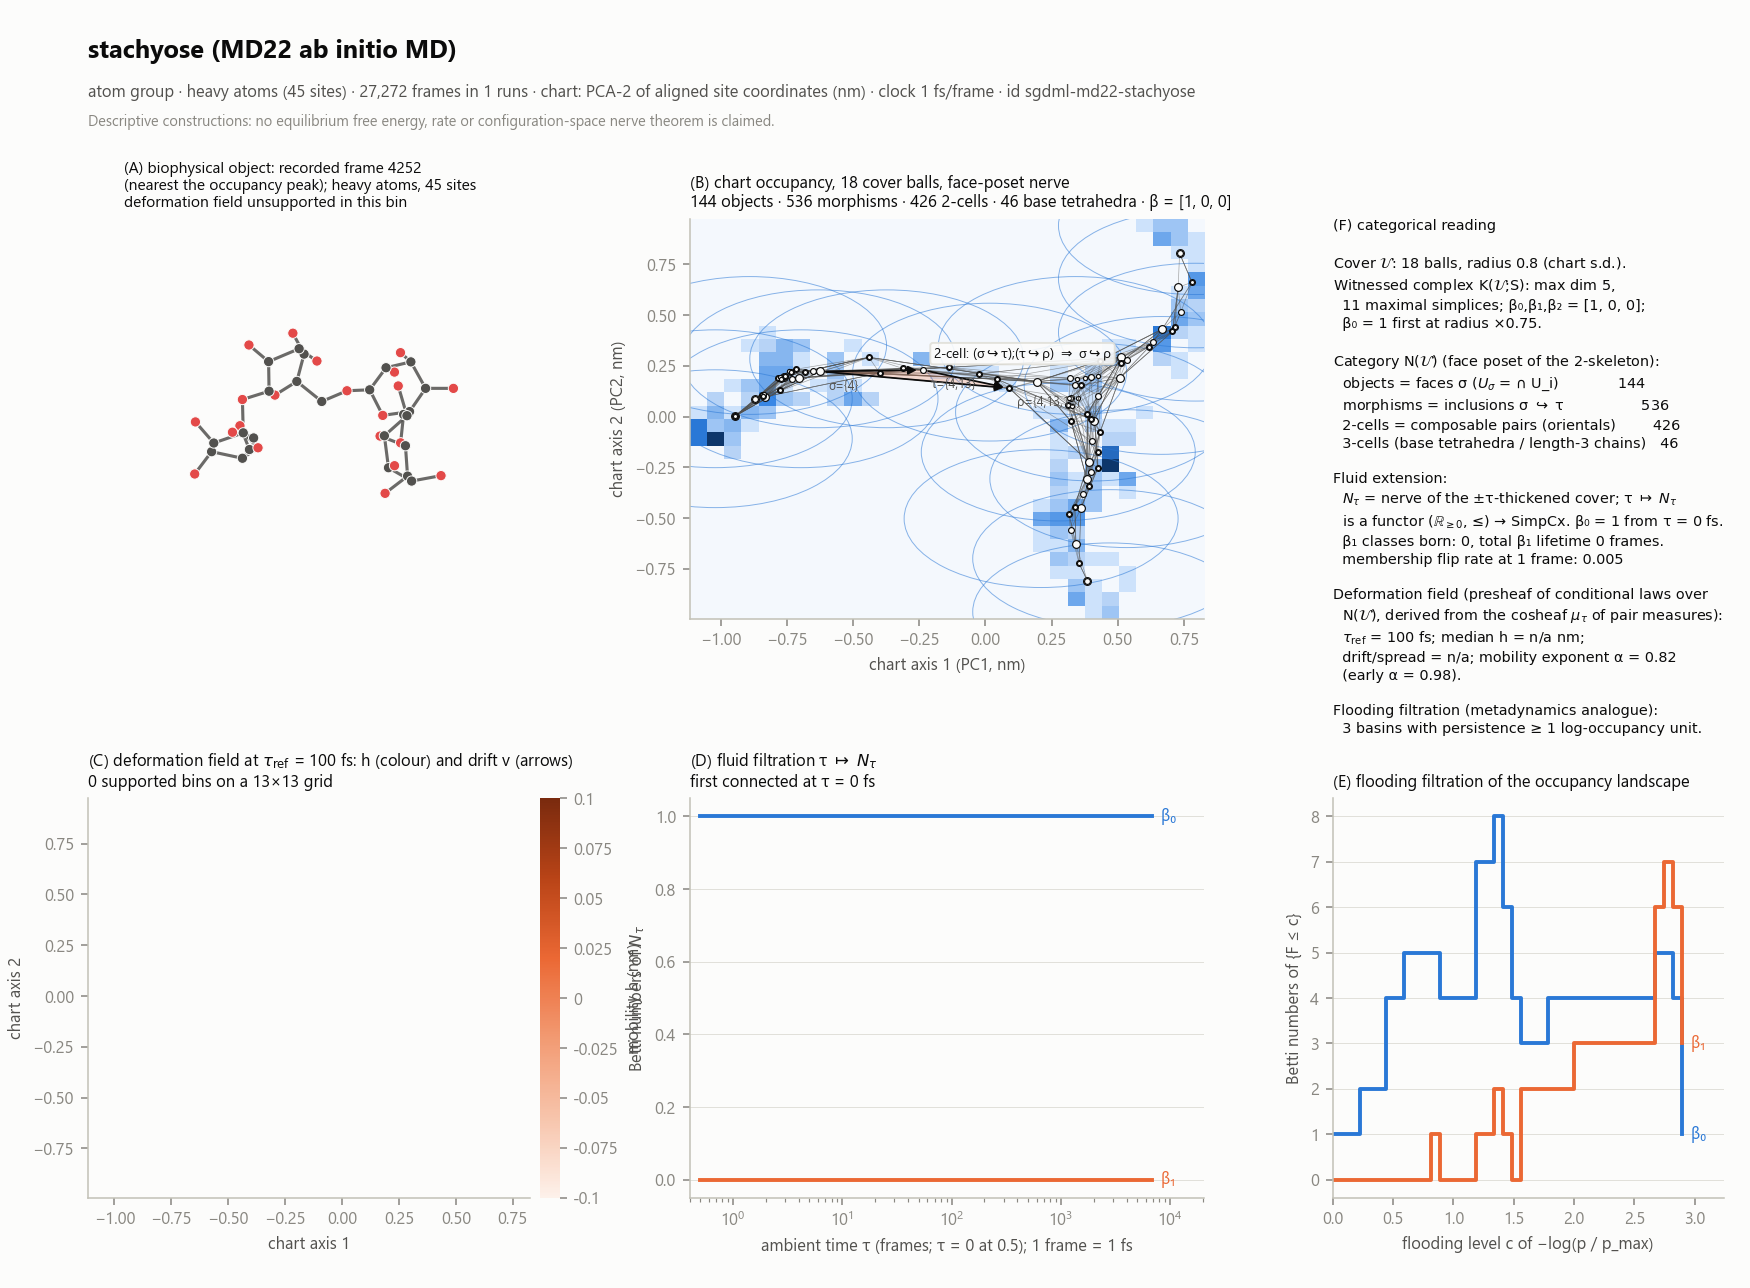
\includegraphics[width=\linewidth,height=.93\textheight,keepaspectratio]{systems/sgdml-md22-stachyose/plate.png}\caption{stachyose (MD22 ab initio MD) (\texttt{sgdml-md22-stachyose}). Source: https://www.quantum-machine.org/gdml/data/npz/md22\_stachyose.npz.}\end{figure}\clearpage
\begin{figure}[H]\centering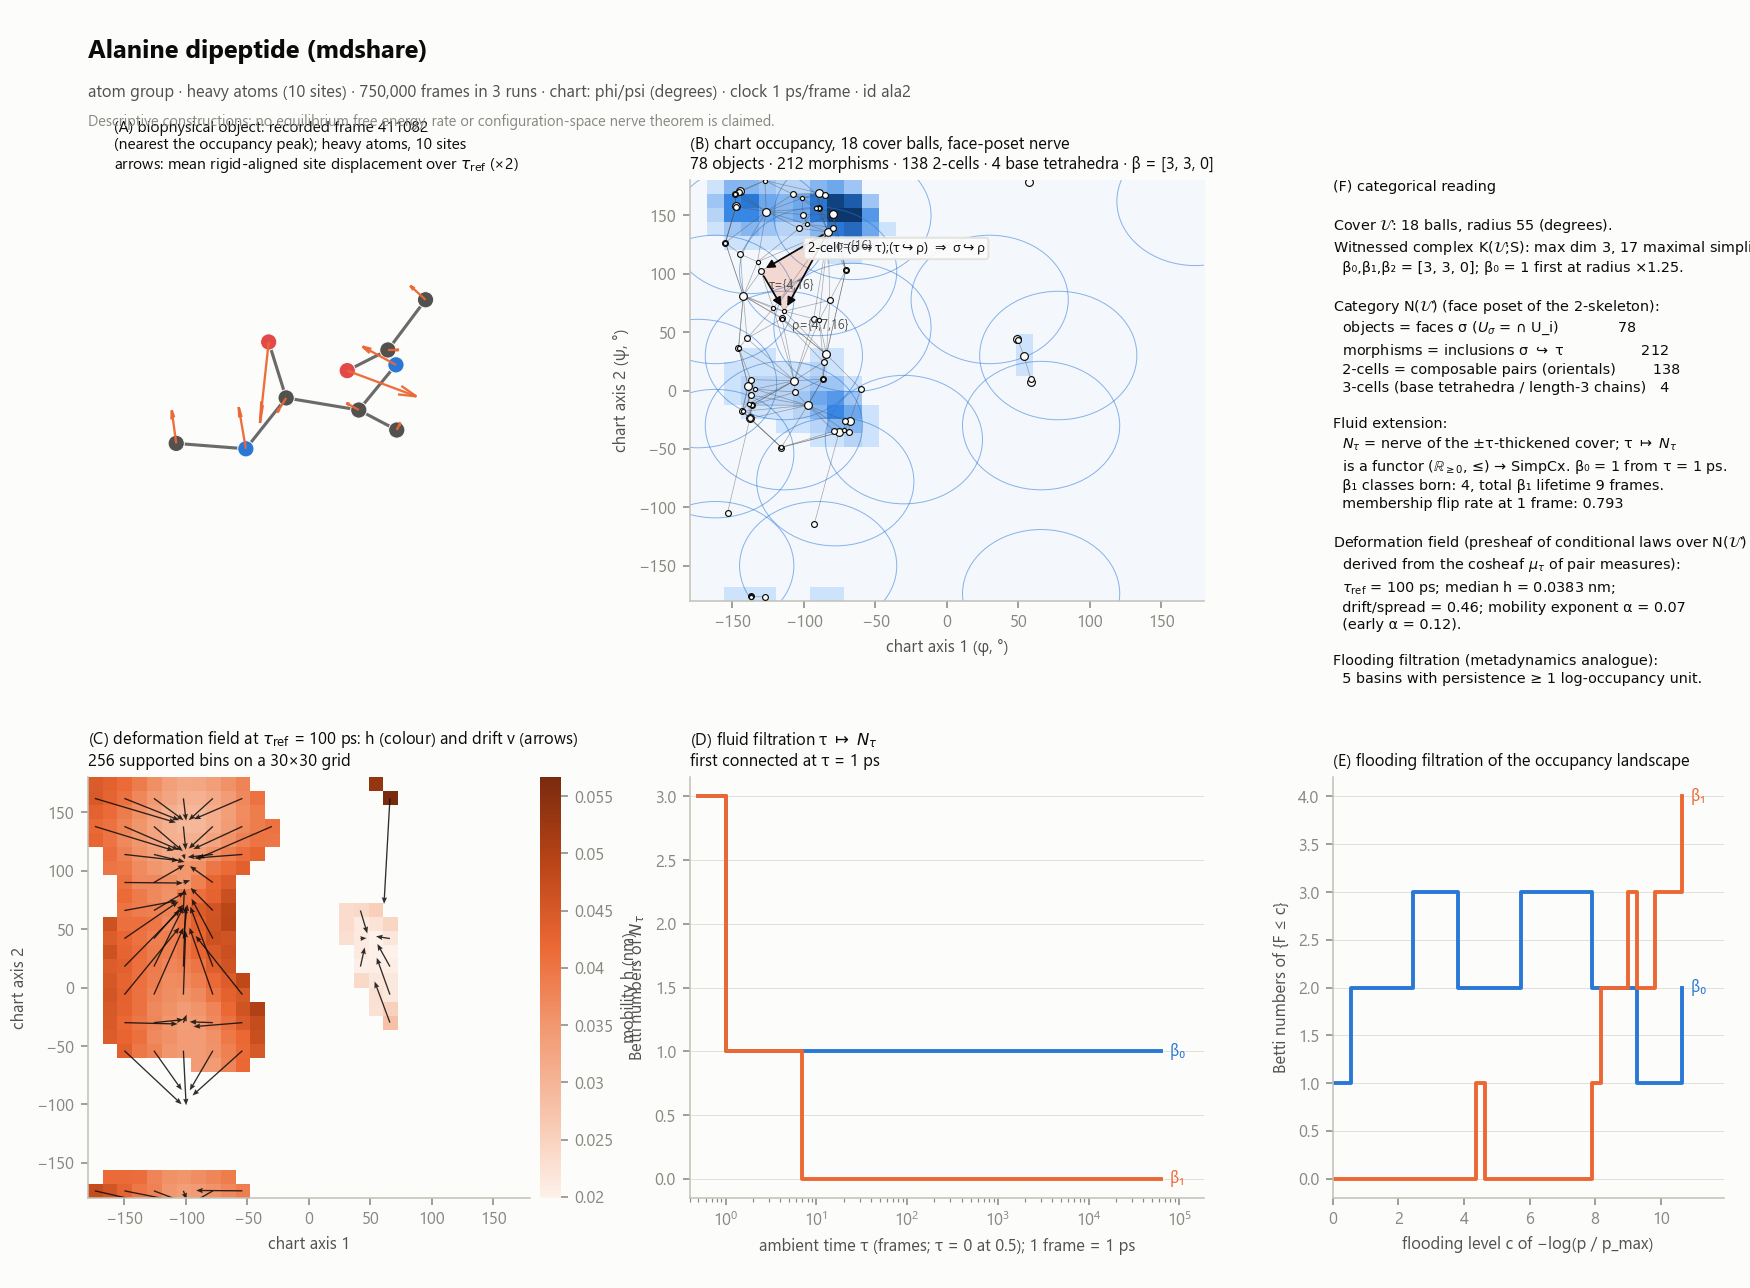
\includegraphics[width=\linewidth,height=.93\textheight,keepaspectratio]{systems/ala2/plate.png}\caption{Alanine dipeptide (mdshare) (\texttt{ala2}). Source: https://markovmodel.github.io/mdshare/ALA2/.}\end{figure}\clearpage
\begin{figure}[H]\centering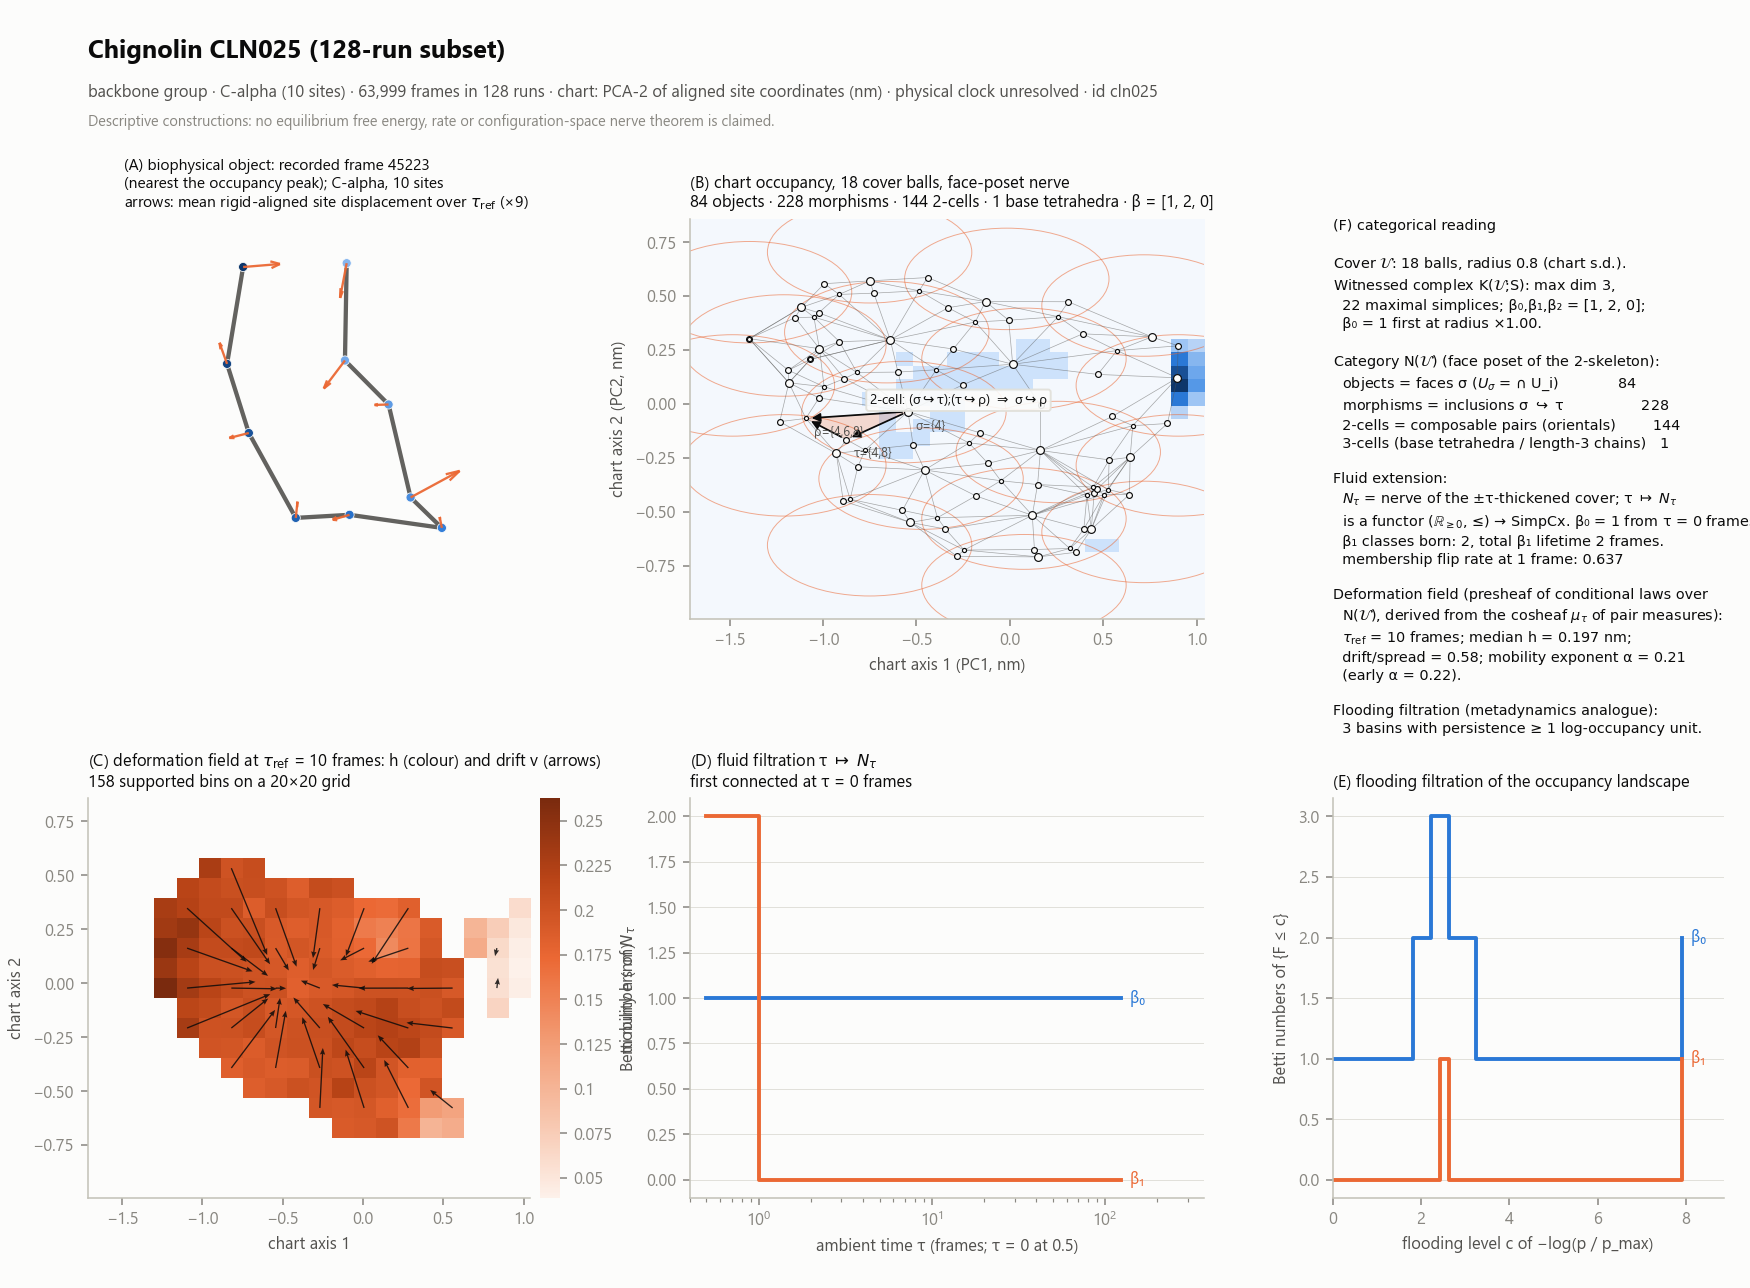
\includegraphics[width=\linewidth,height=.93\textheight,keepaspectratio]{systems/cln025/plate.png}\caption{Chignolin CLN025 (128-run subset) (\texttt{cln025}). Source: https://ndownloader.figshare.com/files/26424614.}\end{figure}\clearpage
\begin{figure}[H]\centering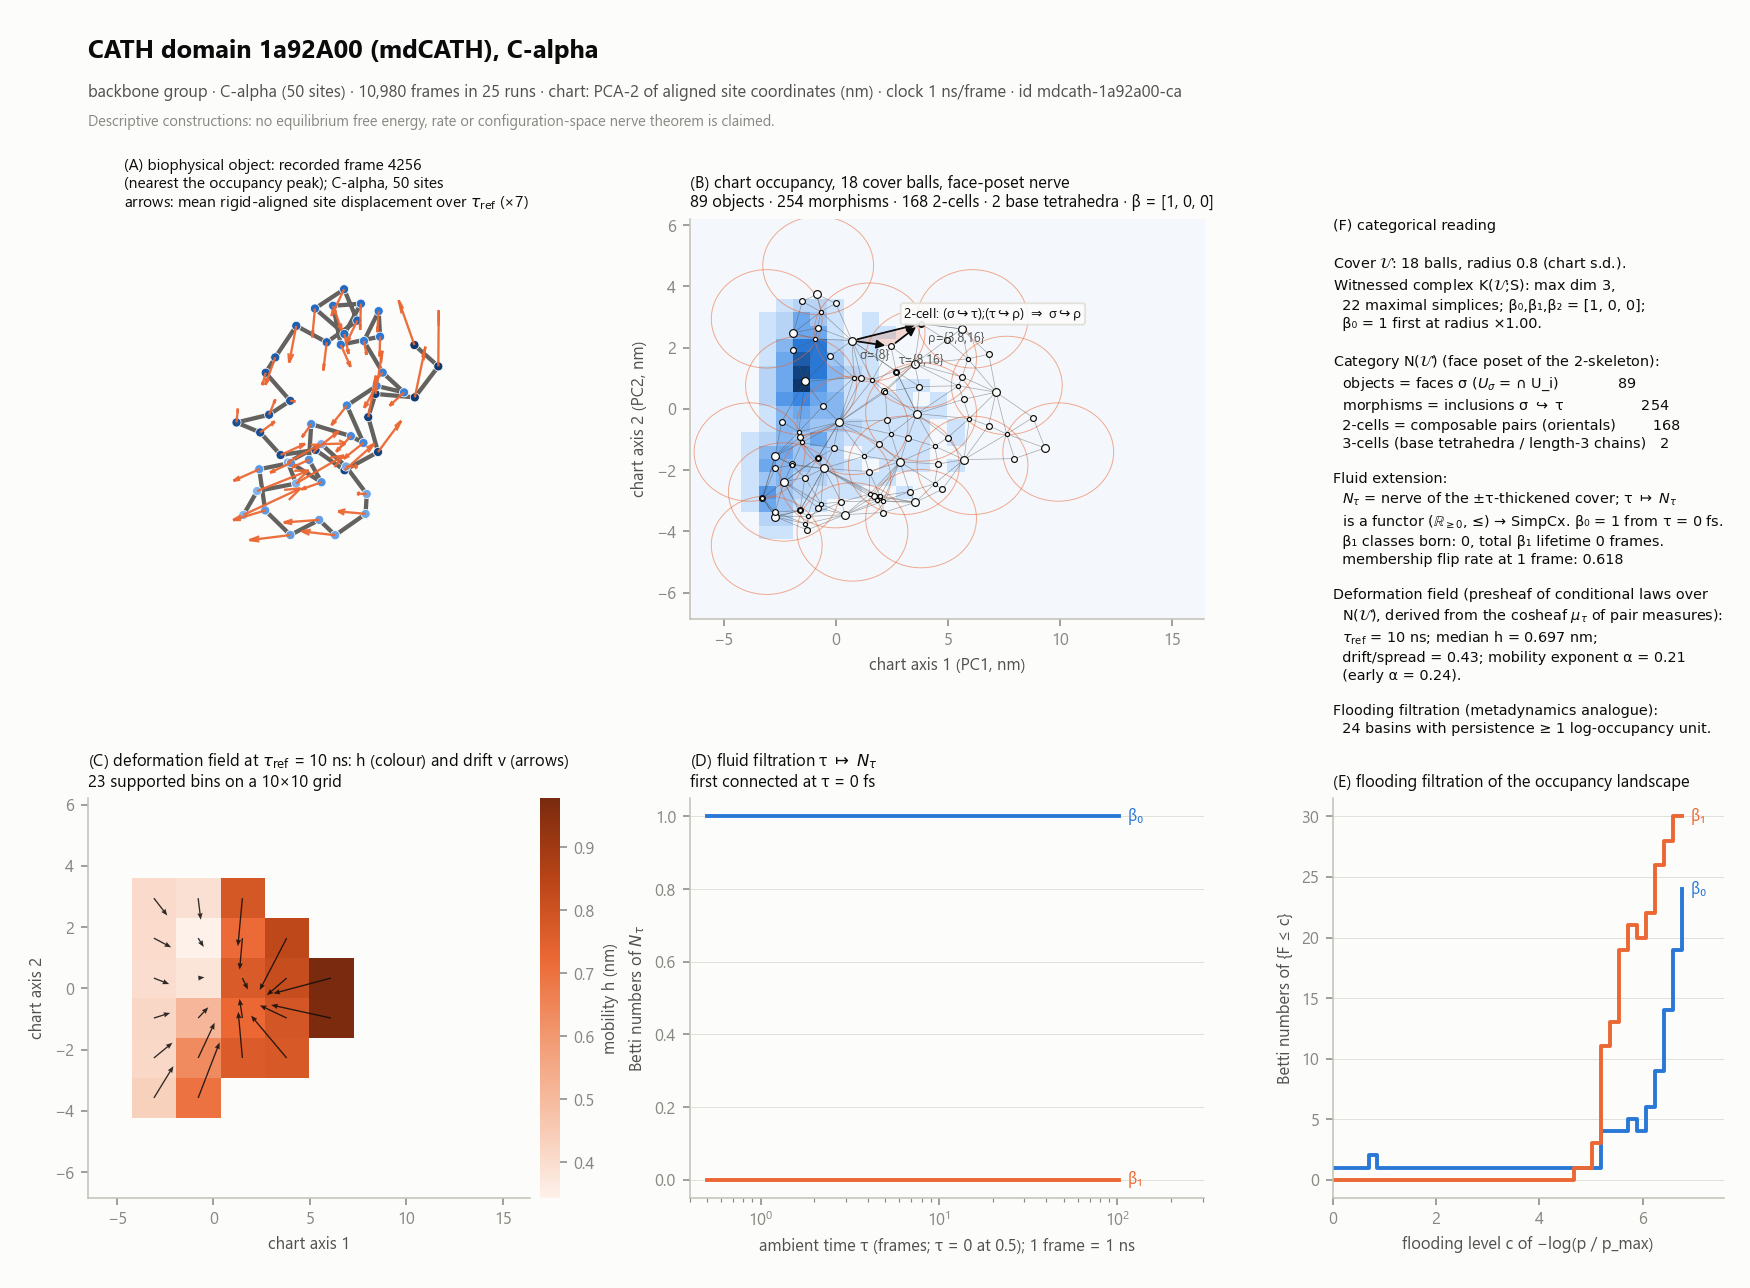
\includegraphics[width=\linewidth,height=.93\textheight,keepaspectratio]{systems/mdcath-1a92a00-ca/plate.png}\caption{CATH domain 1a92A00 (mdCATH), C-alpha (\texttt{mdcath-1a92a00-ca}). Source: https://huggingface.co/datasets/compsciencelab/mdCATH/resolve/main/data/mdcath\_dataset\_1a92A00.h5.}\end{figure}\clearpage
\begin{figure}[H]\centering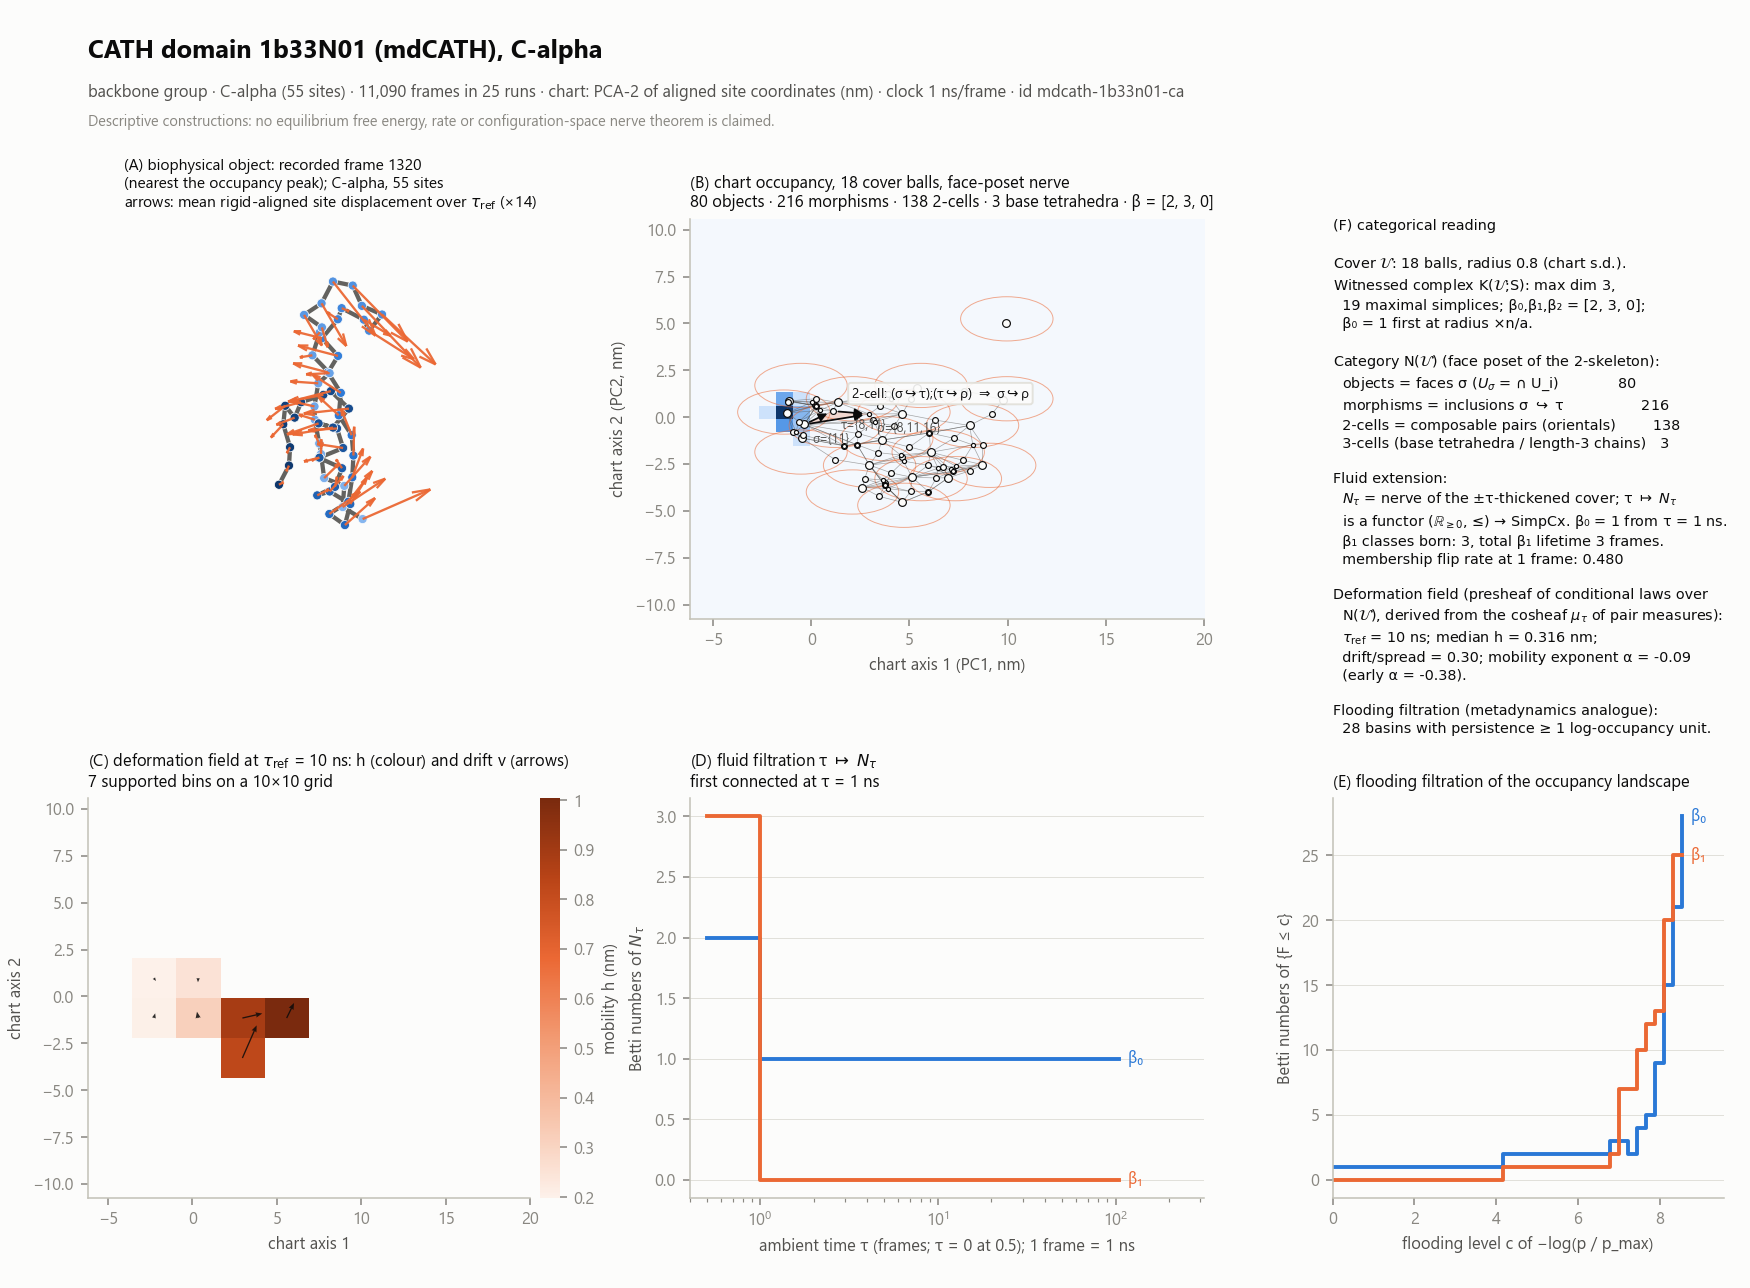
\includegraphics[width=\linewidth,height=.93\textheight,keepaspectratio]{systems/mdcath-1b33n01-ca/plate.png}\caption{CATH domain 1b33N01 (mdCATH), C-alpha (\texttt{mdcath-1b33n01-ca}). Source: https://huggingface.co/datasets/compsciencelab/mdCATH/resolve/main/data/mdcath\_dataset\_1b33N01.h5.}\end{figure}\clearpage
\begin{figure}[H]\centering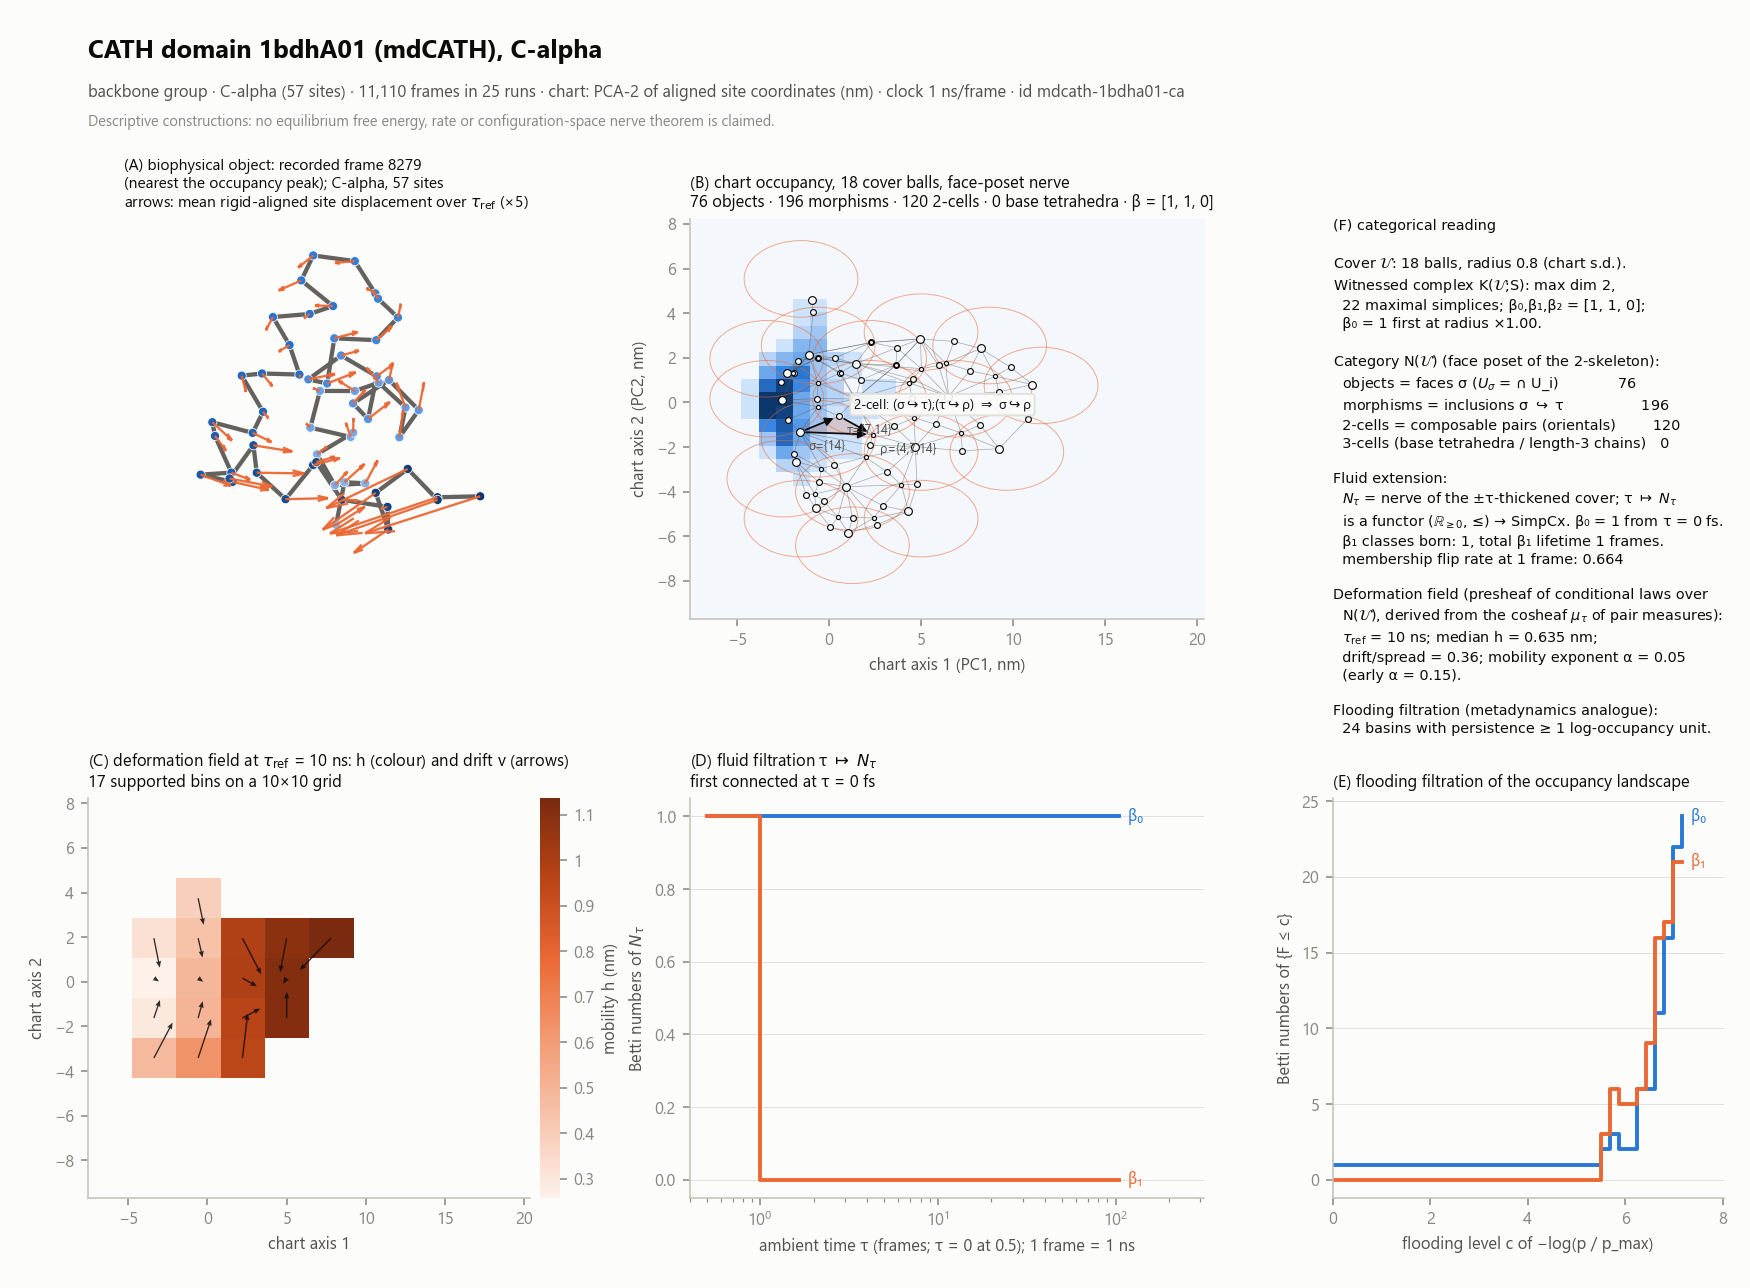
\includegraphics[width=\linewidth,height=.93\textheight,keepaspectratio]{systems/mdcath-1bdha01-ca/plate.png}\caption{CATH domain 1bdhA01 (mdCATH), C-alpha (\texttt{mdcath-1bdha01-ca}). Source: https://huggingface.co/datasets/compsciencelab/mdCATH/resolve/main/data/mdcath\_dataset\_1bdhA01.h5.}\end{figure}\clearpage
\begin{figure}[H]\centering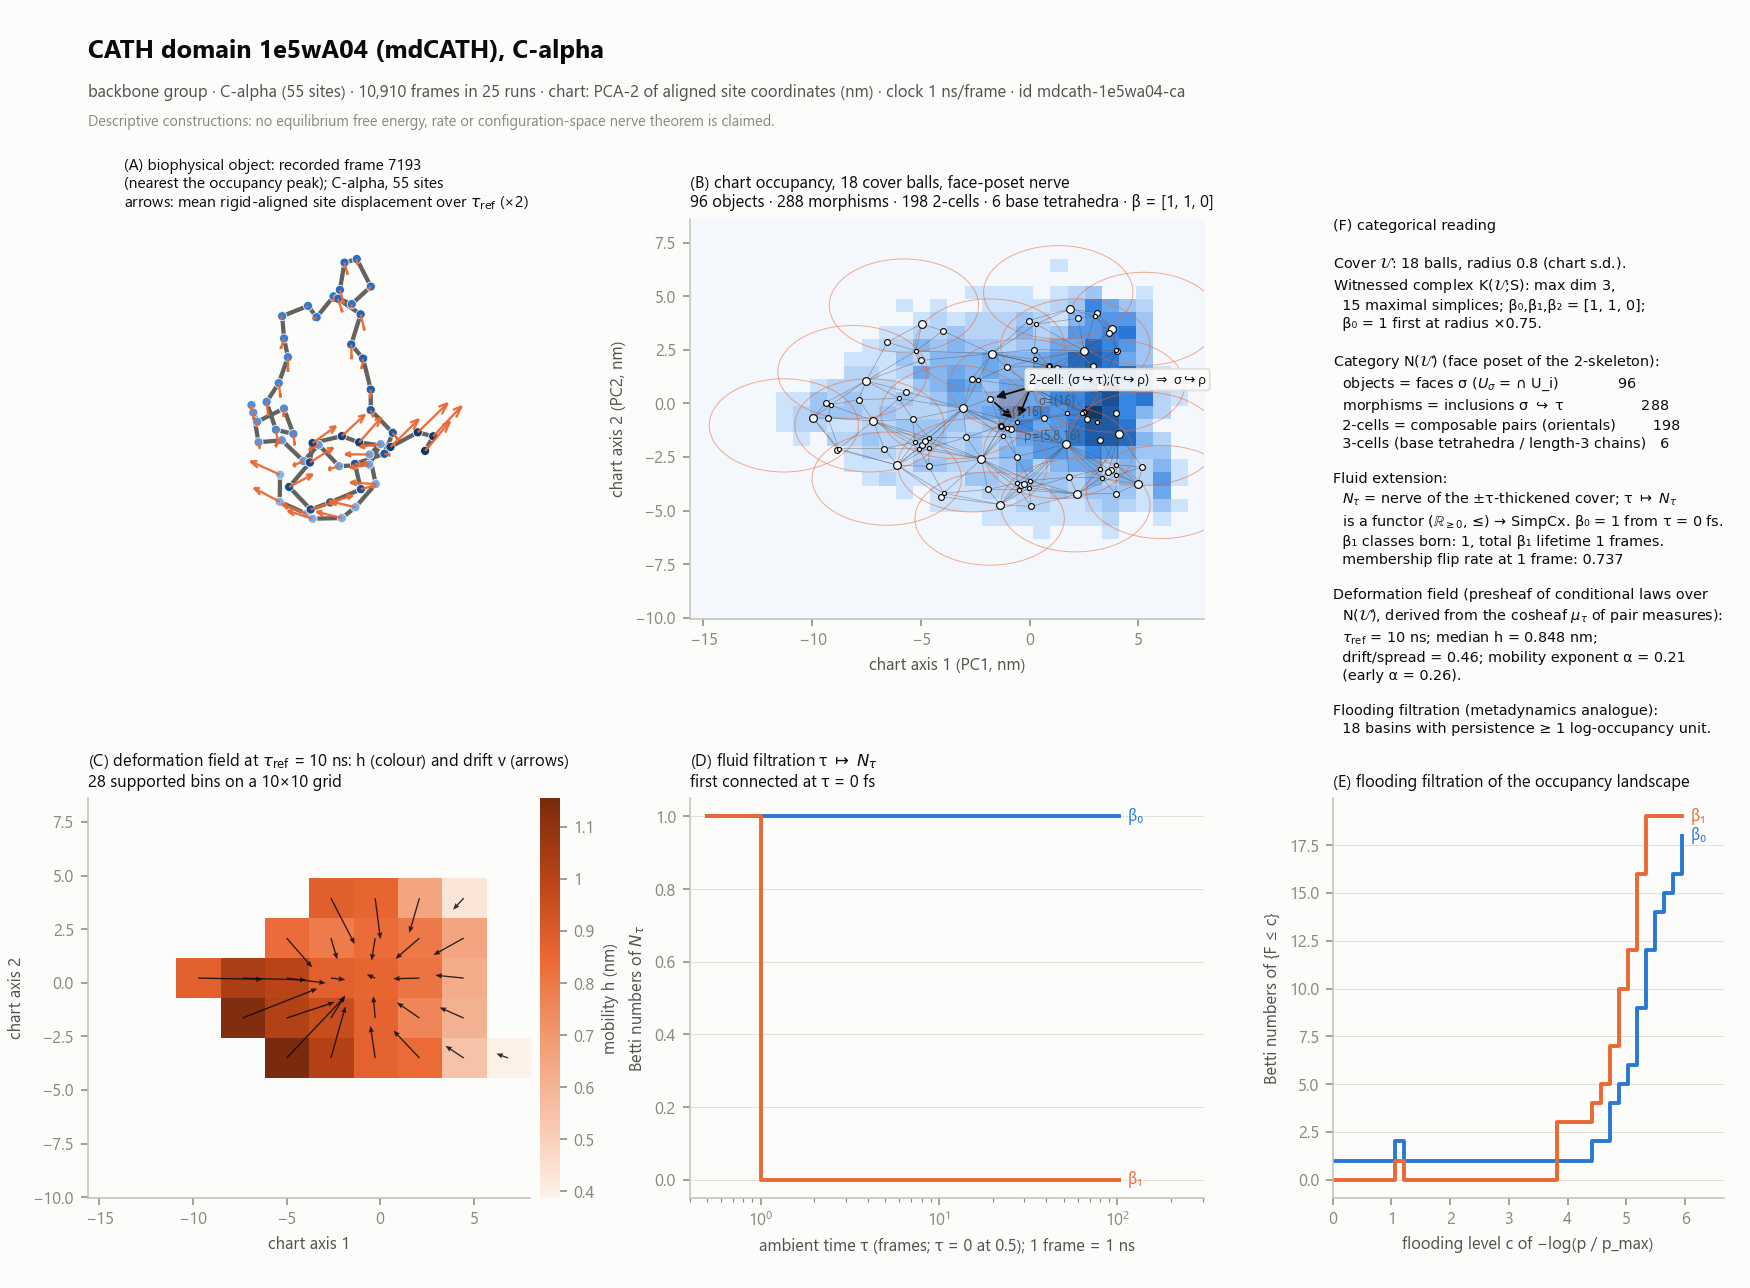
\includegraphics[width=\linewidth,height=.93\textheight,keepaspectratio]{systems/mdcath-1e5wa04-ca/plate.png}\caption{CATH domain 1e5wA04 (mdCATH), C-alpha (\texttt{mdcath-1e5wa04-ca}). Source: https://huggingface.co/datasets/compsciencelab/mdCATH/resolve/main/data/mdcath\_dataset\_1e5wA04.h5.}\end{figure}\clearpage
\begin{figure}[H]\centering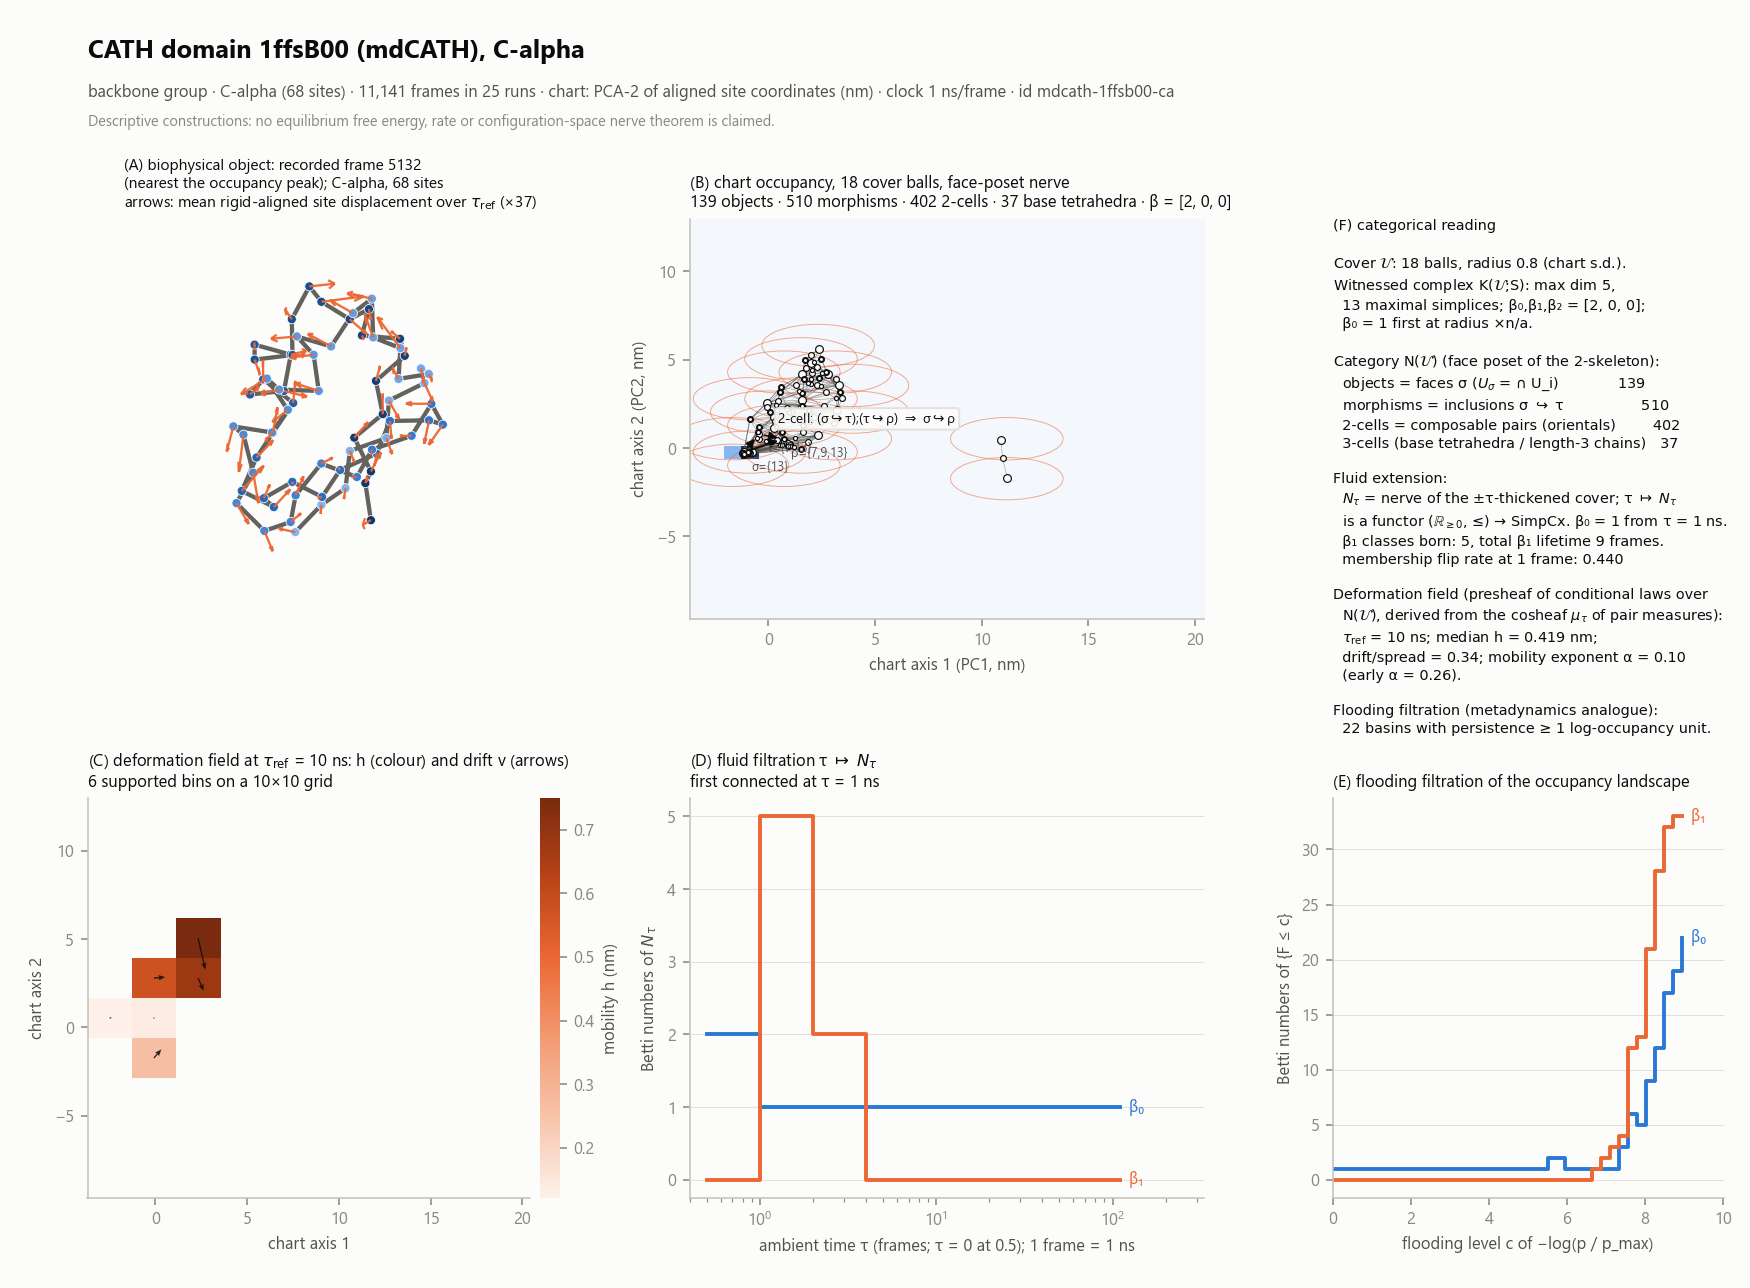
\includegraphics[width=\linewidth,height=.93\textheight,keepaspectratio]{systems/mdcath-1ffsb00-ca/plate.png}\caption{CATH domain 1ffsB00 (mdCATH), C-alpha (\texttt{mdcath-1ffsb00-ca}). Source: https://huggingface.co/datasets/compsciencelab/mdCATH/resolve/main/data/mdcath\_dataset\_1ffsB00.h5.}\end{figure}\clearpage
\begin{figure}[H]\centering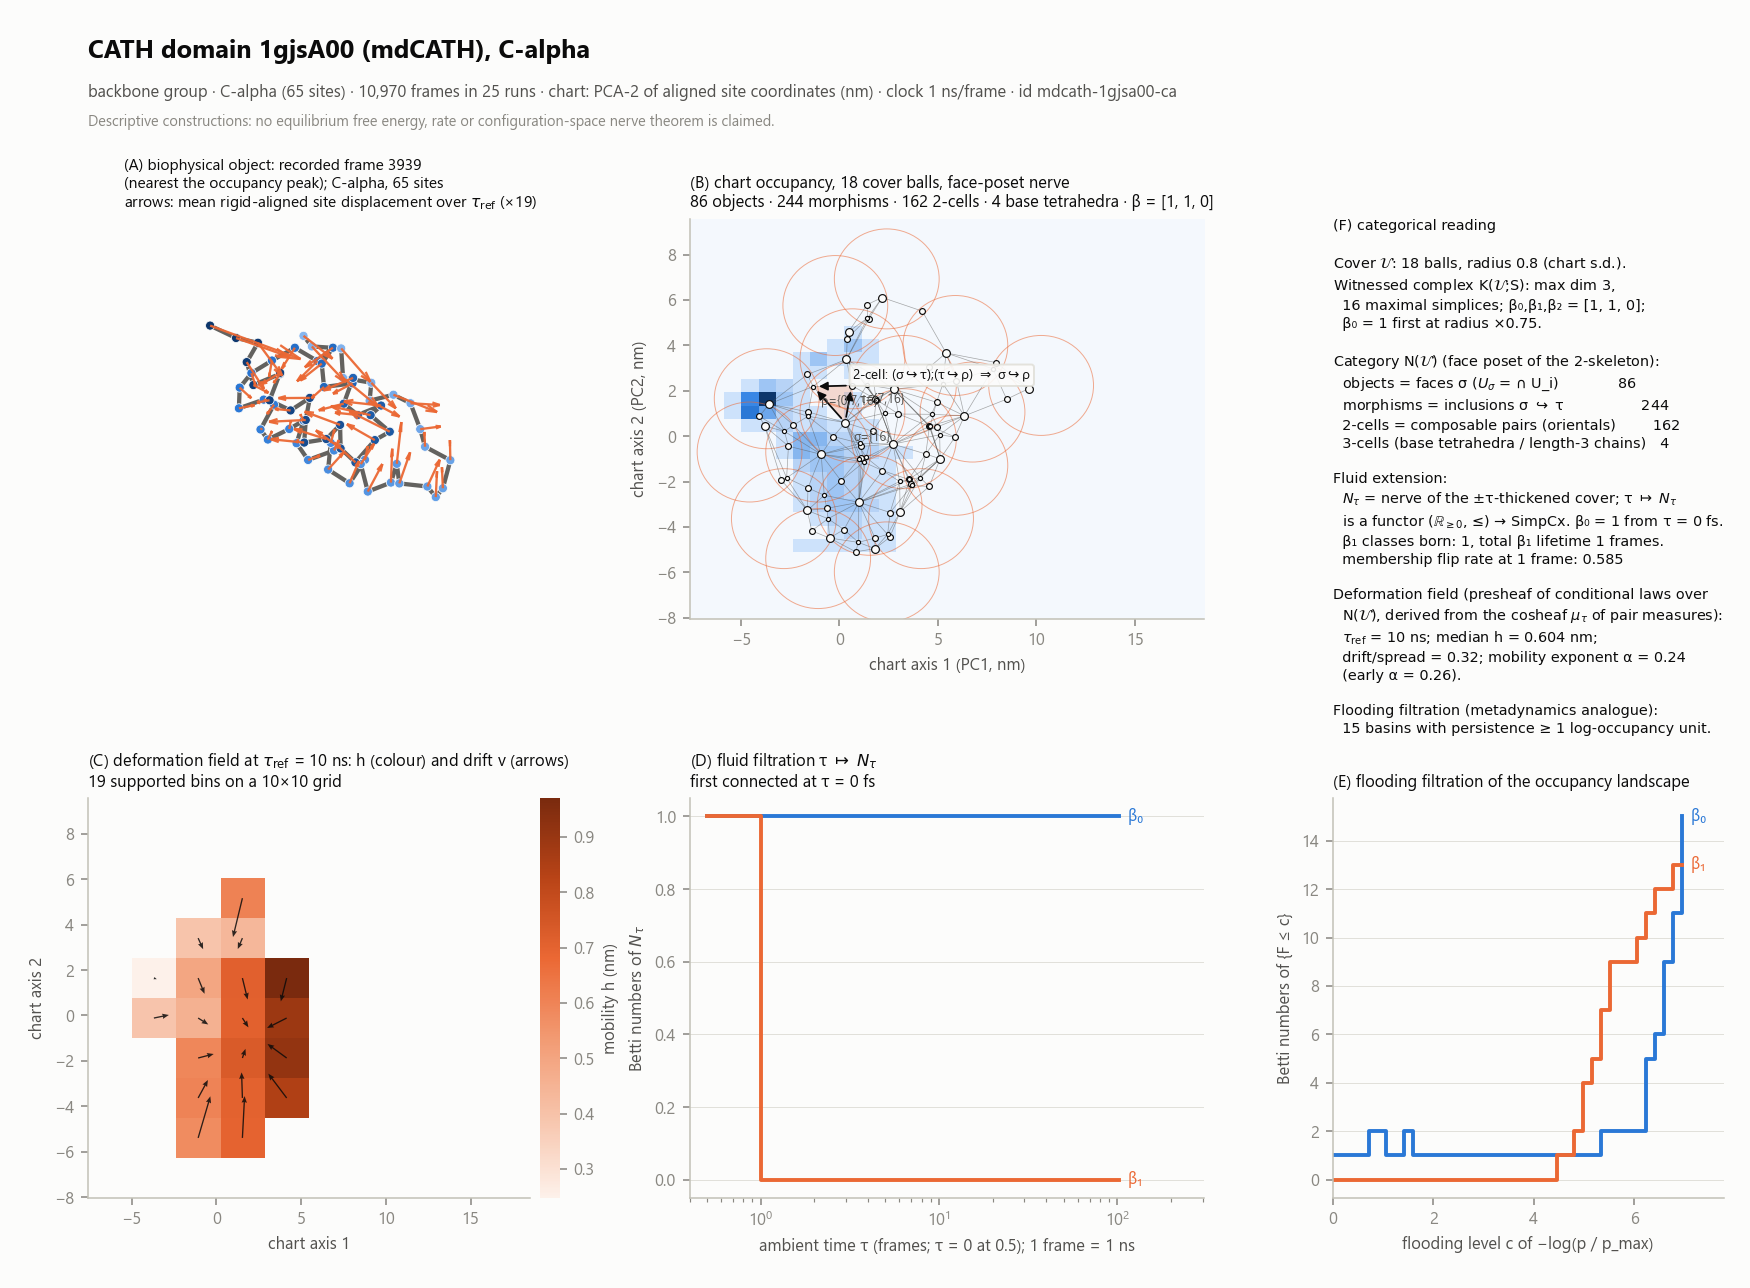
\includegraphics[width=\linewidth,height=.93\textheight,keepaspectratio]{systems/mdcath-1gjsa00-ca/plate.png}\caption{CATH domain 1gjsA00 (mdCATH), C-alpha (\texttt{mdcath-1gjsa00-ca}). Source: https://huggingface.co/datasets/compsciencelab/mdCATH/resolve/main/data/mdcath\_dataset\_1gjsA00.h5.}\end{figure}\clearpage
\begin{figure}[H]\centering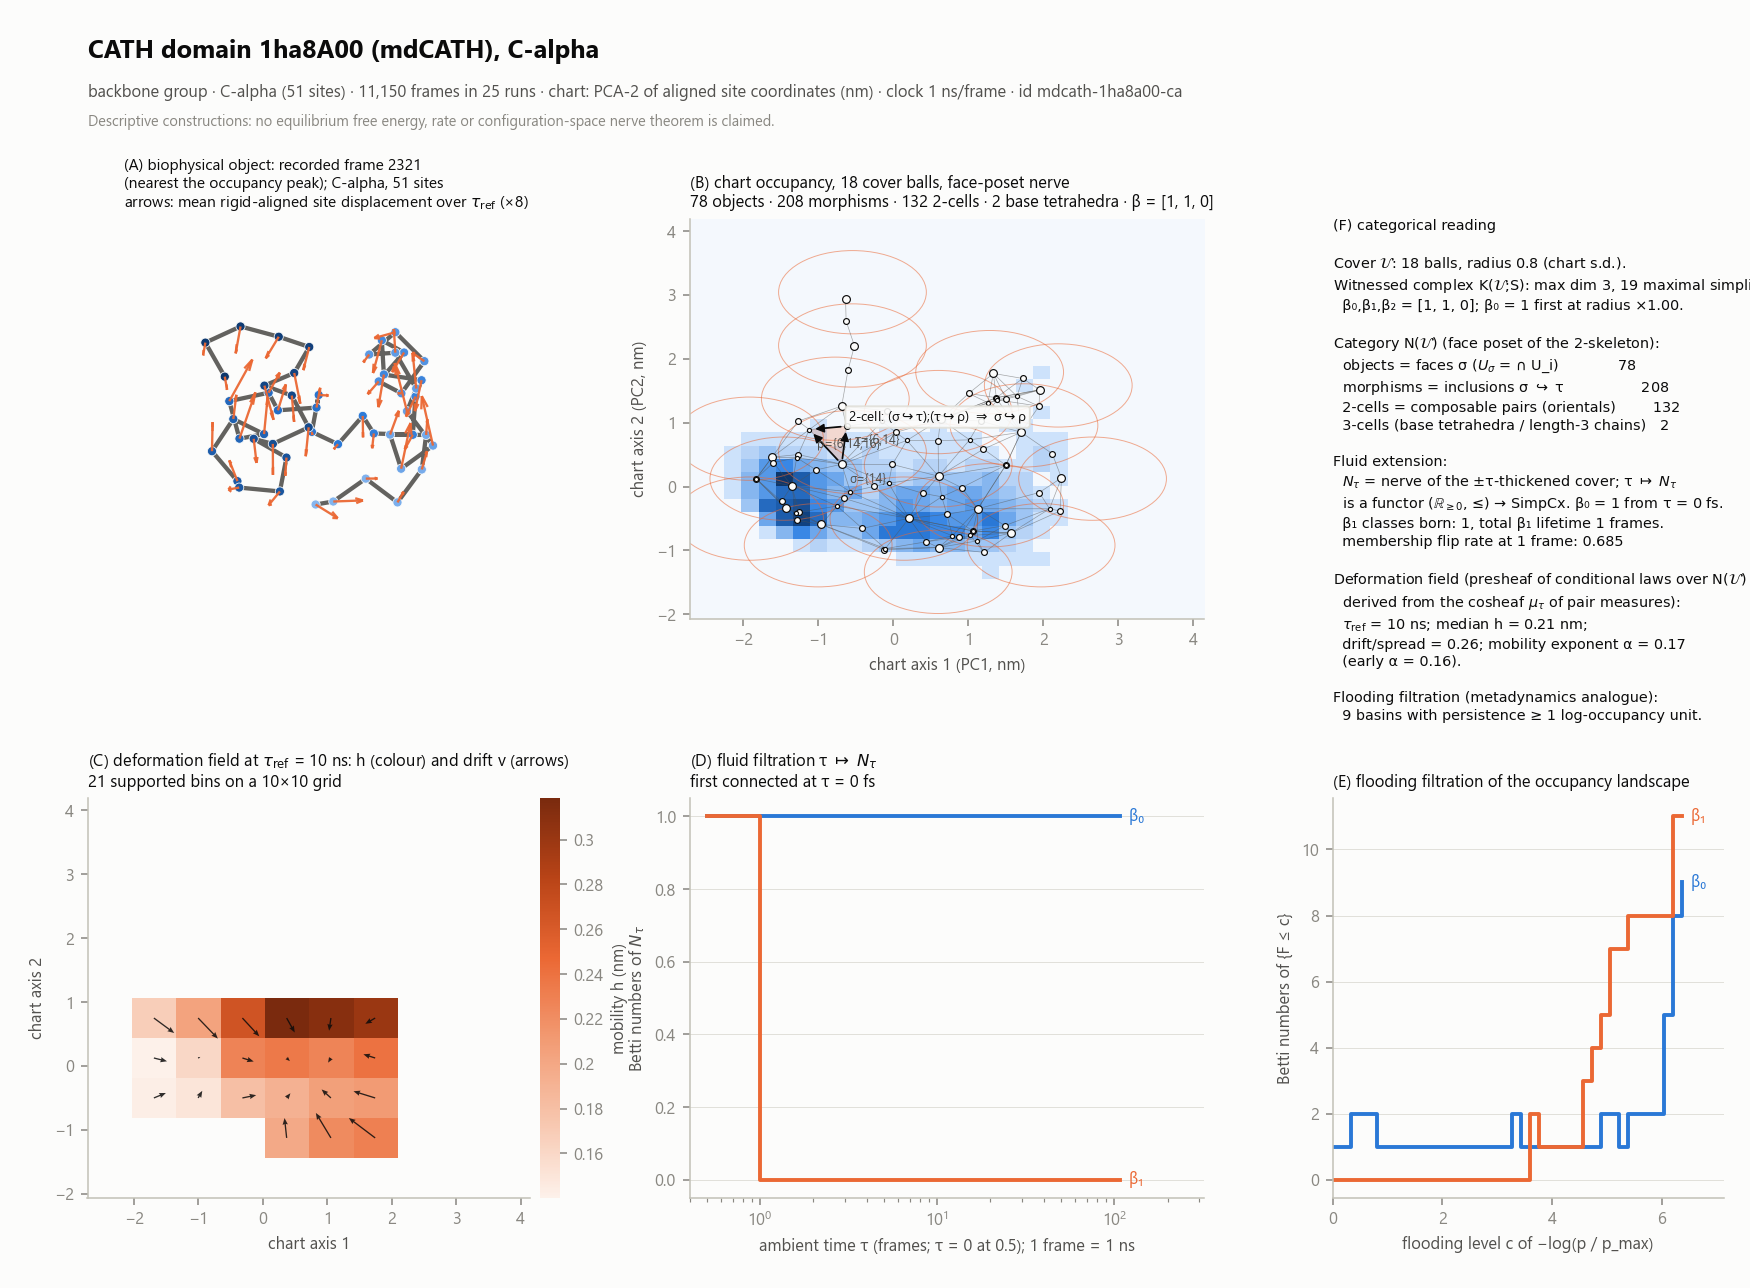
\includegraphics[width=\linewidth,height=.93\textheight,keepaspectratio]{systems/mdcath-1ha8a00-ca/plate.png}\caption{CATH domain 1ha8A00 (mdCATH), C-alpha (\texttt{mdcath-1ha8a00-ca}). Source: https://huggingface.co/datasets/compsciencelab/mdCATH/resolve/main/data/mdcath\_dataset\_1ha8A00.h5.}\end{figure}\clearpage
\begin{figure}[H]\centering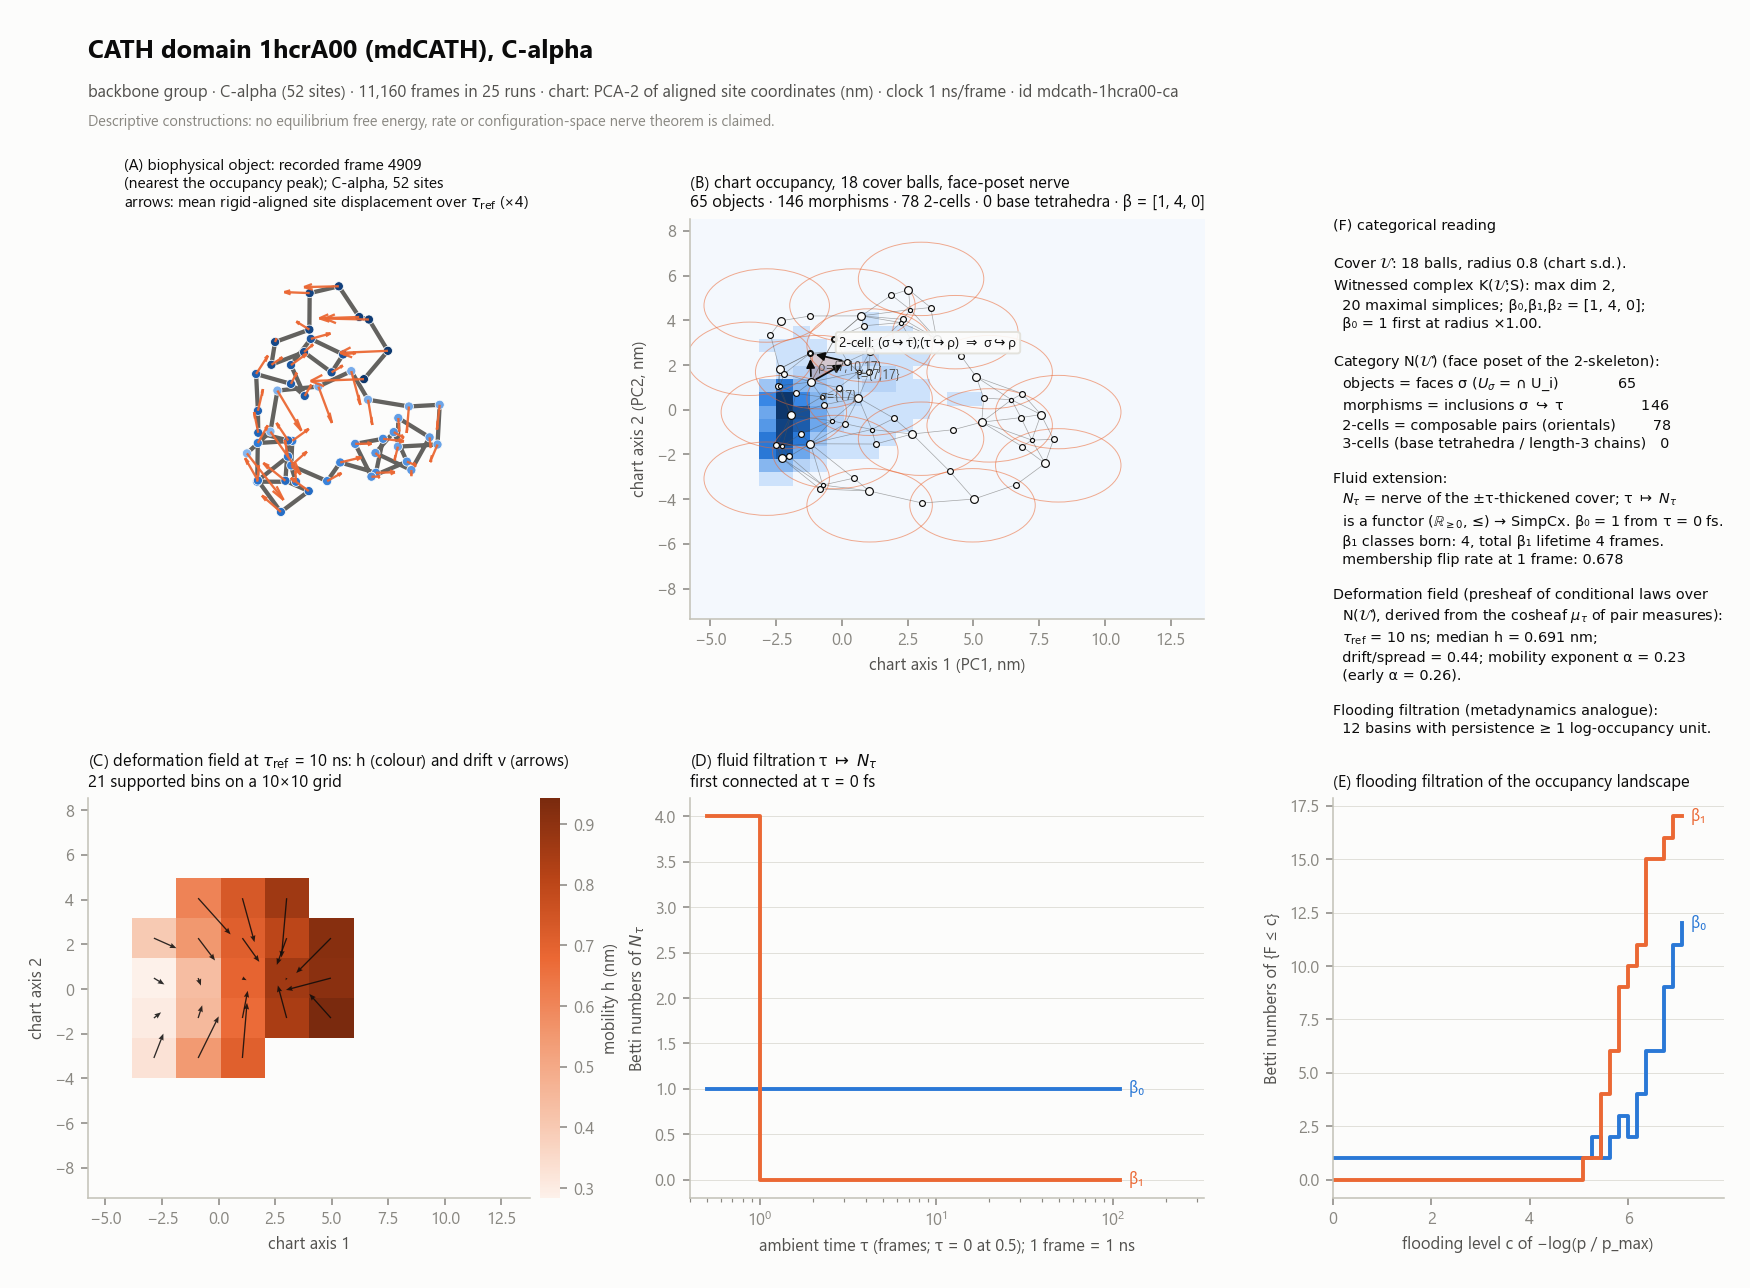
\includegraphics[width=\linewidth,height=.93\textheight,keepaspectratio]{systems/mdcath-1hcra00-ca/plate.png}\caption{CATH domain 1hcrA00 (mdCATH), C-alpha (\texttt{mdcath-1hcra00-ca}). Source: https://huggingface.co/datasets/compsciencelab/mdCATH/resolve/main/data/mdcath\_dataset\_1hcrA00.h5.}\end{figure}\clearpage
\begin{figure}[H]\centering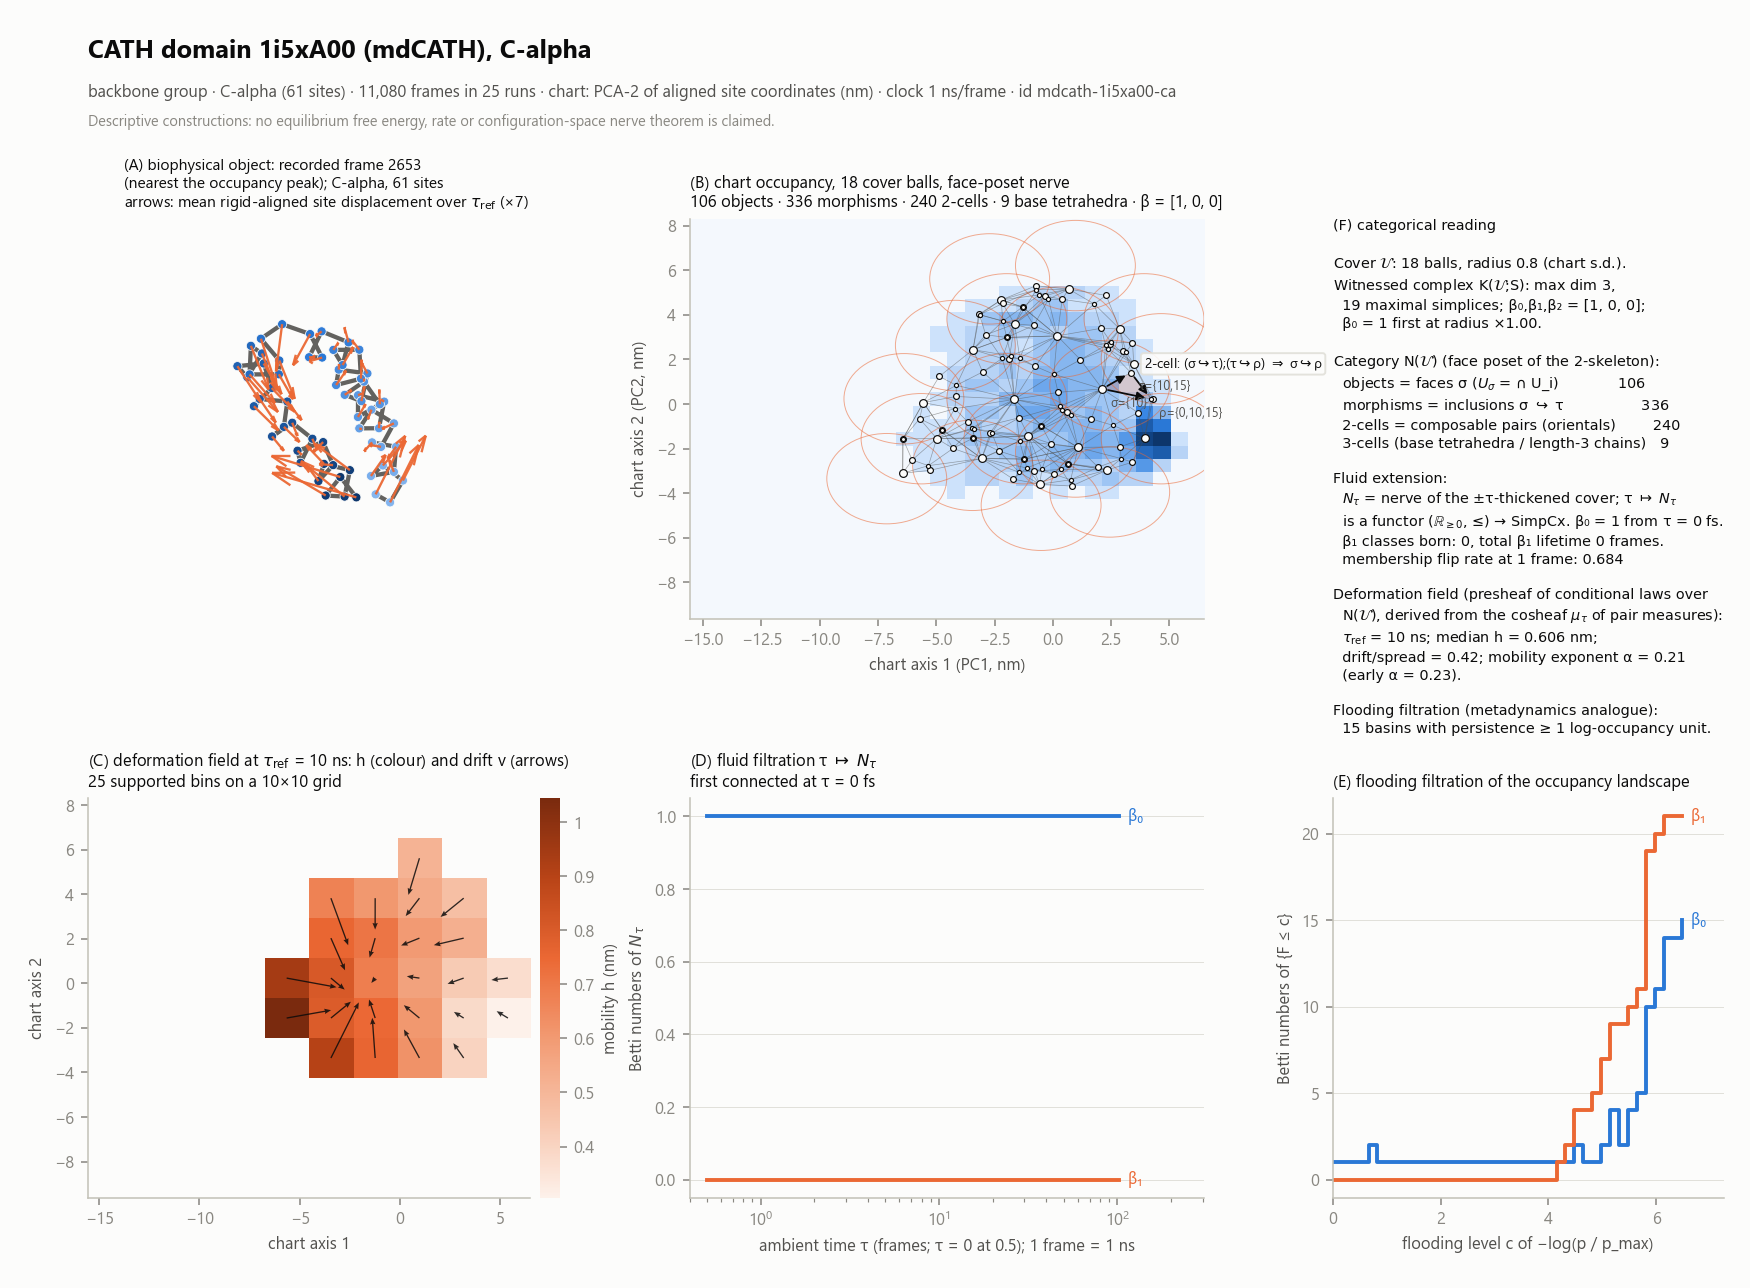
\includegraphics[width=\linewidth,height=.93\textheight,keepaspectratio]{systems/mdcath-1i5xa00-ca/plate.png}\caption{CATH domain 1i5xA00 (mdCATH), C-alpha (\texttt{mdcath-1i5xa00-ca}). Source: https://huggingface.co/datasets/compsciencelab/mdCATH/resolve/main/data/mdcath\_dataset\_1i5xA00.h5.}\end{figure}\clearpage
\begin{figure}[H]\centering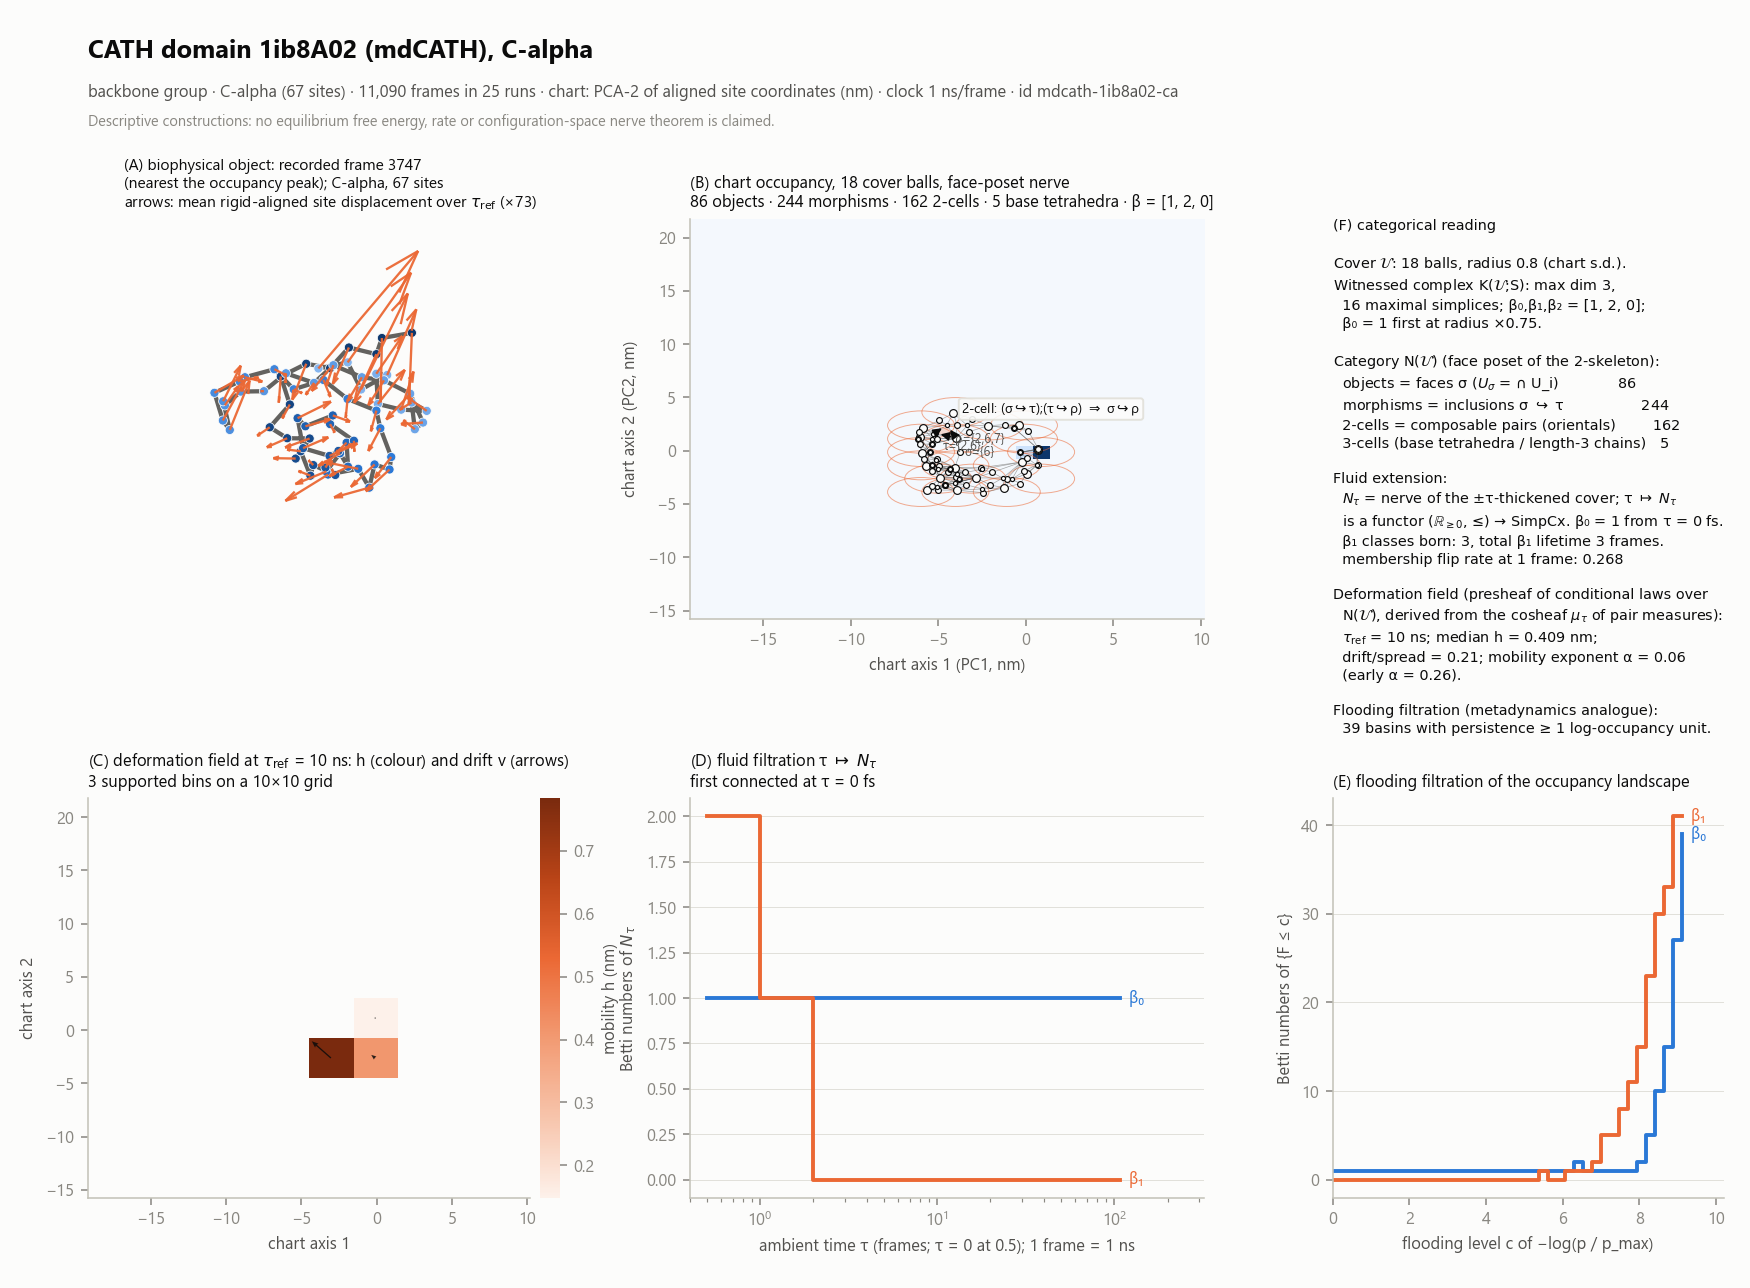
\includegraphics[width=\linewidth,height=.93\textheight,keepaspectratio]{systems/mdcath-1ib8a02-ca/plate.png}\caption{CATH domain 1ib8A02 (mdCATH), C-alpha (\texttt{mdcath-1ib8a02-ca}). Source: https://huggingface.co/datasets/compsciencelab/mdCATH/resolve/main/data/mdcath\_dataset\_1ib8A02.h5.}\end{figure}\clearpage
\begin{figure}[H]\centering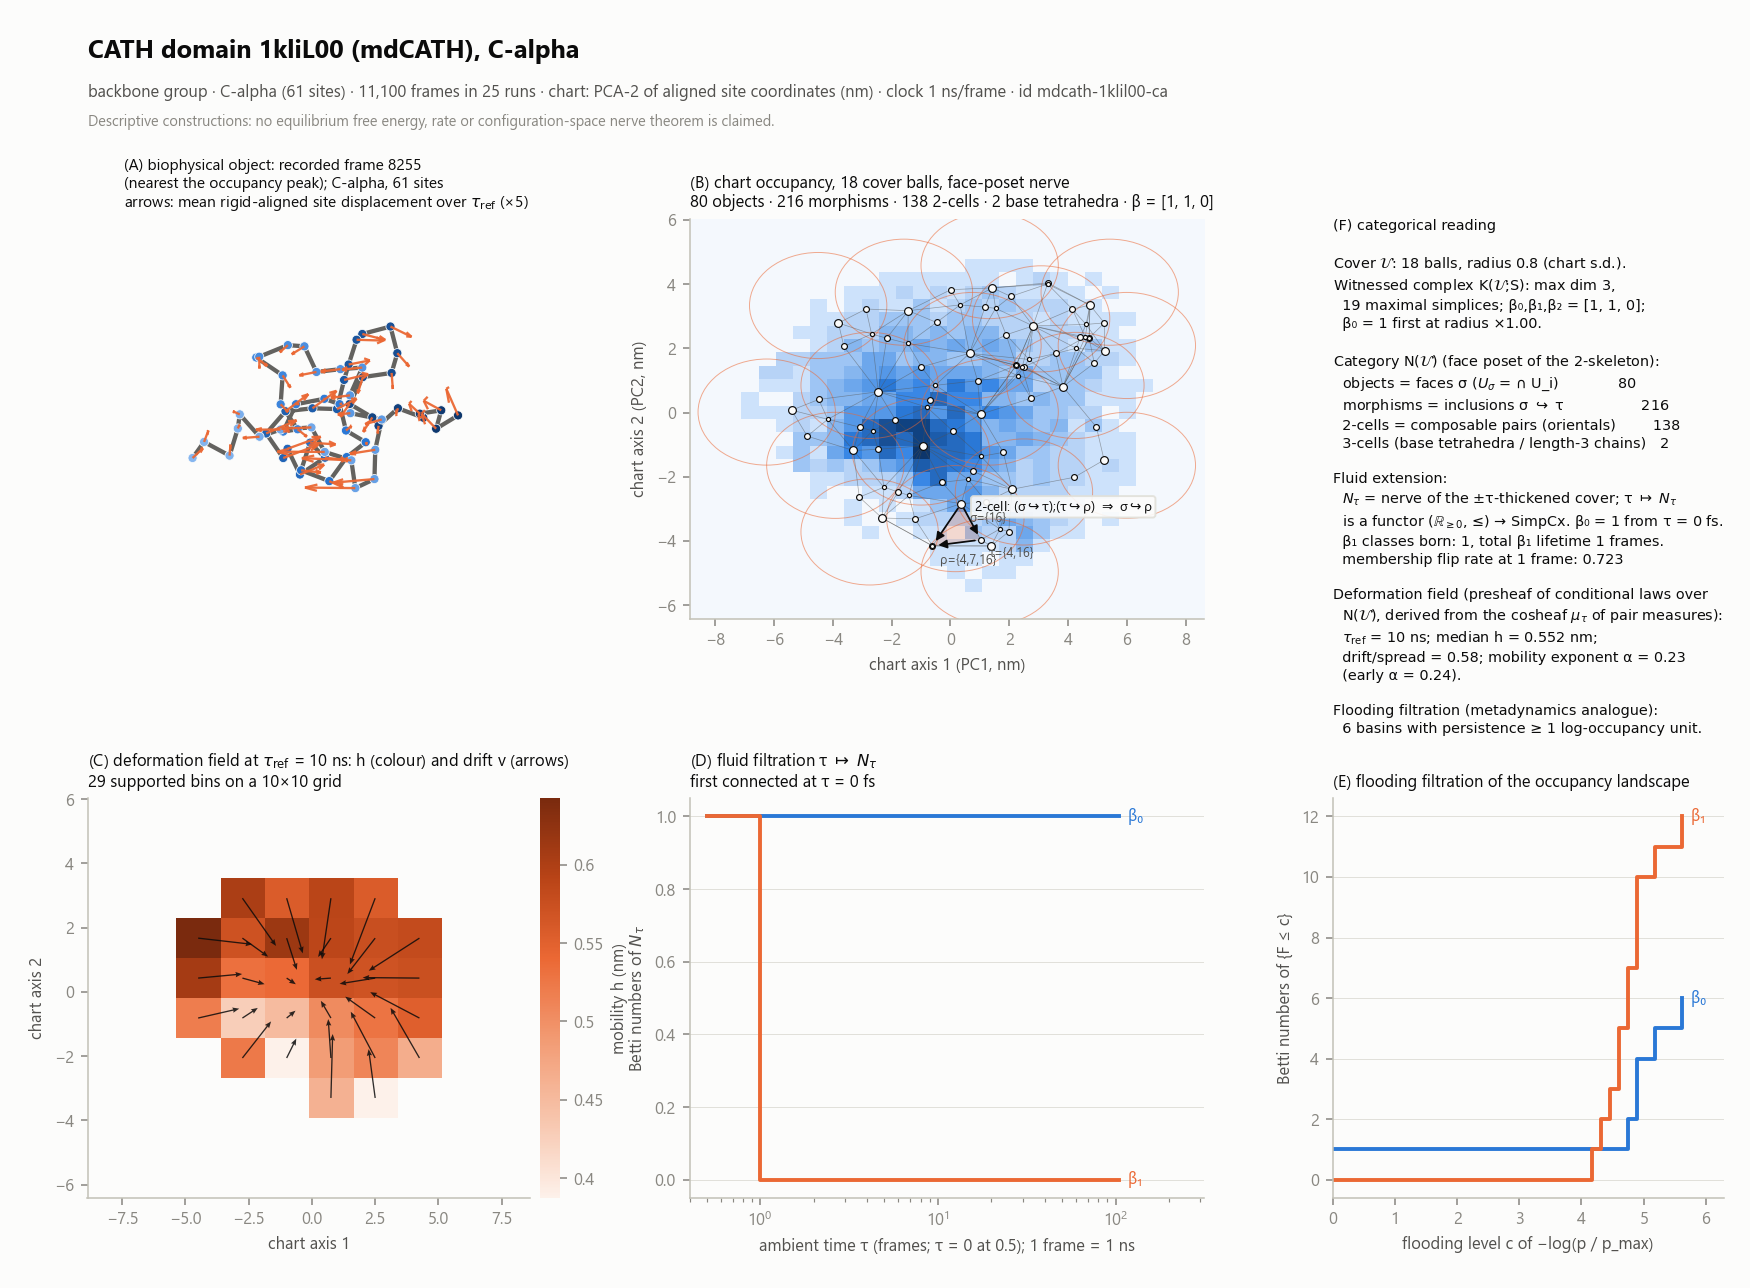
\includegraphics[width=\linewidth,height=.93\textheight,keepaspectratio]{systems/mdcath-1klil00-ca/plate.png}\caption{CATH domain 1kliL00 (mdCATH), C-alpha (\texttt{mdcath-1klil00-ca}). Source: https://huggingface.co/datasets/compsciencelab/mdCATH/resolve/main/data/mdcath\_dataset\_1kliL00.h5.}\end{figure}\clearpage
\begin{figure}[H]\centering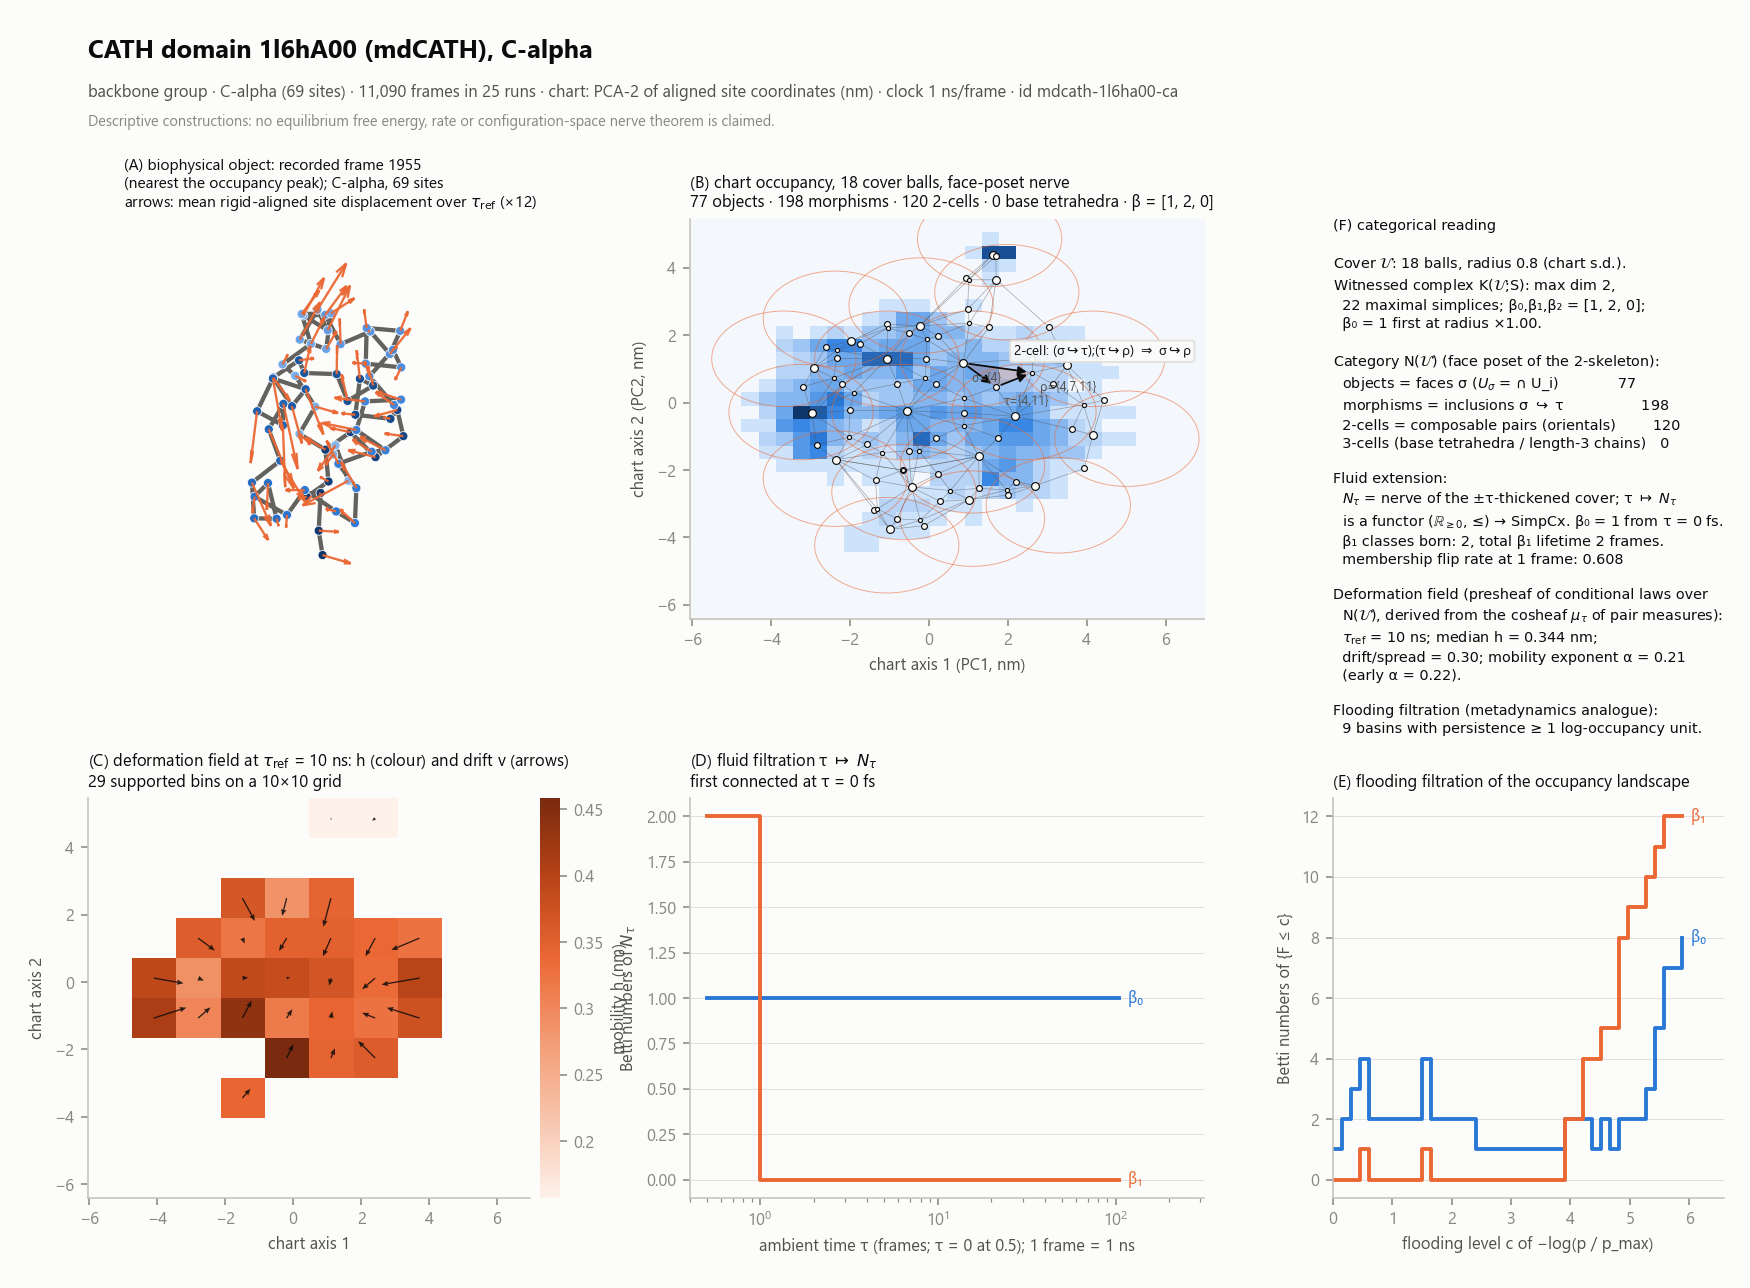
\includegraphics[width=\linewidth,height=.93\textheight,keepaspectratio]{systems/mdcath-1l6ha00-ca/plate.png}\caption{CATH domain 1l6hA00 (mdCATH), C-alpha (\texttt{mdcath-1l6ha00-ca}). Source: https://huggingface.co/datasets/compsciencelab/mdCATH/resolve/main/data/mdcath\_dataset\_1l6hA00.h5.}\end{figure}\clearpage
\begin{figure}[H]\centering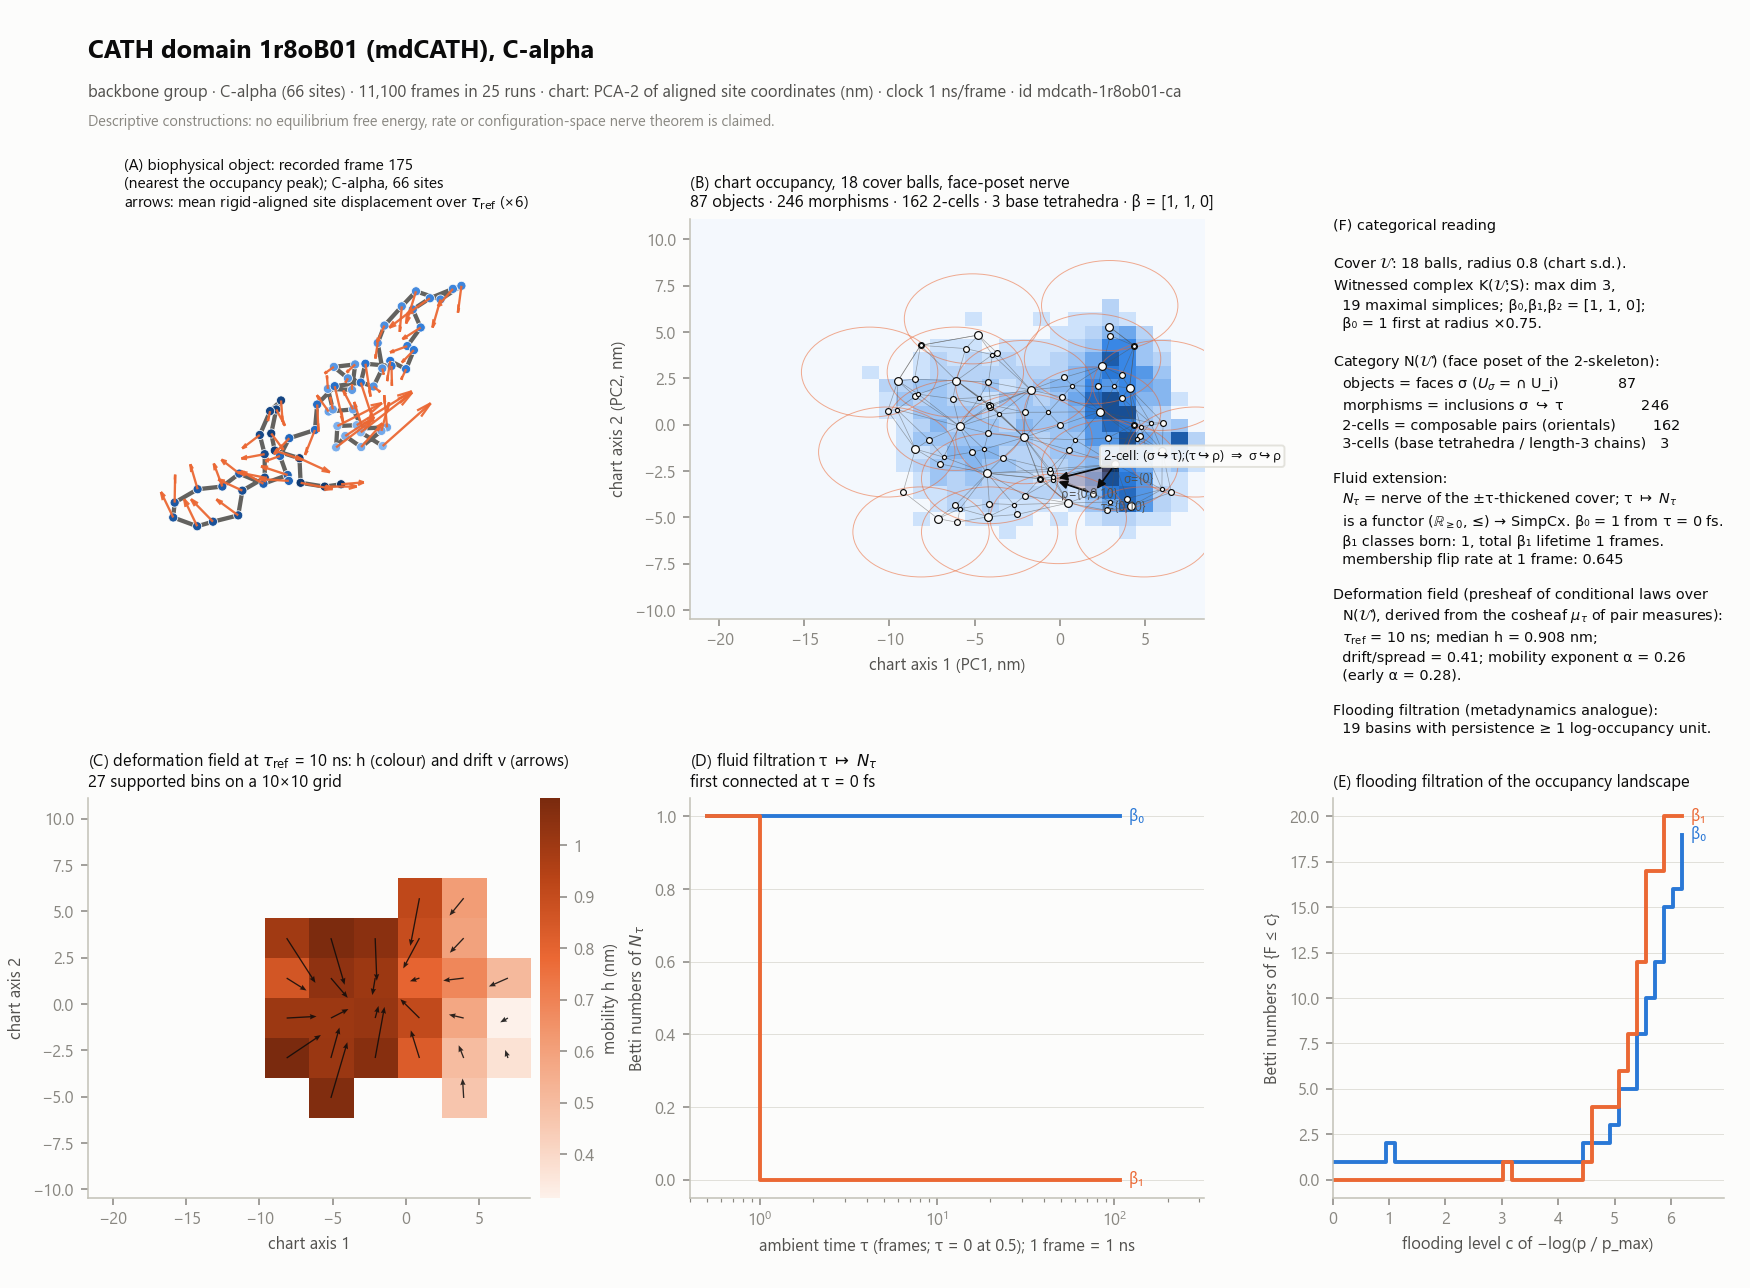
\includegraphics[width=\linewidth,height=.93\textheight,keepaspectratio]{systems/mdcath-1r8ob01-ca/plate.png}\caption{CATH domain 1r8oB01 (mdCATH), C-alpha (\texttt{mdcath-1r8ob01-ca}). Source: https://huggingface.co/datasets/compsciencelab/mdCATH/resolve/main/data/mdcath\_dataset\_1r8oB01.h5.}\end{figure}\clearpage
\begin{figure}[H]\centering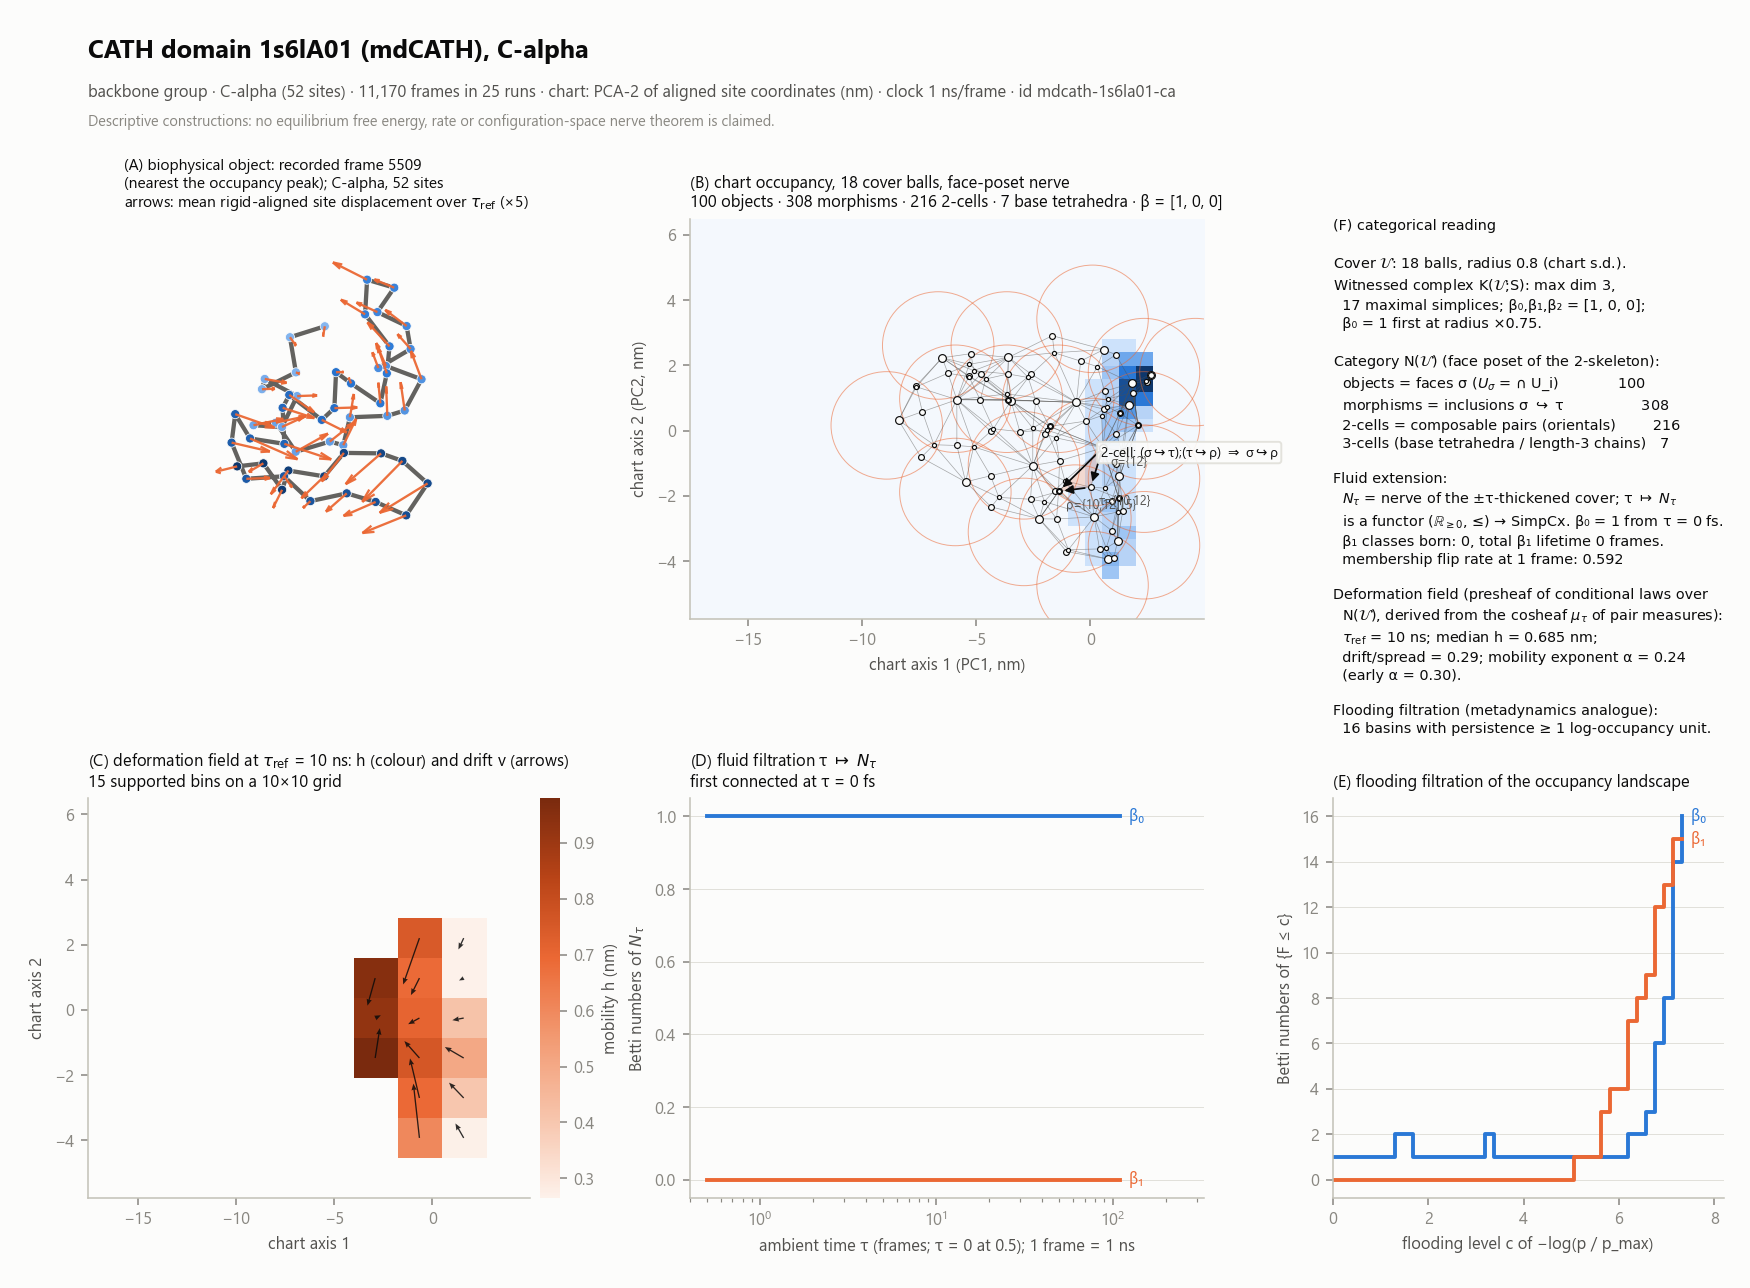
\includegraphics[width=\linewidth,height=.93\textheight,keepaspectratio]{systems/mdcath-1s6la01-ca/plate.png}\caption{CATH domain 1s6lA01 (mdCATH), C-alpha (\texttt{mdcath-1s6la01-ca}). Source: https://huggingface.co/datasets/compsciencelab/mdCATH/resolve/main/data/mdcath\_dataset\_1s6lA01.h5.}\end{figure}\clearpage
\begin{figure}[H]\centering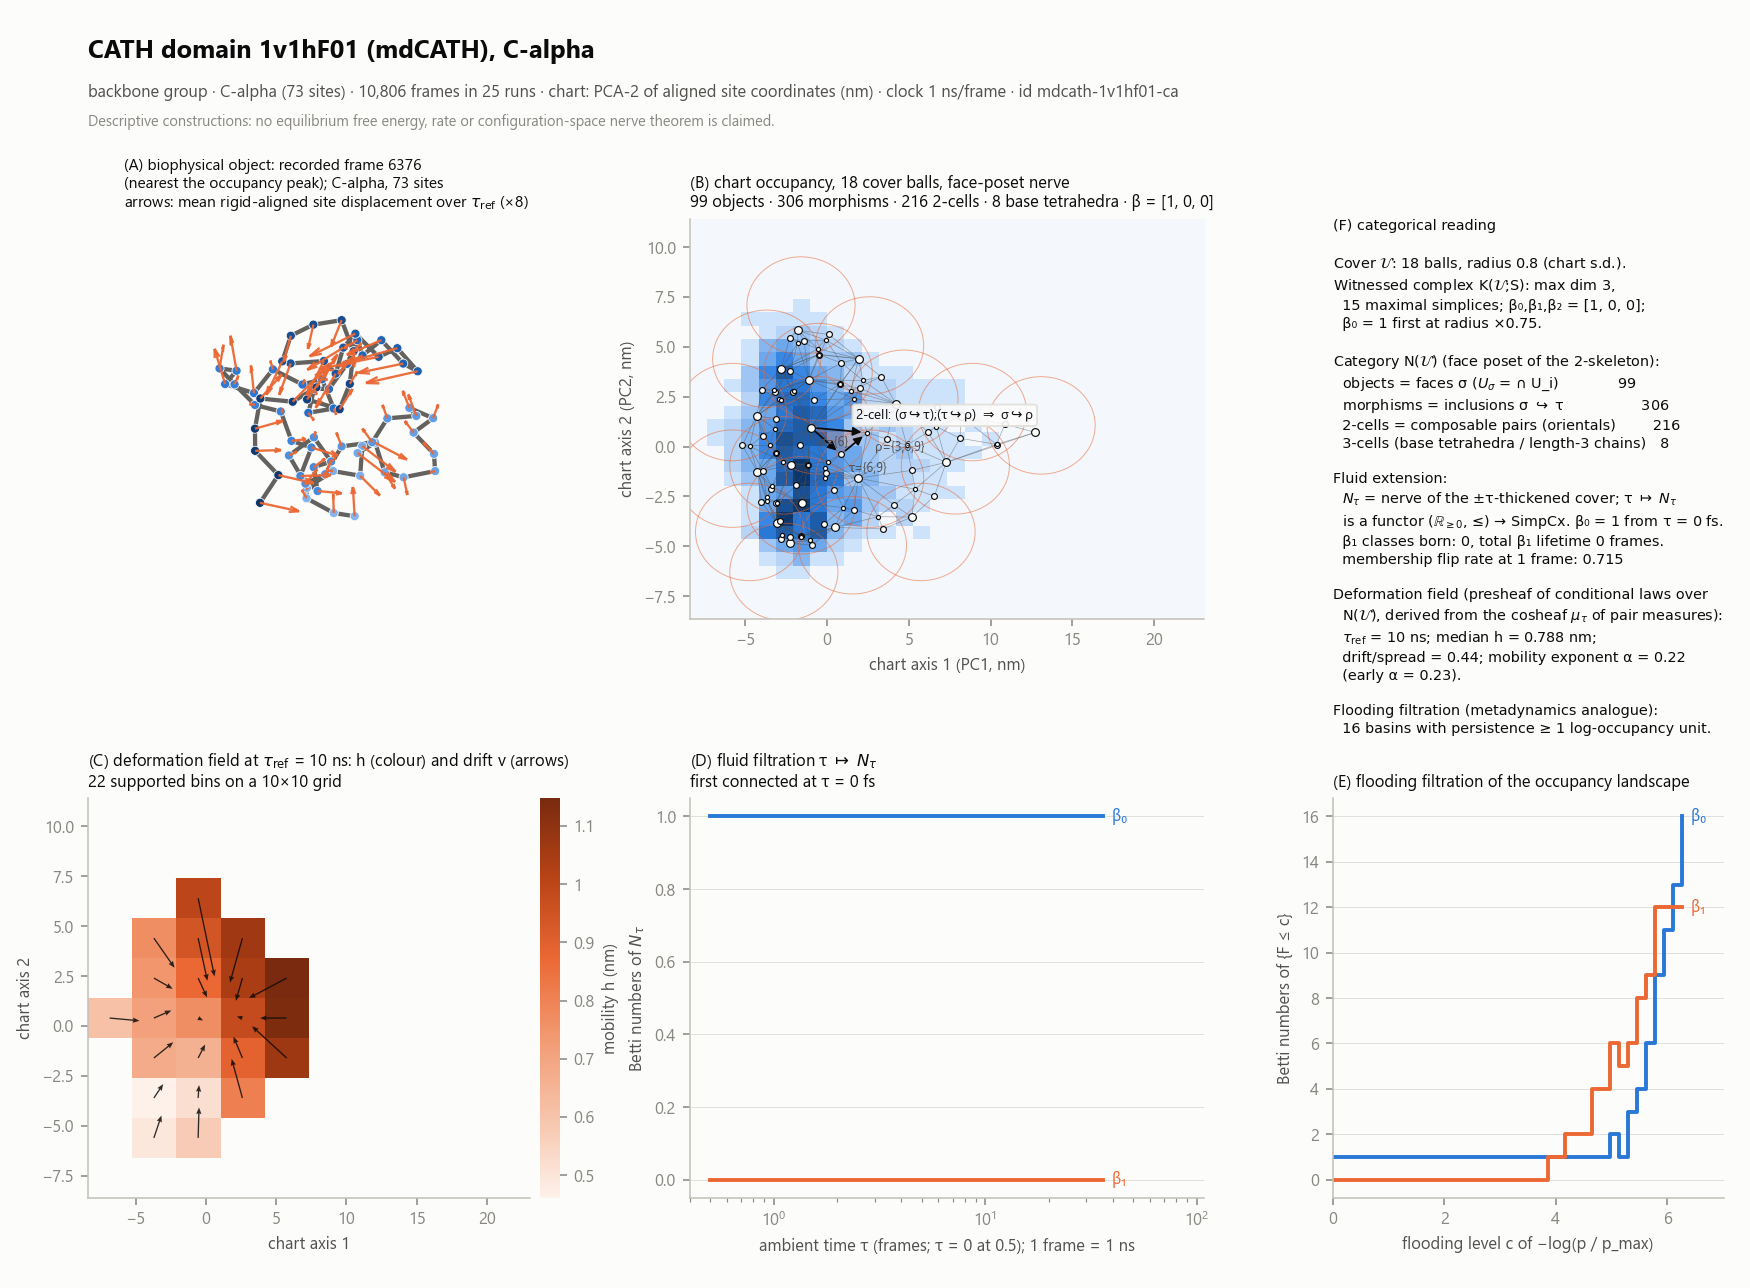
\includegraphics[width=\linewidth,height=.93\textheight,keepaspectratio]{systems/mdcath-1v1hf01-ca/plate.png}\caption{CATH domain 1v1hF01 (mdCATH), C-alpha (\texttt{mdcath-1v1hf01-ca}). Source: https://huggingface.co/datasets/compsciencelab/mdCATH/resolve/main/data/mdcath\_dataset\_1v1hF01.h5.}\end{figure}\clearpage
\begin{figure}[H]\centering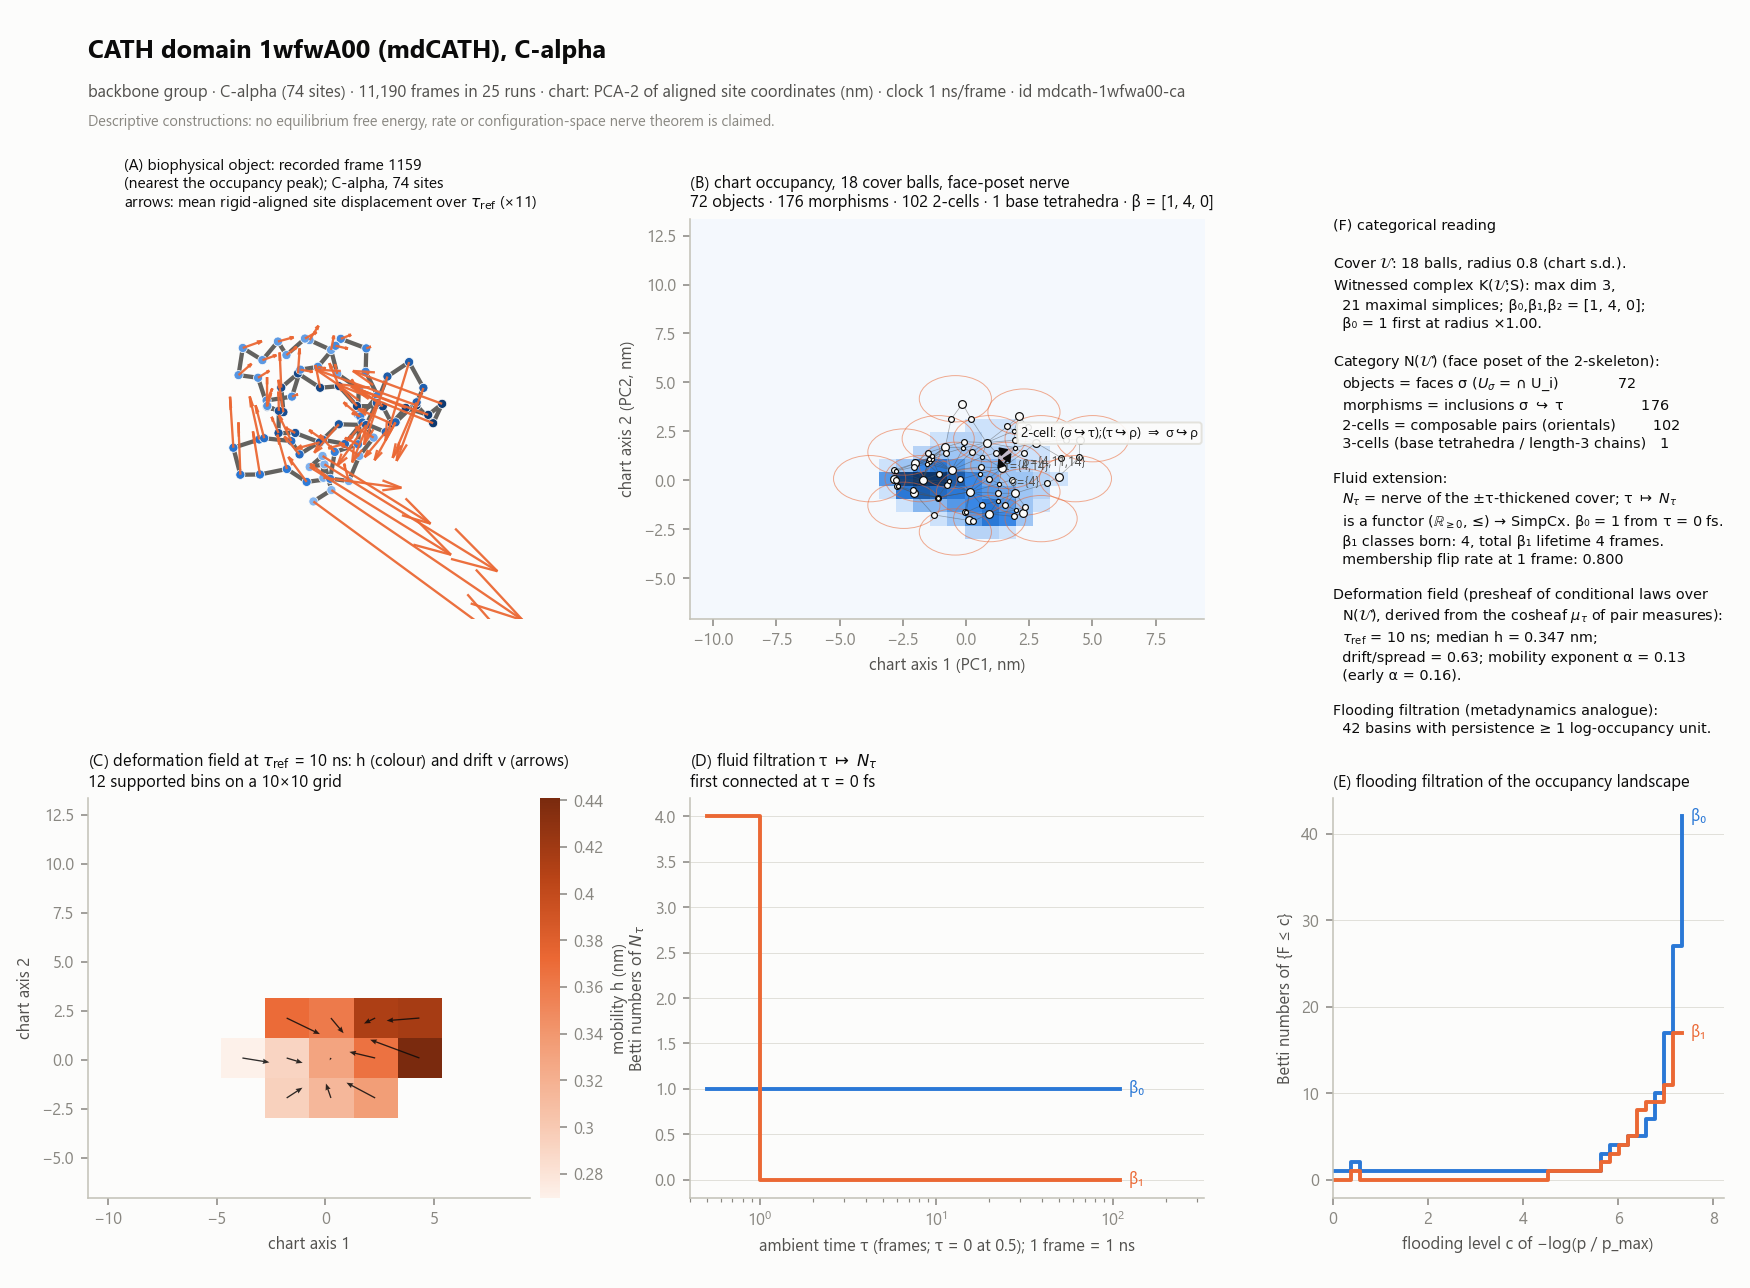
\includegraphics[width=\linewidth,height=.93\textheight,keepaspectratio]{systems/mdcath-1wfwa00-ca/plate.png}\caption{CATH domain 1wfwA00 (mdCATH), C-alpha (\texttt{mdcath-1wfwa00-ca}). Source: https://huggingface.co/datasets/compsciencelab/mdCATH/resolve/main/data/mdcath\_dataset\_1wfwA00.h5.}\end{figure}\clearpage
\begin{figure}[H]\centering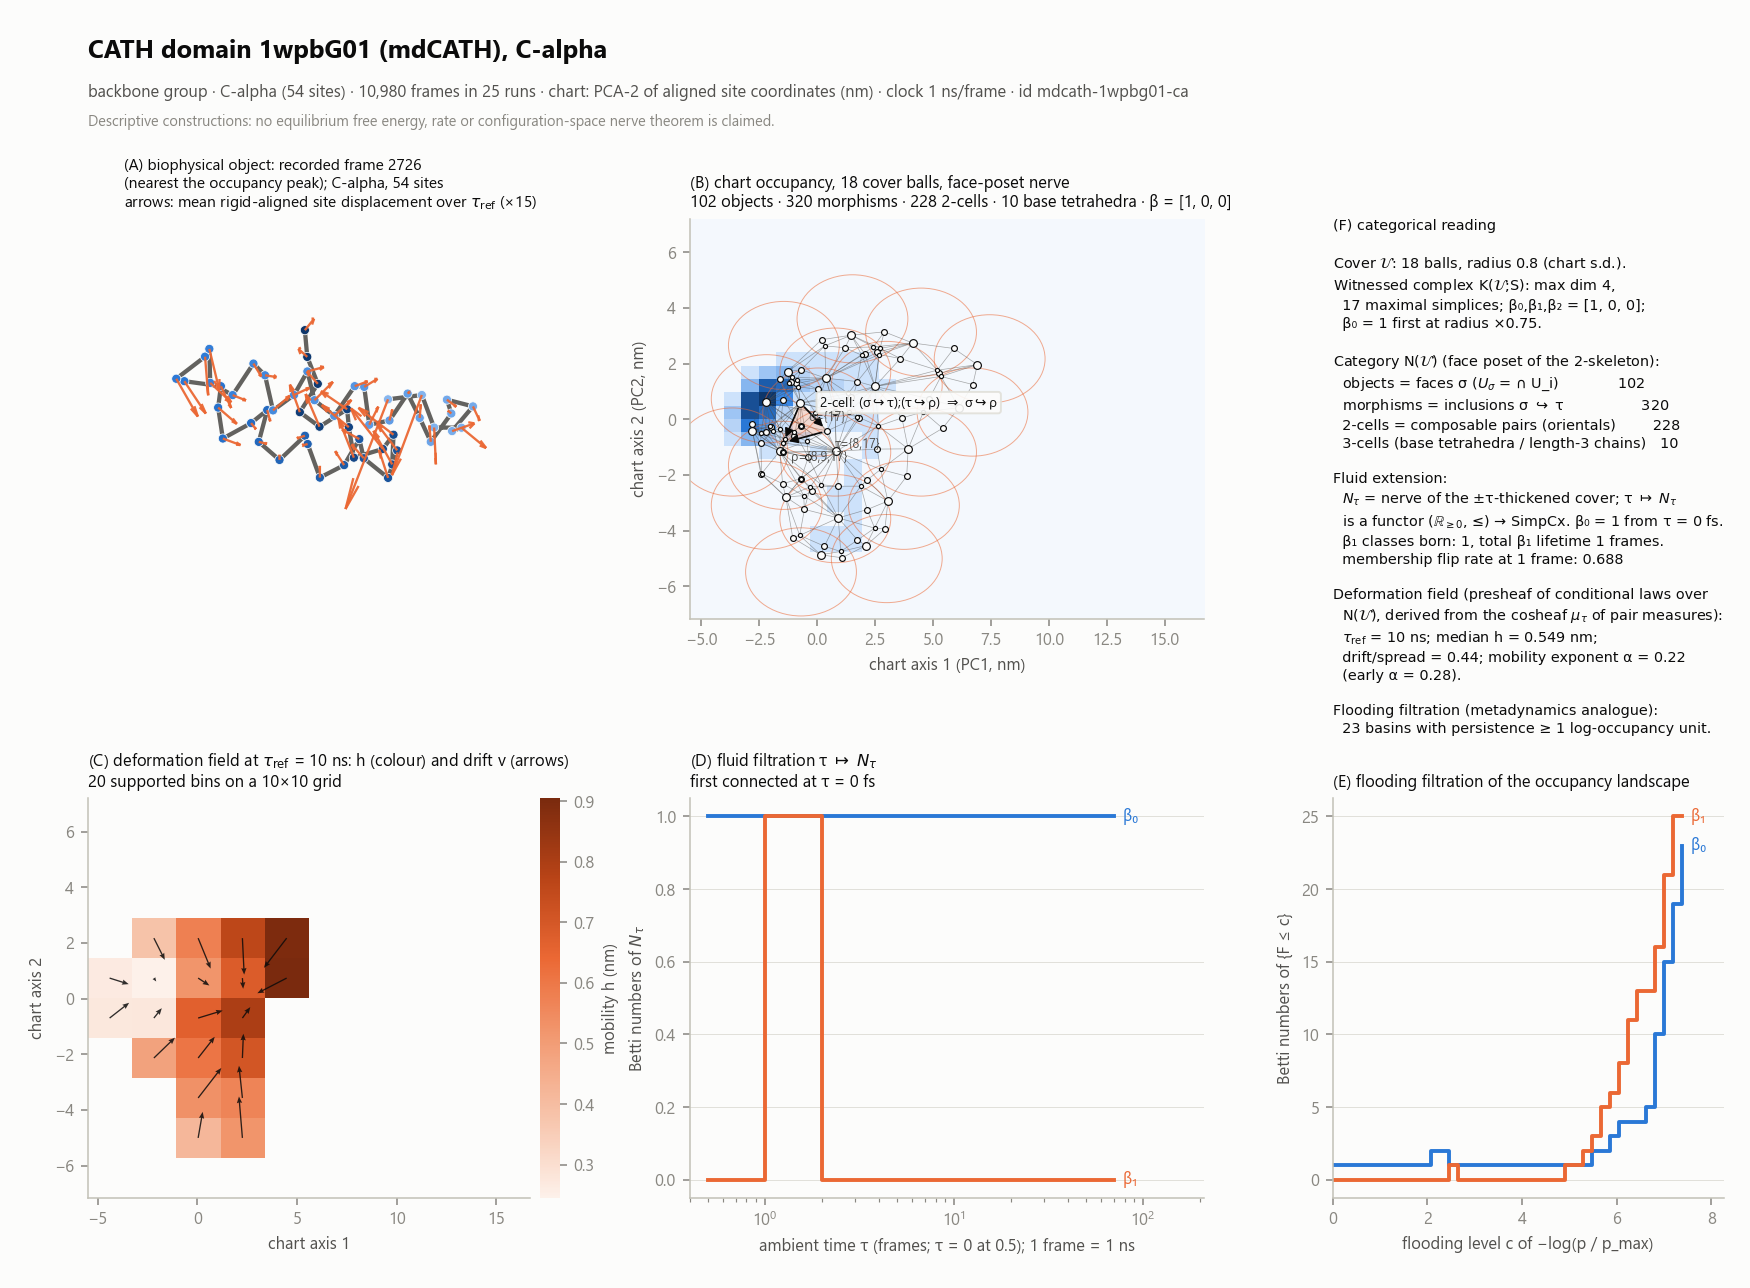
\includegraphics[width=\linewidth,height=.93\textheight,keepaspectratio]{systems/mdcath-1wpbg01-ca/plate.png}\caption{CATH domain 1wpbG01 (mdCATH), C-alpha (\texttt{mdcath-1wpbg01-ca}). Source: https://huggingface.co/datasets/compsciencelab/mdCATH/resolve/main/data/mdcath\_dataset\_1wpbG01.h5.}\end{figure}\clearpage
\begin{figure}[H]\centering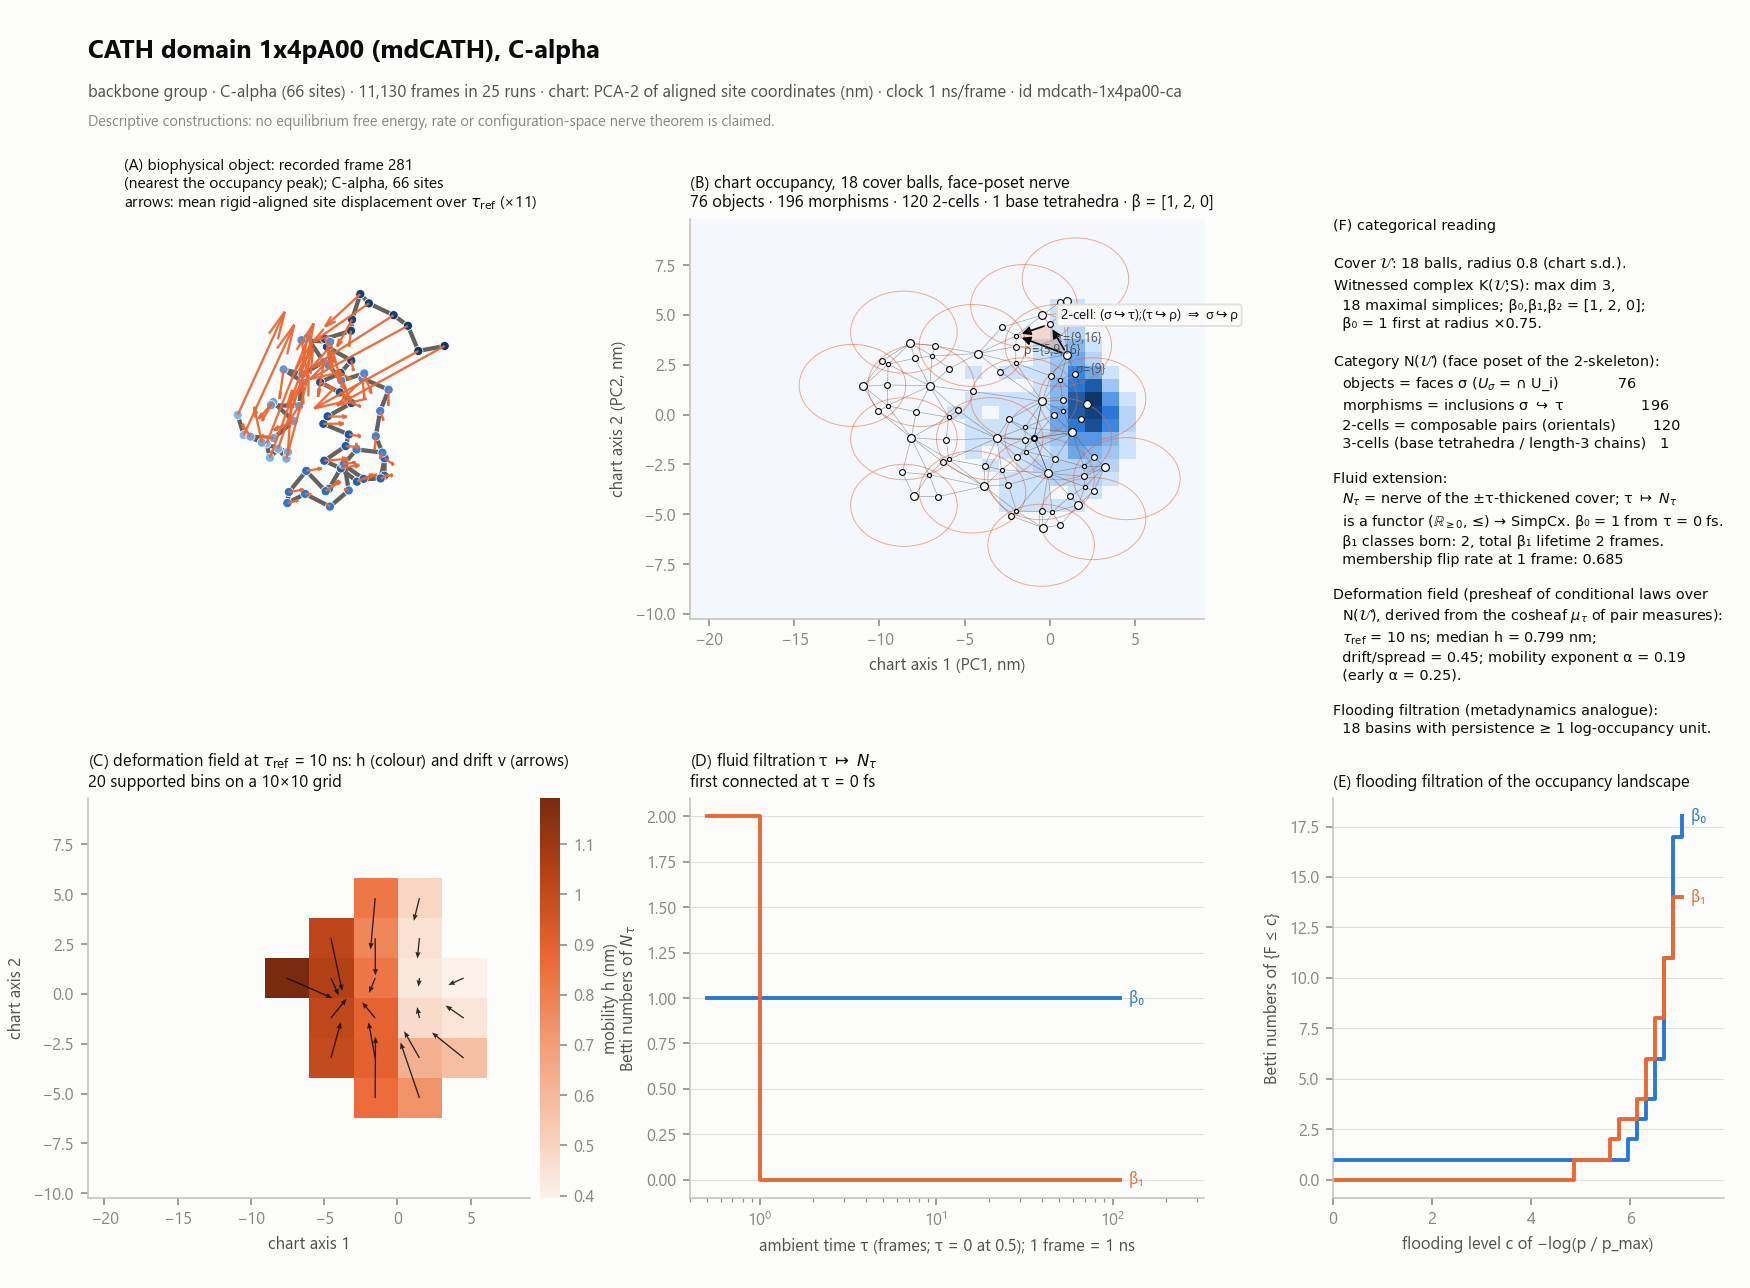
\includegraphics[width=\linewidth,height=.93\textheight,keepaspectratio]{systems/mdcath-1x4pa00-ca/plate.png}\caption{CATH domain 1x4pA00 (mdCATH), C-alpha (\texttt{mdcath-1x4pa00-ca}). Source: https://huggingface.co/datasets/compsciencelab/mdCATH/resolve/main/data/mdcath\_dataset\_1x4pA00.h5.}\end{figure}\clearpage
\begin{figure}[H]\centering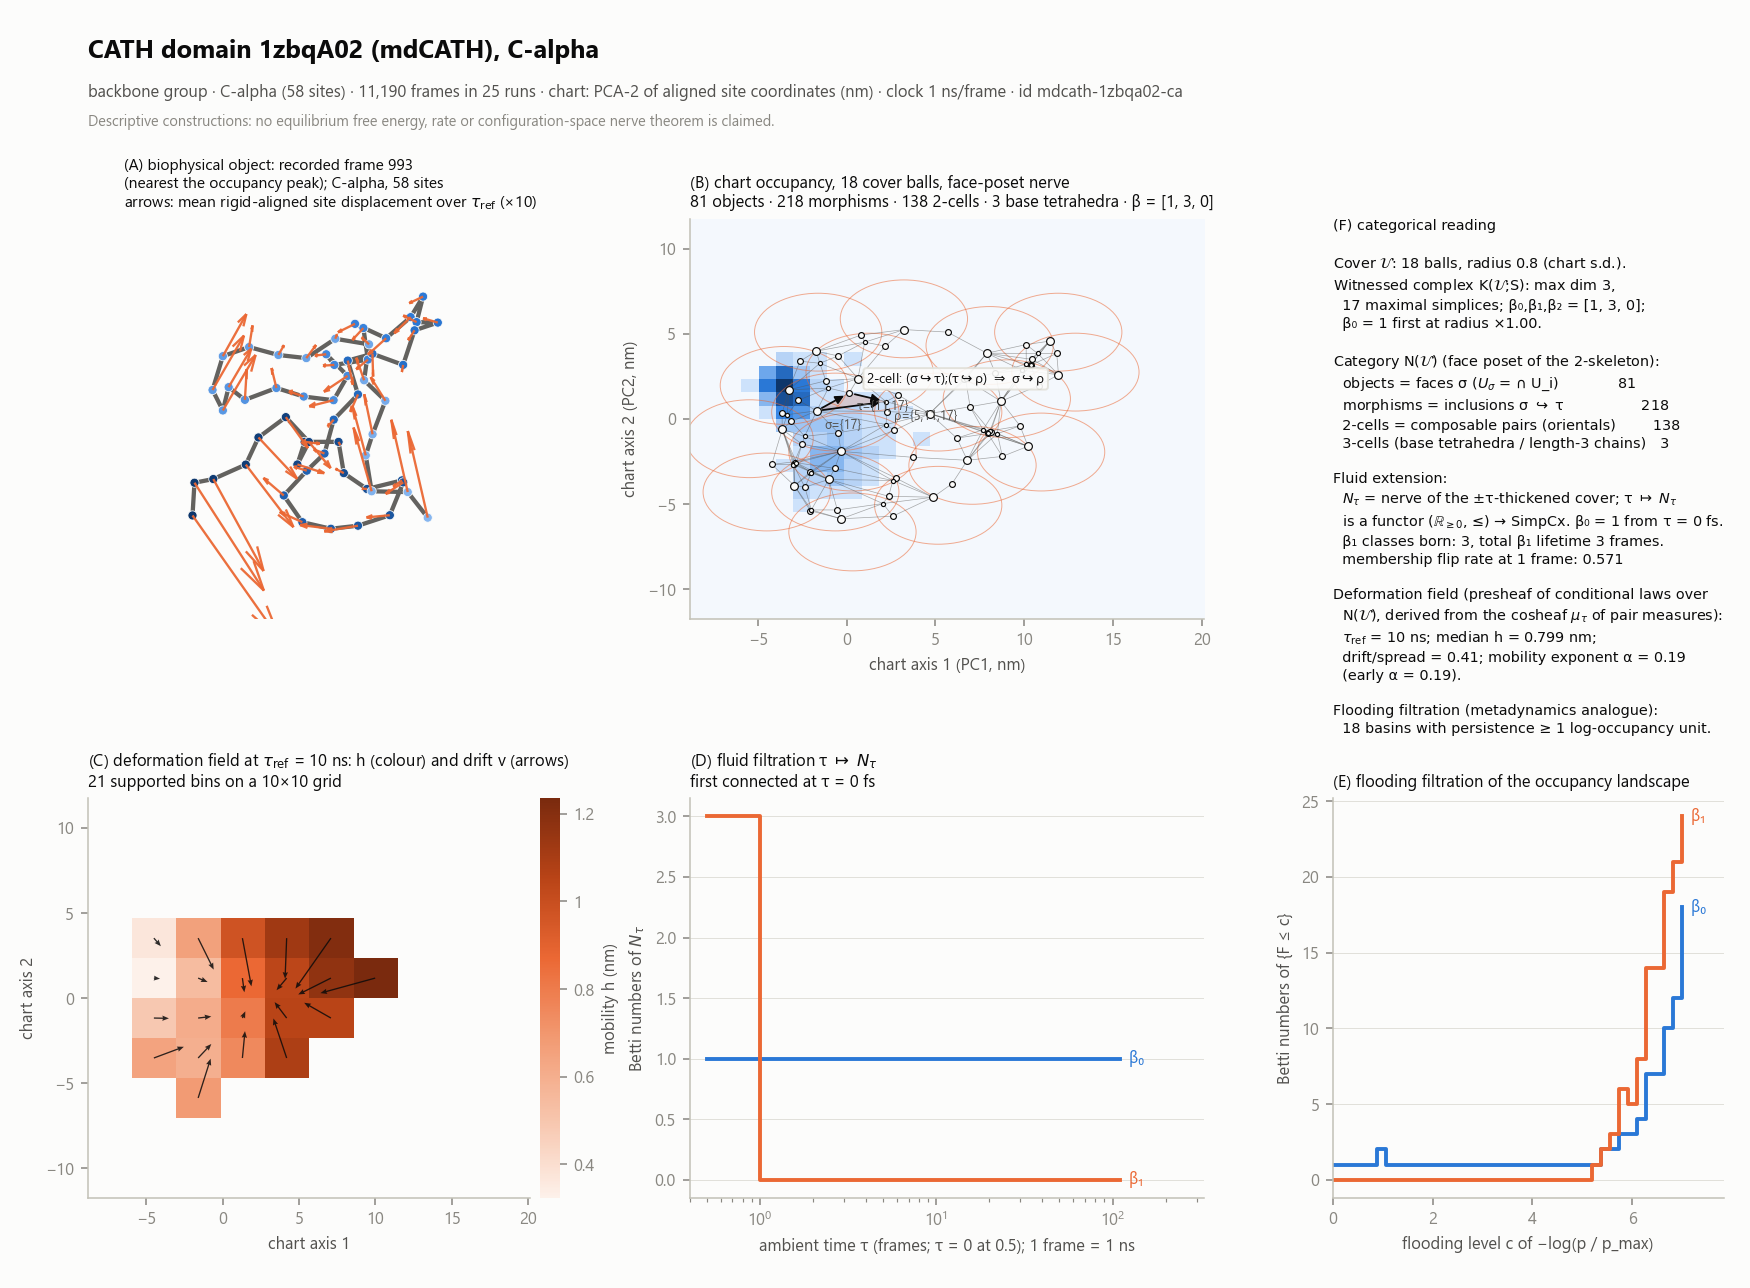
\includegraphics[width=\linewidth,height=.93\textheight,keepaspectratio]{systems/mdcath-1zbqa02-ca/plate.png}\caption{CATH domain 1zbqA02 (mdCATH), C-alpha (\texttt{mdcath-1zbqa02-ca}). Source: https://huggingface.co/datasets/compsciencelab/mdCATH/resolve/main/data/mdcath\_dataset\_1zbqA02.h5.}\end{figure}\clearpage
\begin{figure}[H]\centering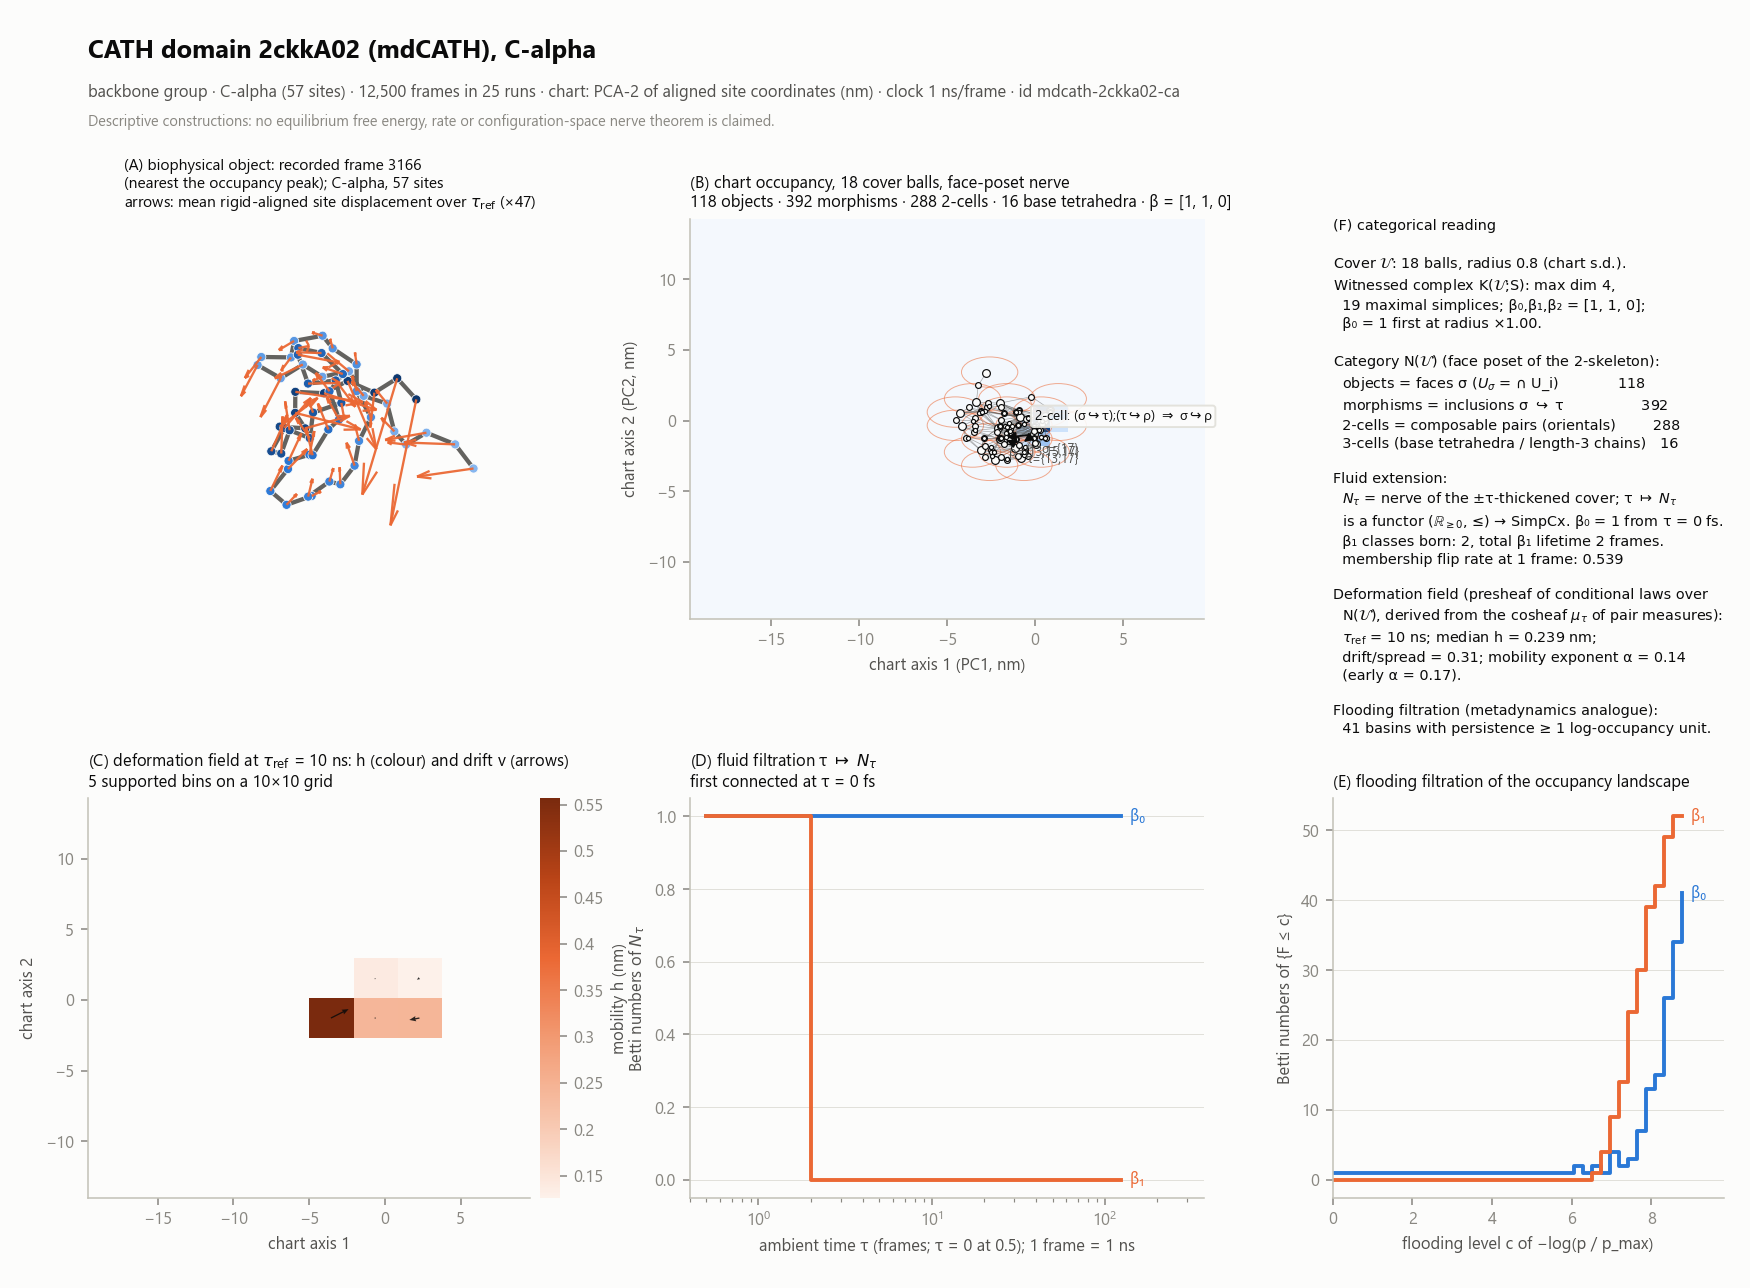
\includegraphics[width=\linewidth,height=.93\textheight,keepaspectratio]{systems/mdcath-2ckka02-ca/plate.png}\caption{CATH domain 2ckkA02 (mdCATH), C-alpha (\texttt{mdcath-2ckka02-ca}). Source: https://huggingface.co/datasets/compsciencelab/mdCATH/resolve/main/data/mdcath\_dataset\_2ckkA02.h5.}\end{figure}\clearpage
\begin{figure}[H]\centering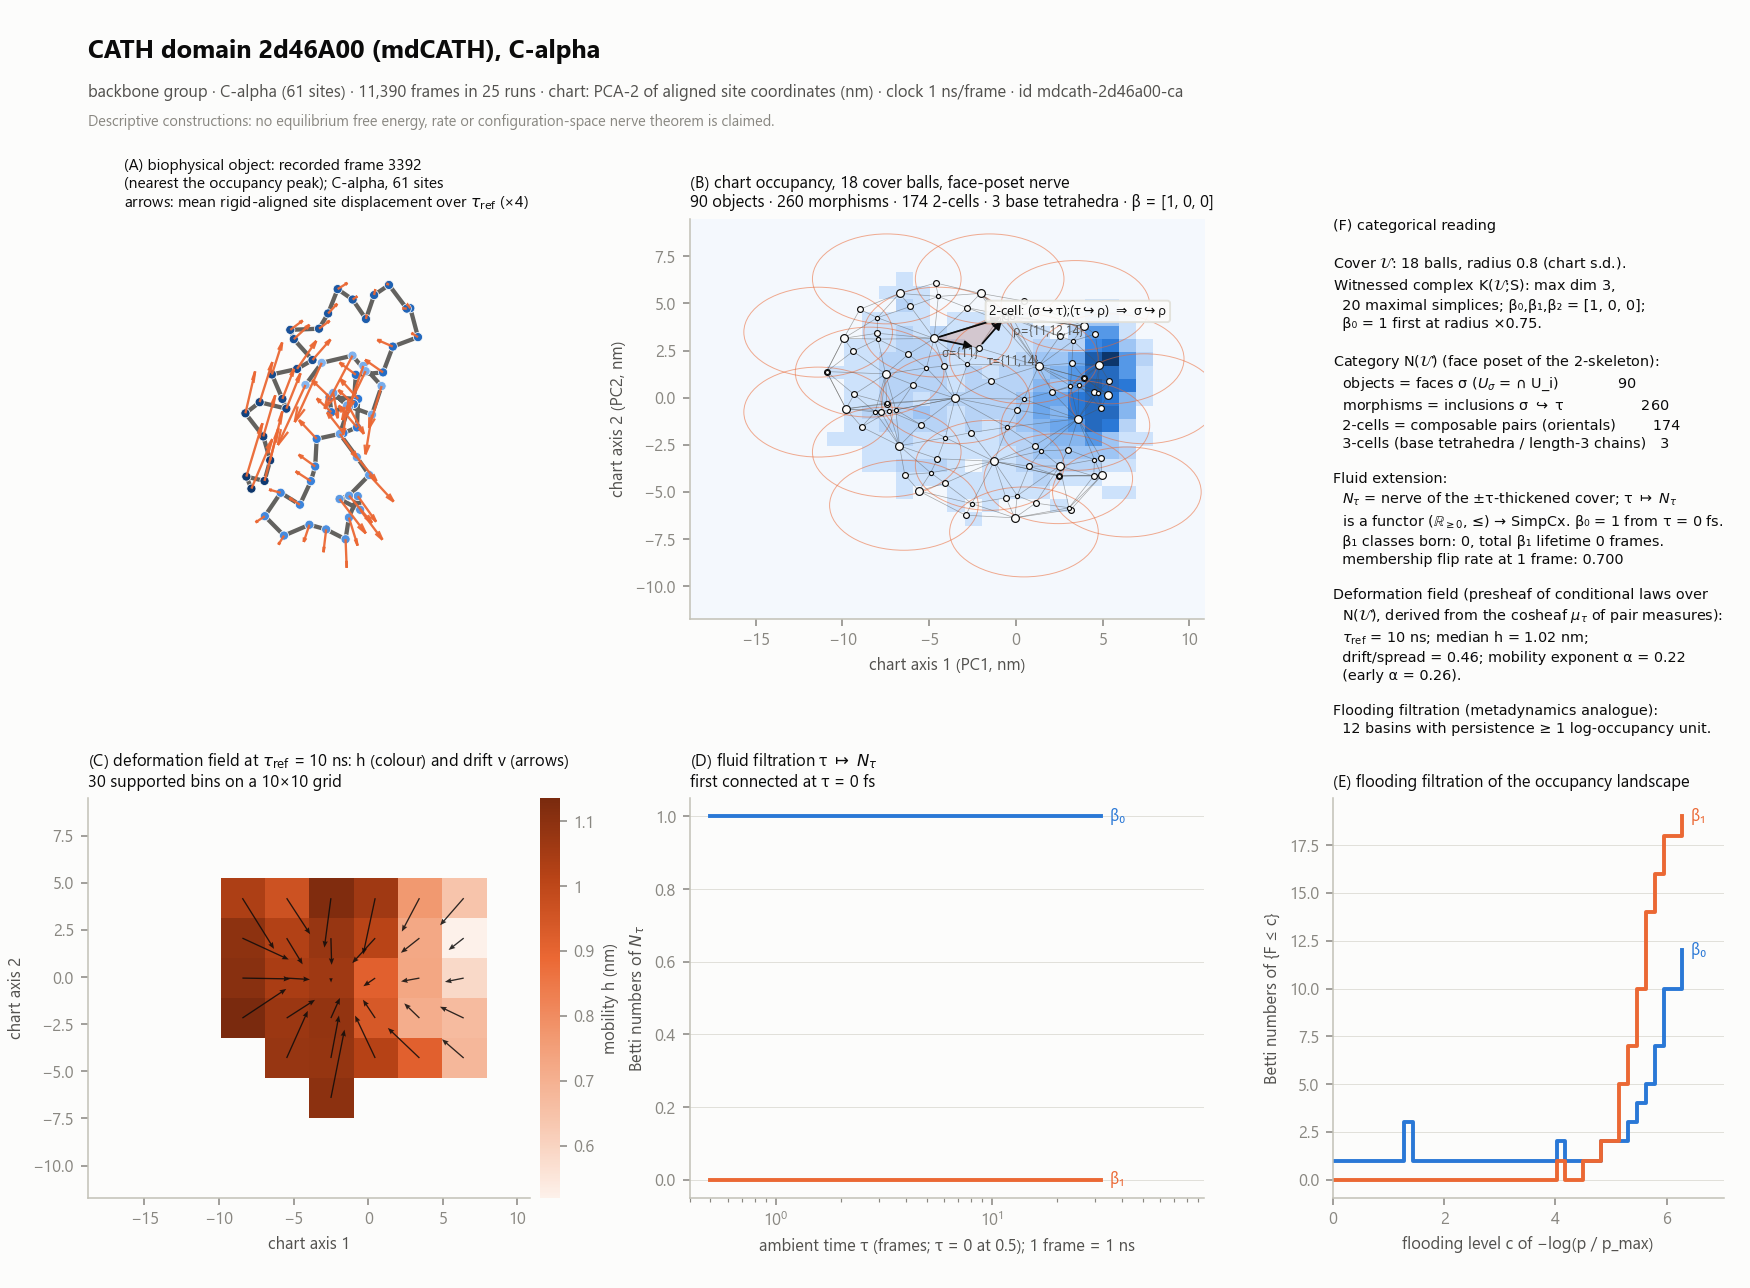
\includegraphics[width=\linewidth,height=.93\textheight,keepaspectratio]{systems/mdcath-2d46a00-ca/plate.png}\caption{CATH domain 2d46A00 (mdCATH), C-alpha (\texttt{mdcath-2d46a00-ca}). Source: https://huggingface.co/datasets/compsciencelab/mdCATH/resolve/main/data/mdcath\_dataset\_2d46A00.h5.}\end{figure}\clearpage
\begin{figure}[H]\centering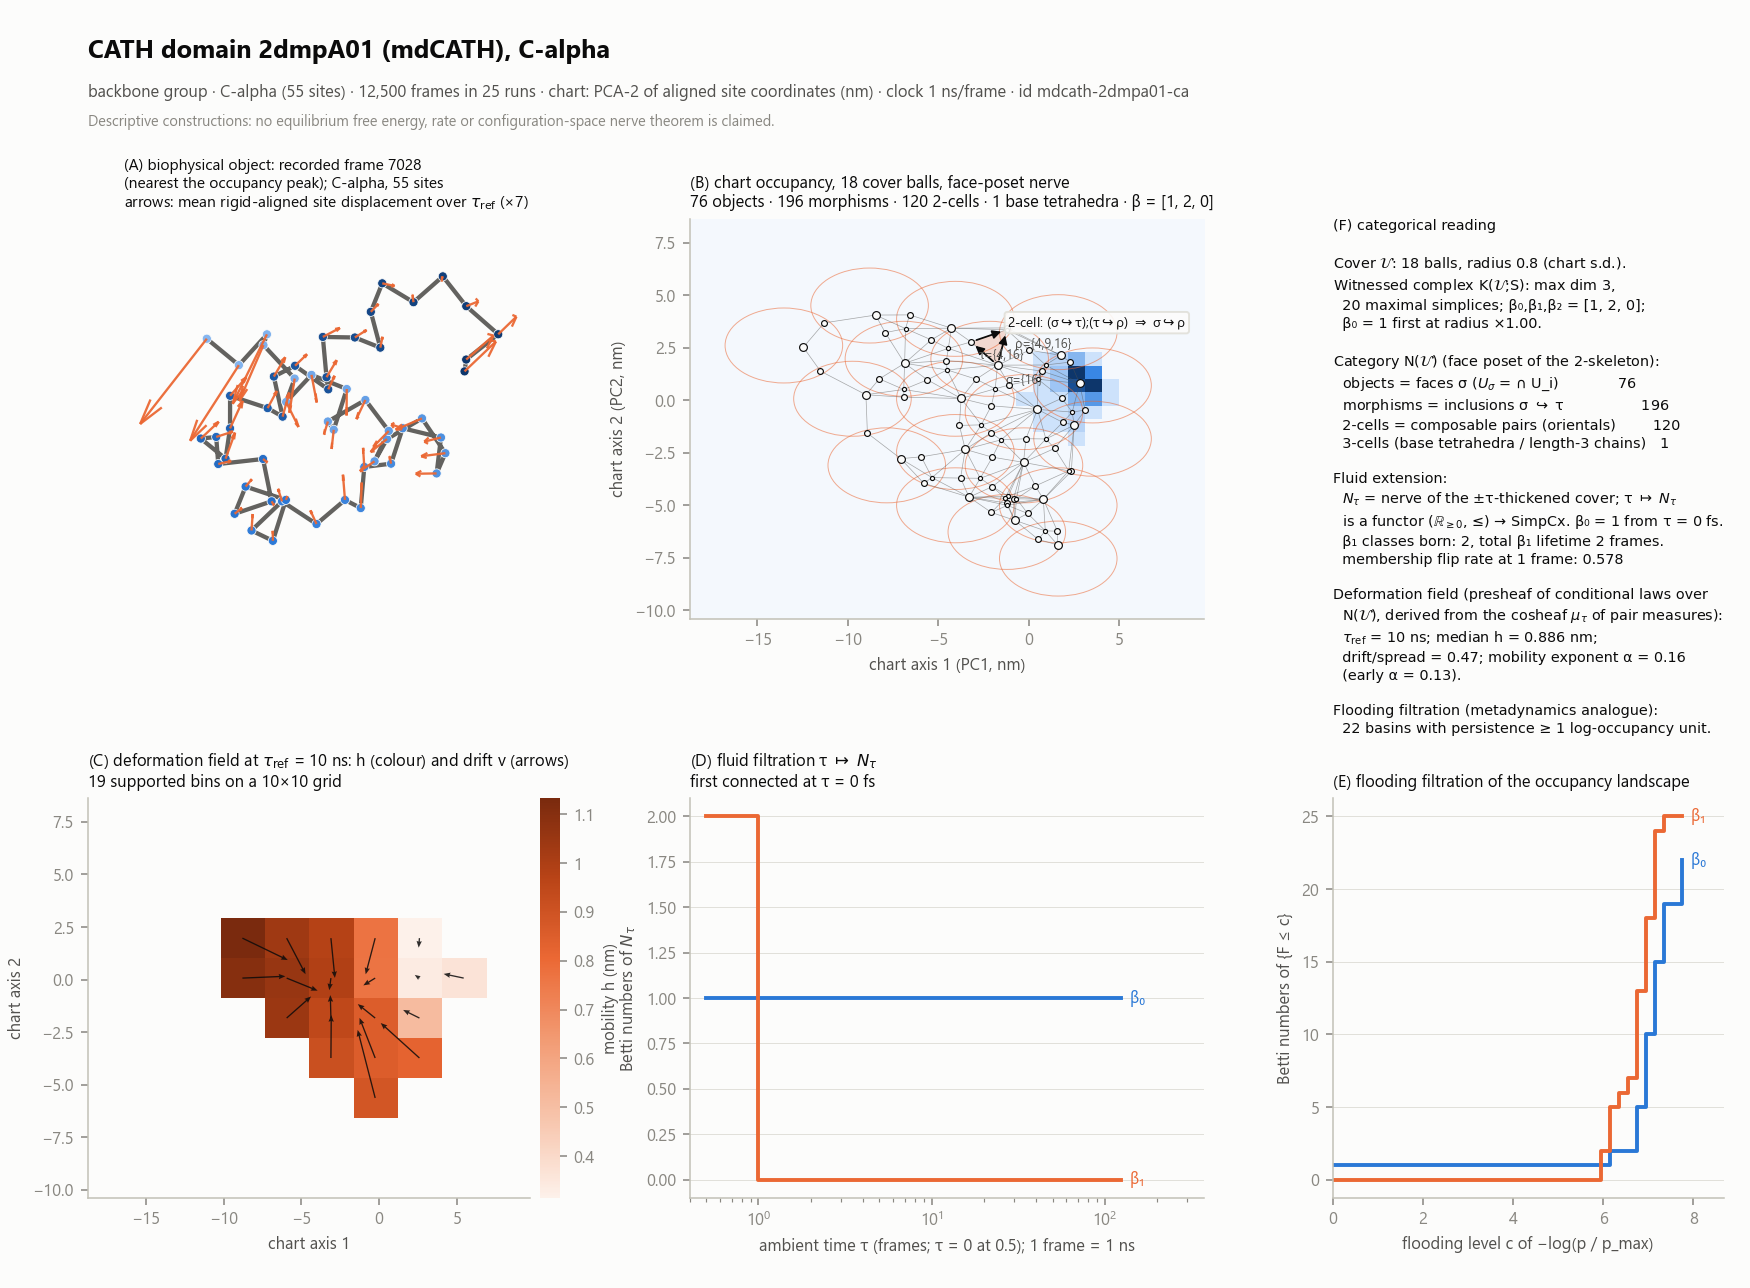
\includegraphics[width=\linewidth,height=.93\textheight,keepaspectratio]{systems/mdcath-2dmpa01-ca/plate.png}\caption{CATH domain 2dmpA01 (mdCATH), C-alpha (\texttt{mdcath-2dmpa01-ca}). Source: https://huggingface.co/datasets/compsciencelab/mdCATH/resolve/main/data/mdcath\_dataset\_2dmpA01.h5.}\end{figure}\clearpage
\begin{figure}[H]\centering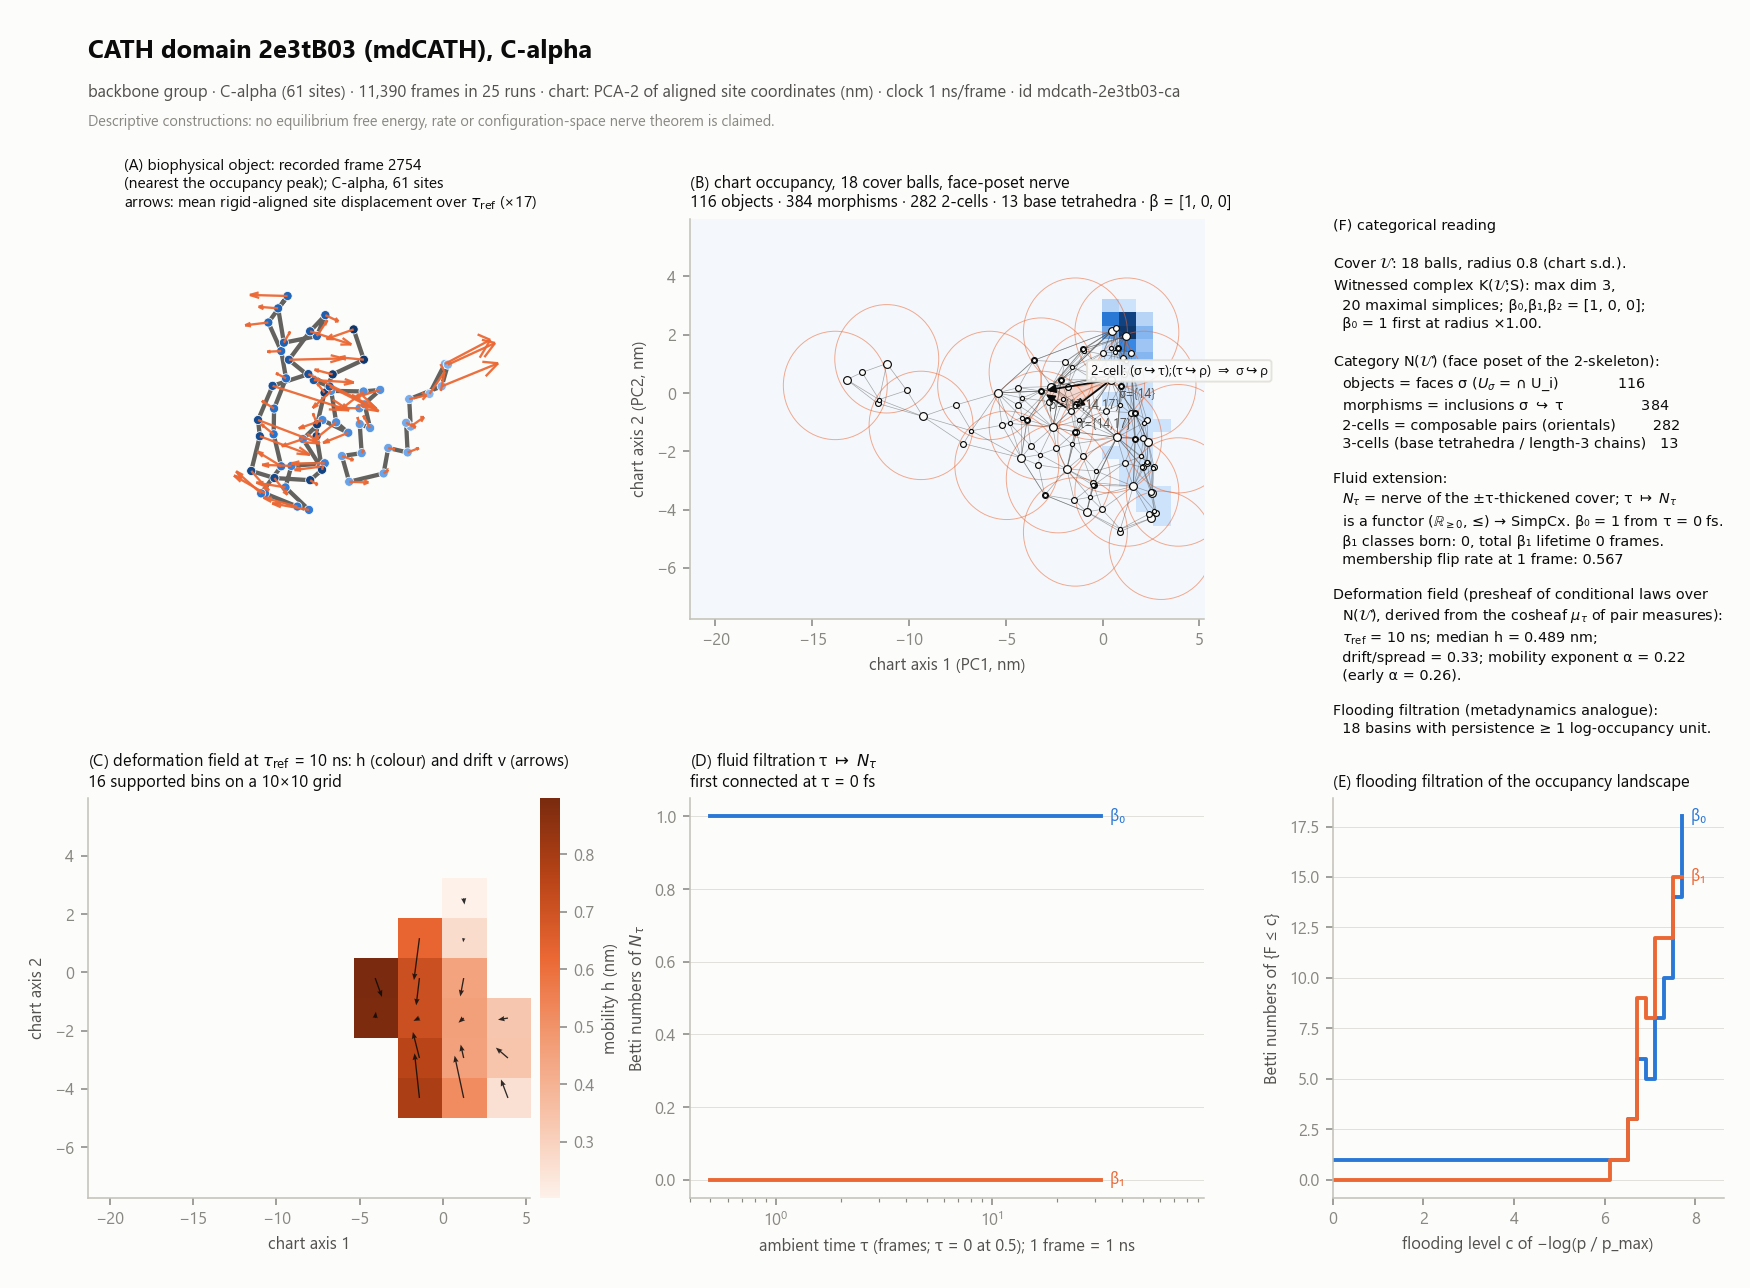
\includegraphics[width=\linewidth,height=.93\textheight,keepaspectratio]{systems/mdcath-2e3tb03-ca/plate.png}\caption{CATH domain 2e3tB03 (mdCATH), C-alpha (\texttt{mdcath-2e3tb03-ca}). Source: https://huggingface.co/datasets/compsciencelab/mdCATH/resolve/main/data/mdcath\_dataset\_2e3tB03.h5.}\end{figure}\clearpage
\begin{figure}[H]\centering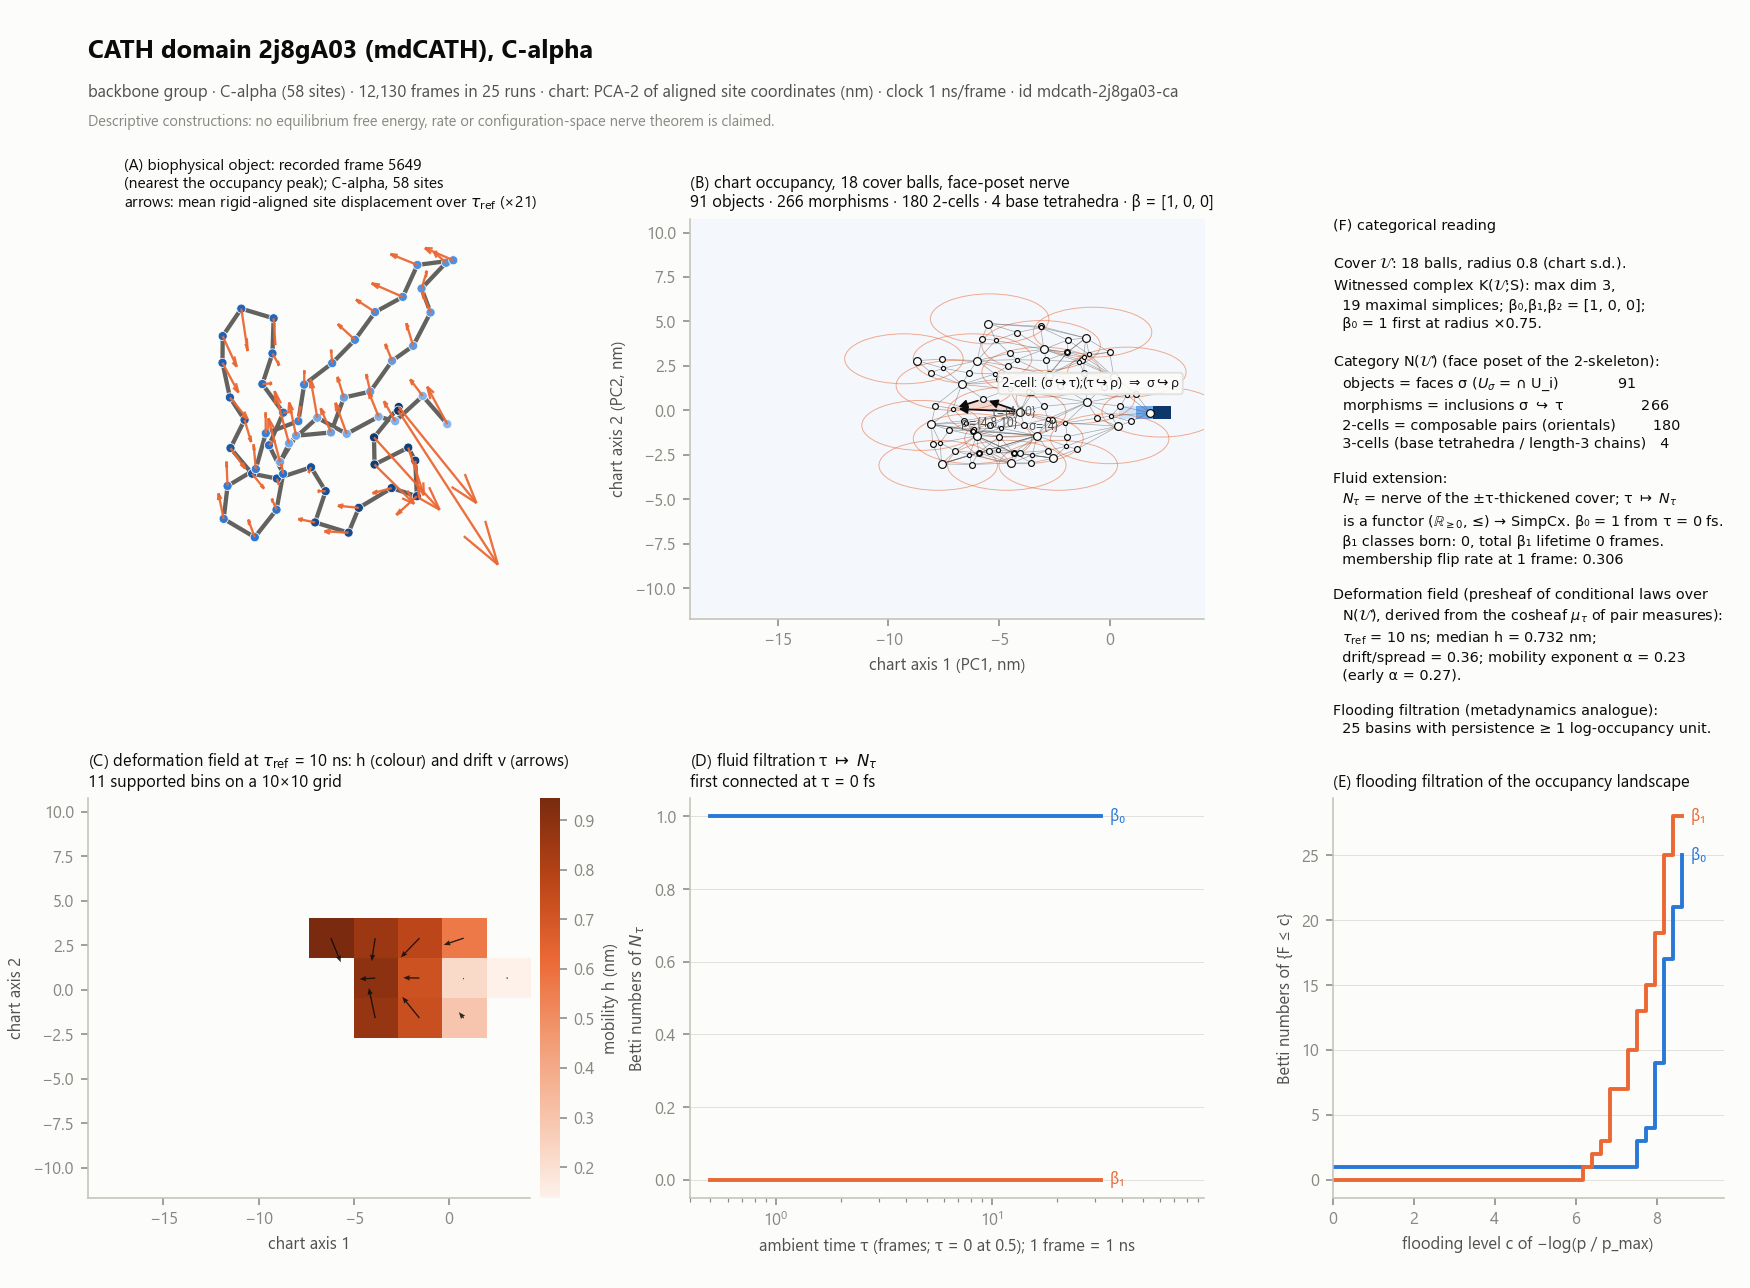
\includegraphics[width=\linewidth,height=.93\textheight,keepaspectratio]{systems/mdcath-2j8ga03-ca/plate.png}\caption{CATH domain 2j8gA03 (mdCATH), C-alpha (\texttt{mdcath-2j8ga03-ca}). Source: https://huggingface.co/datasets/compsciencelab/mdCATH/resolve/main/data/mdcath\_dataset\_2j8gA03.h5.}\end{figure}\clearpage
\begin{figure}[H]\centering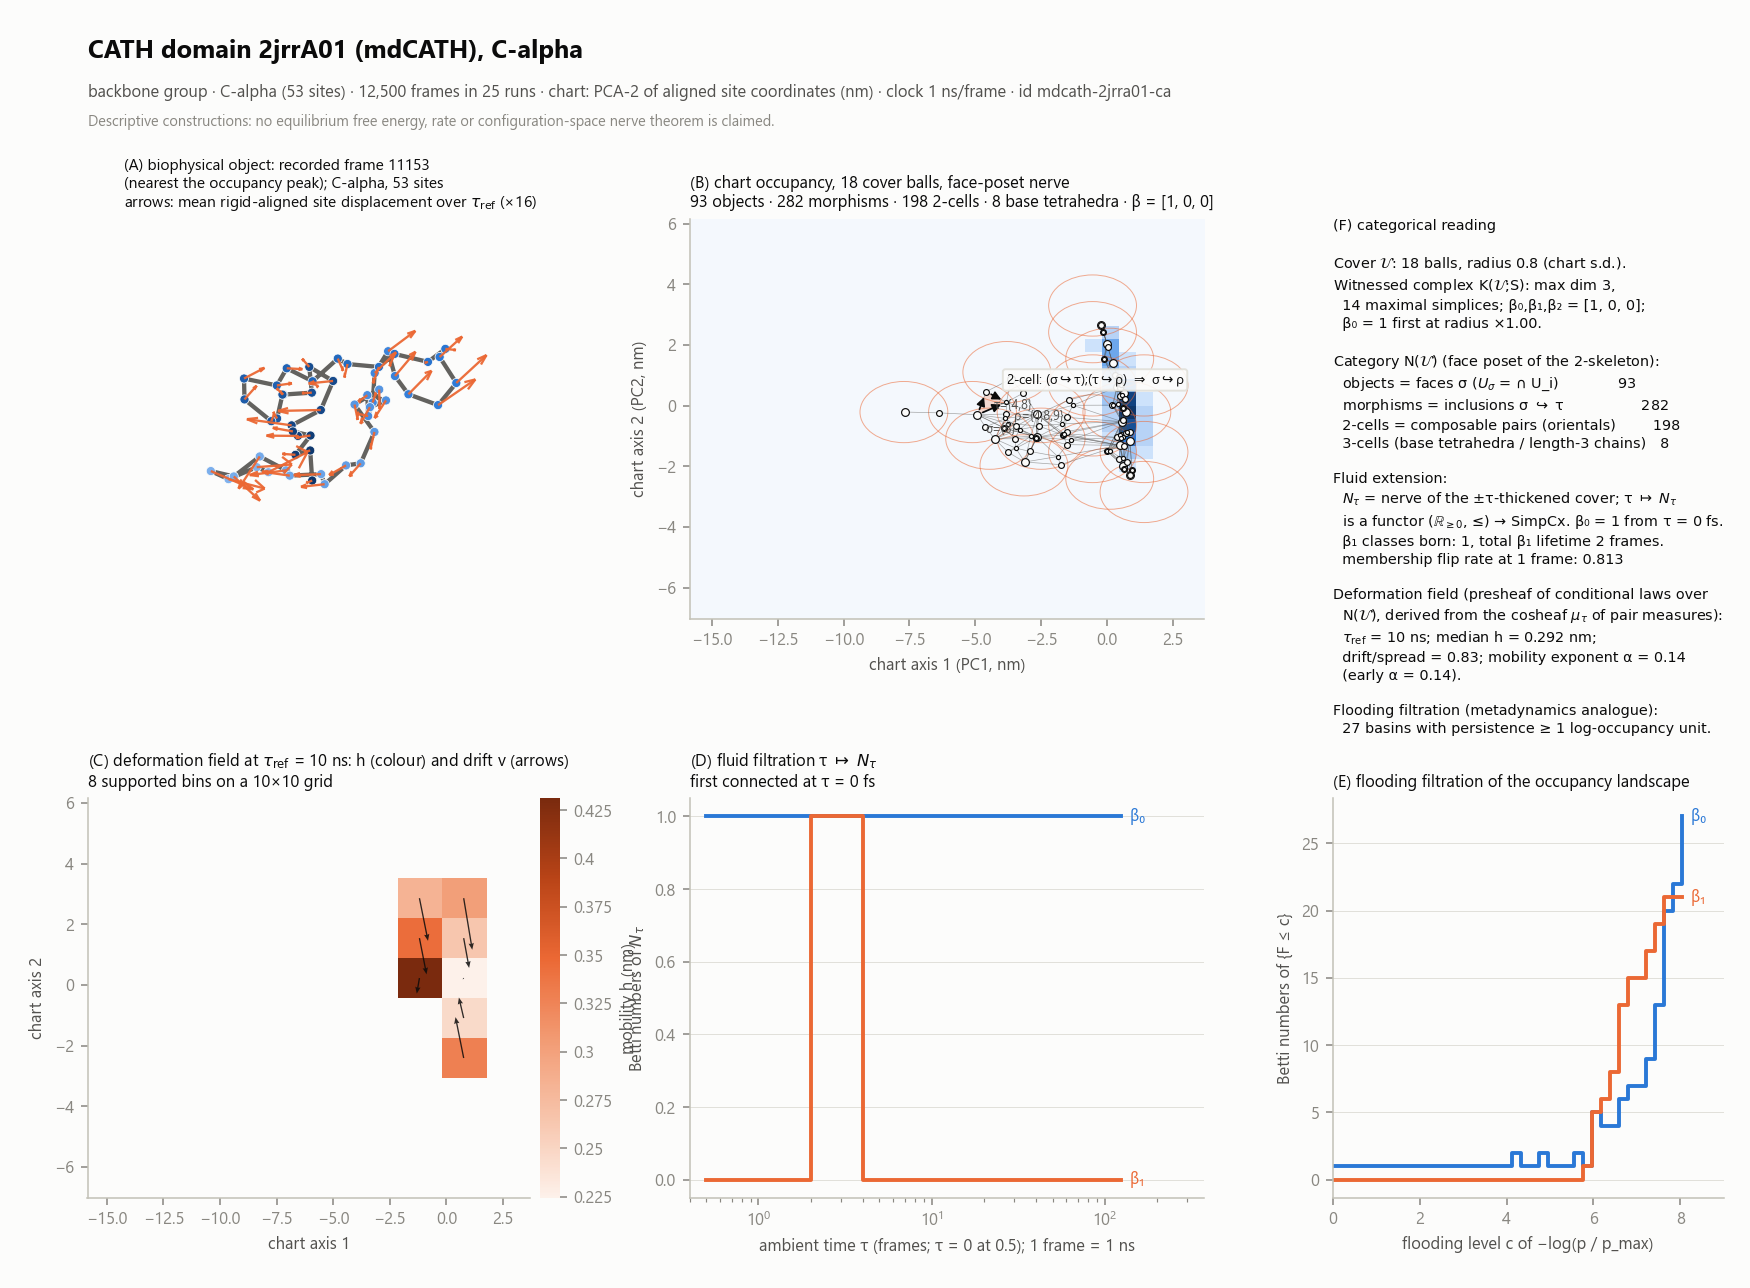
\includegraphics[width=\linewidth,height=.93\textheight,keepaspectratio]{systems/mdcath-2jrra01-ca/plate.png}\caption{CATH domain 2jrrA01 (mdCATH), C-alpha (\texttt{mdcath-2jrra01-ca}). Source: https://huggingface.co/datasets/compsciencelab/mdCATH/resolve/main/data/mdcath\_dataset\_2jrrA01.h5.}\end{figure}\clearpage
\begin{figure}[H]\centering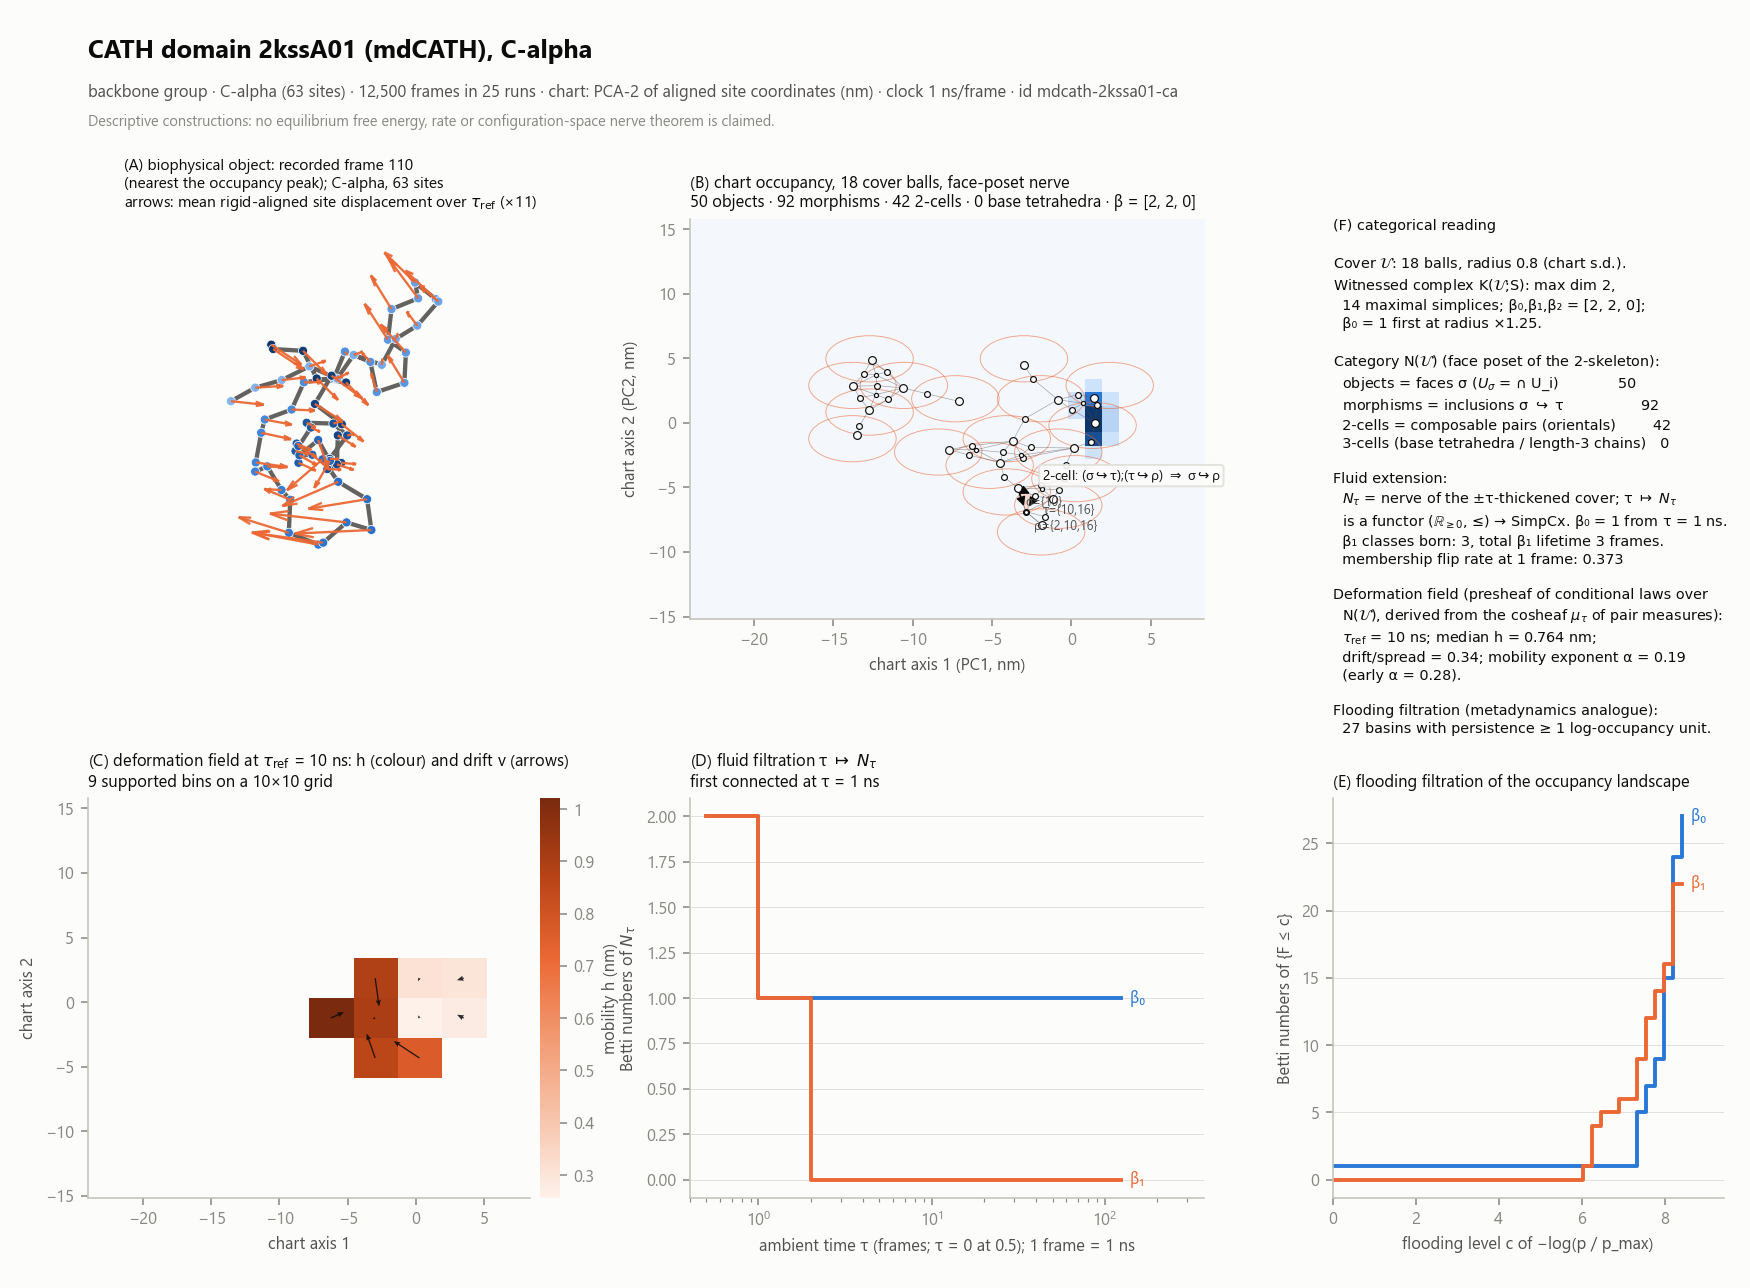
\includegraphics[width=\linewidth,height=.93\textheight,keepaspectratio]{systems/mdcath-2kssa01-ca/plate.png}\caption{CATH domain 2kssA01 (mdCATH), C-alpha (\texttt{mdcath-2kssa01-ca}). Source: https://huggingface.co/datasets/compsciencelab/mdCATH/resolve/main/data/mdcath\_dataset\_2kssA01.h5.}\end{figure}\clearpage
\begin{figure}[H]\centering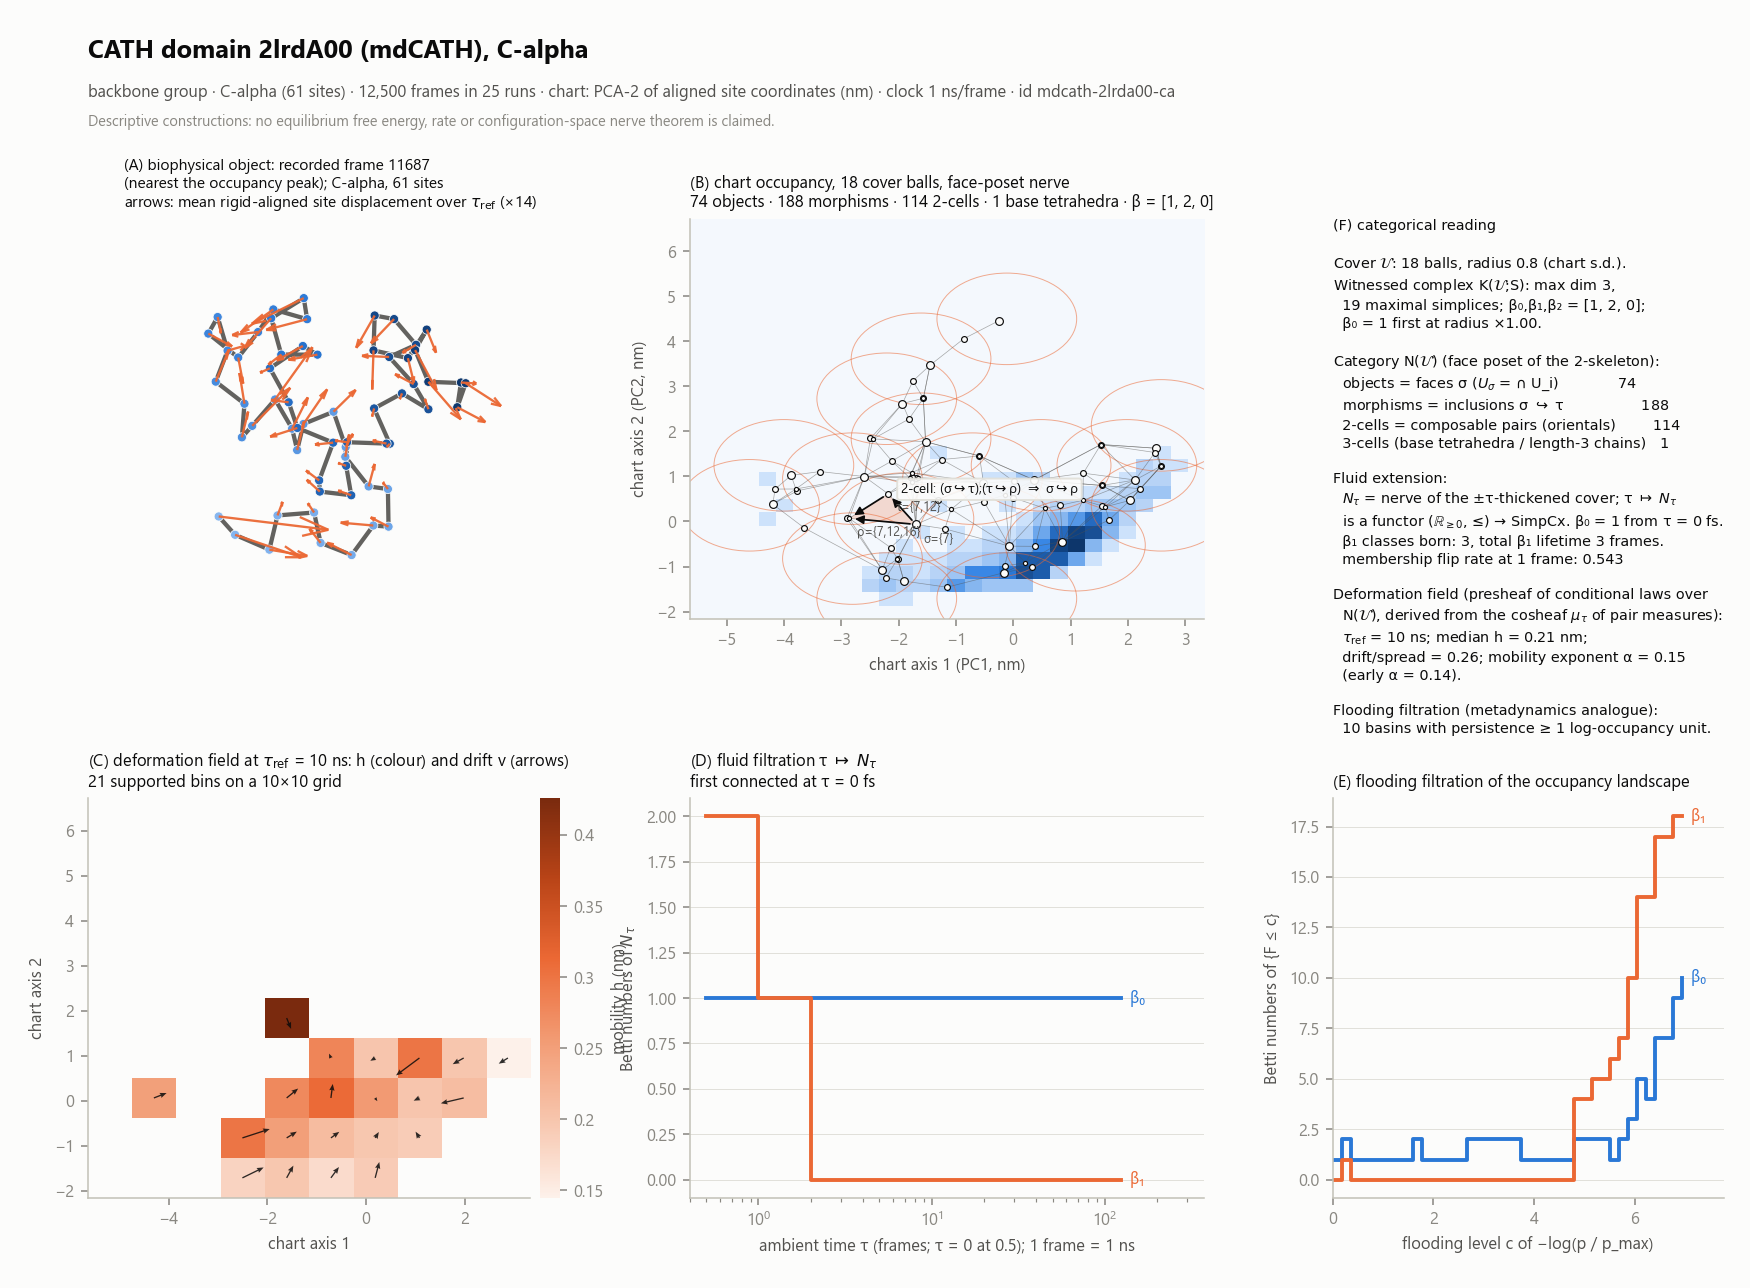
\includegraphics[width=\linewidth,height=.93\textheight,keepaspectratio]{systems/mdcath-2lrda00-ca/plate.png}\caption{CATH domain 2lrdA00 (mdCATH), C-alpha (\texttt{mdcath-2lrda00-ca}). Source: https://huggingface.co/datasets/compsciencelab/mdCATH/resolve/main/data/mdcath\_dataset\_2lrdA00.h5.}\end{figure}\clearpage
\begin{figure}[H]\centering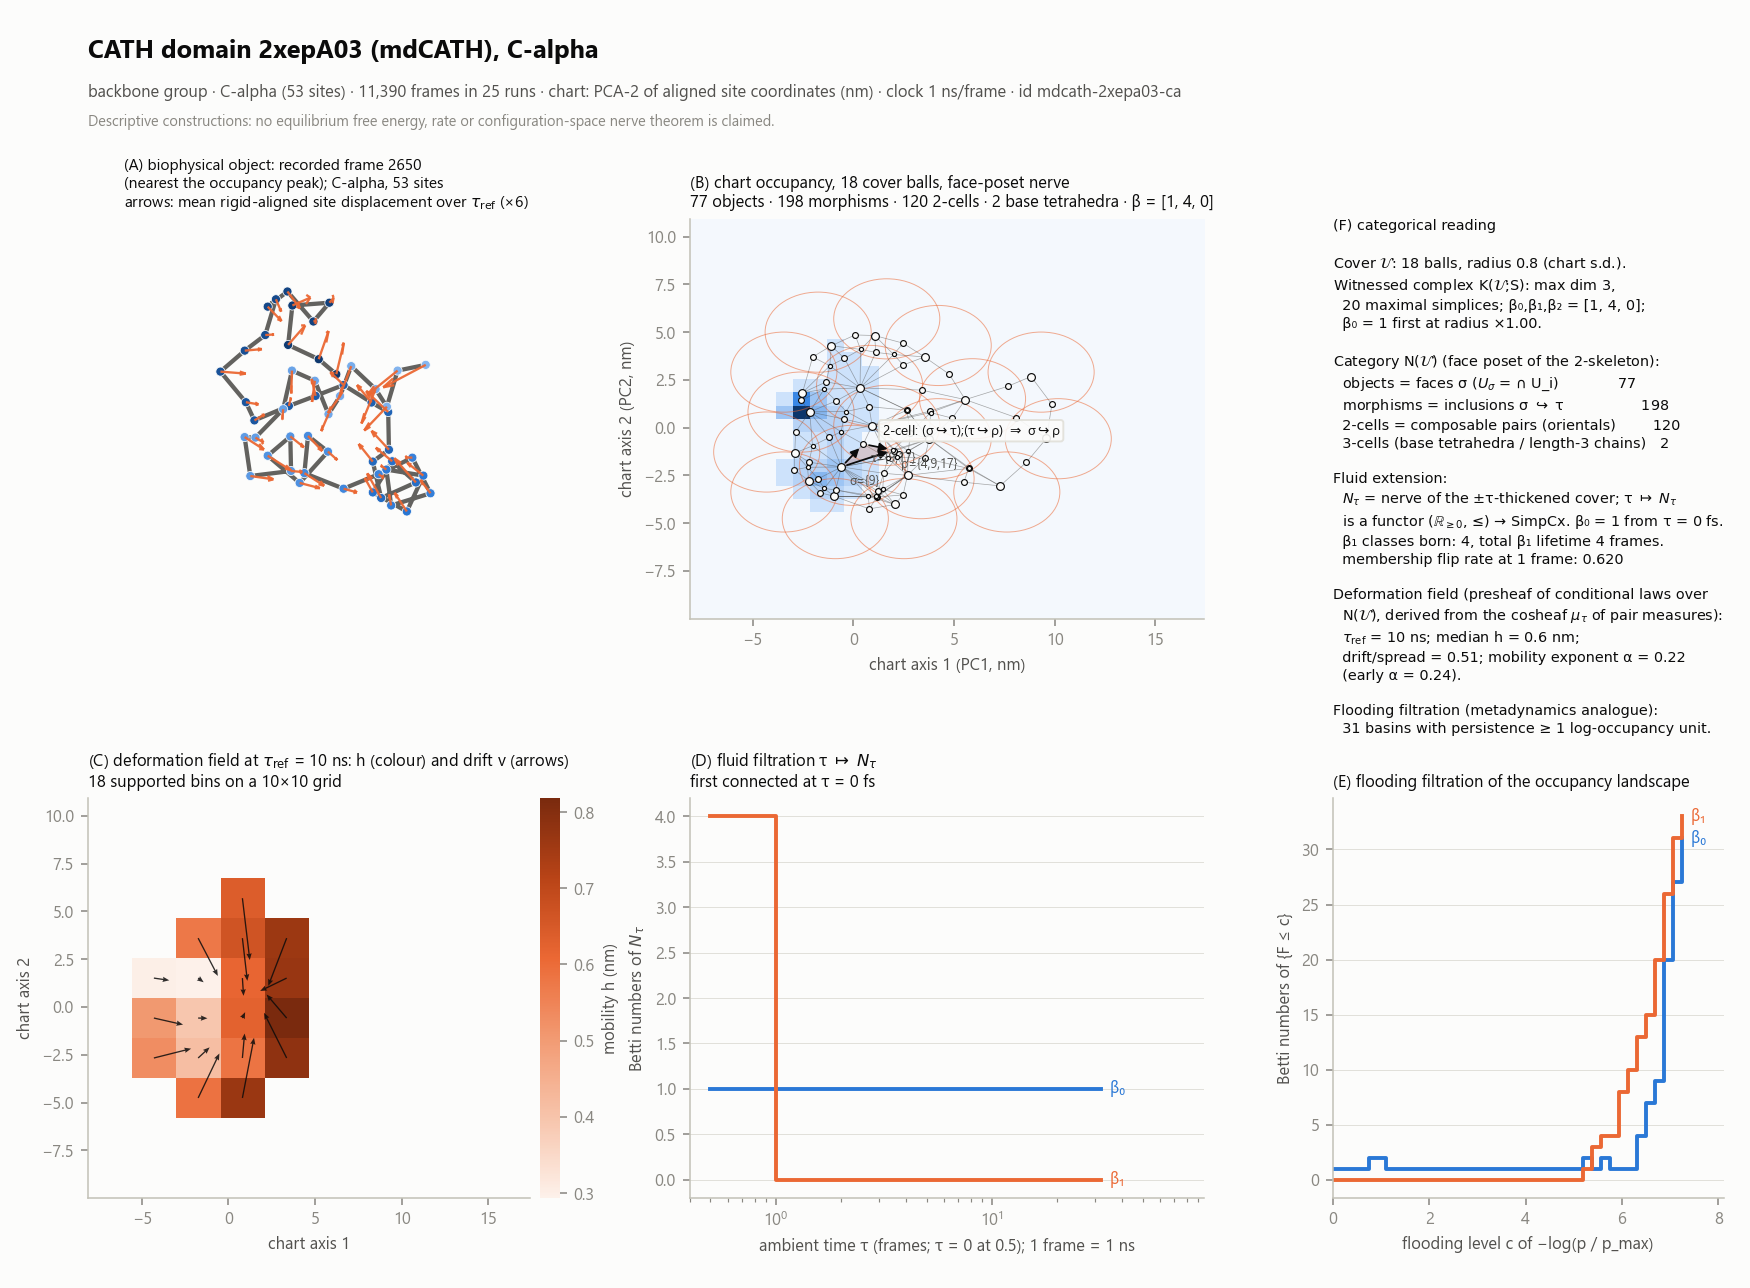
\includegraphics[width=\linewidth,height=.93\textheight,keepaspectratio]{systems/mdcath-2xepa03-ca/plate.png}\caption{CATH domain 2xepA03 (mdCATH), C-alpha (\texttt{mdcath-2xepa03-ca}). Source: https://huggingface.co/datasets/compsciencelab/mdCATH/resolve/main/data/mdcath\_dataset\_2xepA03.h5.}\end{figure}\clearpage
\begin{figure}[H]\centering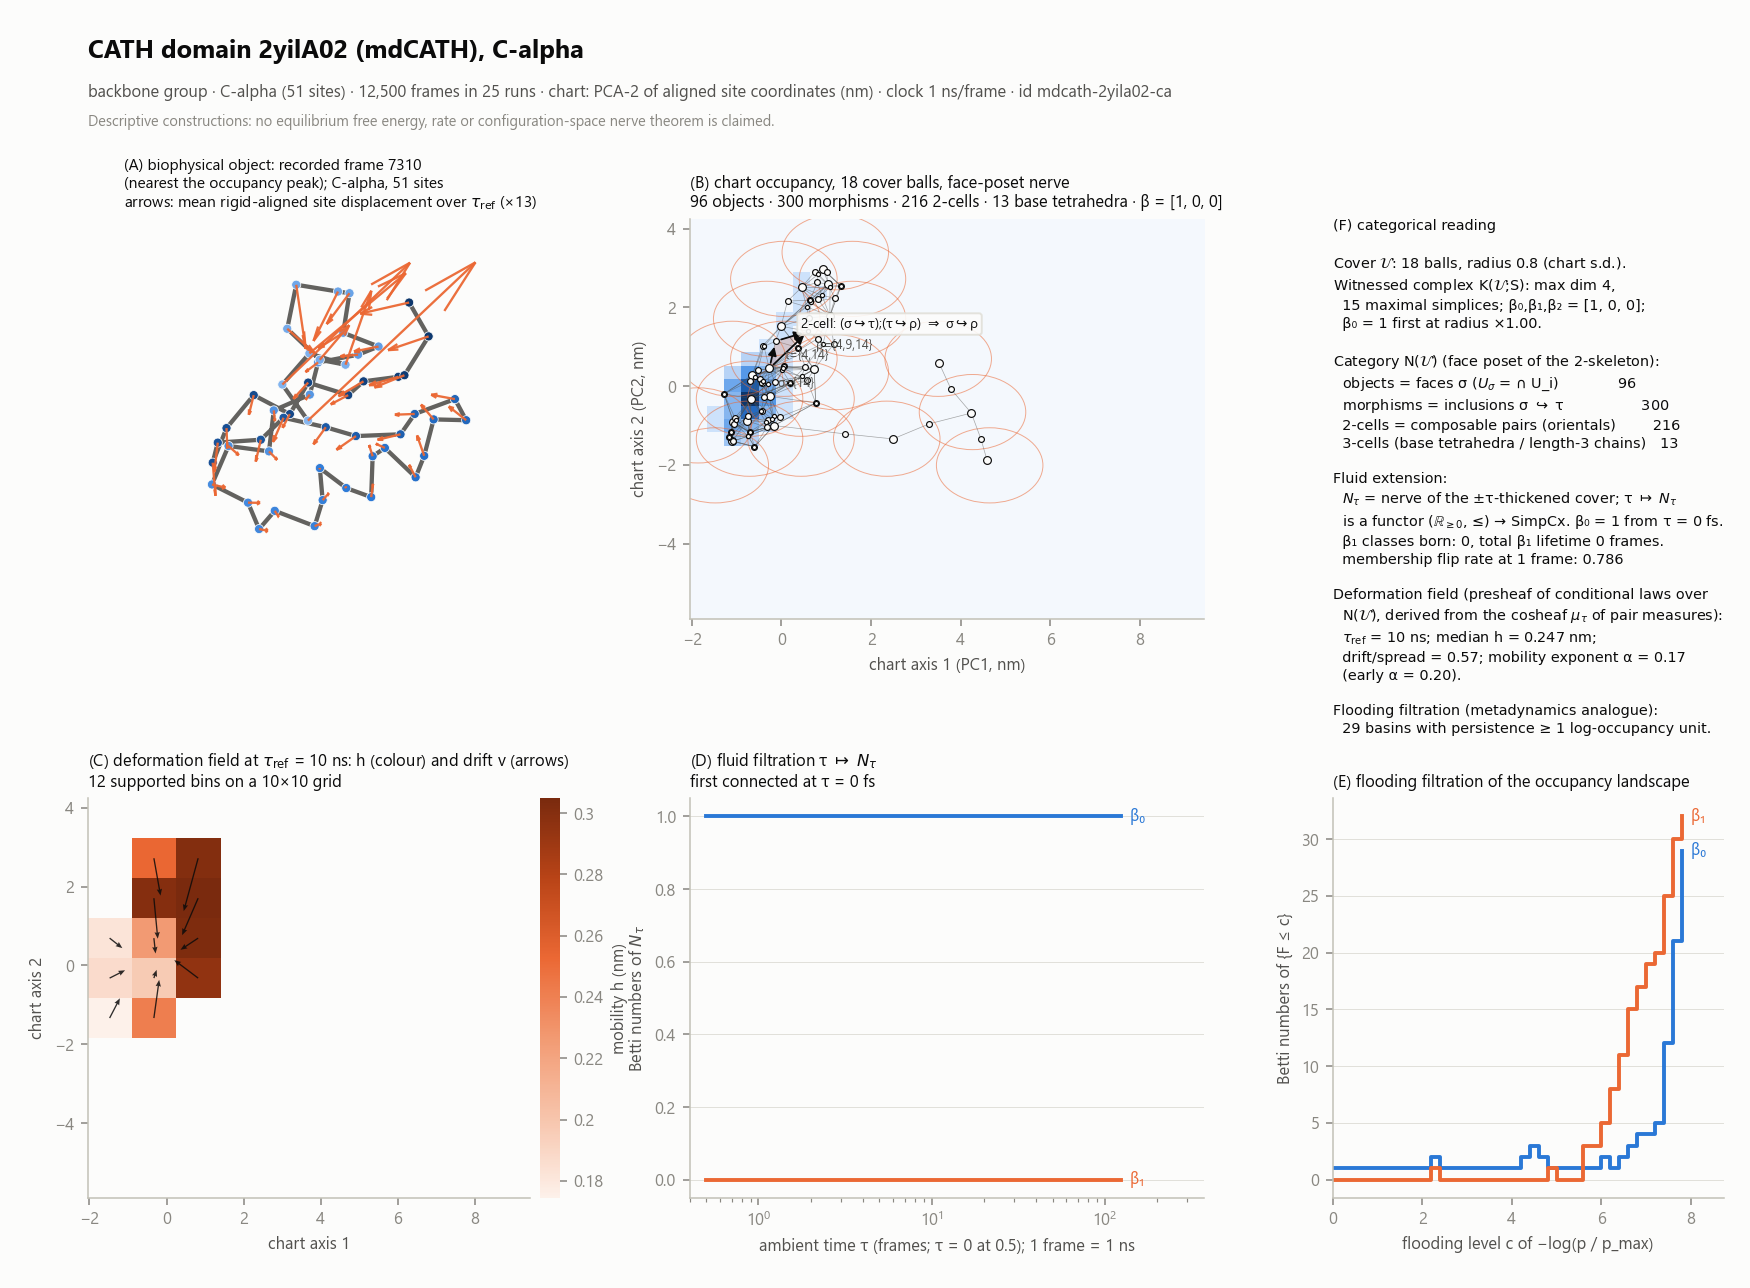
\includegraphics[width=\linewidth,height=.93\textheight,keepaspectratio]{systems/mdcath-2yila02-ca/plate.png}\caption{CATH domain 2yilA02 (mdCATH), C-alpha (\texttt{mdcath-2yila02-ca}). Source: https://huggingface.co/datasets/compsciencelab/mdCATH/resolve/main/data/mdcath\_dataset\_2yilA02.h5.}\end{figure}\clearpage
\begin{figure}[H]\centering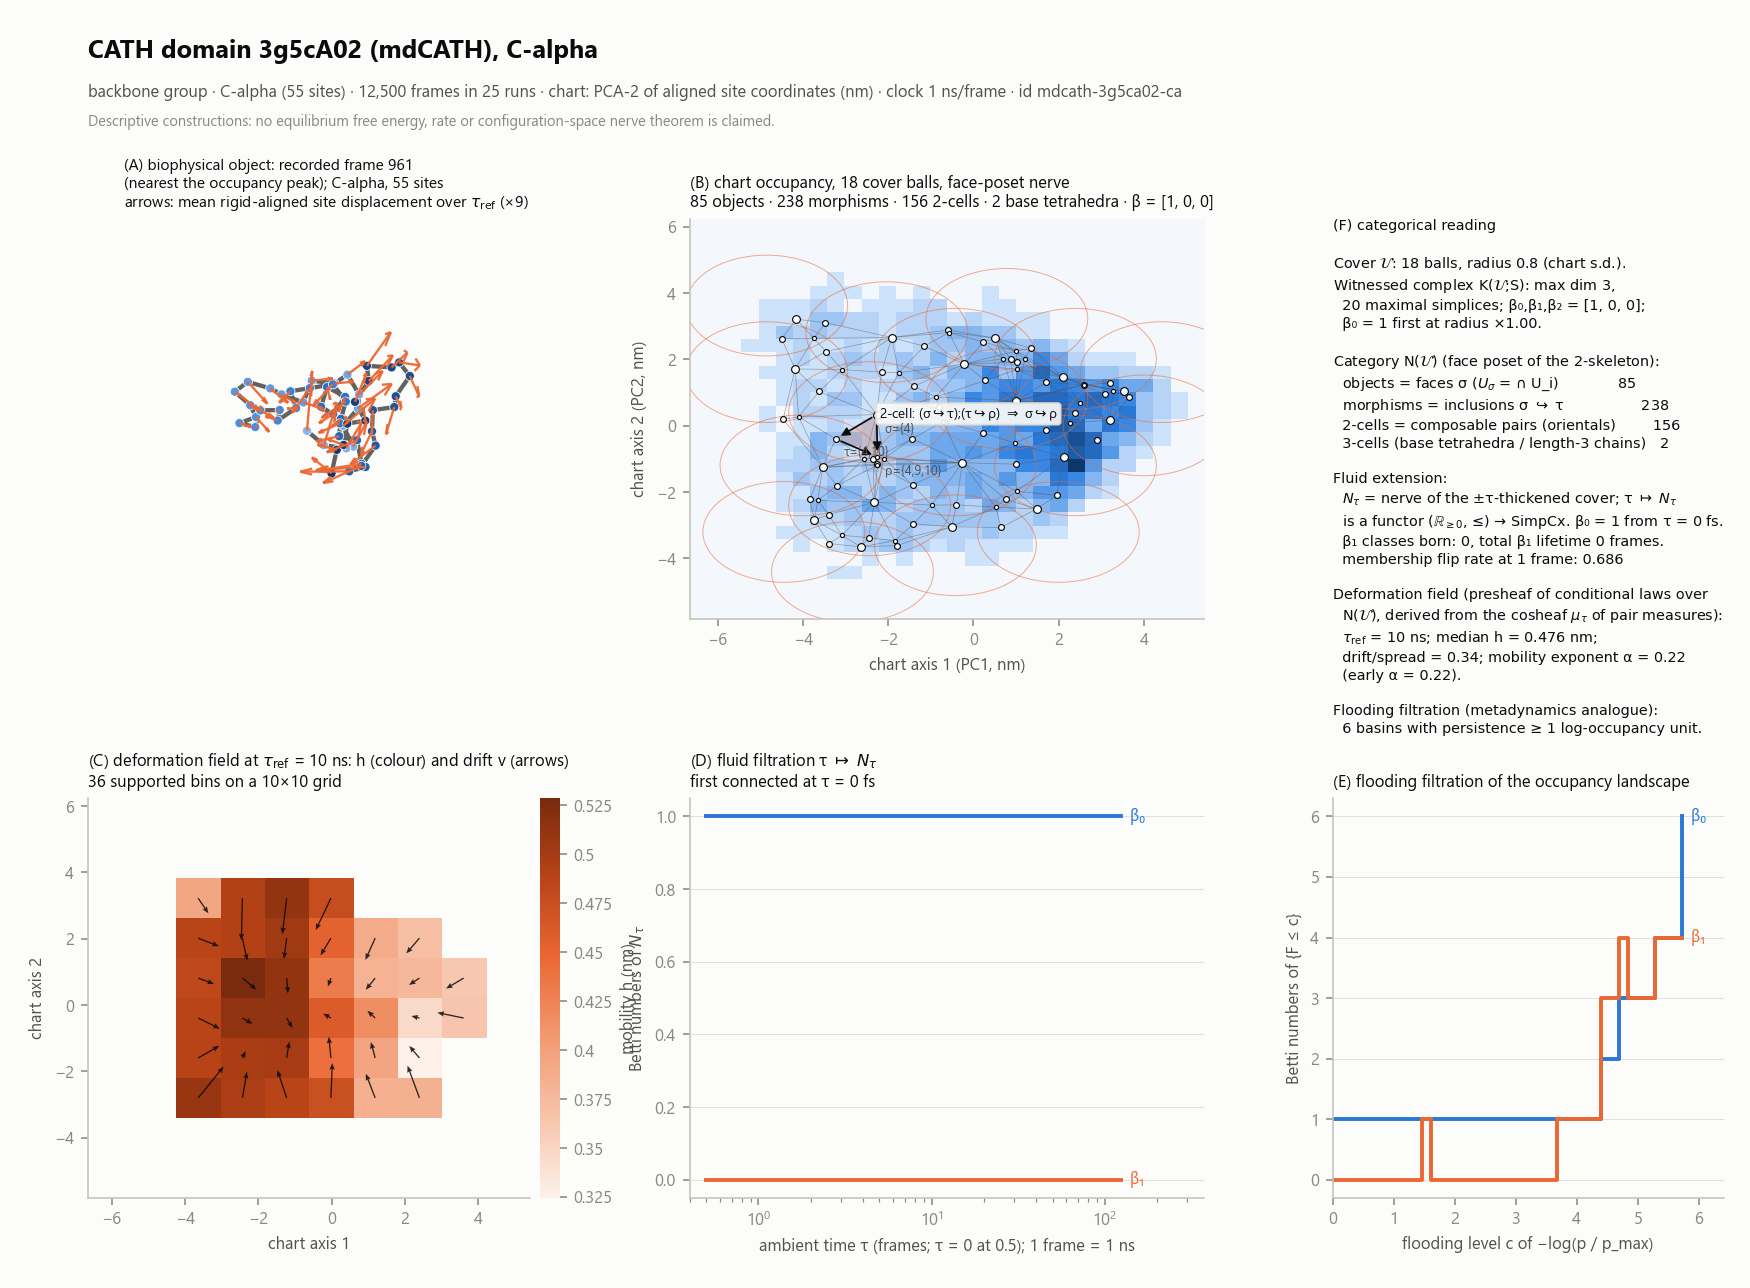
\includegraphics[width=\linewidth,height=.93\textheight,keepaspectratio]{systems/mdcath-3g5ca02-ca/plate.png}\caption{CATH domain 3g5cA02 (mdCATH), C-alpha (\texttt{mdcath-3g5ca02-ca}). Source: https://huggingface.co/datasets/compsciencelab/mdCATH/resolve/main/data/mdcath\_dataset\_3g5cA02.h5.}\end{figure}\clearpage
\begin{figure}[H]\centering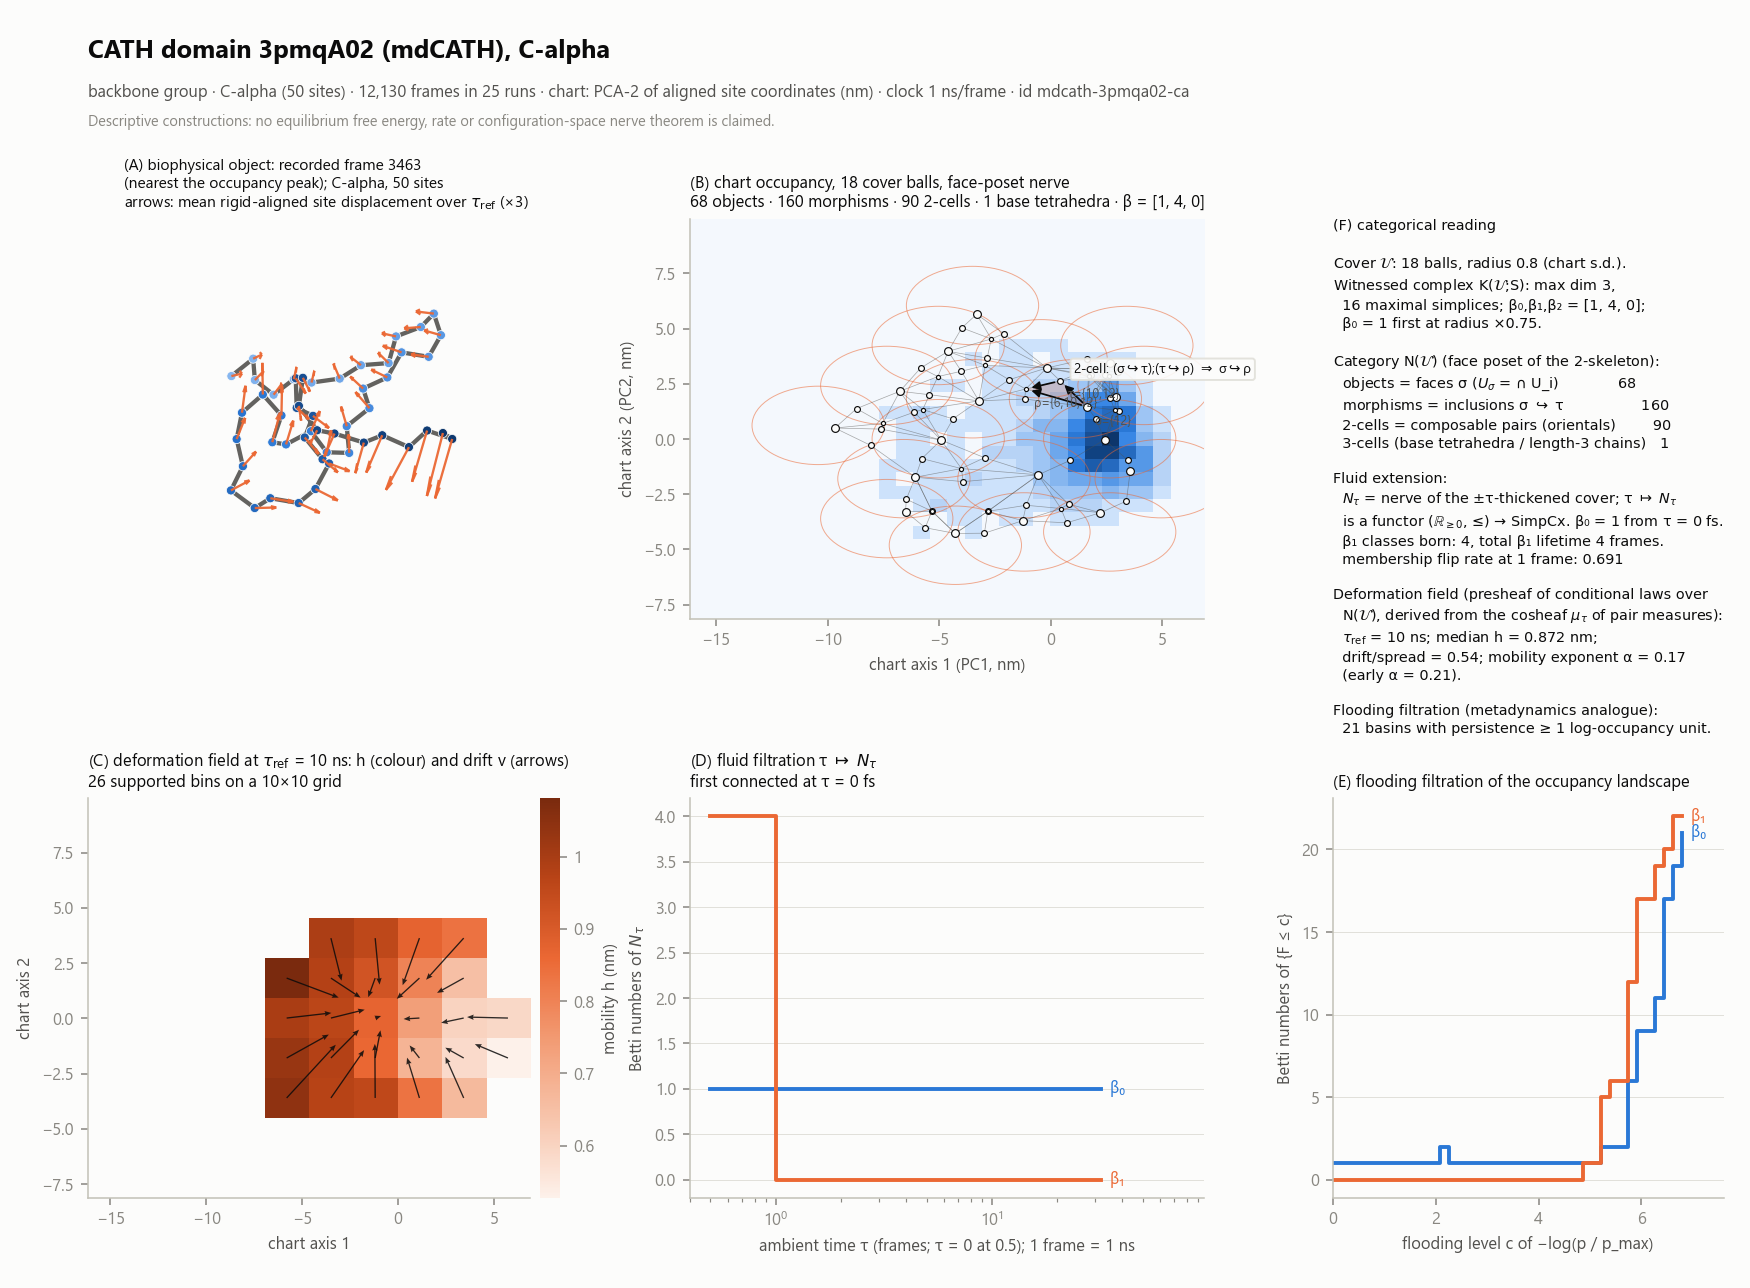
\includegraphics[width=\linewidth,height=.93\textheight,keepaspectratio]{systems/mdcath-3pmqa02-ca/plate.png}\caption{CATH domain 3pmqA02 (mdCATH), C-alpha (\texttt{mdcath-3pmqa02-ca}). Source: https://huggingface.co/datasets/compsciencelab/mdCATH/resolve/main/data/mdcath\_dataset\_3pmqA02.h5.}\end{figure}\clearpage
\begin{figure}[H]\centering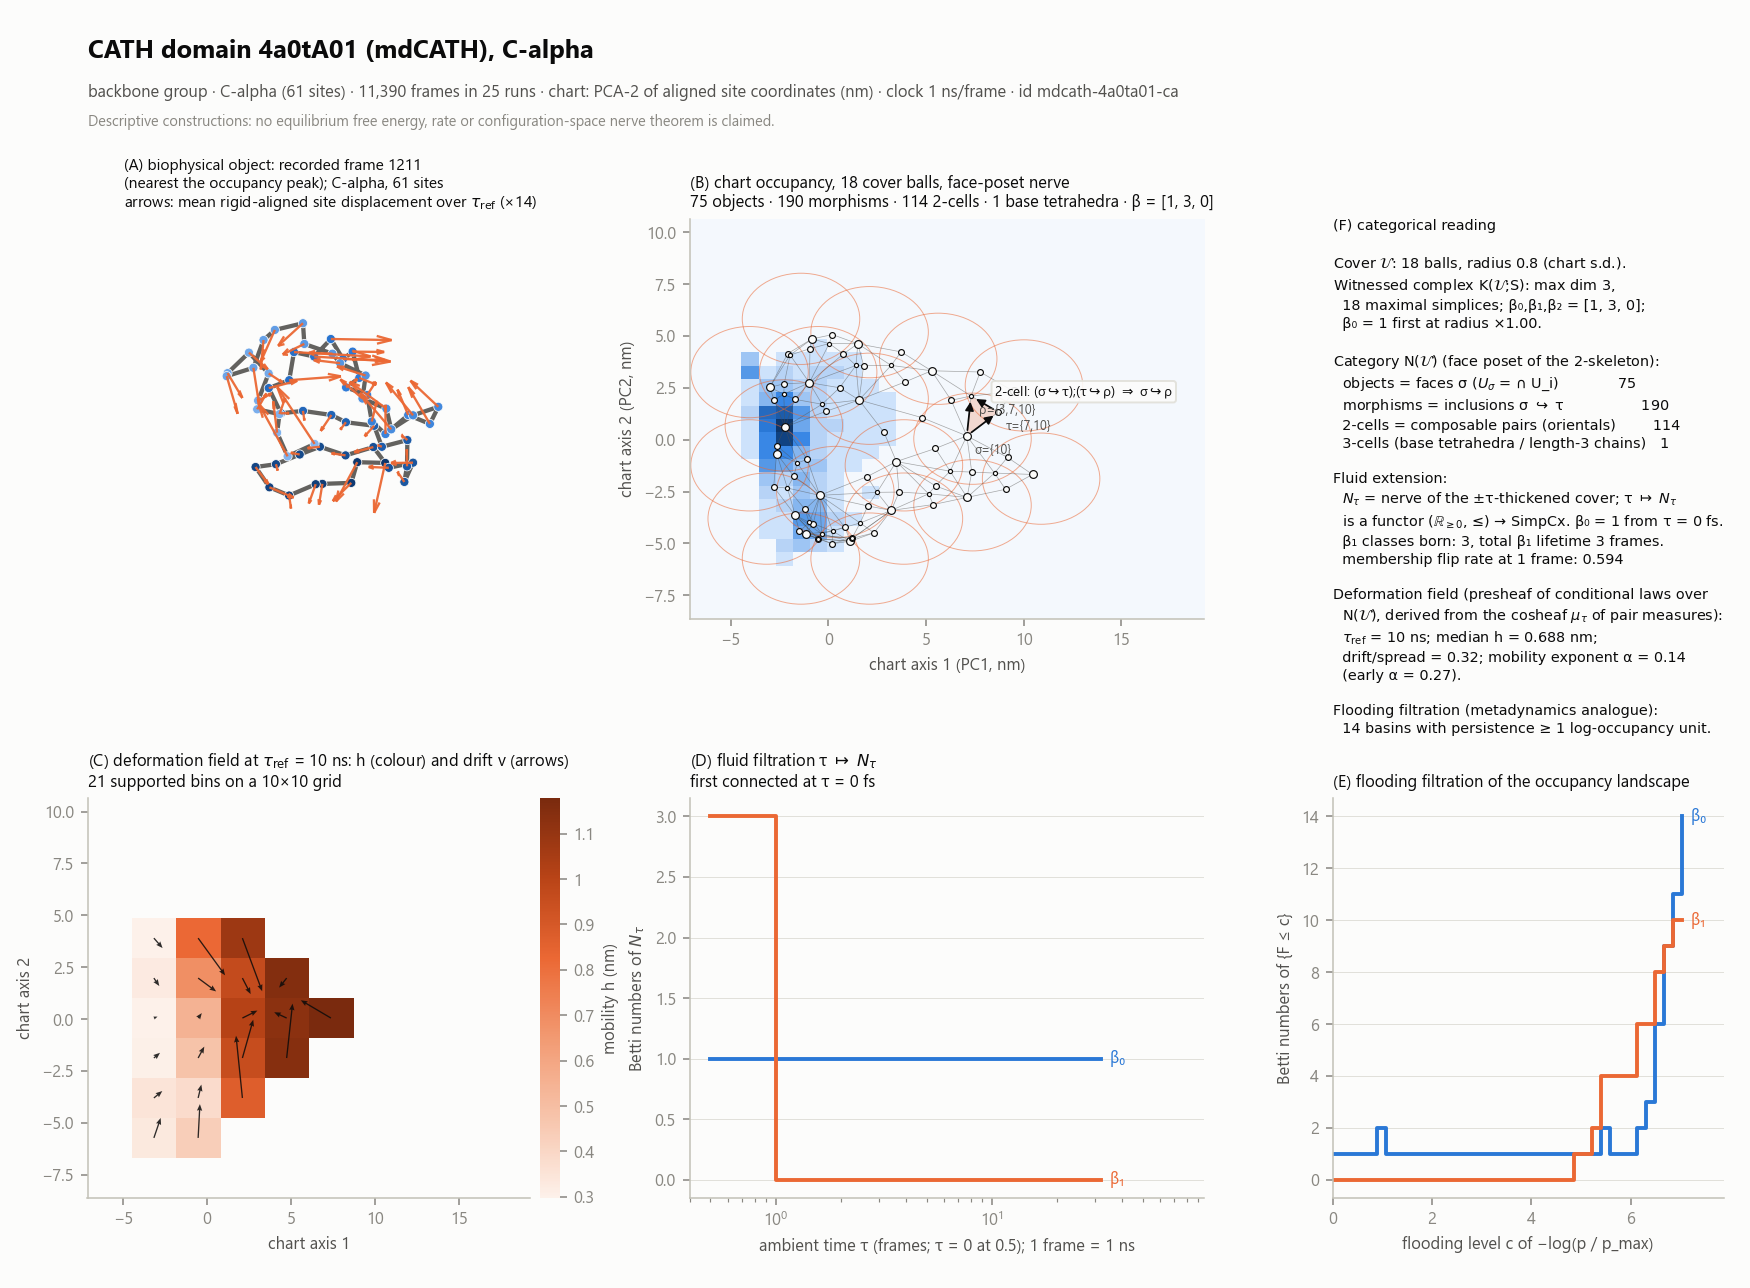
\includegraphics[width=\linewidth,height=.93\textheight,keepaspectratio]{systems/mdcath-4a0ta01-ca/plate.png}\caption{CATH domain 4a0tA01 (mdCATH), C-alpha (\texttt{mdcath-4a0ta01-ca}). Source: https://huggingface.co/datasets/compsciencelab/mdCATH/resolve/main/data/mdcath\_dataset\_4a0tA01.h5.}\end{figure}\clearpage
\begin{figure}[H]\centering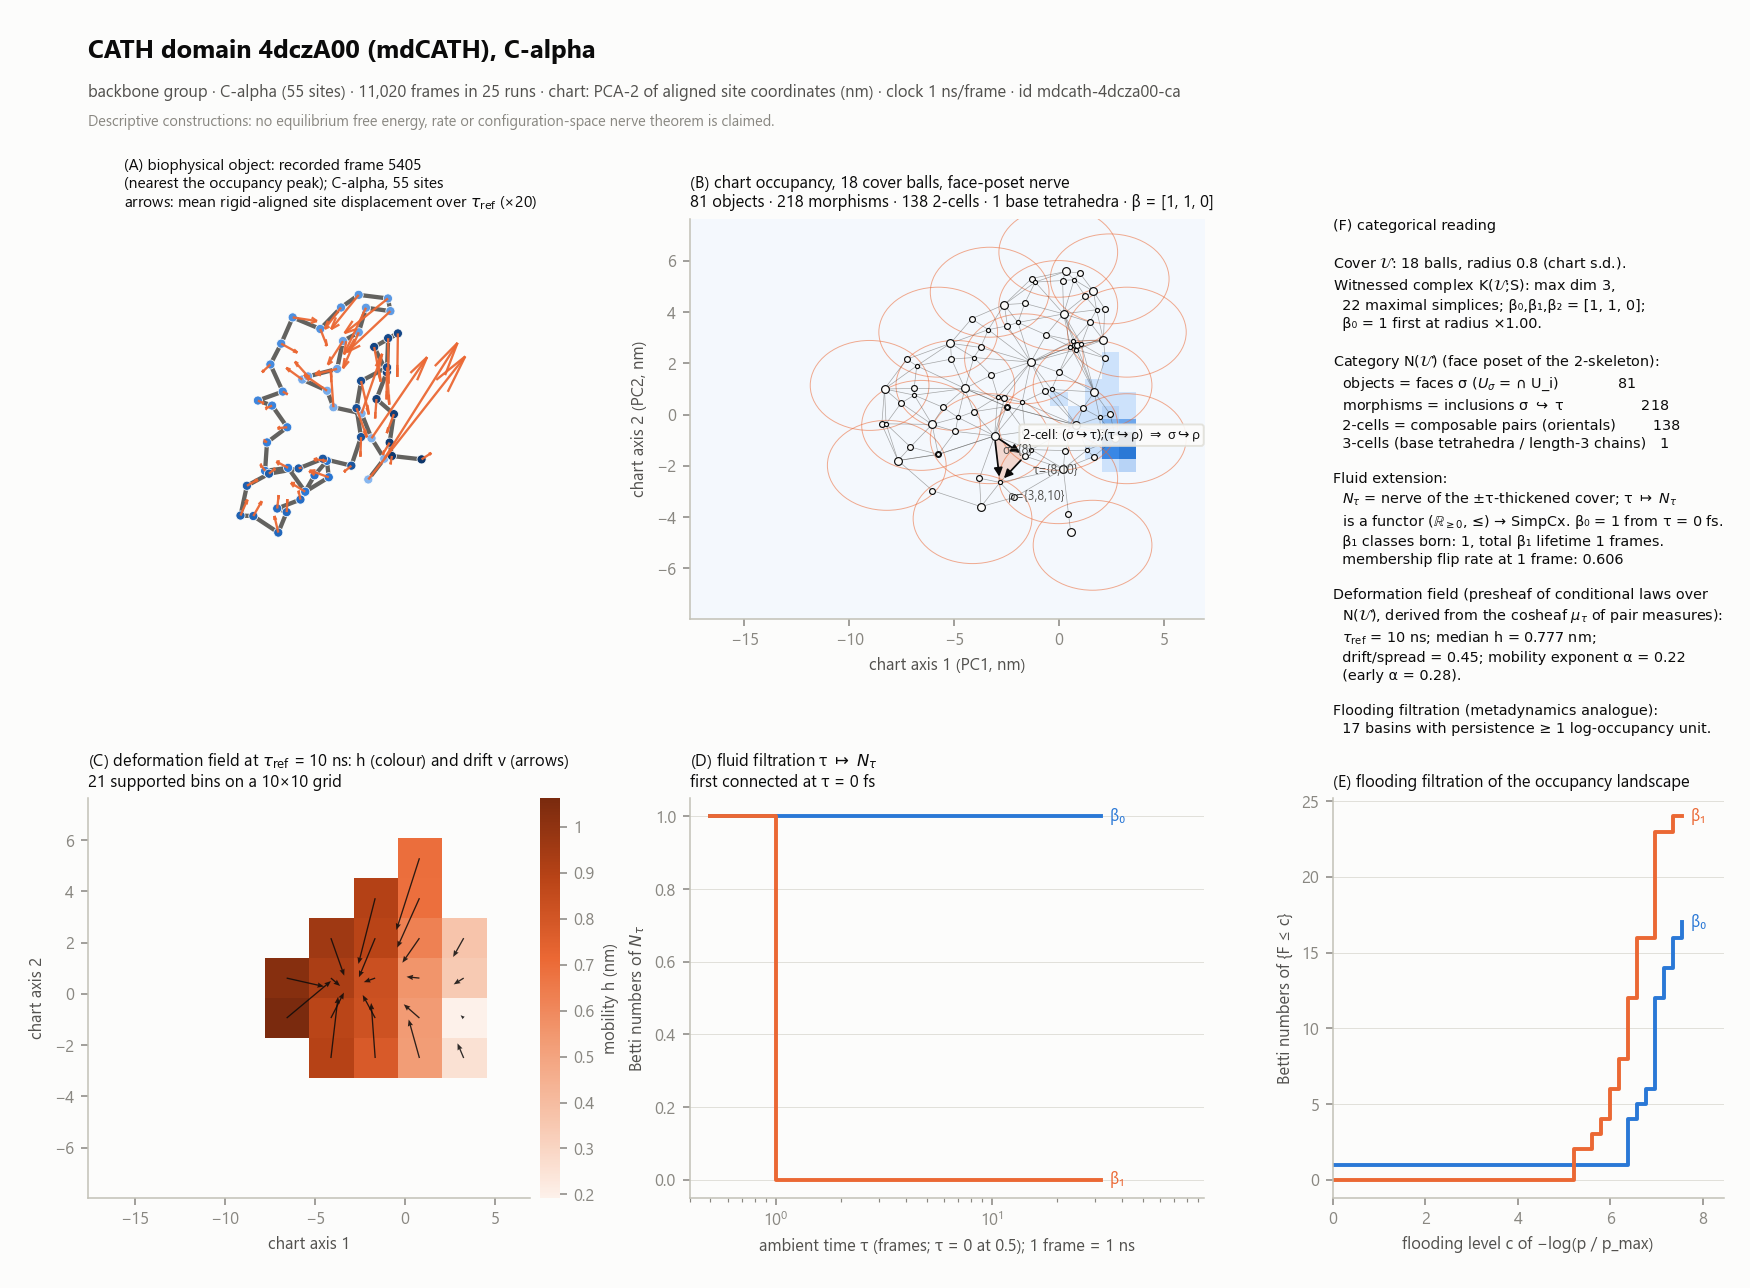
\includegraphics[width=\linewidth,height=.93\textheight,keepaspectratio]{systems/mdcath-4dcza00-ca/plate.png}\caption{CATH domain 4dczA00 (mdCATH), C-alpha (\texttt{mdcath-4dcza00-ca}). Source: https://huggingface.co/datasets/compsciencelab/mdCATH/resolve/main/data/mdcath\_dataset\_4dczA00.h5.}\end{figure}\clearpage
\begin{figure}[H]\centering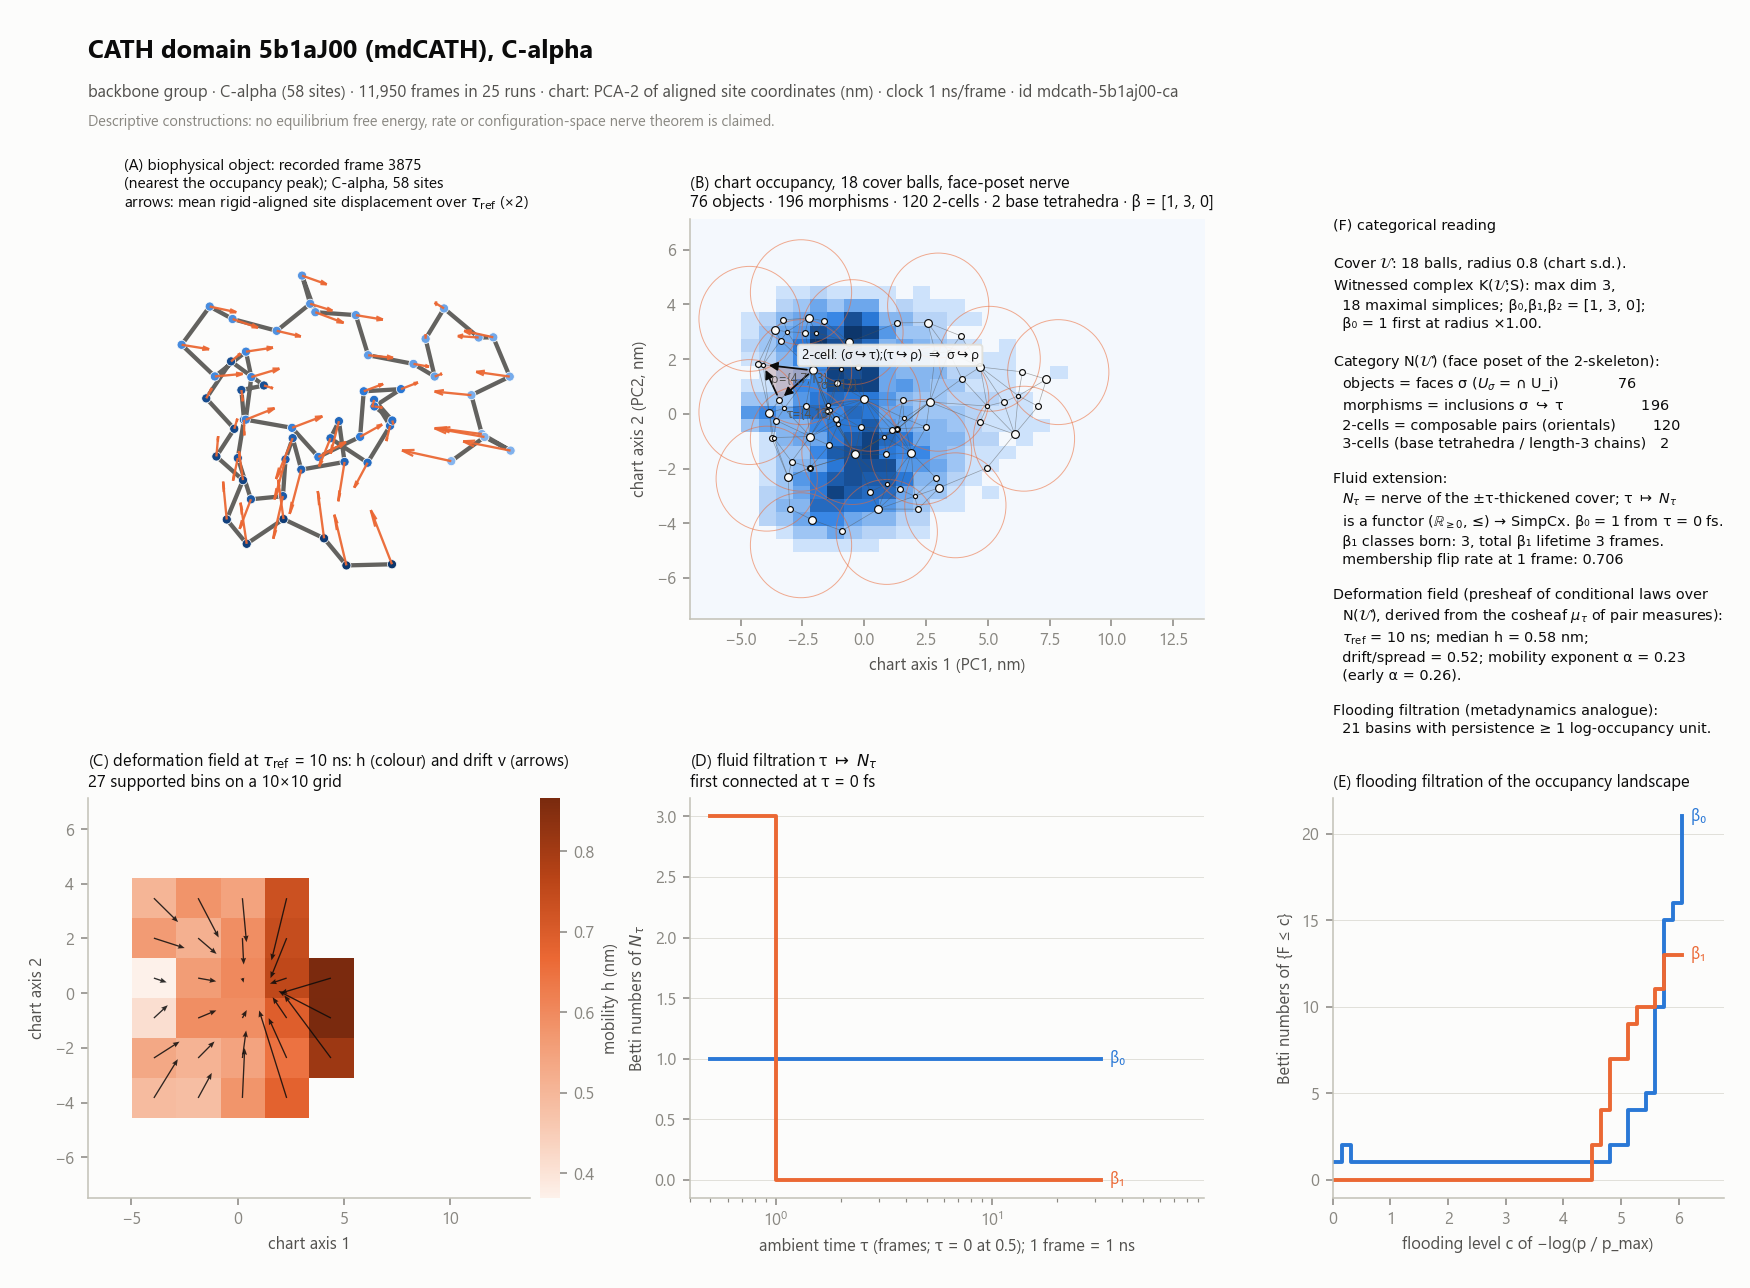
\includegraphics[width=\linewidth,height=.93\textheight,keepaspectratio]{systems/mdcath-5b1aj00-ca/plate.png}\caption{CATH domain 5b1aJ00 (mdCATH), C-alpha (\texttt{mdcath-5b1aj00-ca}). Source: https://huggingface.co/datasets/compsciencelab/mdCATH/resolve/main/data/mdcath\_dataset\_5b1aJ00.h5.}\end{figure}\clearpage
\begin{figure}[H]\centering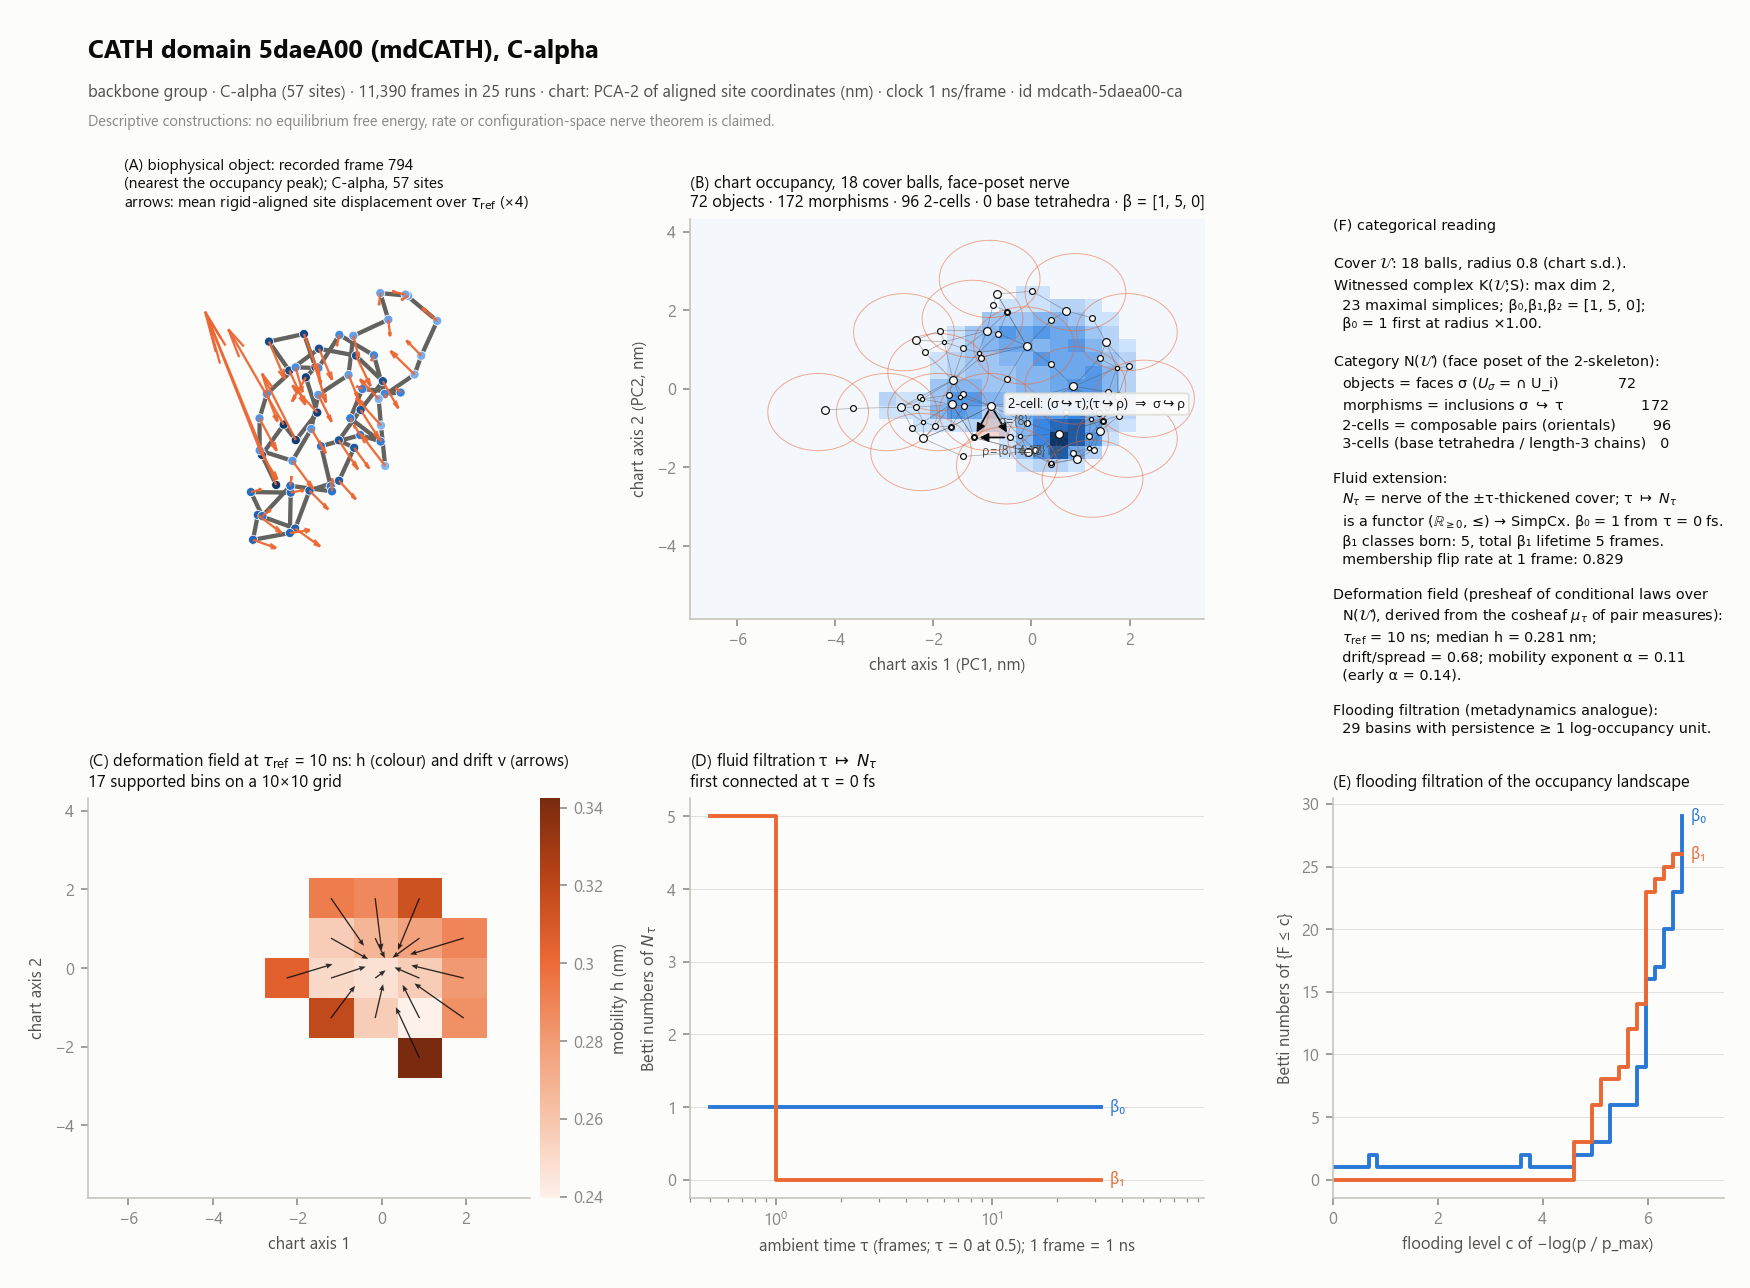
\includegraphics[width=\linewidth,height=.93\textheight,keepaspectratio]{systems/mdcath-5daea00-ca/plate.png}\caption{CATH domain 5daeA00 (mdCATH), C-alpha (\texttt{mdcath-5daea00-ca}). Source: https://huggingface.co/datasets/compsciencelab/mdCATH/resolve/main/data/mdcath\_dataset\_5daeA00.h5.}\end{figure}\clearpage
\section*{Paired heavy-atom representations of the backbone systems}
\begin{figure}[H]\centering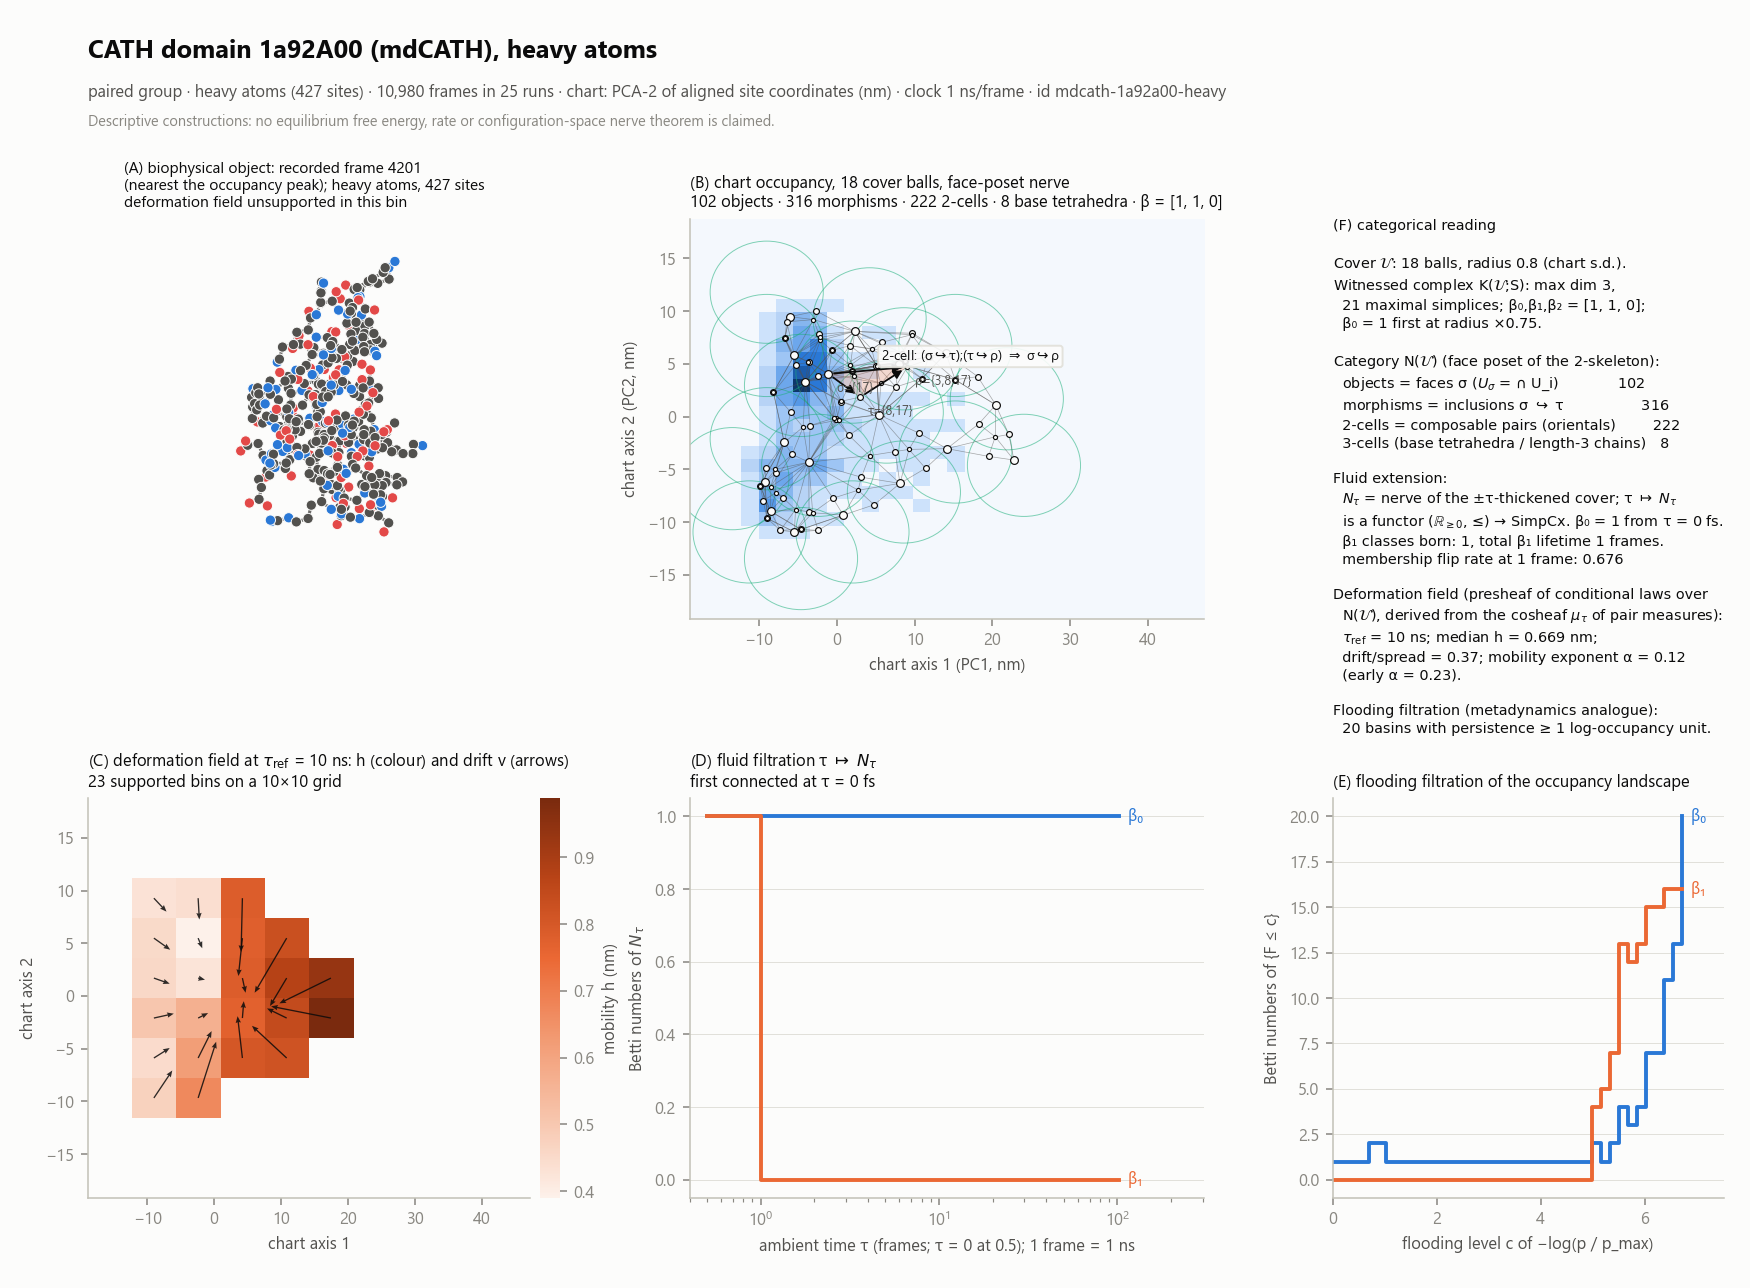
\includegraphics[width=\linewidth,height=.93\textheight,keepaspectratio]{systems/mdcath-1a92a00-heavy/plate.png}\caption{CATH domain 1a92A00 (mdCATH), heavy atoms (\texttt{mdcath-1a92a00-heavy}), paired with \texttt{mdcath-1a92a00-ca}.}\end{figure}\clearpage
\begin{figure}[H]\centering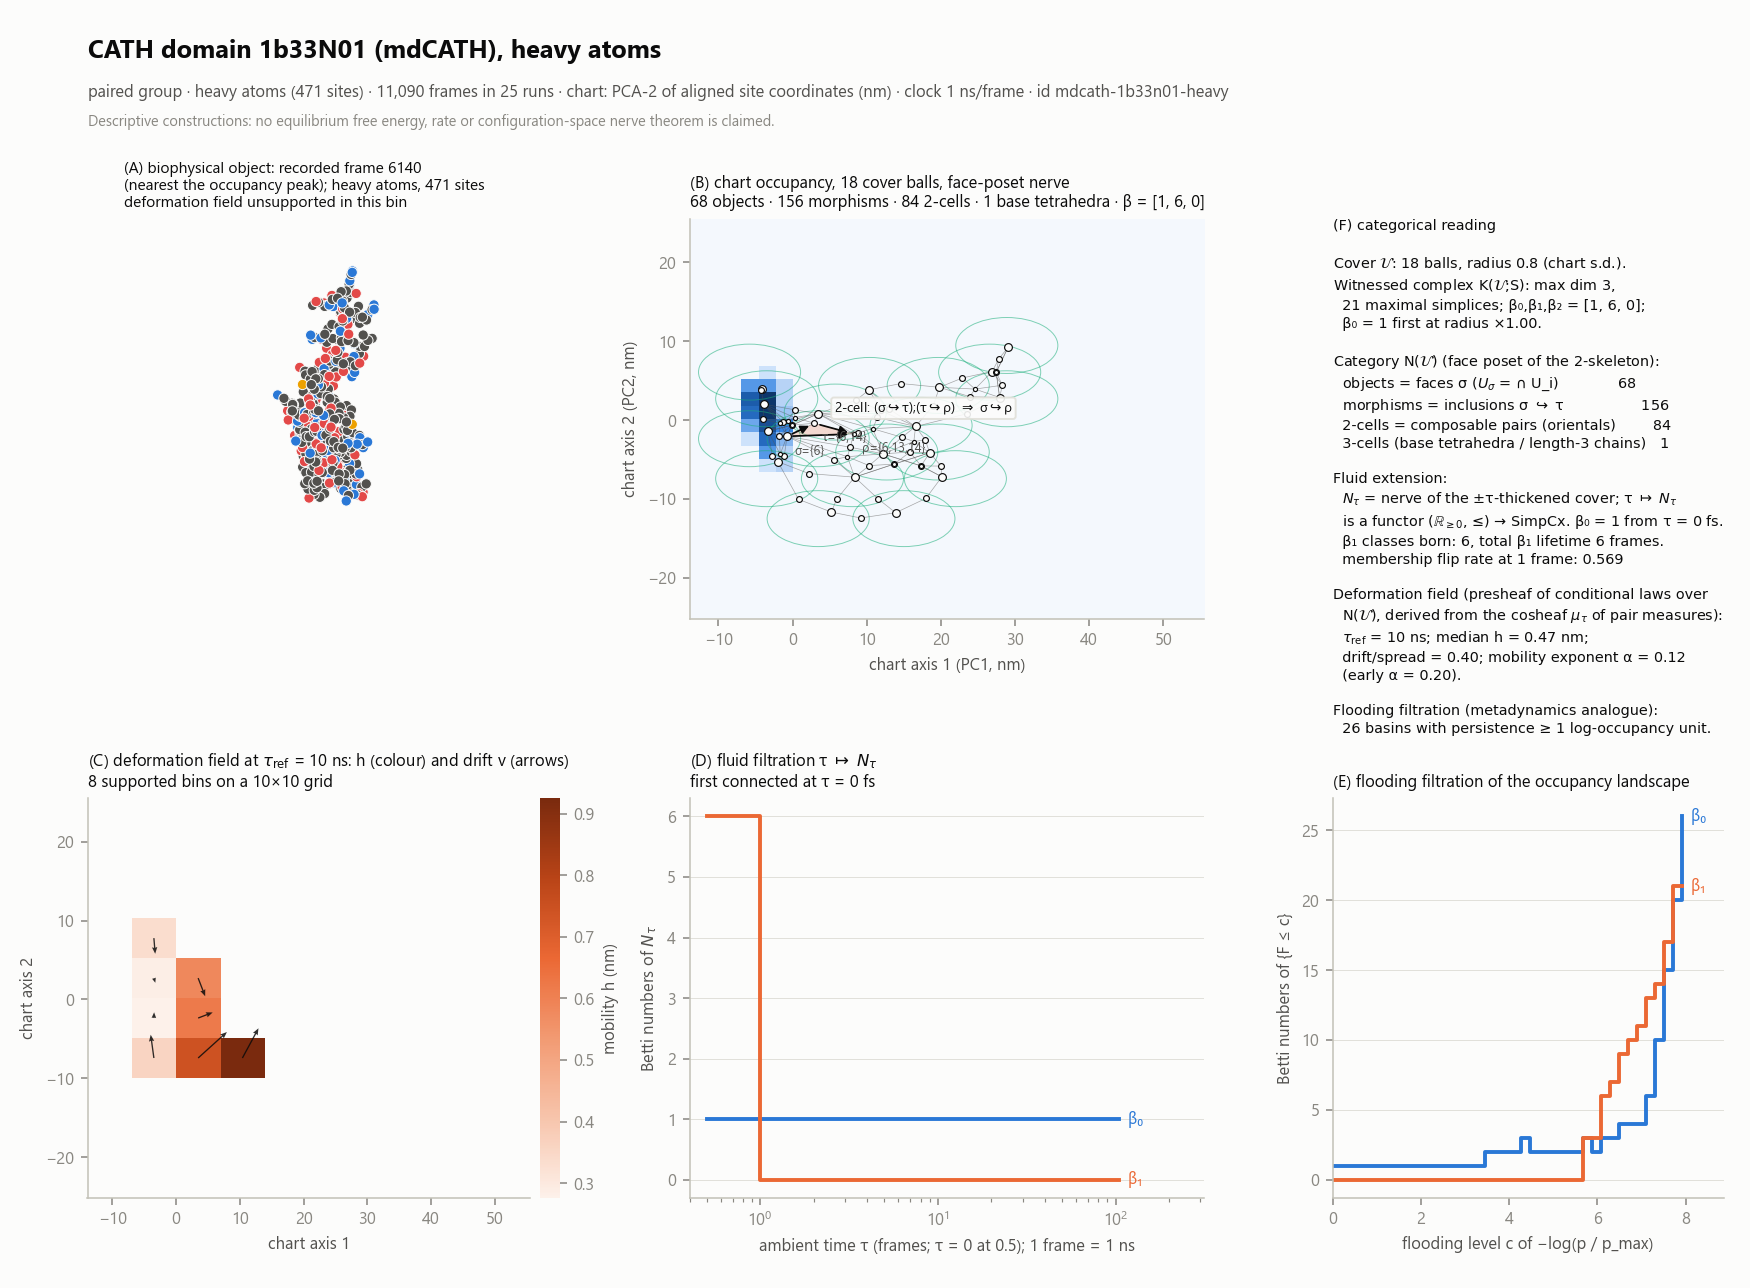
\includegraphics[width=\linewidth,height=.93\textheight,keepaspectratio]{systems/mdcath-1b33n01-heavy/plate.png}\caption{CATH domain 1b33N01 (mdCATH), heavy atoms (\texttt{mdcath-1b33n01-heavy}), paired with \texttt{mdcath-1b33n01-ca}.}\end{figure}\clearpage
\begin{figure}[H]\centering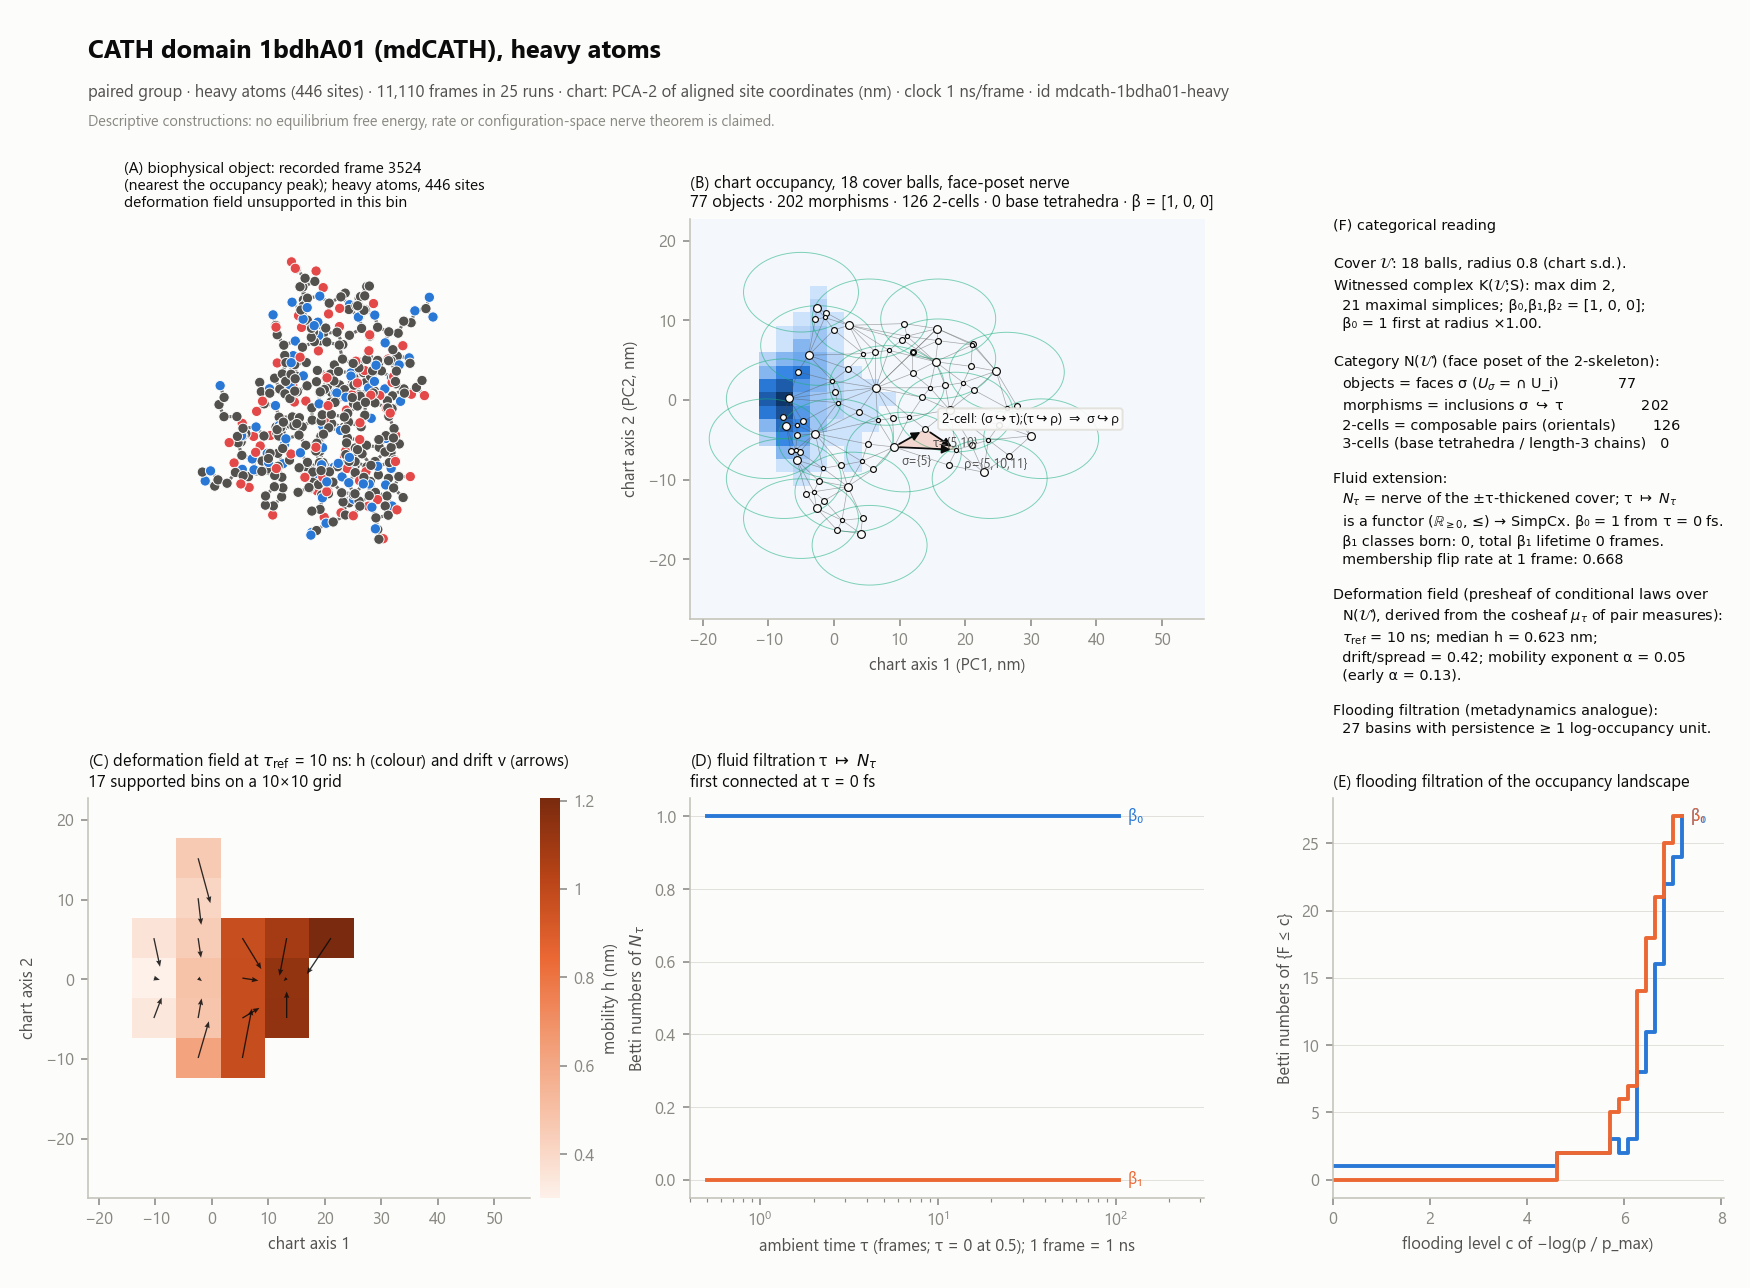
\includegraphics[width=\linewidth,height=.93\textheight,keepaspectratio]{systems/mdcath-1bdha01-heavy/plate.png}\caption{CATH domain 1bdhA01 (mdCATH), heavy atoms (\texttt{mdcath-1bdha01-heavy}), paired with \texttt{mdcath-1bdha01-ca}.}\end{figure}\clearpage
\begin{figure}[H]\centering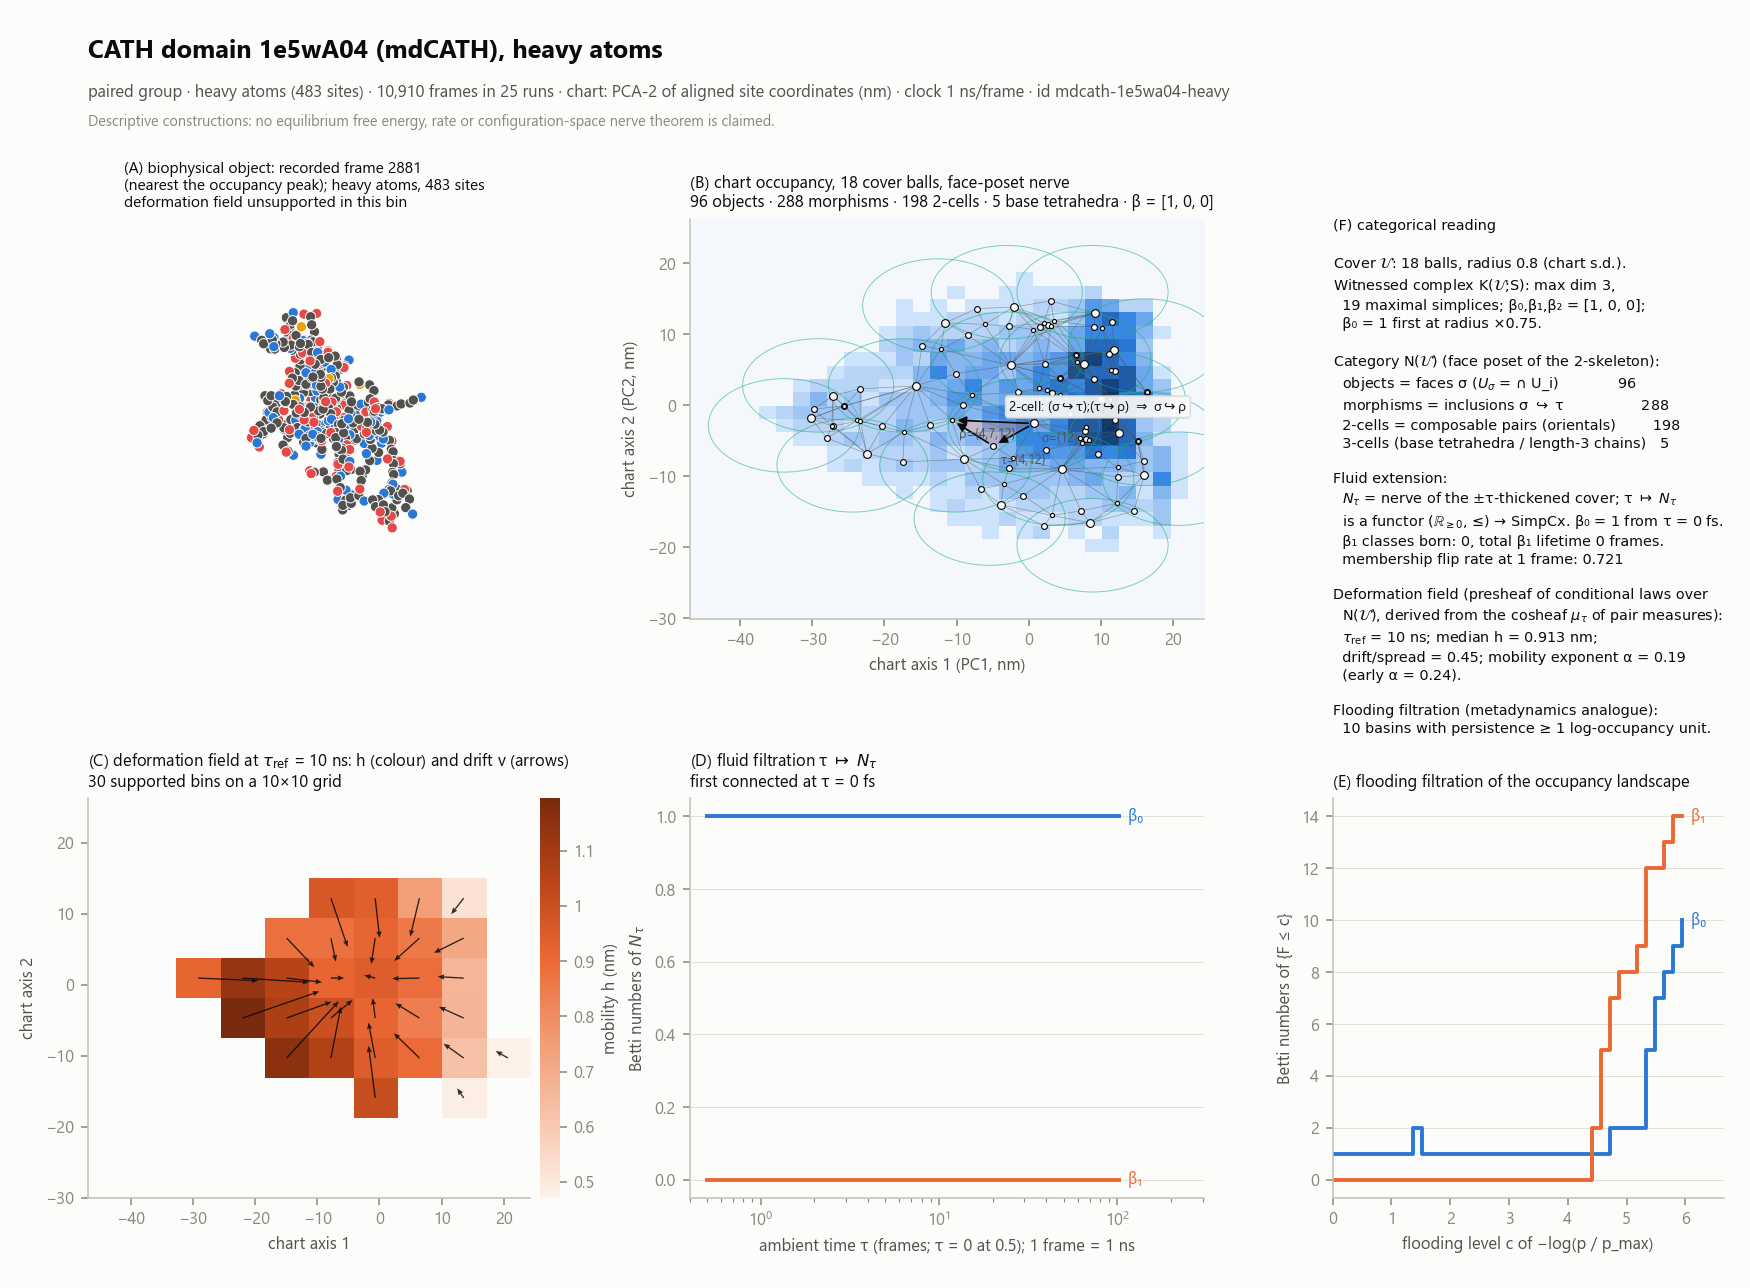
\includegraphics[width=\linewidth,height=.93\textheight,keepaspectratio]{systems/mdcath-1e5wa04-heavy/plate.png}\caption{CATH domain 1e5wA04 (mdCATH), heavy atoms (\texttt{mdcath-1e5wa04-heavy}), paired with \texttt{mdcath-1e5wa04-ca}.}\end{figure}\clearpage
\begin{figure}[H]\centering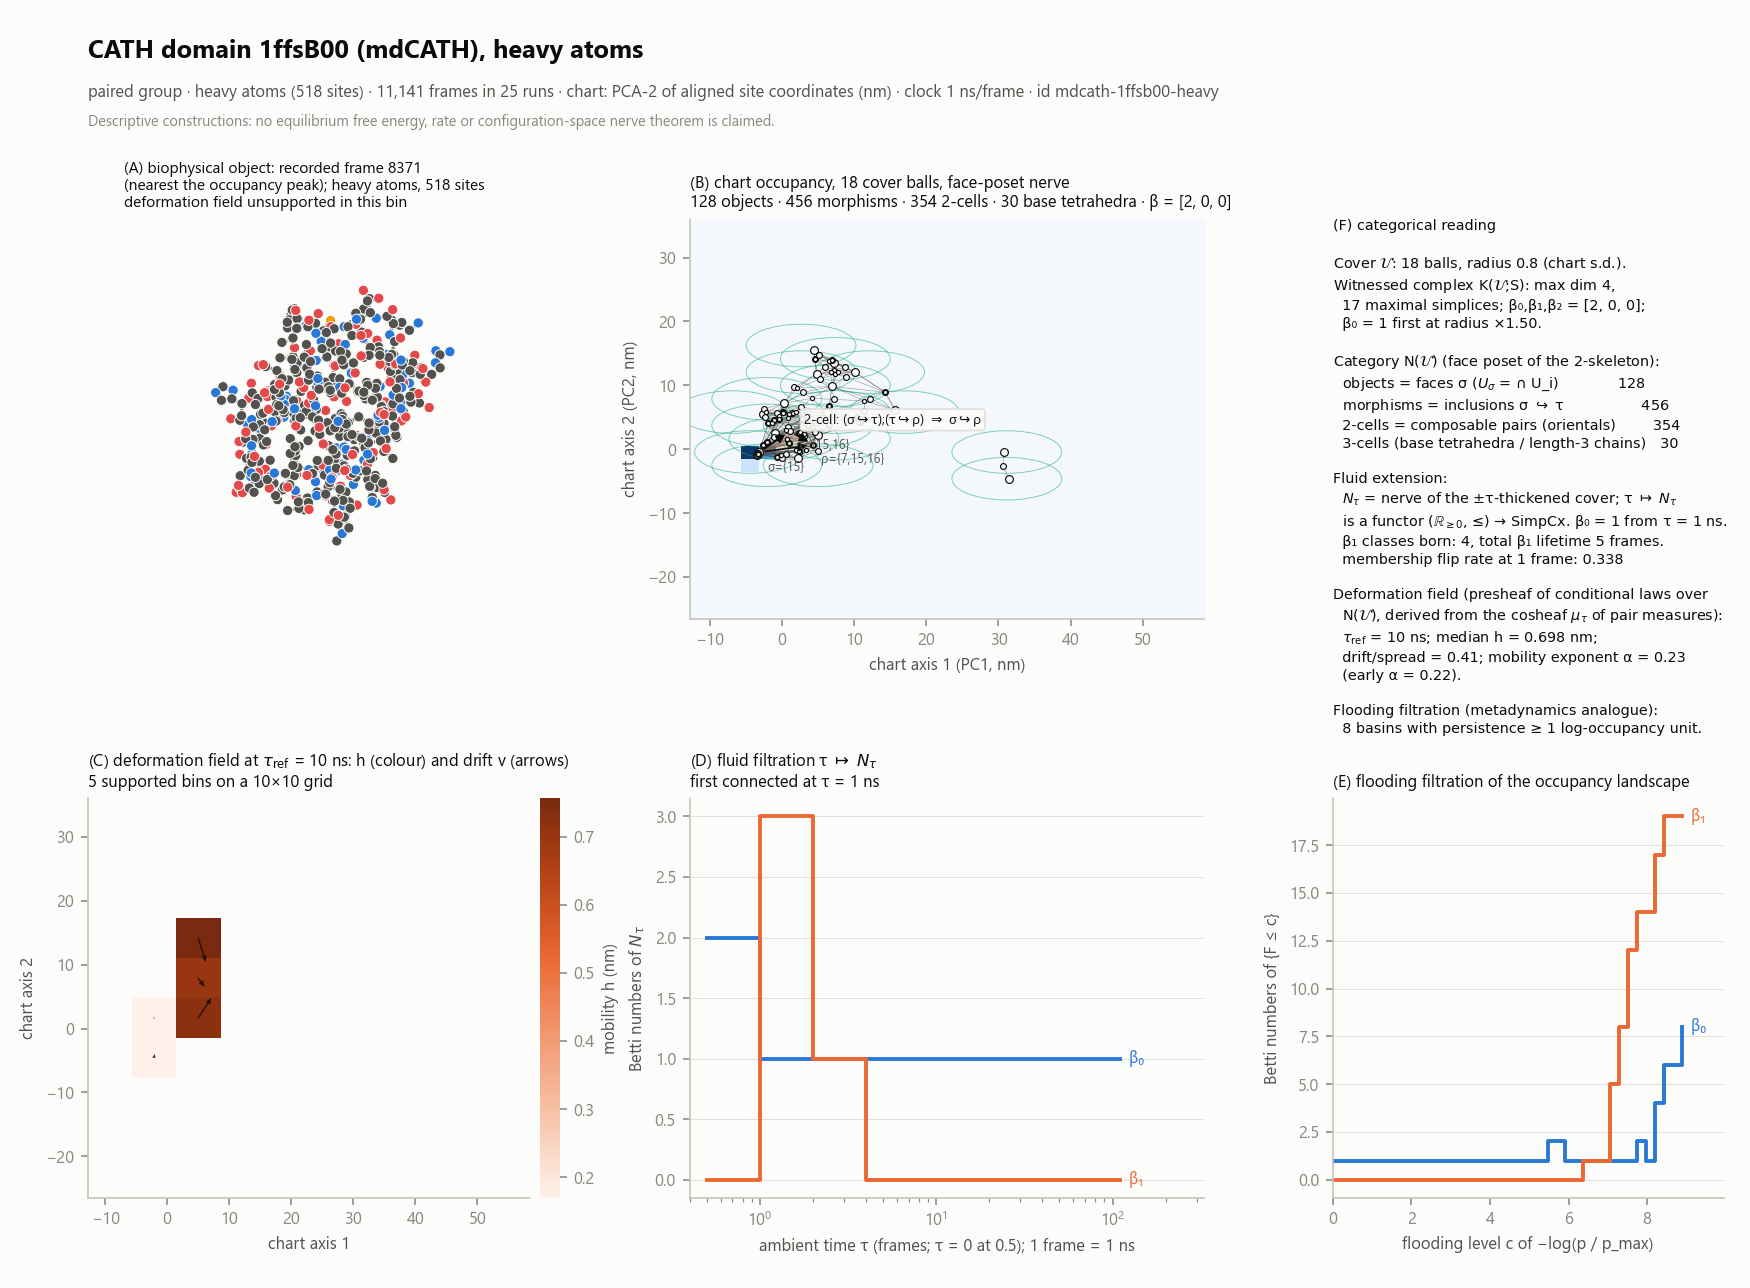
\includegraphics[width=\linewidth,height=.93\textheight,keepaspectratio]{systems/mdcath-1ffsb00-heavy/plate.png}\caption{CATH domain 1ffsB00 (mdCATH), heavy atoms (\texttt{mdcath-1ffsb00-heavy}), paired with \texttt{mdcath-1ffsb00-ca}.}\end{figure}\clearpage
\begin{figure}[H]\centering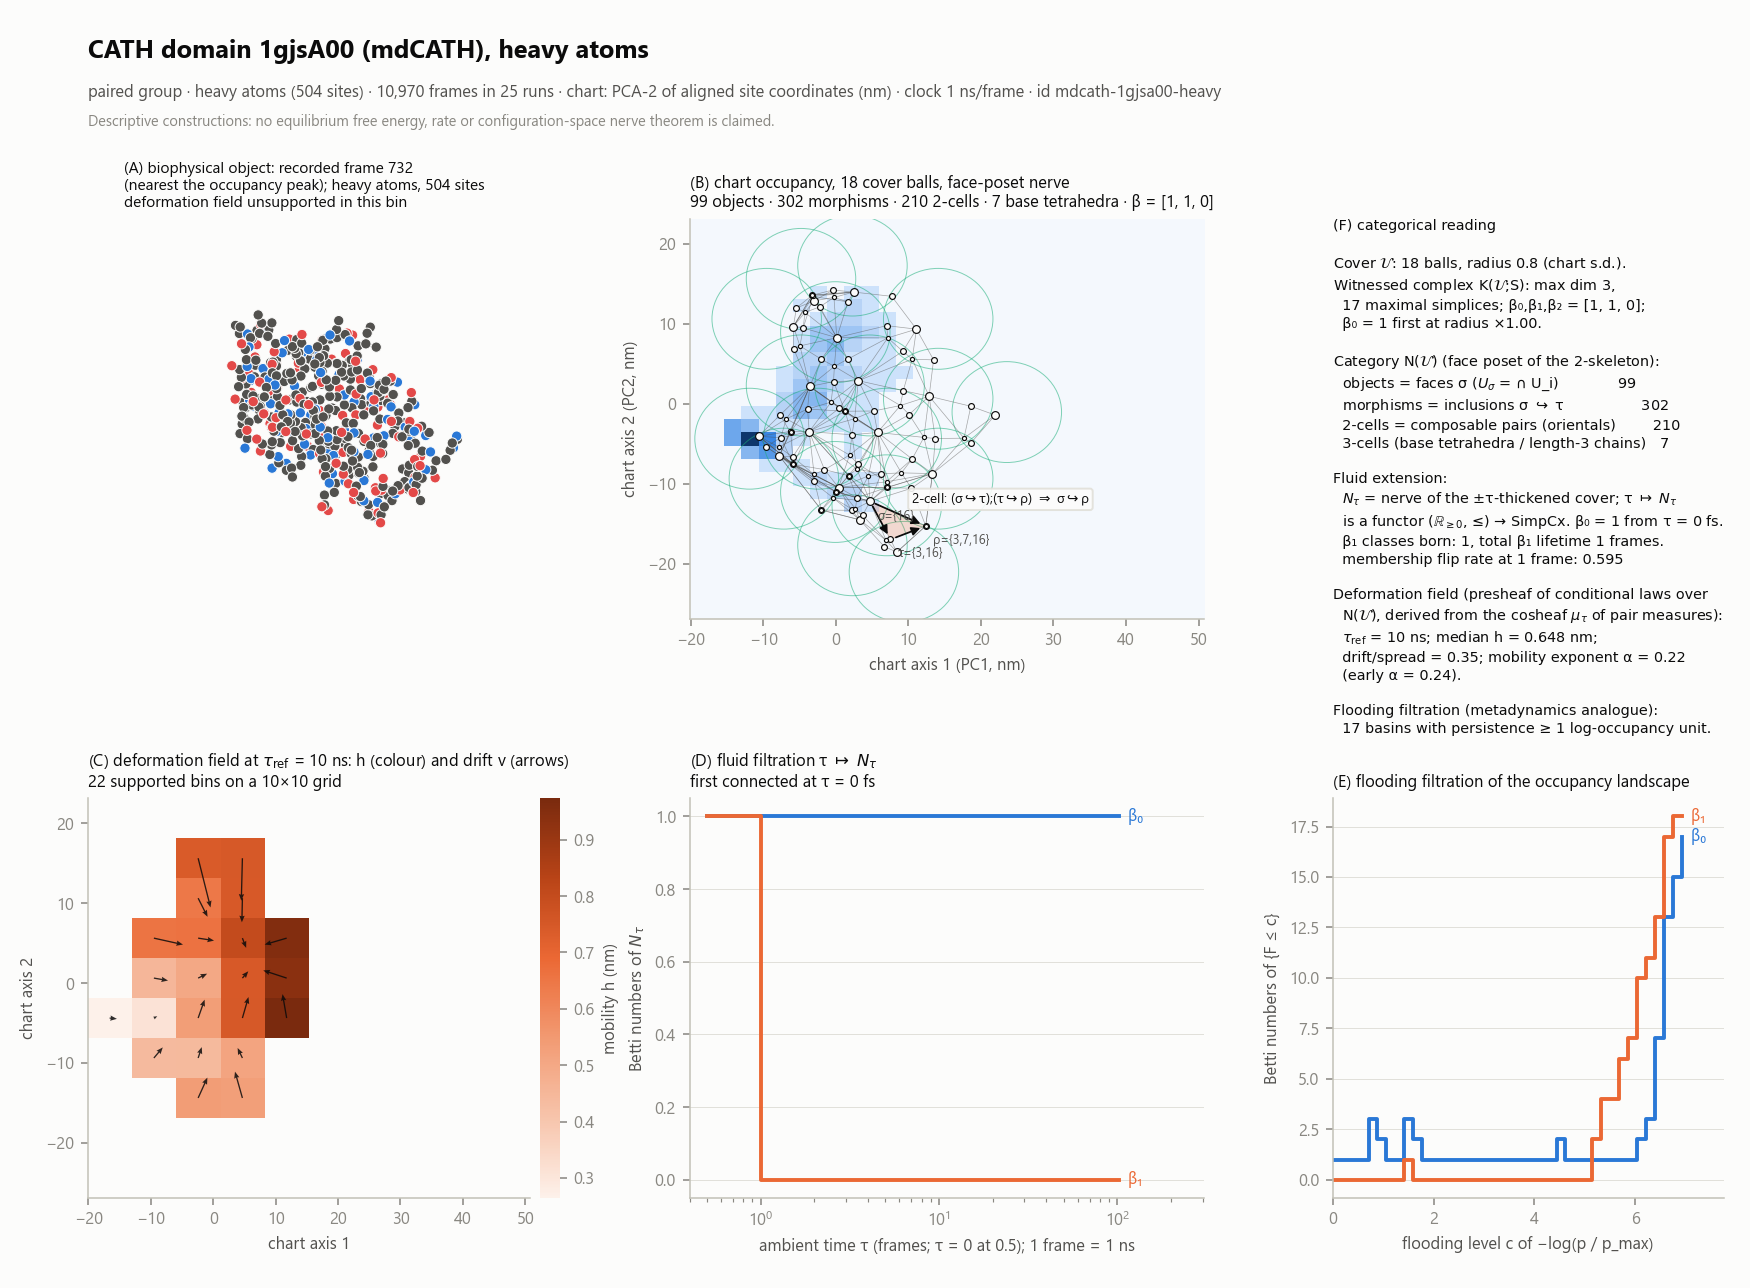
\includegraphics[width=\linewidth,height=.93\textheight,keepaspectratio]{systems/mdcath-1gjsa00-heavy/plate.png}\caption{CATH domain 1gjsA00 (mdCATH), heavy atoms (\texttt{mdcath-1gjsa00-heavy}), paired with \texttt{mdcath-1gjsa00-ca}.}\end{figure}\clearpage
\begin{figure}[H]\centering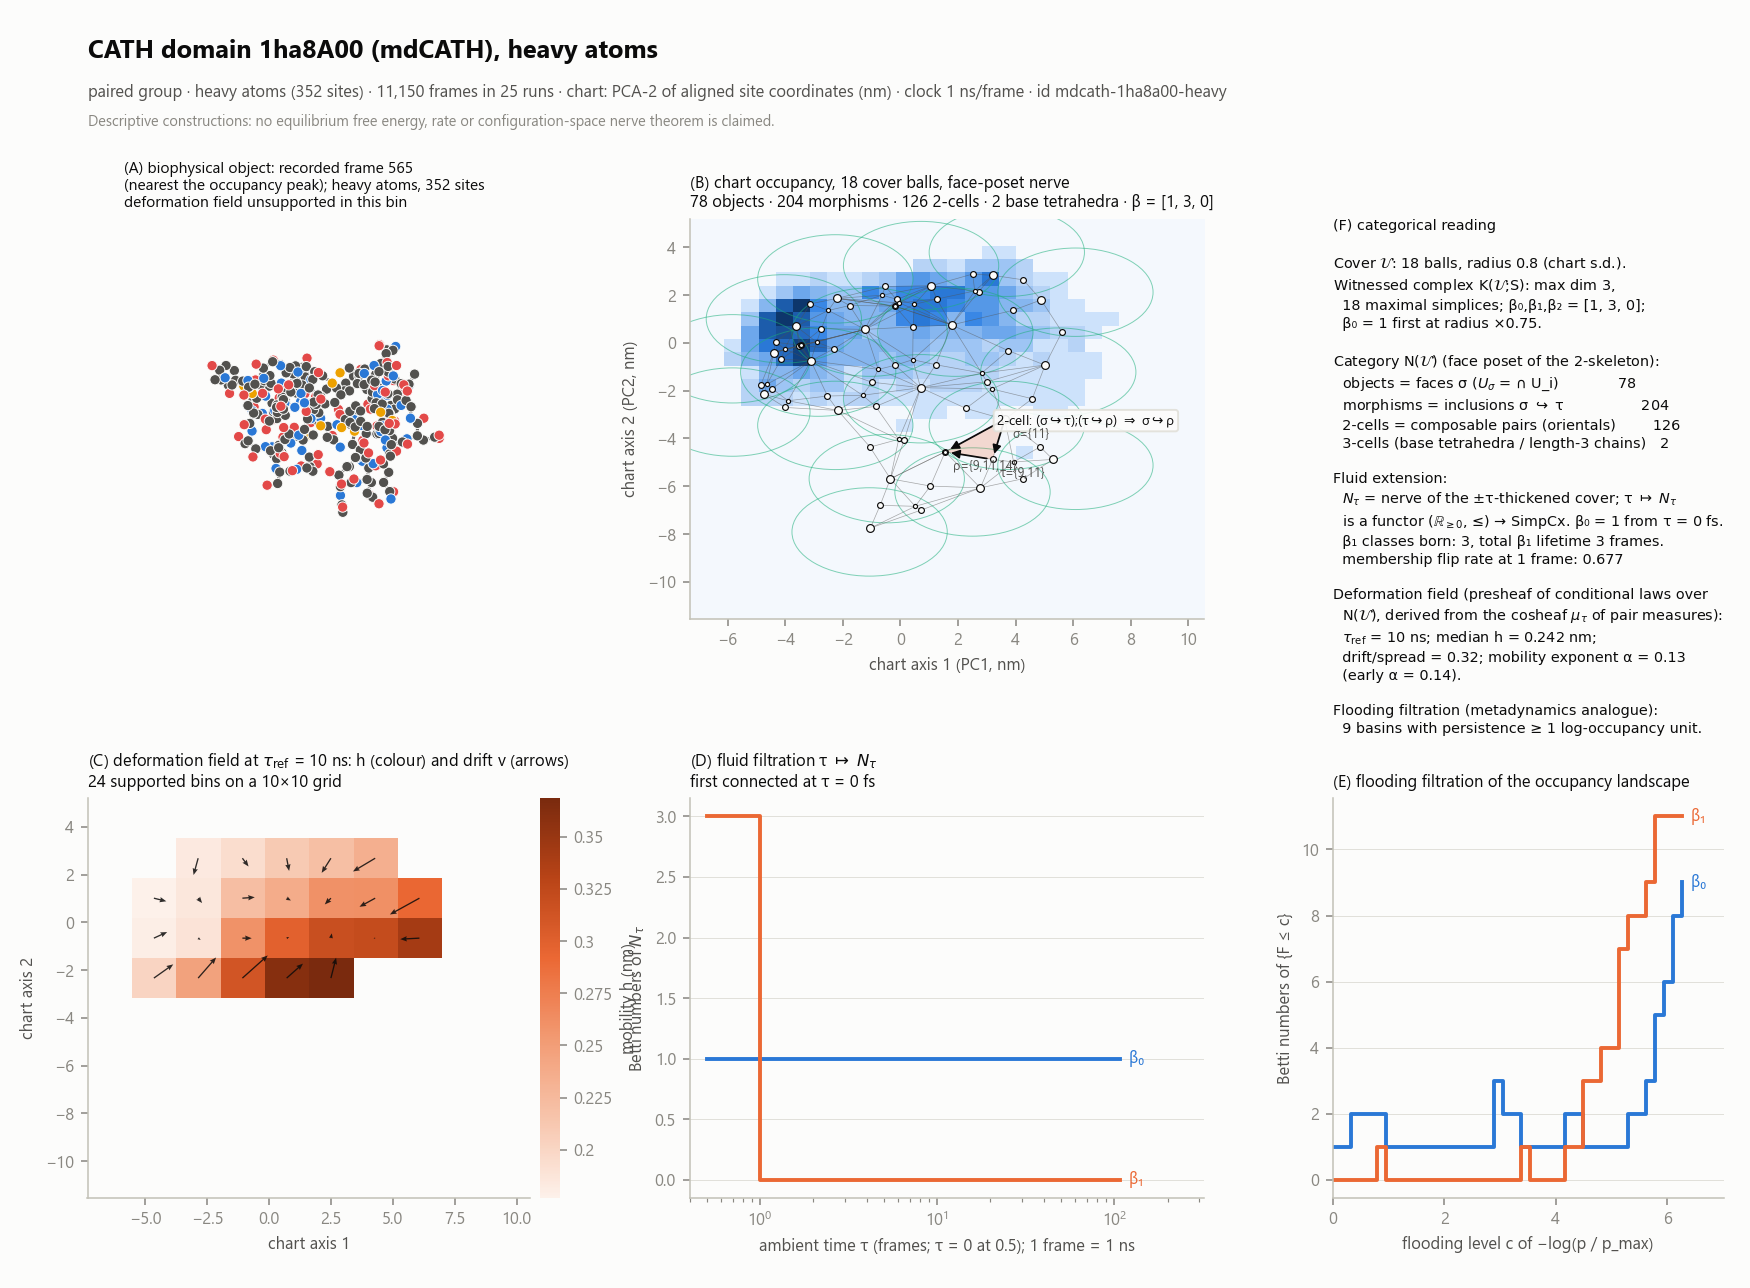
\includegraphics[width=\linewidth,height=.93\textheight,keepaspectratio]{systems/mdcath-1ha8a00-heavy/plate.png}\caption{CATH domain 1ha8A00 (mdCATH), heavy atoms (\texttt{mdcath-1ha8a00-heavy}), paired with \texttt{mdcath-1ha8a00-ca}.}\end{figure}\clearpage
\begin{figure}[H]\centering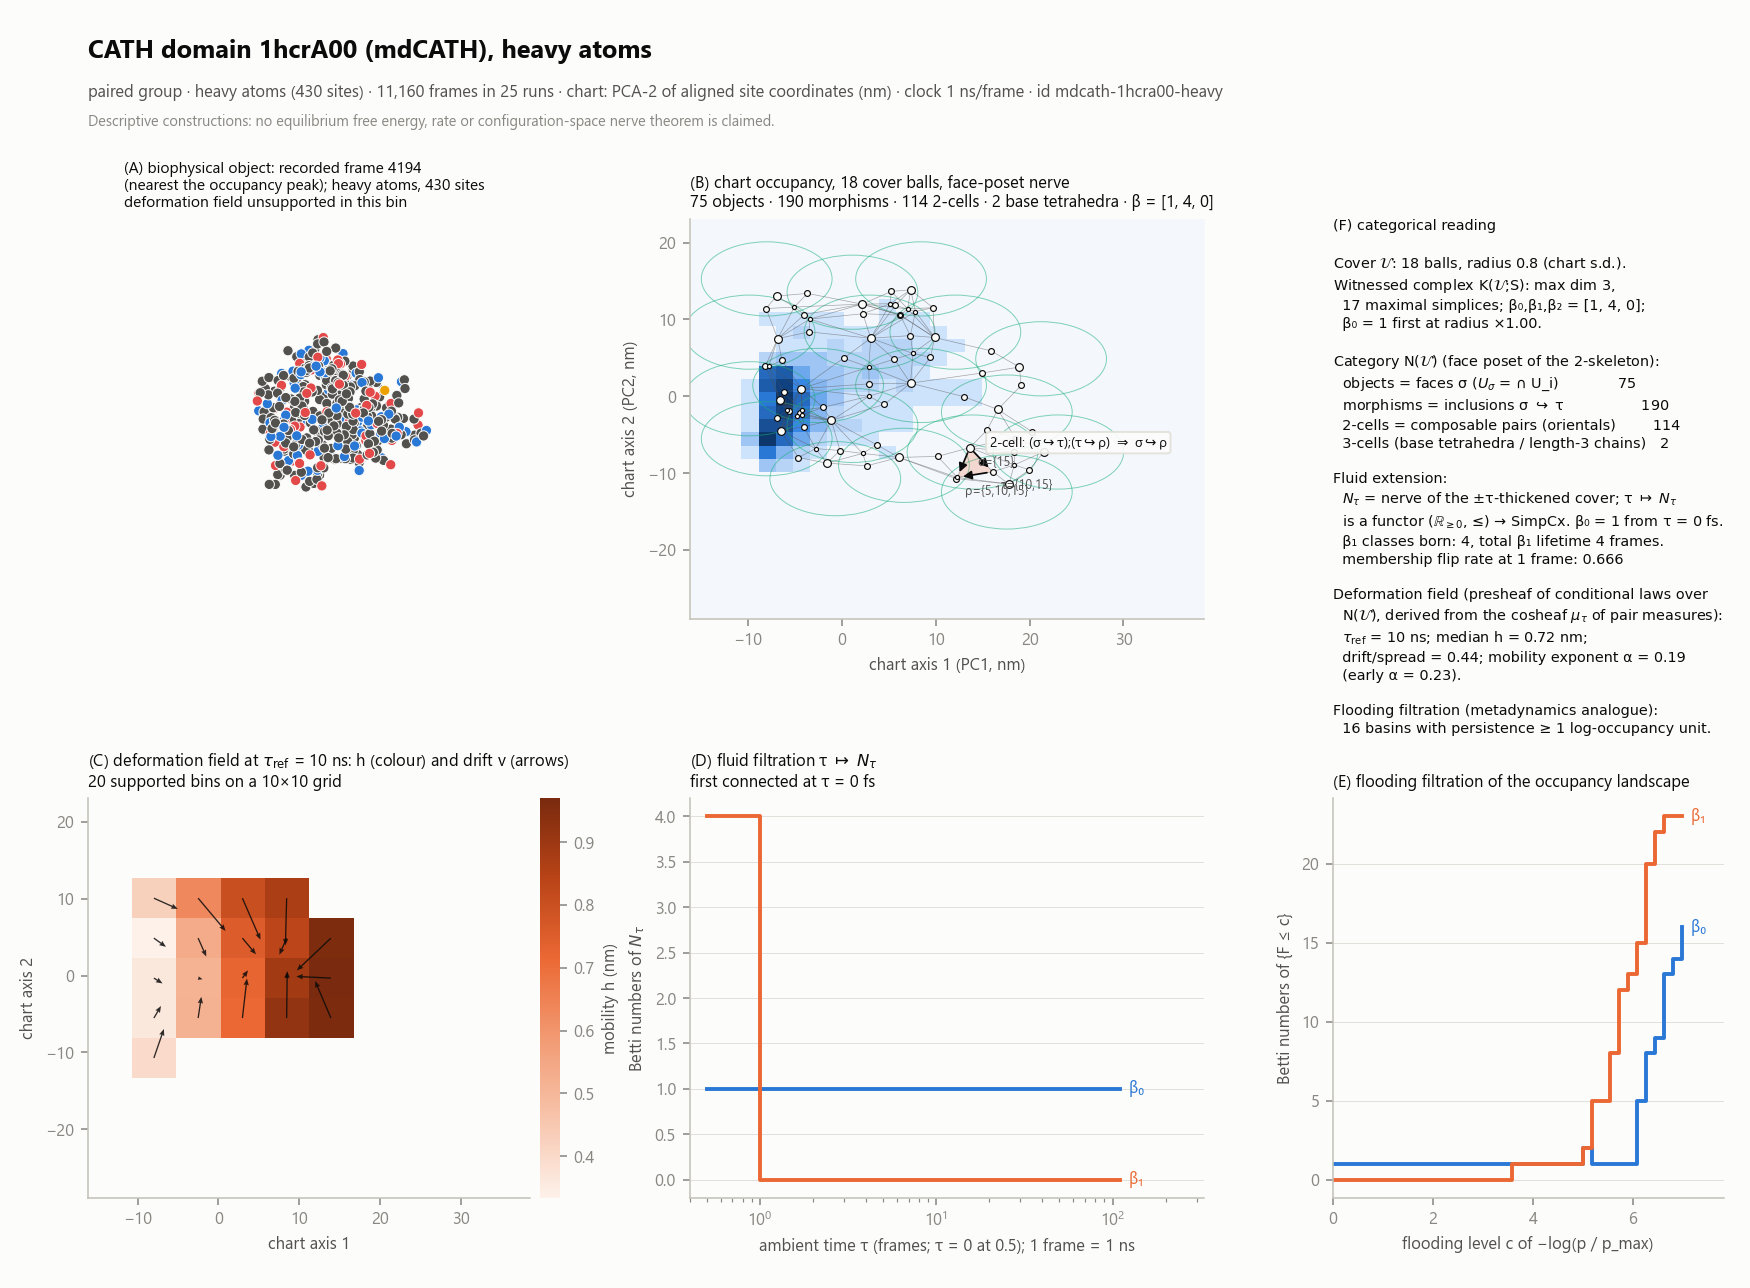
\includegraphics[width=\linewidth,height=.93\textheight,keepaspectratio]{systems/mdcath-1hcra00-heavy/plate.png}\caption{CATH domain 1hcrA00 (mdCATH), heavy atoms (\texttt{mdcath-1hcra00-heavy}), paired with \texttt{mdcath-1hcra00-ca}.}\end{figure}\clearpage
\begin{figure}[H]\centering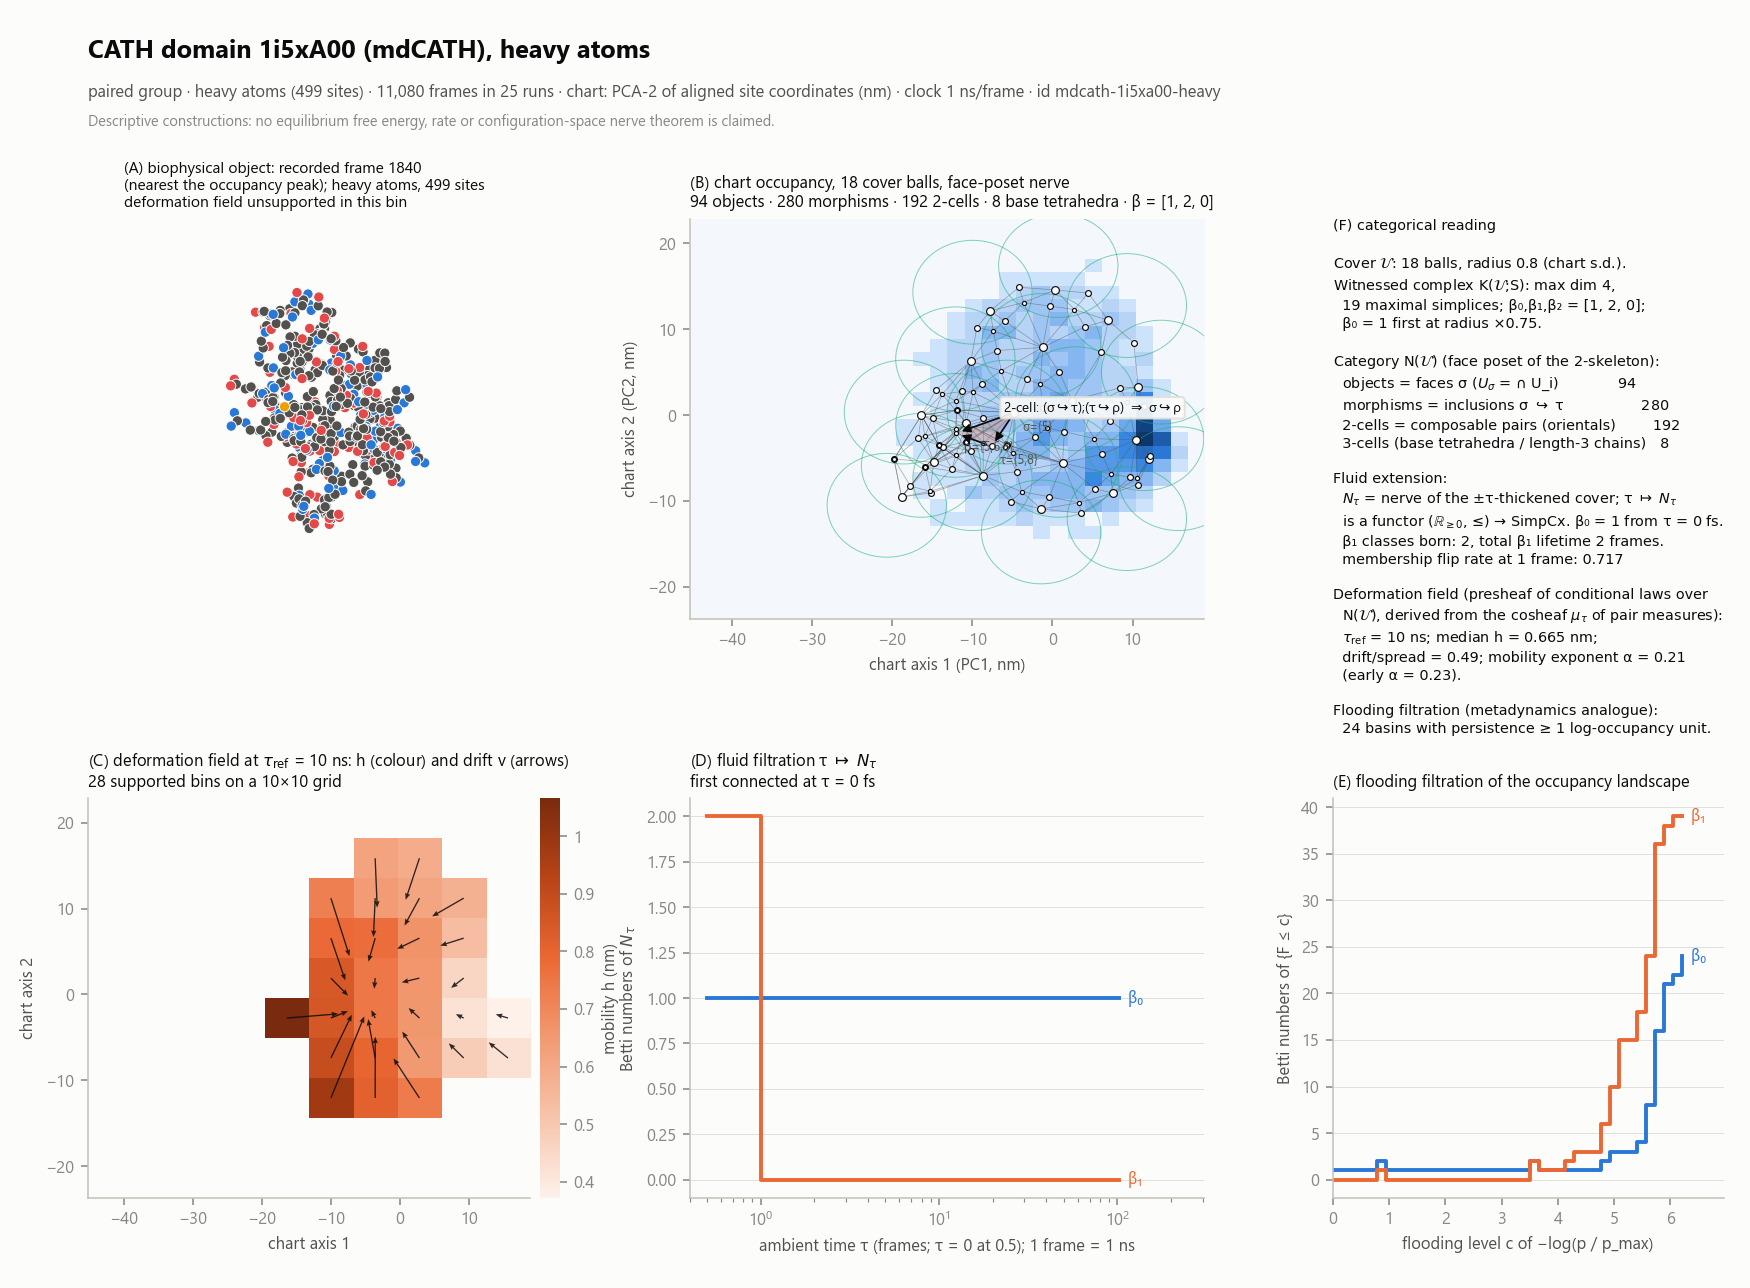
\includegraphics[width=\linewidth,height=.93\textheight,keepaspectratio]{systems/mdcath-1i5xa00-heavy/plate.png}\caption{CATH domain 1i5xA00 (mdCATH), heavy atoms (\texttt{mdcath-1i5xa00-heavy}), paired with \texttt{mdcath-1i5xa00-ca}.}\end{figure}\clearpage
\begin{figure}[H]\centering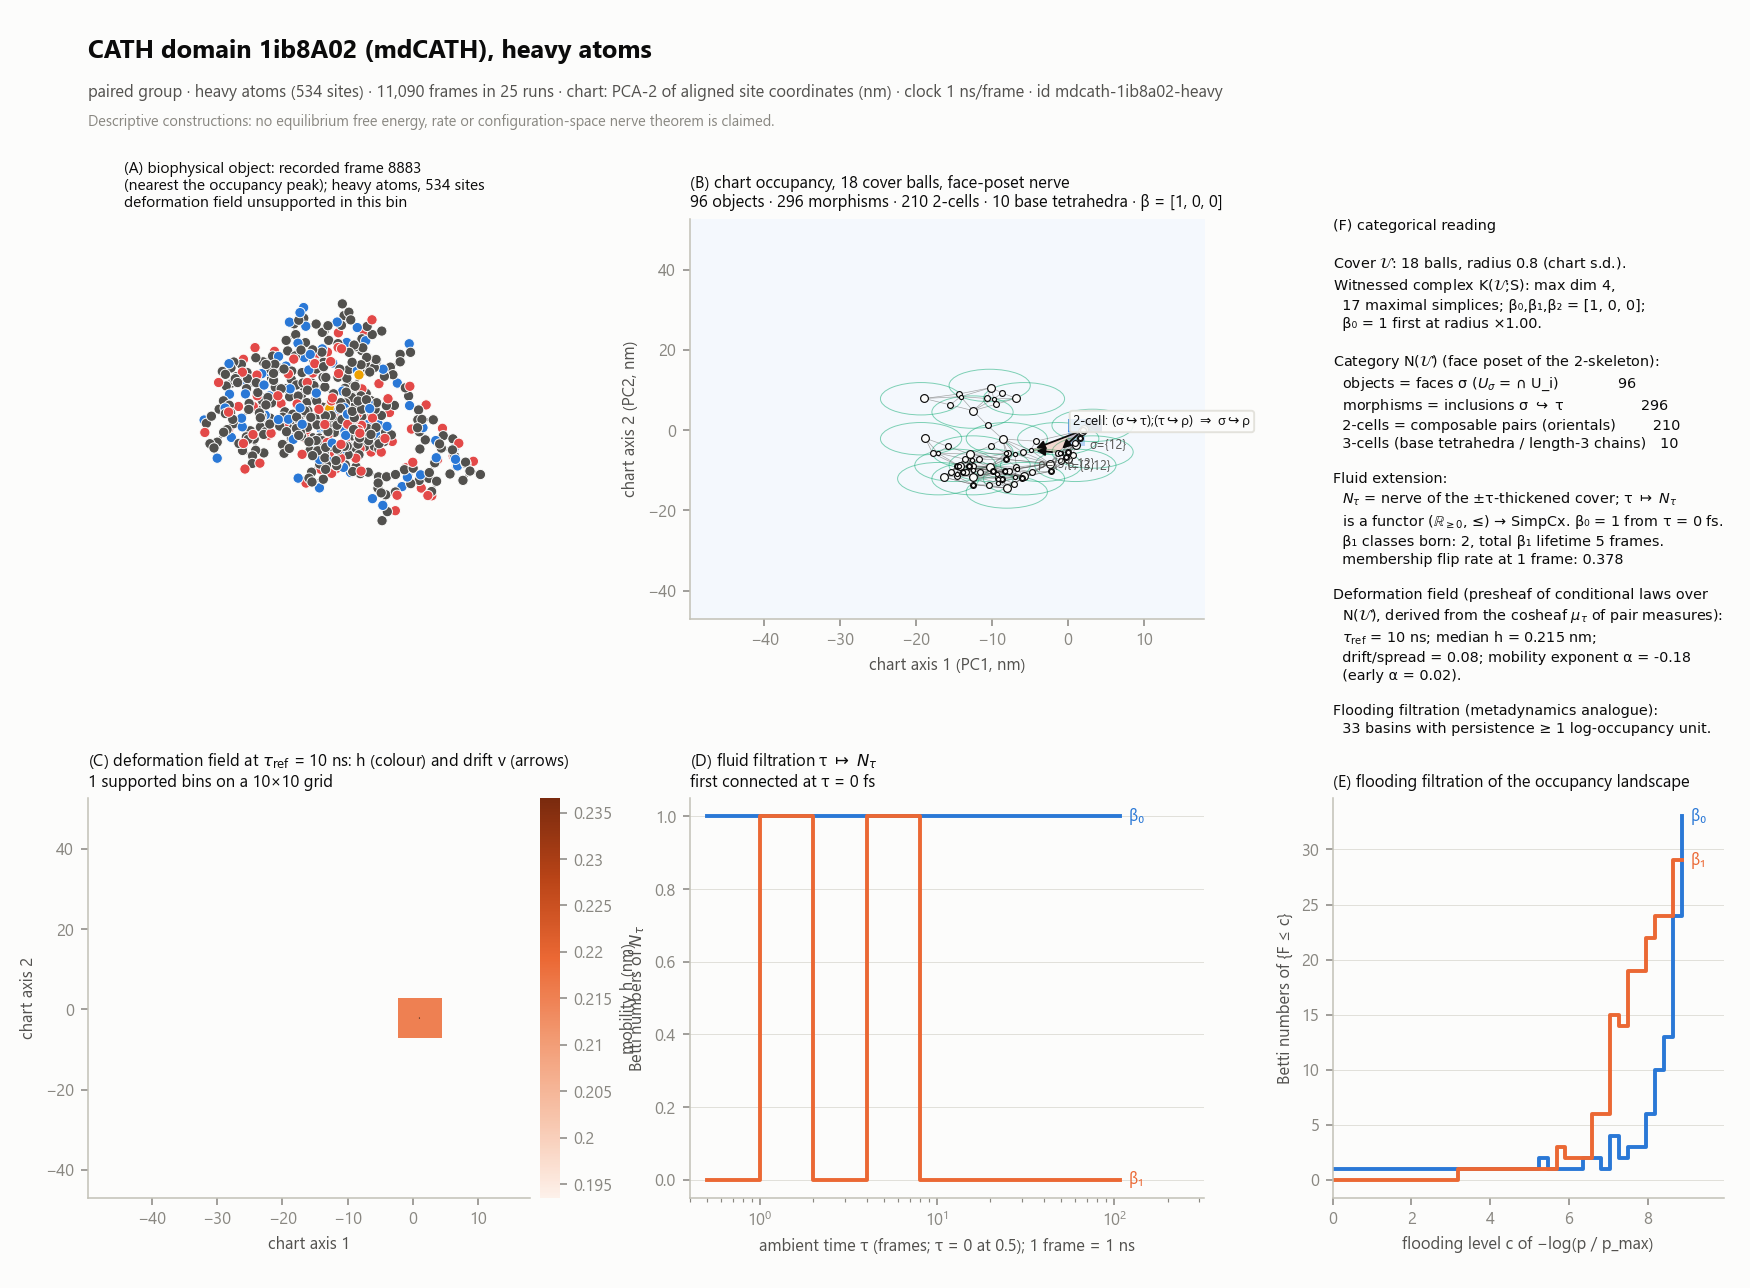
\includegraphics[width=\linewidth,height=.93\textheight,keepaspectratio]{systems/mdcath-1ib8a02-heavy/plate.png}\caption{CATH domain 1ib8A02 (mdCATH), heavy atoms (\texttt{mdcath-1ib8a02-heavy}), paired with \texttt{mdcath-1ib8a02-ca}.}\end{figure}\clearpage
\begin{figure}[H]\centering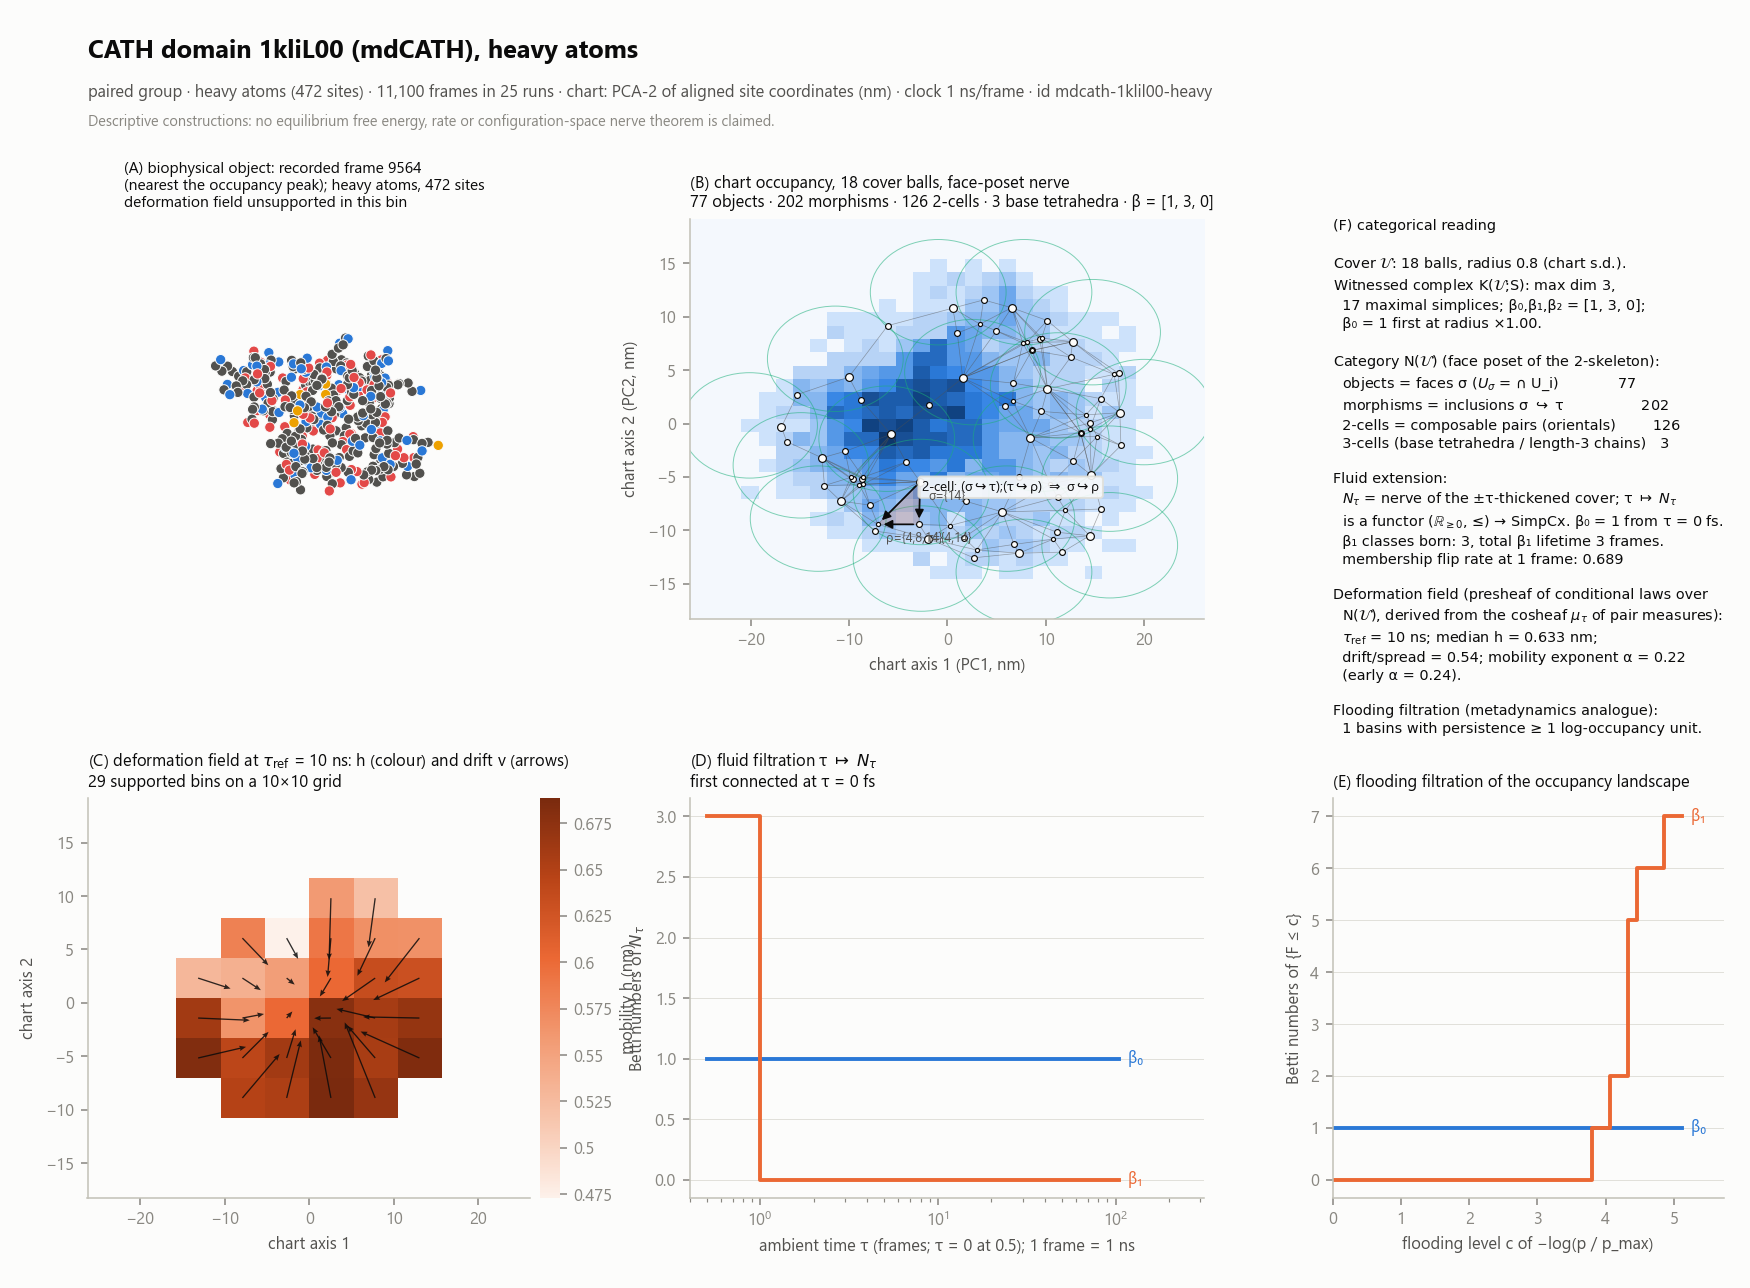
\includegraphics[width=\linewidth,height=.93\textheight,keepaspectratio]{systems/mdcath-1klil00-heavy/plate.png}\caption{CATH domain 1kliL00 (mdCATH), heavy atoms (\texttt{mdcath-1klil00-heavy}), paired with \texttt{mdcath-1klil00-ca}.}\end{figure}\clearpage
\begin{figure}[H]\centering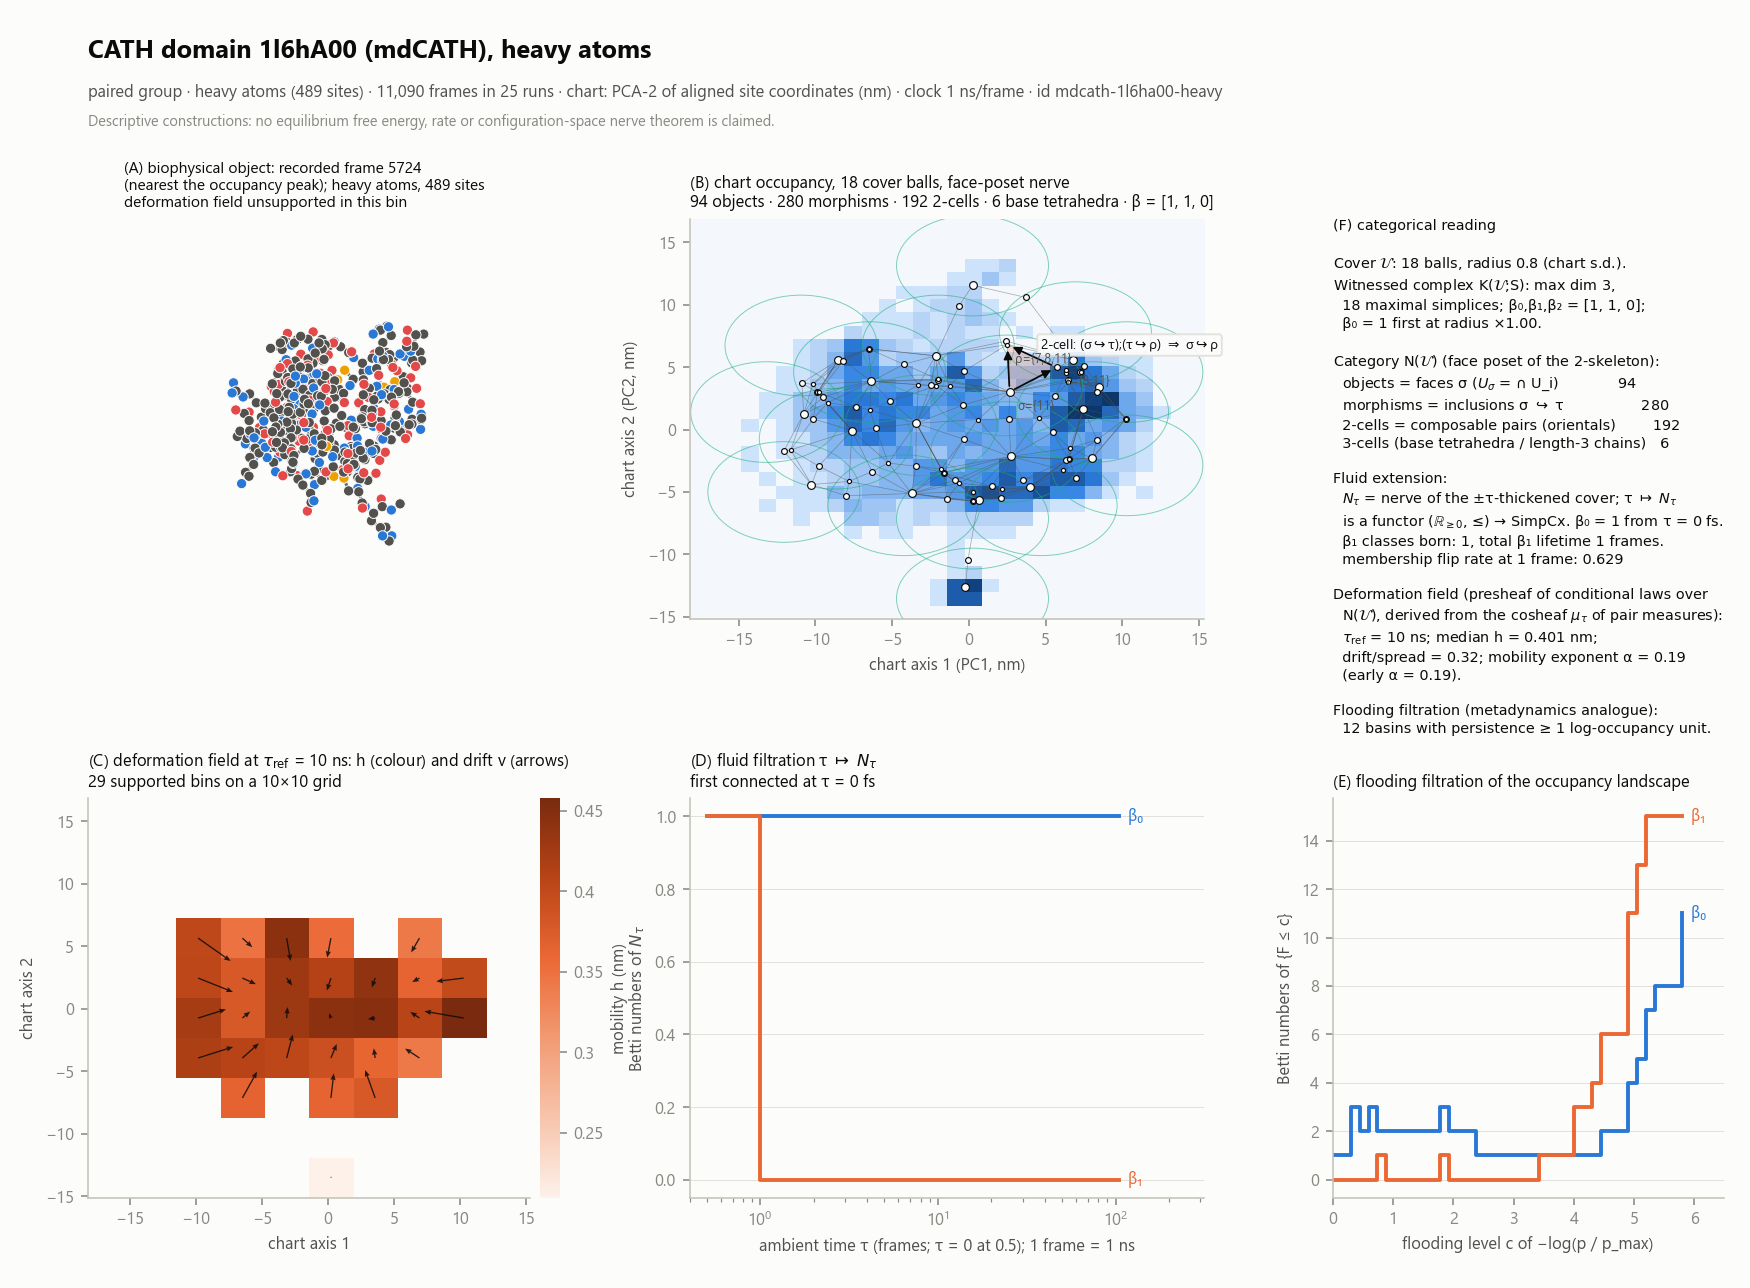
\includegraphics[width=\linewidth,height=.93\textheight,keepaspectratio]{systems/mdcath-1l6ha00-heavy/plate.png}\caption{CATH domain 1l6hA00 (mdCATH), heavy atoms (\texttt{mdcath-1l6ha00-heavy}), paired with \texttt{mdcath-1l6ha00-ca}.}\end{figure}\clearpage
\begin{figure}[H]\centering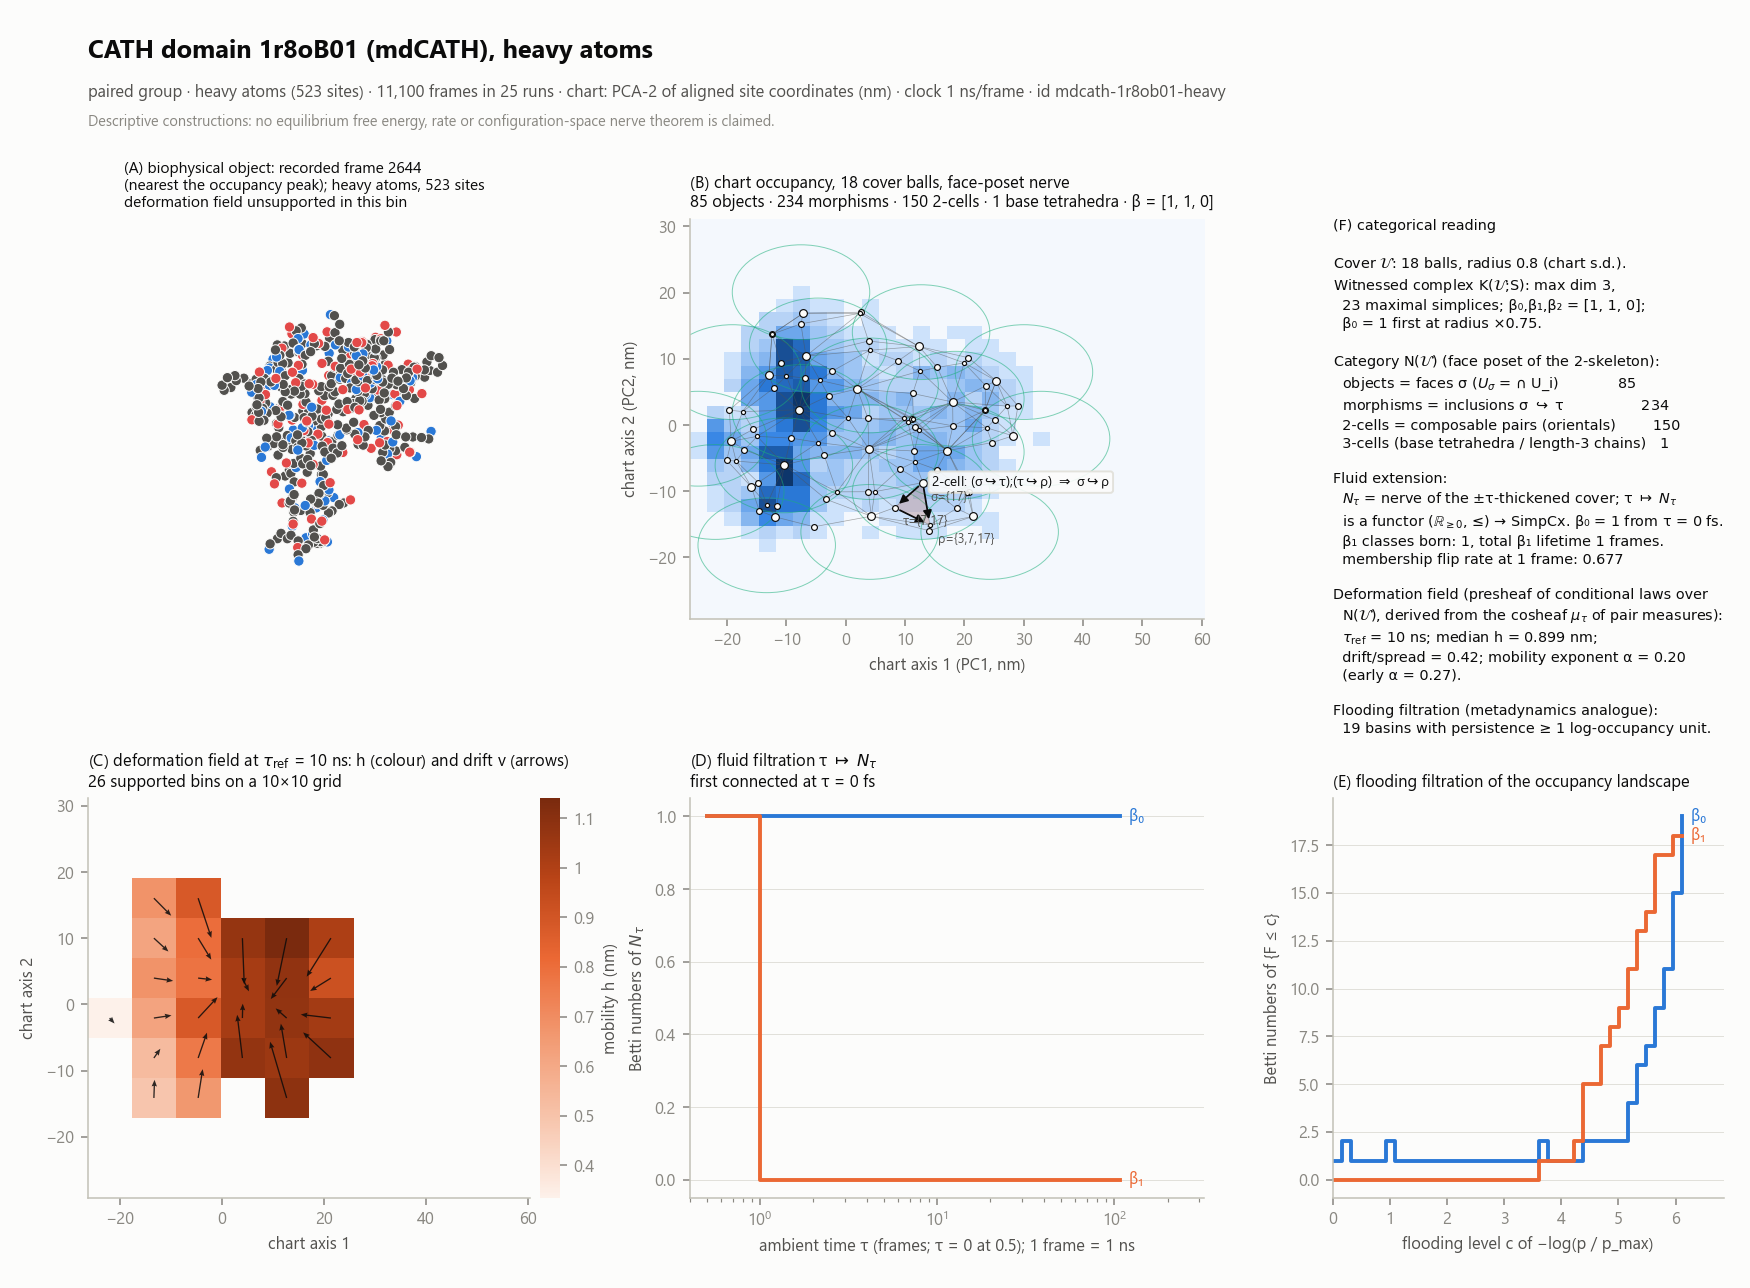
\includegraphics[width=\linewidth,height=.93\textheight,keepaspectratio]{systems/mdcath-1r8ob01-heavy/plate.png}\caption{CATH domain 1r8oB01 (mdCATH), heavy atoms (\texttt{mdcath-1r8ob01-heavy}), paired with \texttt{mdcath-1r8ob01-ca}.}\end{figure}\clearpage
\begin{figure}[H]\centering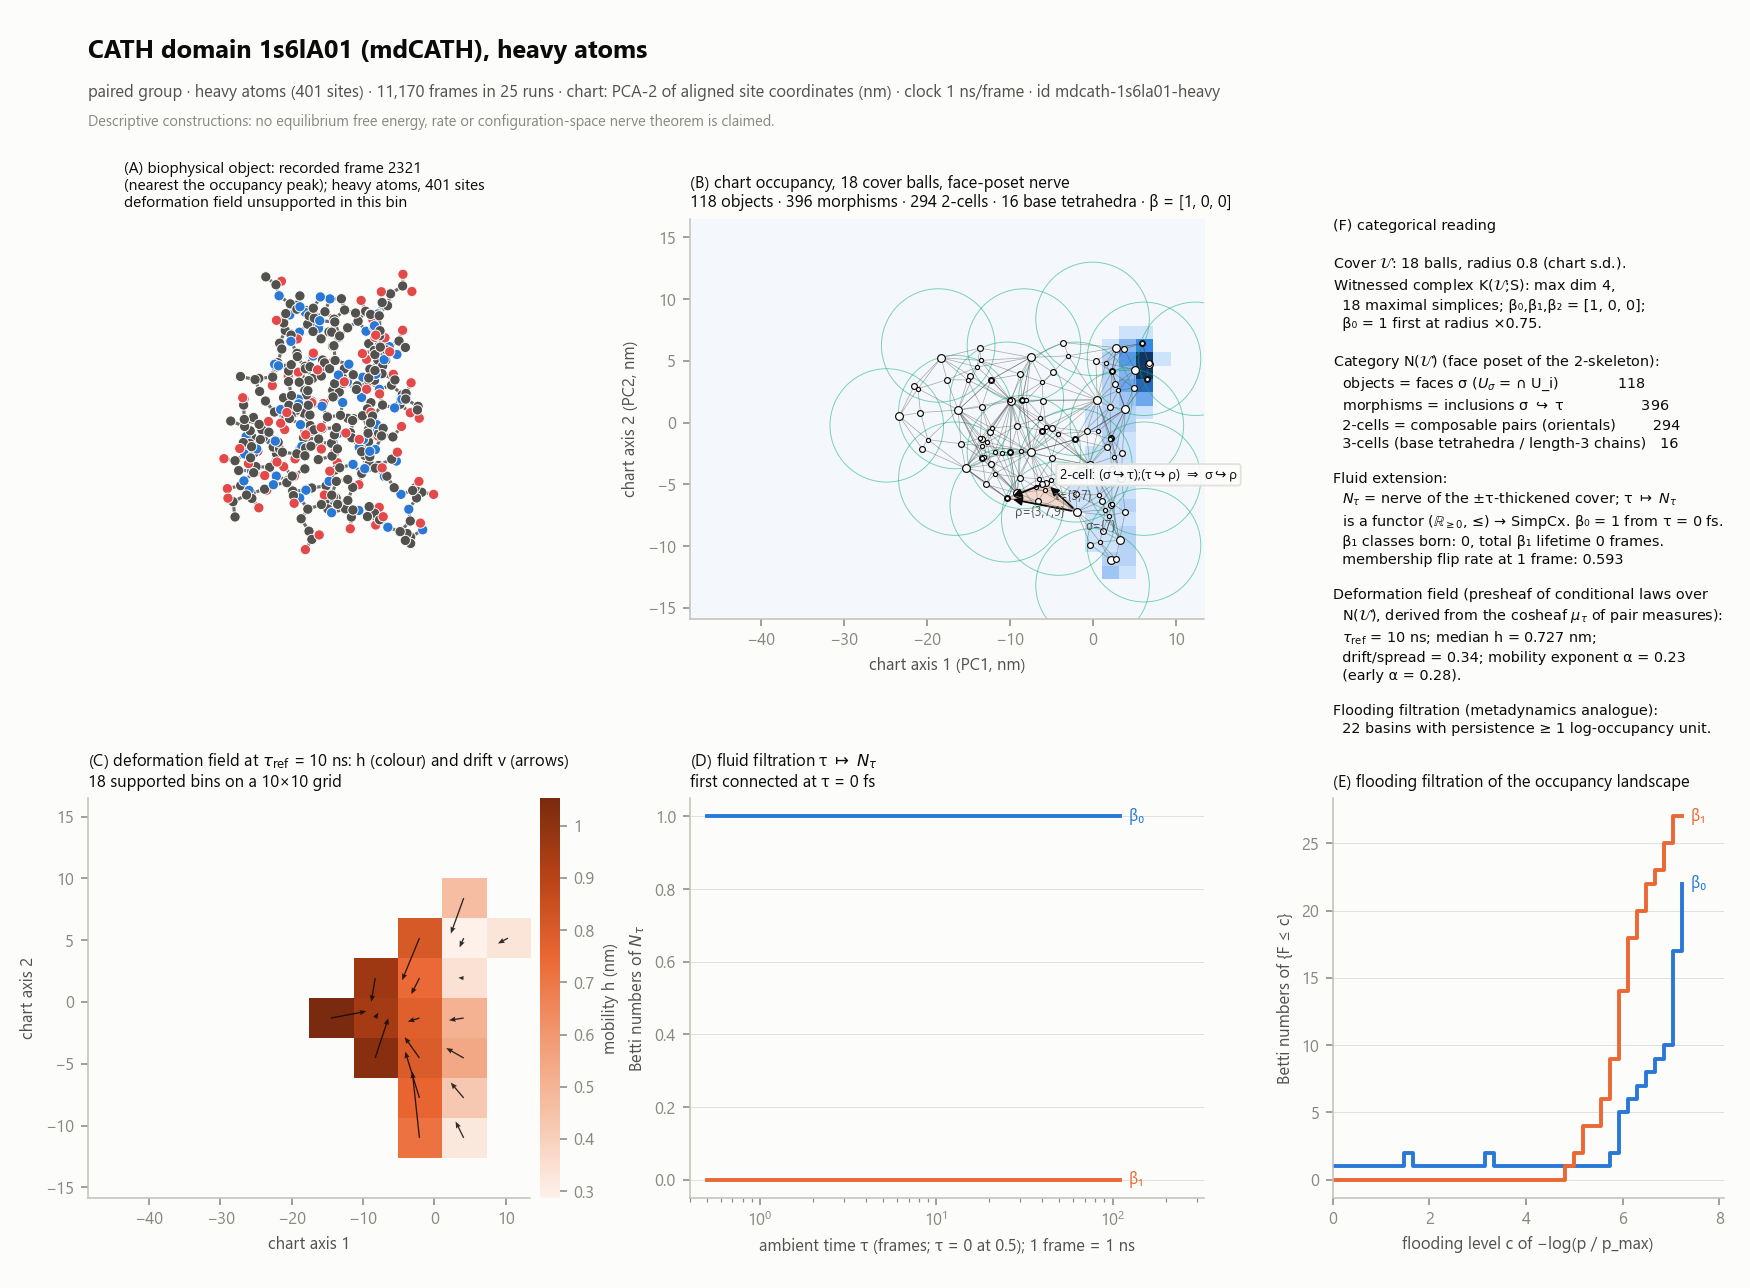
\includegraphics[width=\linewidth,height=.93\textheight,keepaspectratio]{systems/mdcath-1s6la01-heavy/plate.png}\caption{CATH domain 1s6lA01 (mdCATH), heavy atoms (\texttt{mdcath-1s6la01-heavy}), paired with \texttt{mdcath-1s6la01-ca}.}\end{figure}\clearpage
\begin{figure}[H]\centering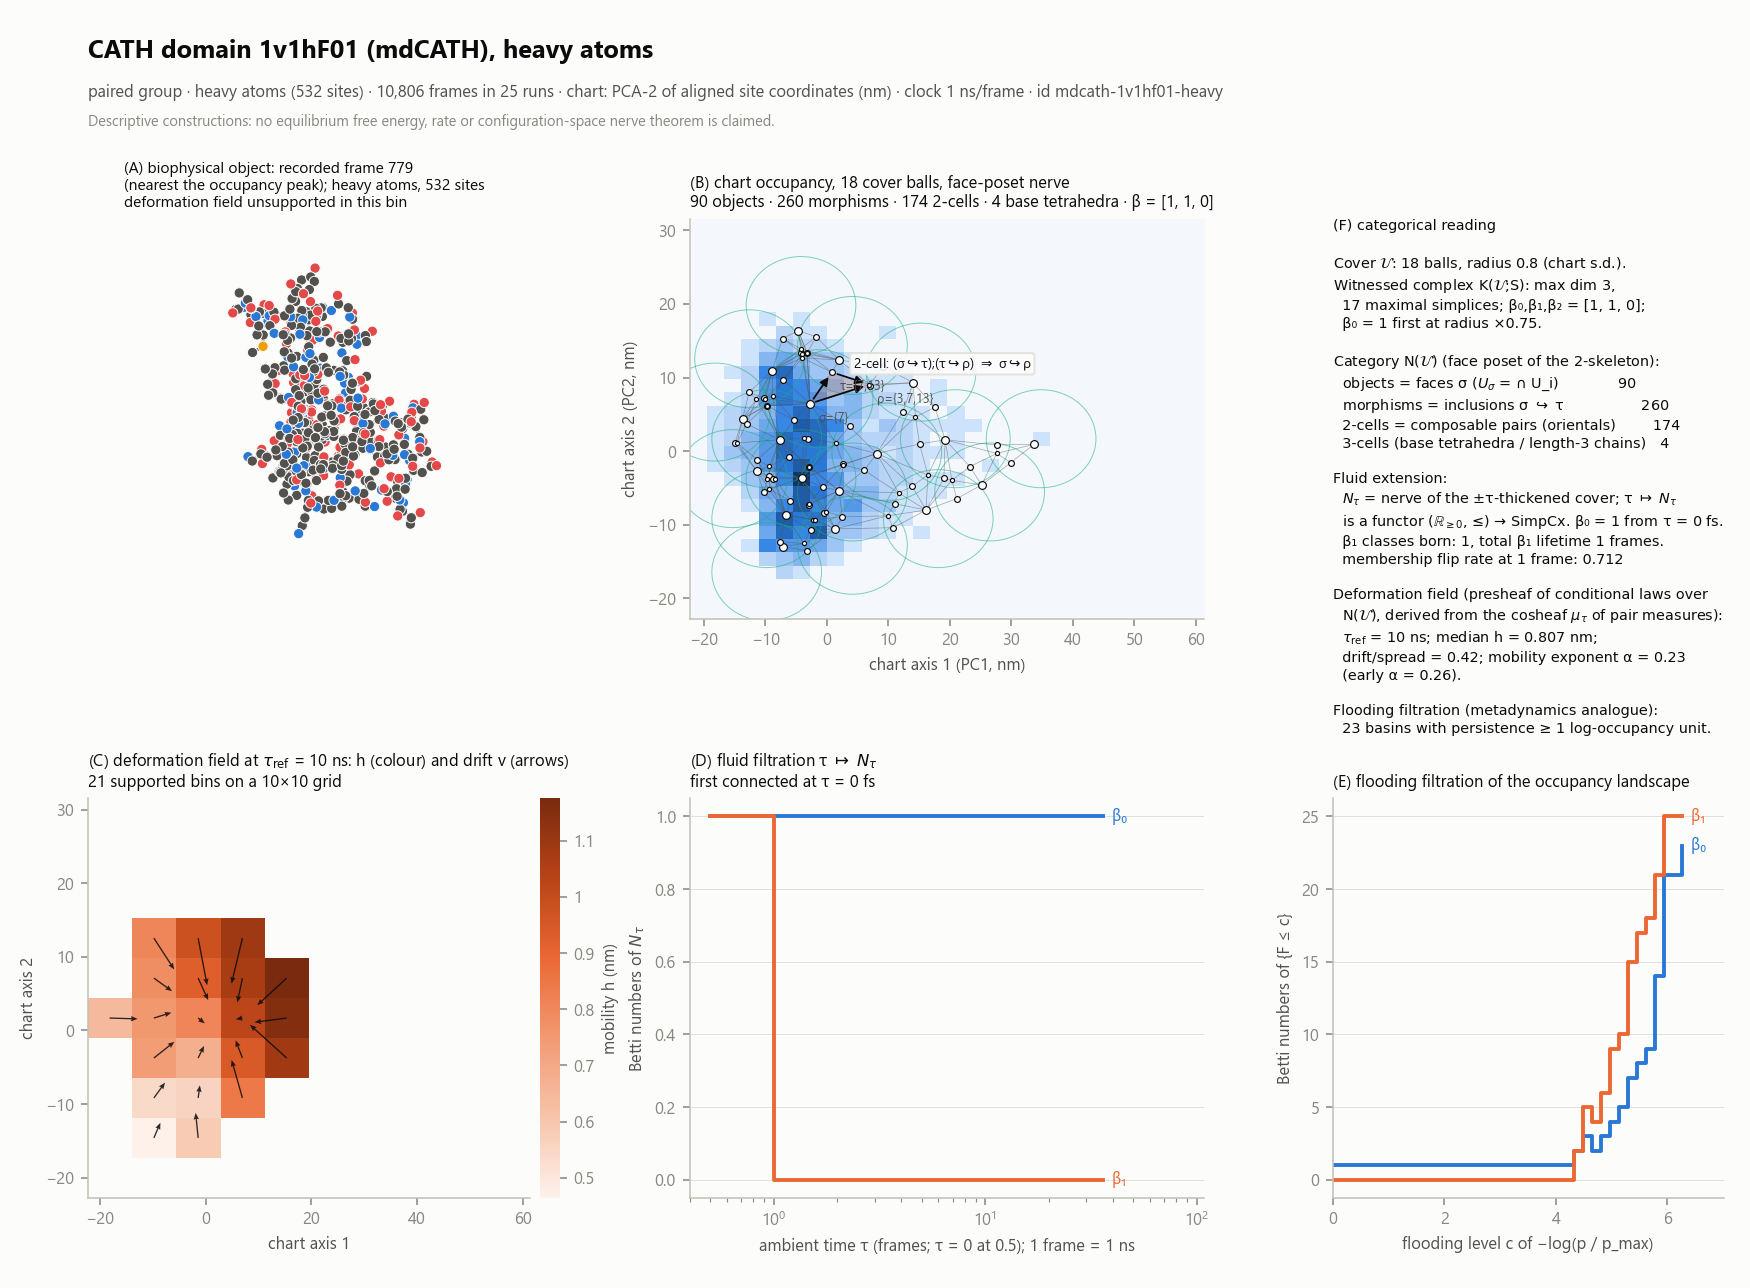
\includegraphics[width=\linewidth,height=.93\textheight,keepaspectratio]{systems/mdcath-1v1hf01-heavy/plate.png}\caption{CATH domain 1v1hF01 (mdCATH), heavy atoms (\texttt{mdcath-1v1hf01-heavy}), paired with \texttt{mdcath-1v1hf01-ca}.}\end{figure}\clearpage
\begin{figure}[H]\centering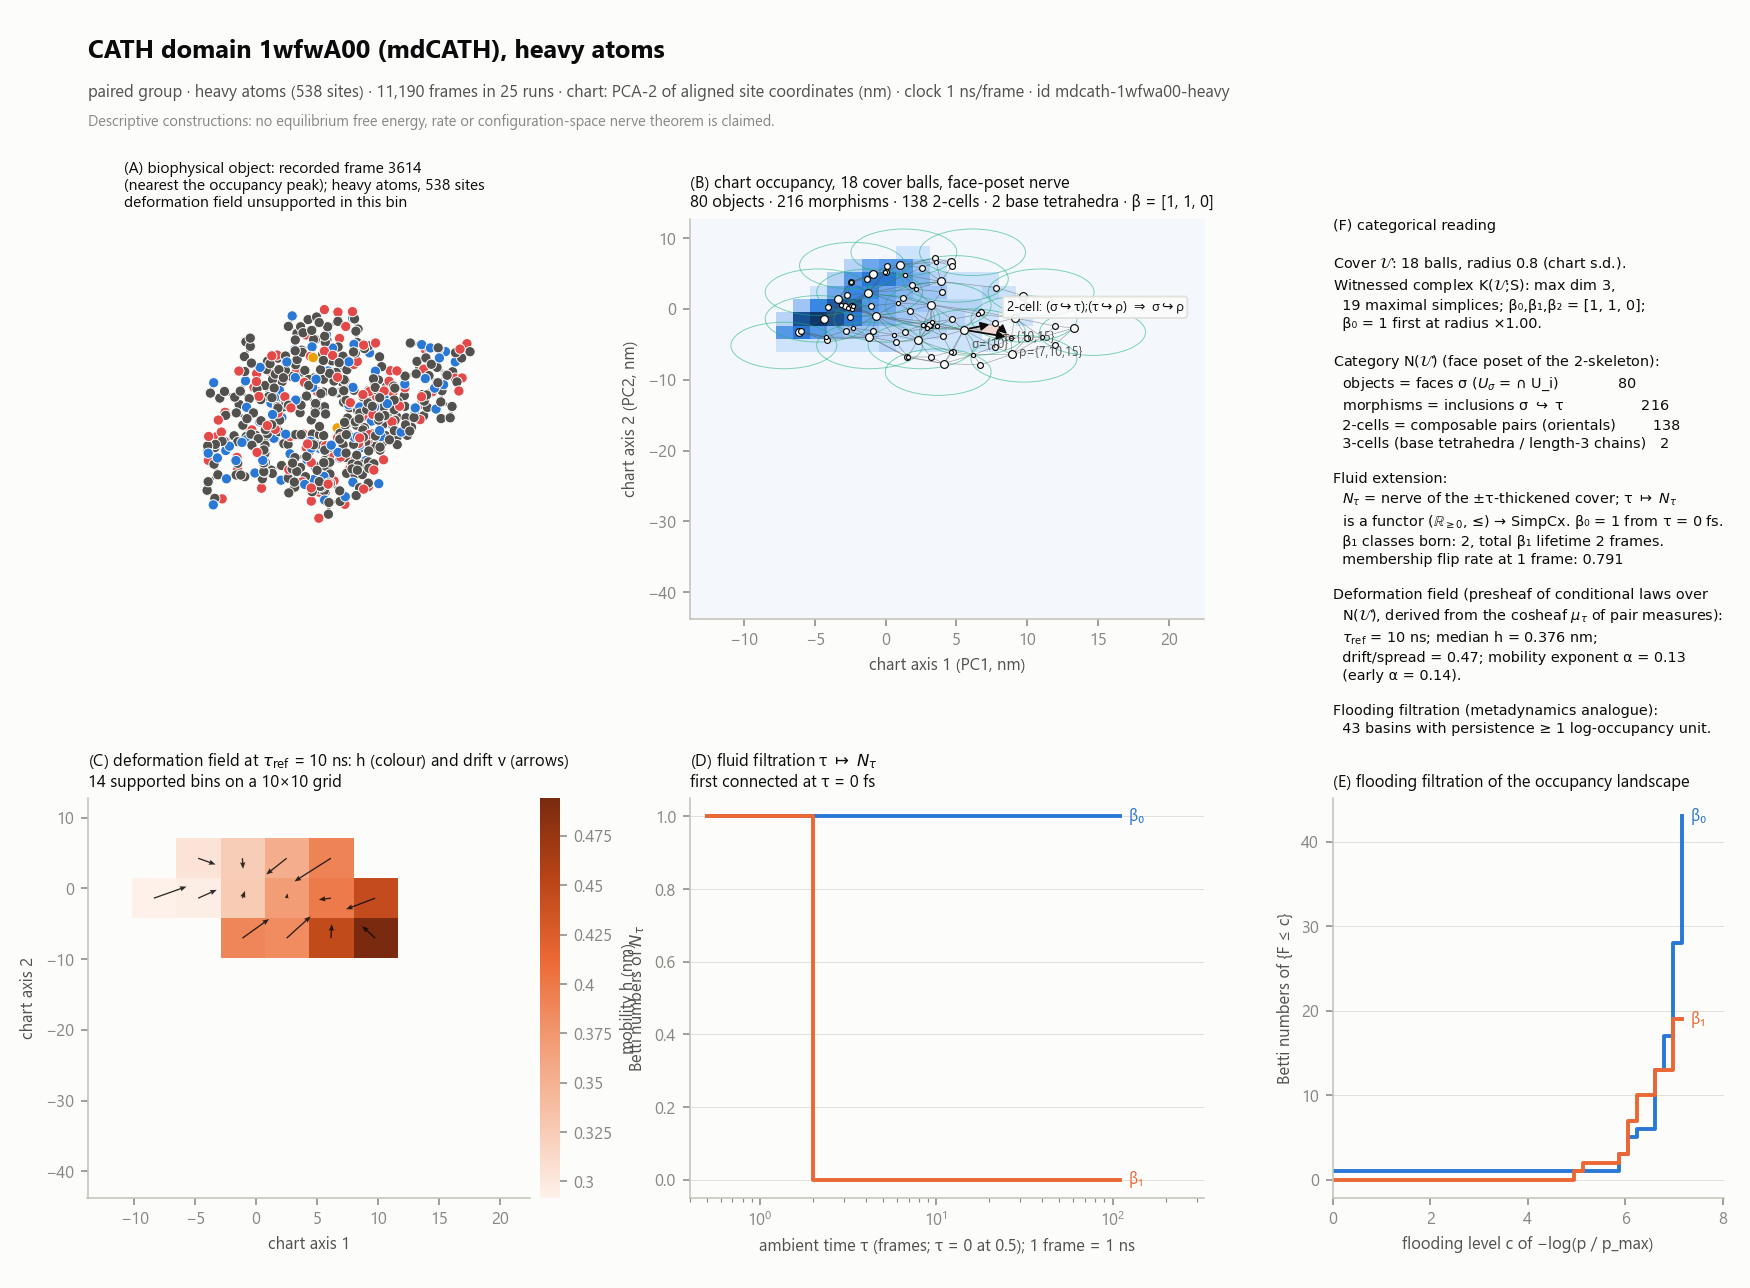
\includegraphics[width=\linewidth,height=.93\textheight,keepaspectratio]{systems/mdcath-1wfwa00-heavy/plate.png}\caption{CATH domain 1wfwA00 (mdCATH), heavy atoms (\texttt{mdcath-1wfwa00-heavy}), paired with \texttt{mdcath-1wfwa00-ca}.}\end{figure}\clearpage
\begin{figure}[H]\centering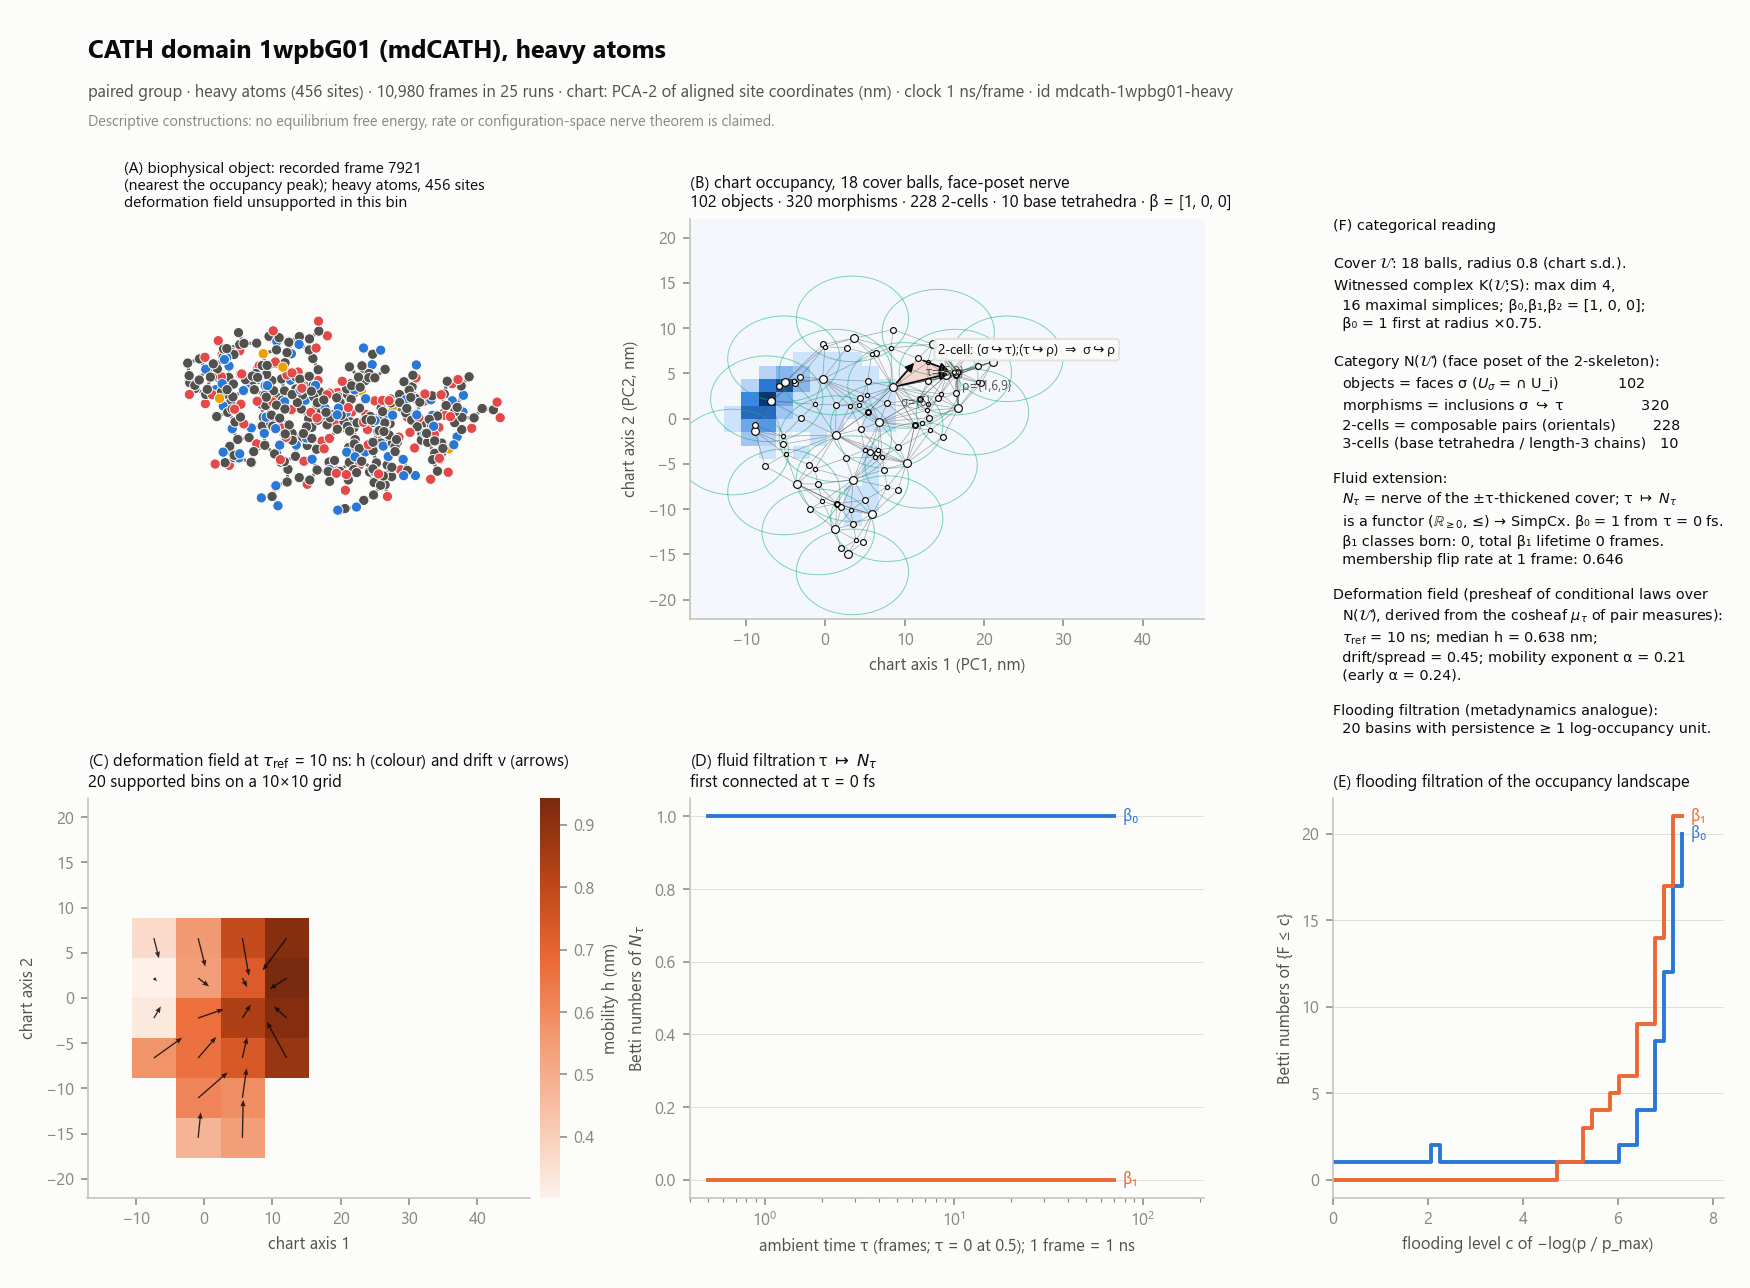
\includegraphics[width=\linewidth,height=.93\textheight,keepaspectratio]{systems/mdcath-1wpbg01-heavy/plate.png}\caption{CATH domain 1wpbG01 (mdCATH), heavy atoms (\texttt{mdcath-1wpbg01-heavy}), paired with \texttt{mdcath-1wpbg01-ca}.}\end{figure}\clearpage
\begin{figure}[H]\centering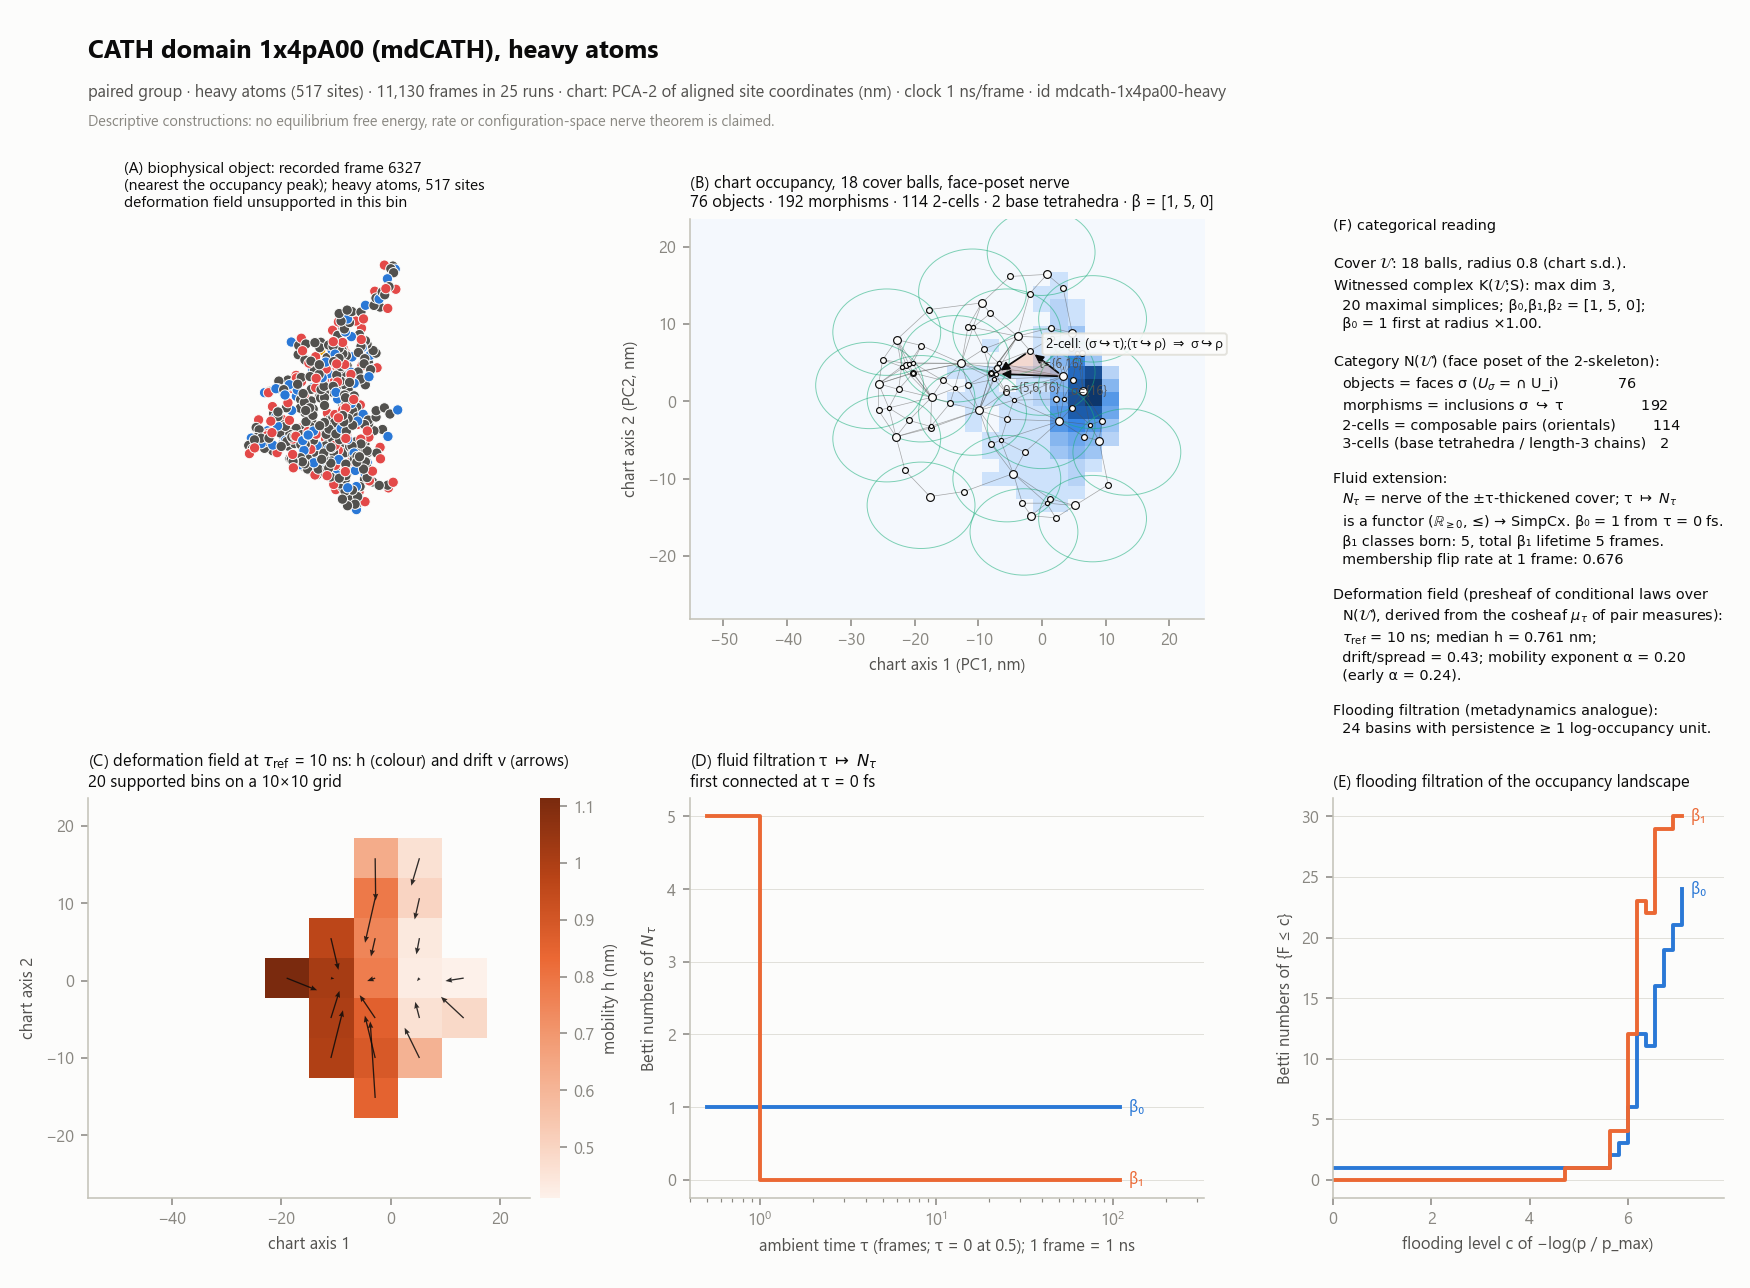
\includegraphics[width=\linewidth,height=.93\textheight,keepaspectratio]{systems/mdcath-1x4pa00-heavy/plate.png}\caption{CATH domain 1x4pA00 (mdCATH), heavy atoms (\texttt{mdcath-1x4pa00-heavy}), paired with \texttt{mdcath-1x4pa00-ca}.}\end{figure}\clearpage
\begin{figure}[H]\centering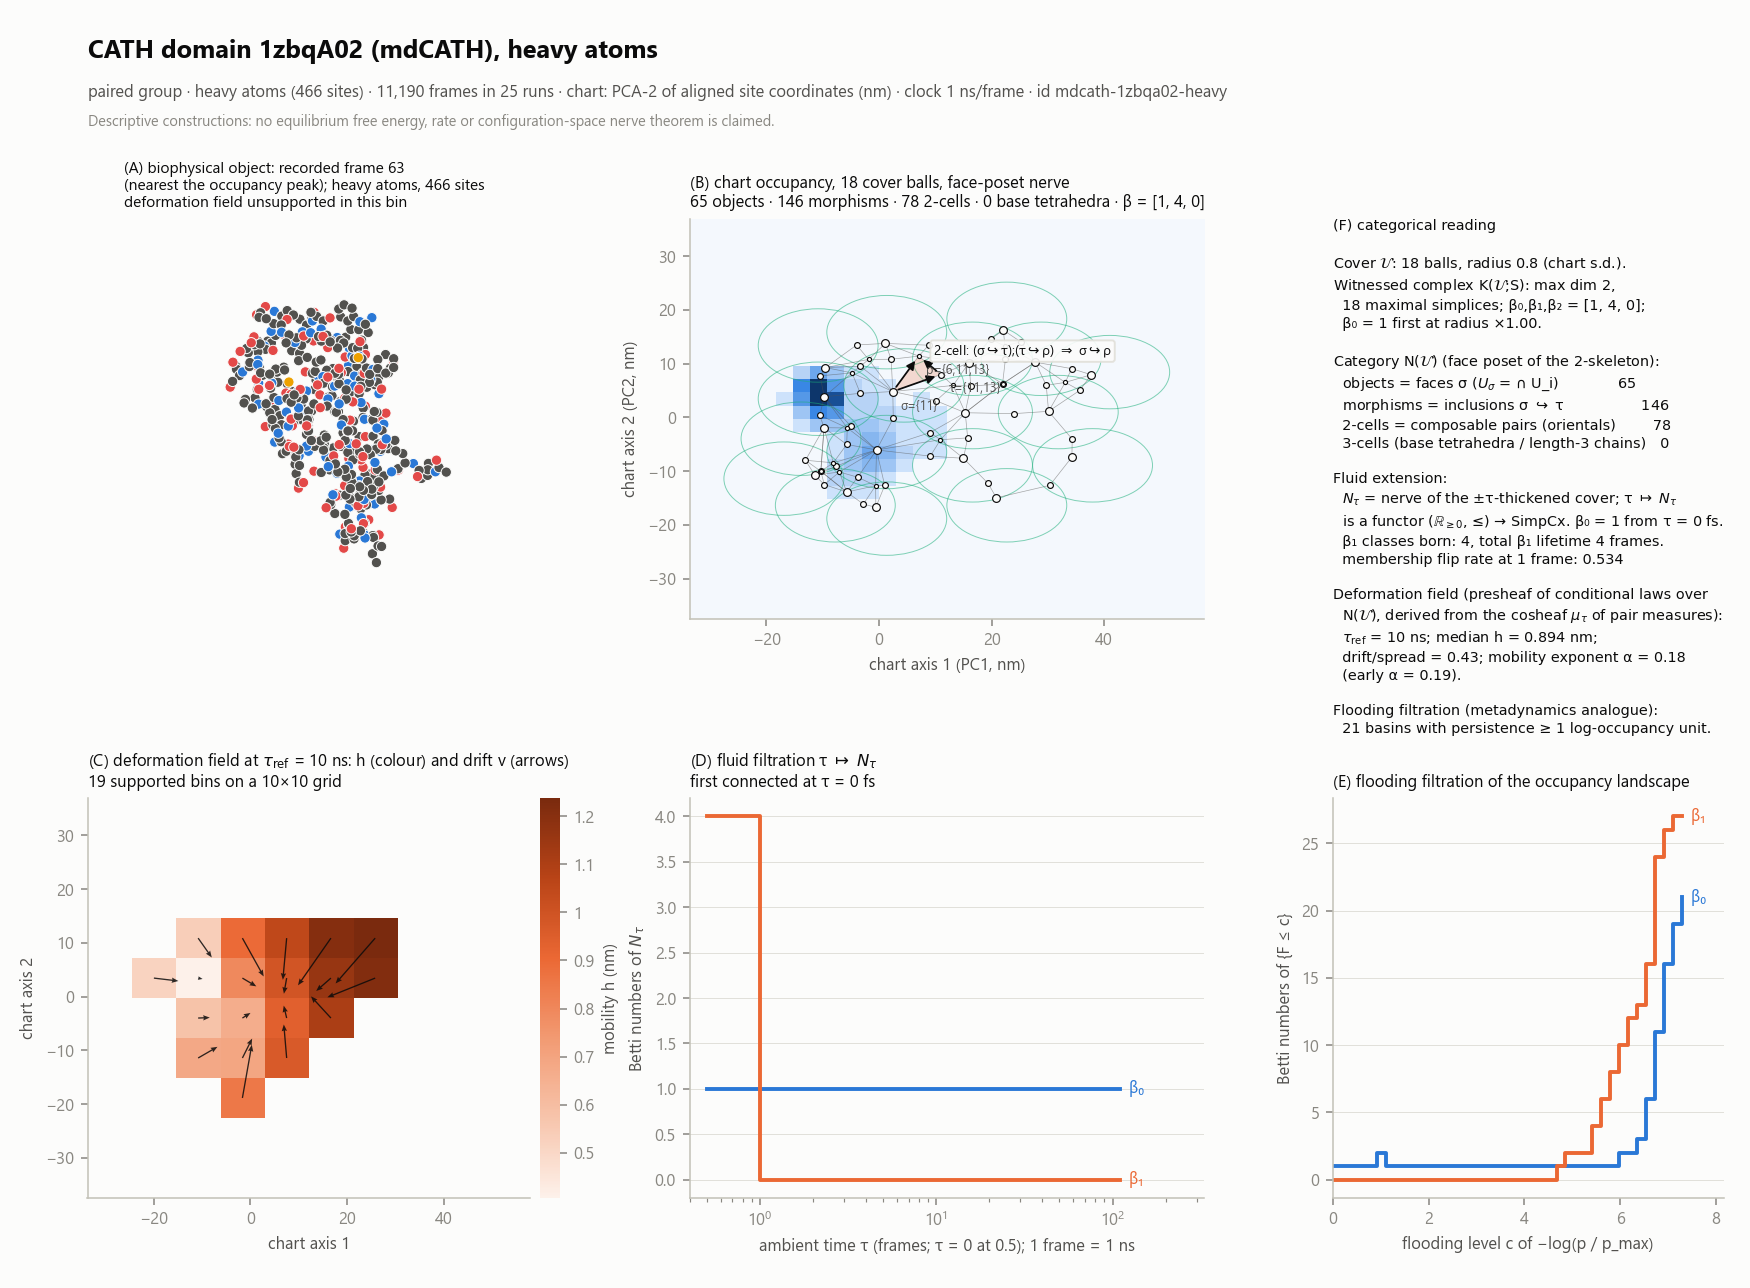
\includegraphics[width=\linewidth,height=.93\textheight,keepaspectratio]{systems/mdcath-1zbqa02-heavy/plate.png}\caption{CATH domain 1zbqA02 (mdCATH), heavy atoms (\texttt{mdcath-1zbqa02-heavy}), paired with \texttt{mdcath-1zbqa02-ca}.}\end{figure}\clearpage
\begin{figure}[H]\centering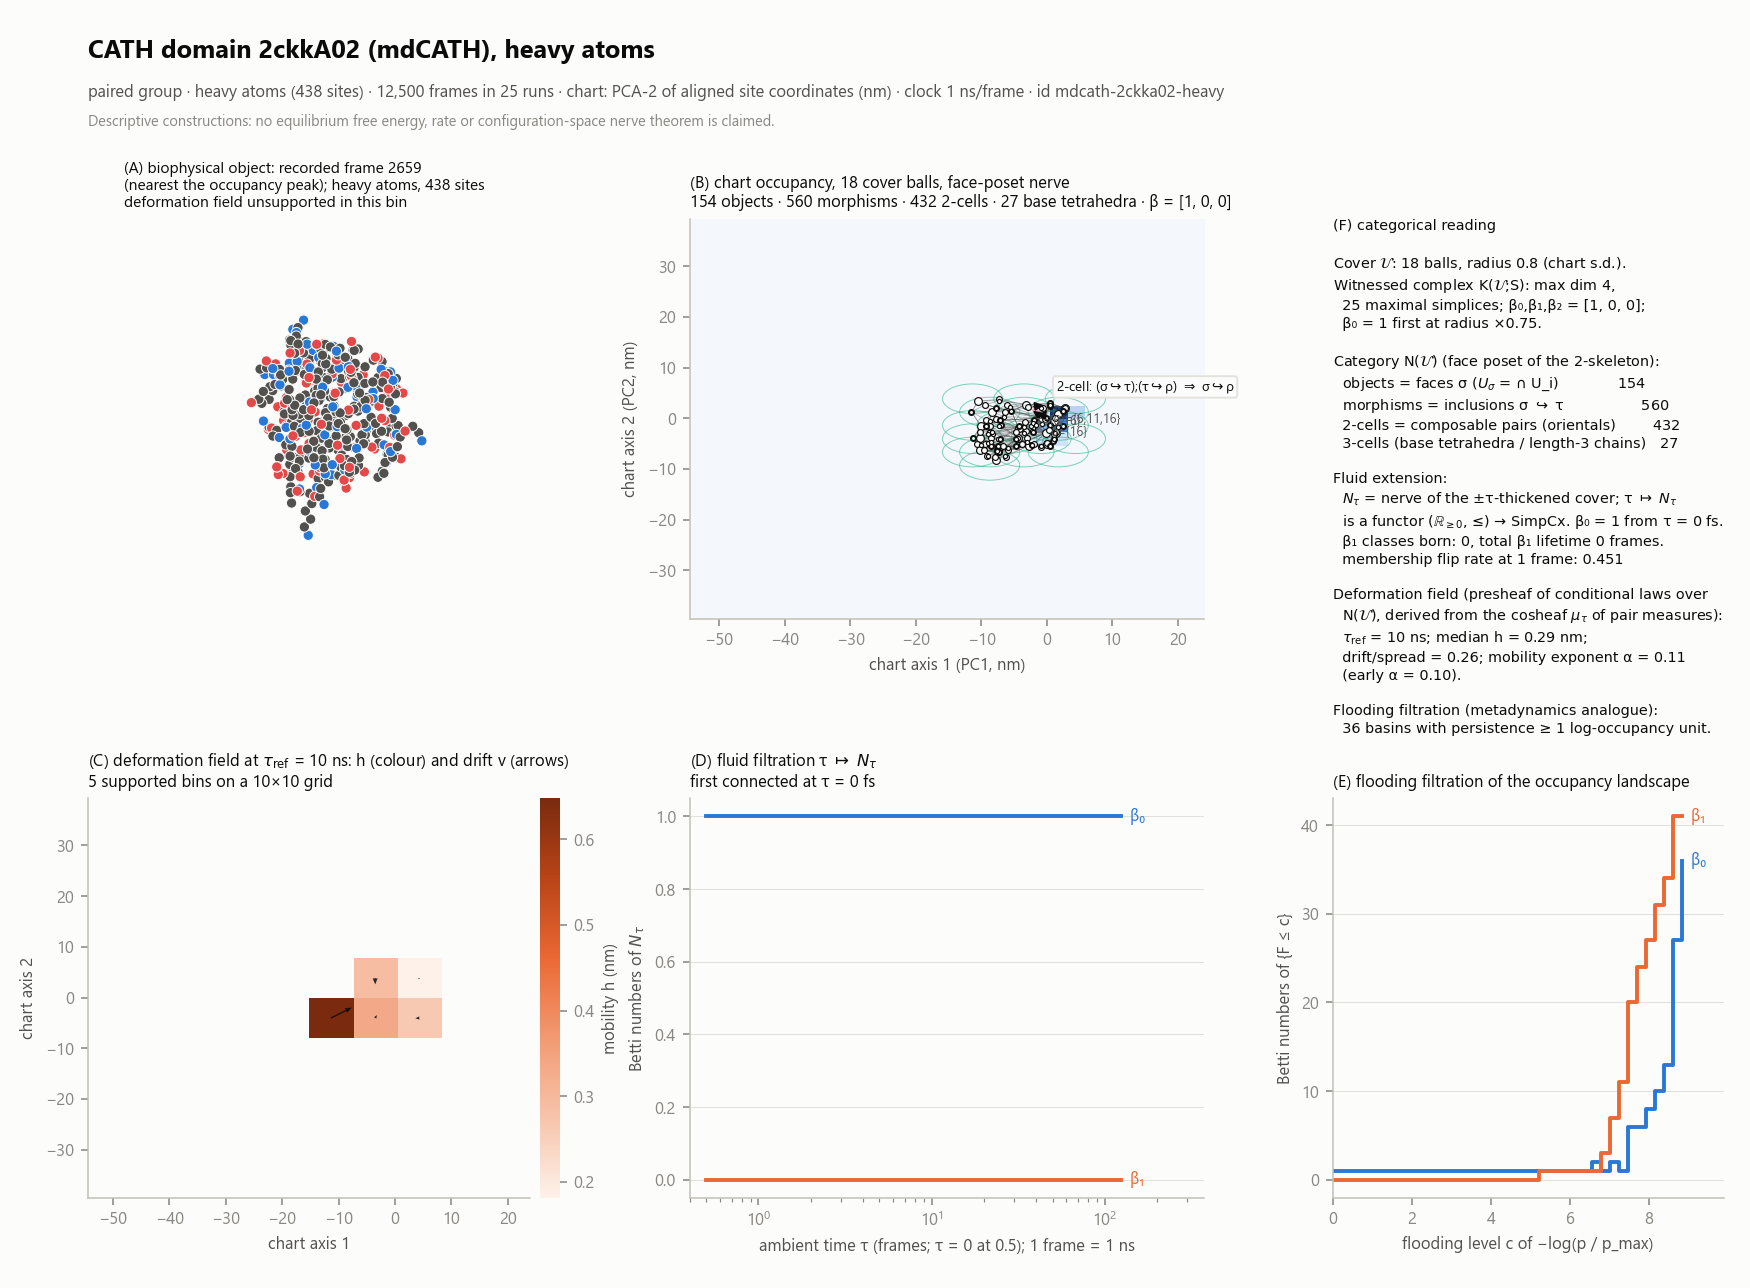
\includegraphics[width=\linewidth,height=.93\textheight,keepaspectratio]{systems/mdcath-2ckka02-heavy/plate.png}\caption{CATH domain 2ckkA02 (mdCATH), heavy atoms (\texttt{mdcath-2ckka02-heavy}), paired with \texttt{mdcath-2ckka02-ca}.}\end{figure}\clearpage
\begin{figure}[H]\centering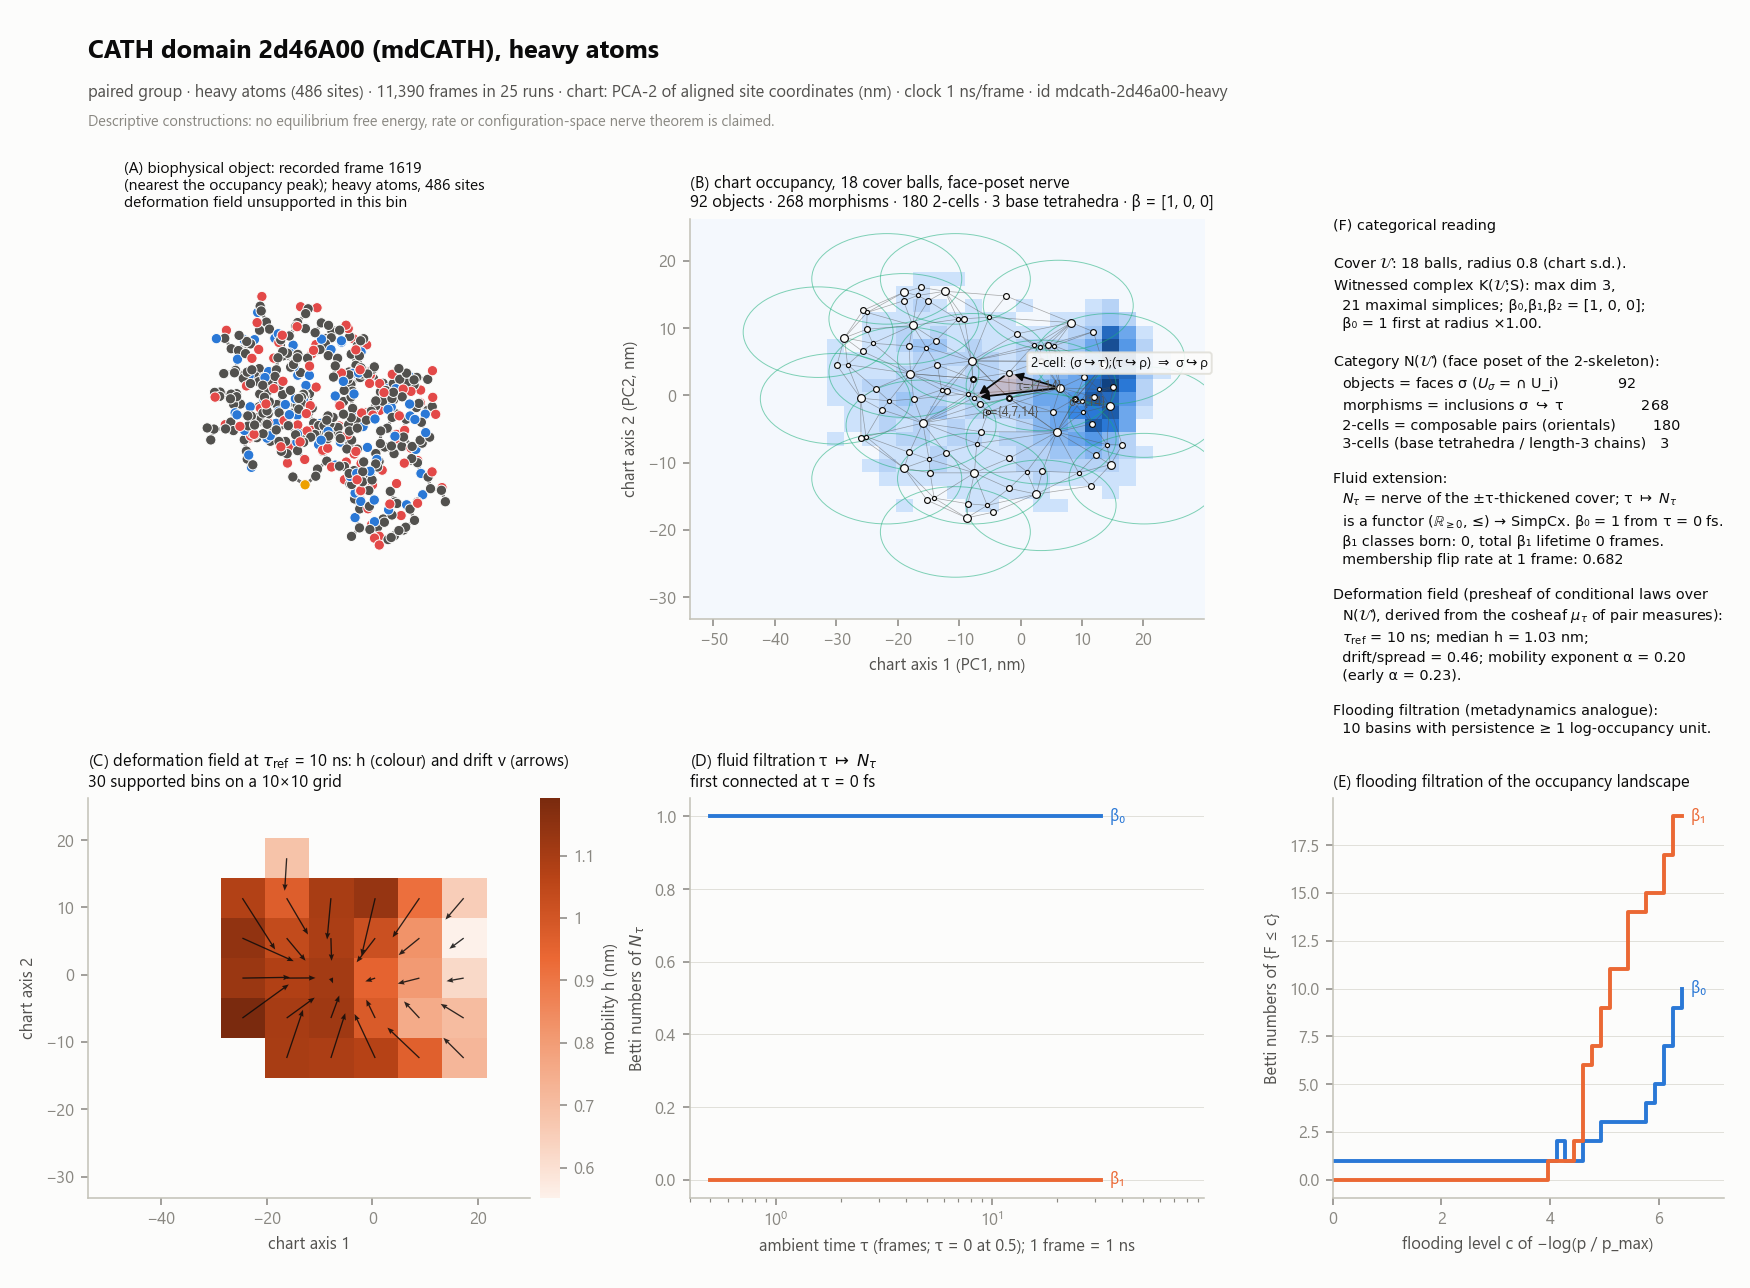
\includegraphics[width=\linewidth,height=.93\textheight,keepaspectratio]{systems/mdcath-2d46a00-heavy/plate.png}\caption{CATH domain 2d46A00 (mdCATH), heavy atoms (\texttt{mdcath-2d46a00-heavy}), paired with \texttt{mdcath-2d46a00-ca}.}\end{figure}\clearpage
\begin{figure}[H]\centering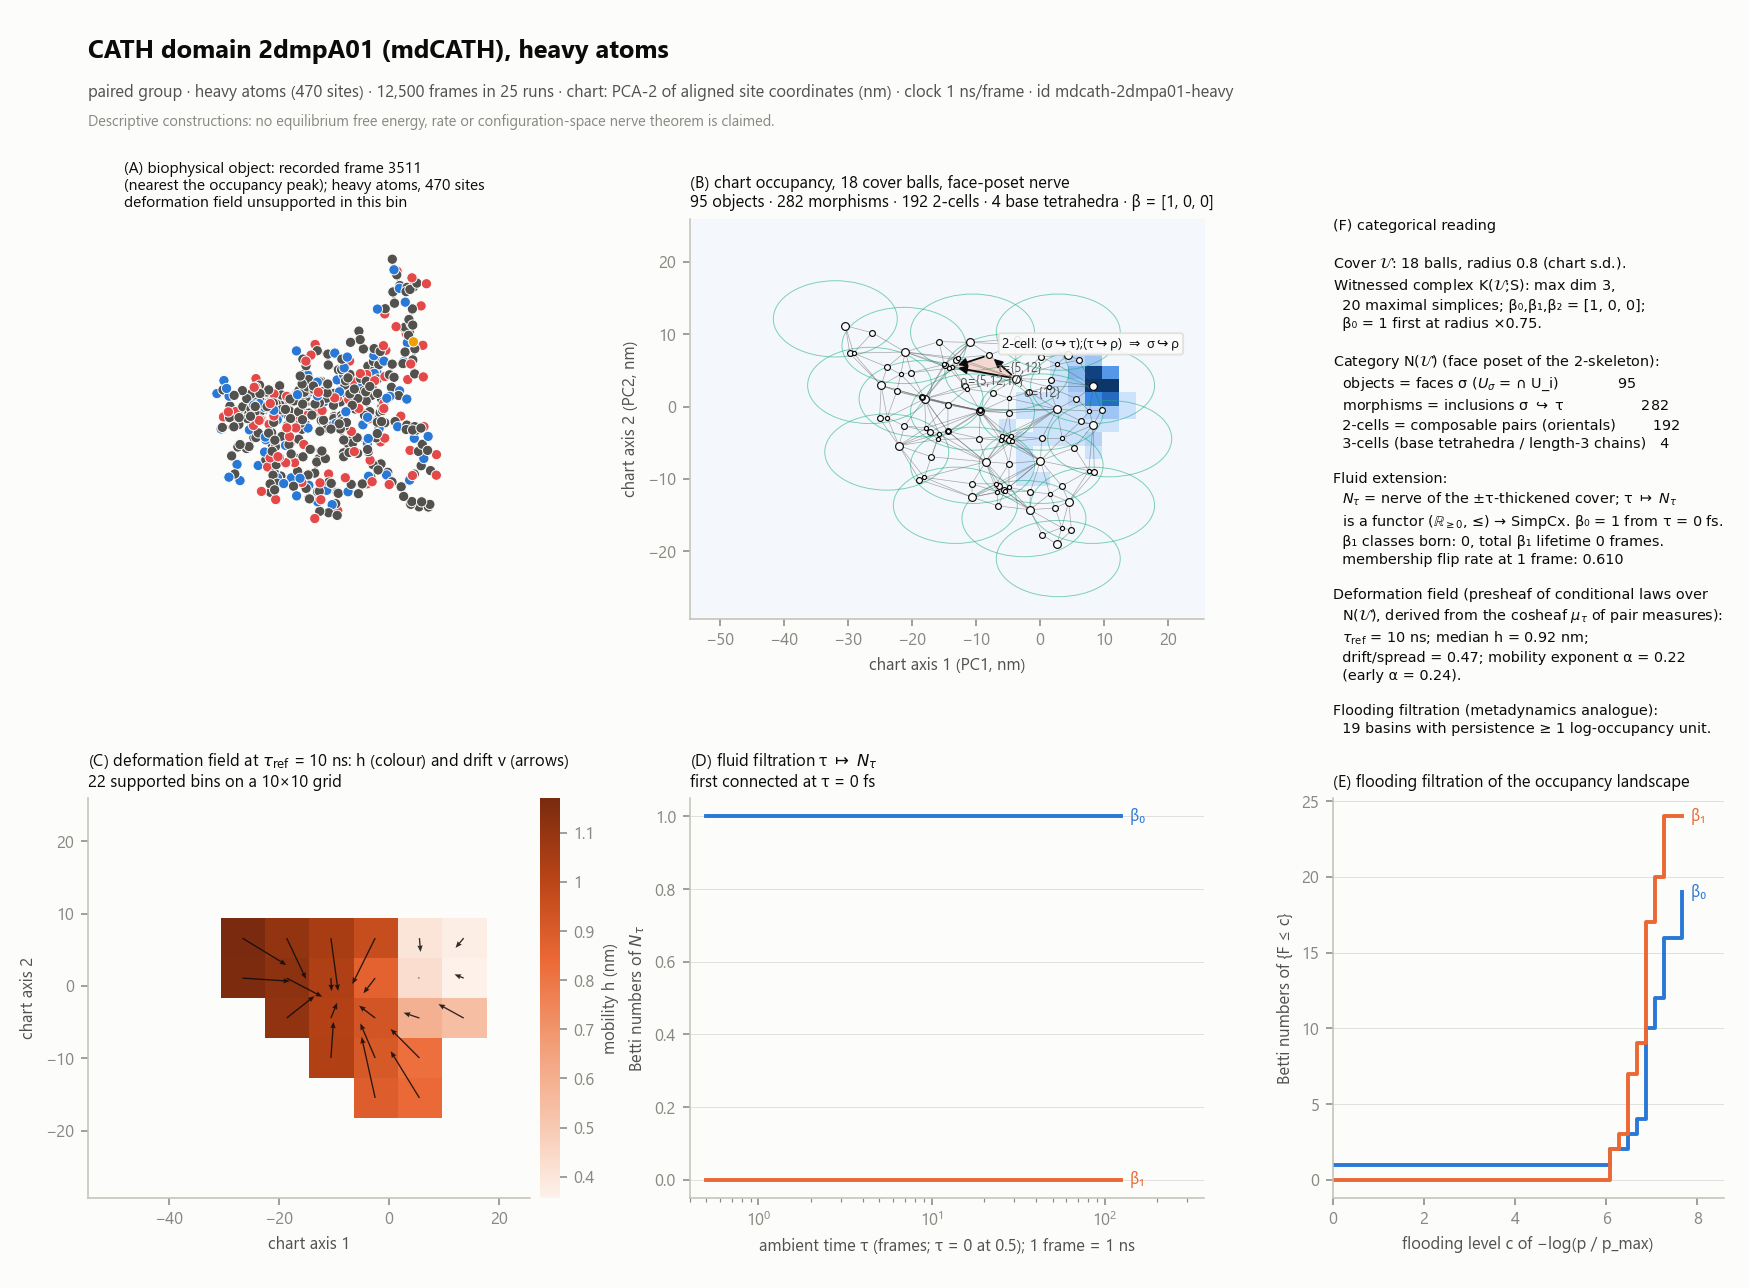
\includegraphics[width=\linewidth,height=.93\textheight,keepaspectratio]{systems/mdcath-2dmpa01-heavy/plate.png}\caption{CATH domain 2dmpA01 (mdCATH), heavy atoms (\texttt{mdcath-2dmpa01-heavy}), paired with \texttt{mdcath-2dmpa01-ca}.}\end{figure}\clearpage
\begin{figure}[H]\centering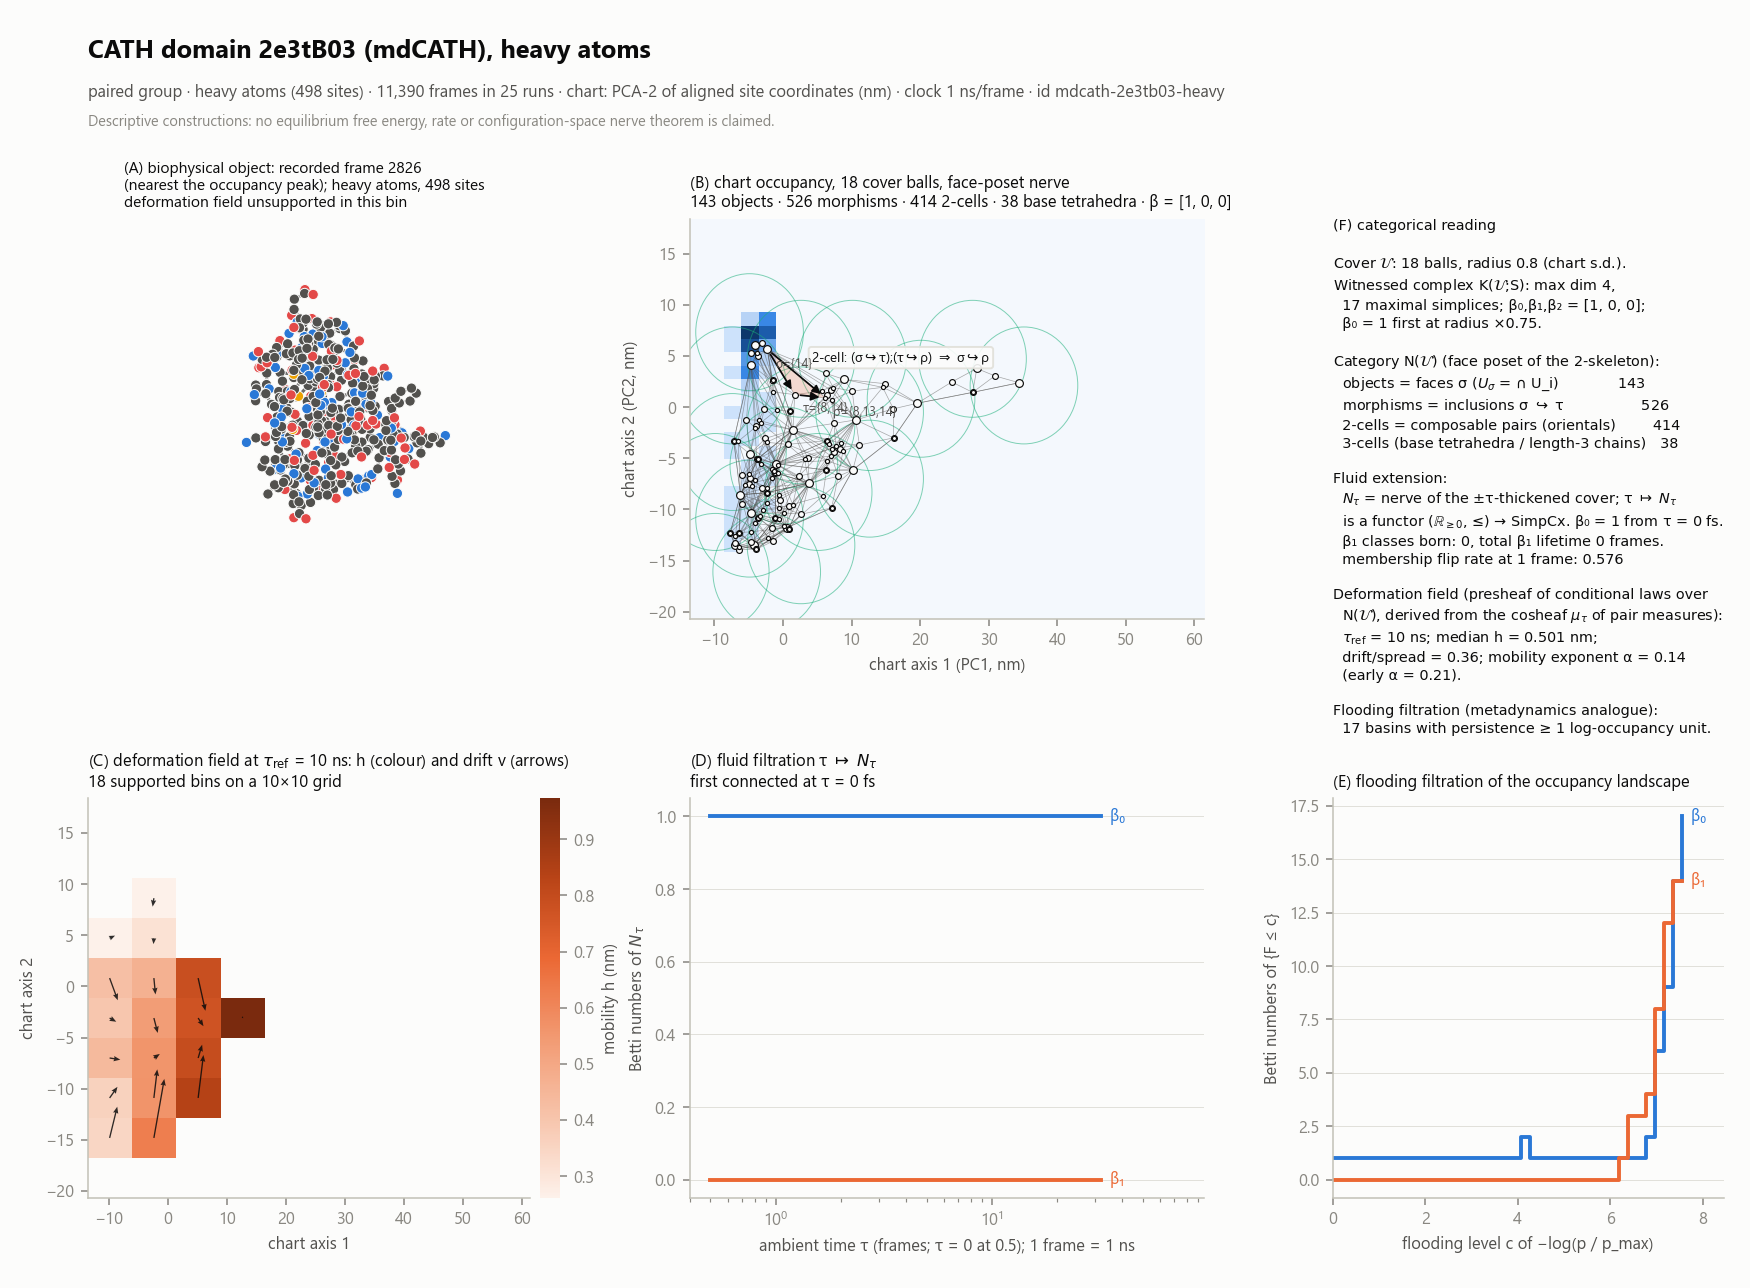
\includegraphics[width=\linewidth,height=.93\textheight,keepaspectratio]{systems/mdcath-2e3tb03-heavy/plate.png}\caption{CATH domain 2e3tB03 (mdCATH), heavy atoms (\texttt{mdcath-2e3tb03-heavy}), paired with \texttt{mdcath-2e3tb03-ca}.}\end{figure}\clearpage
\begin{figure}[H]\centering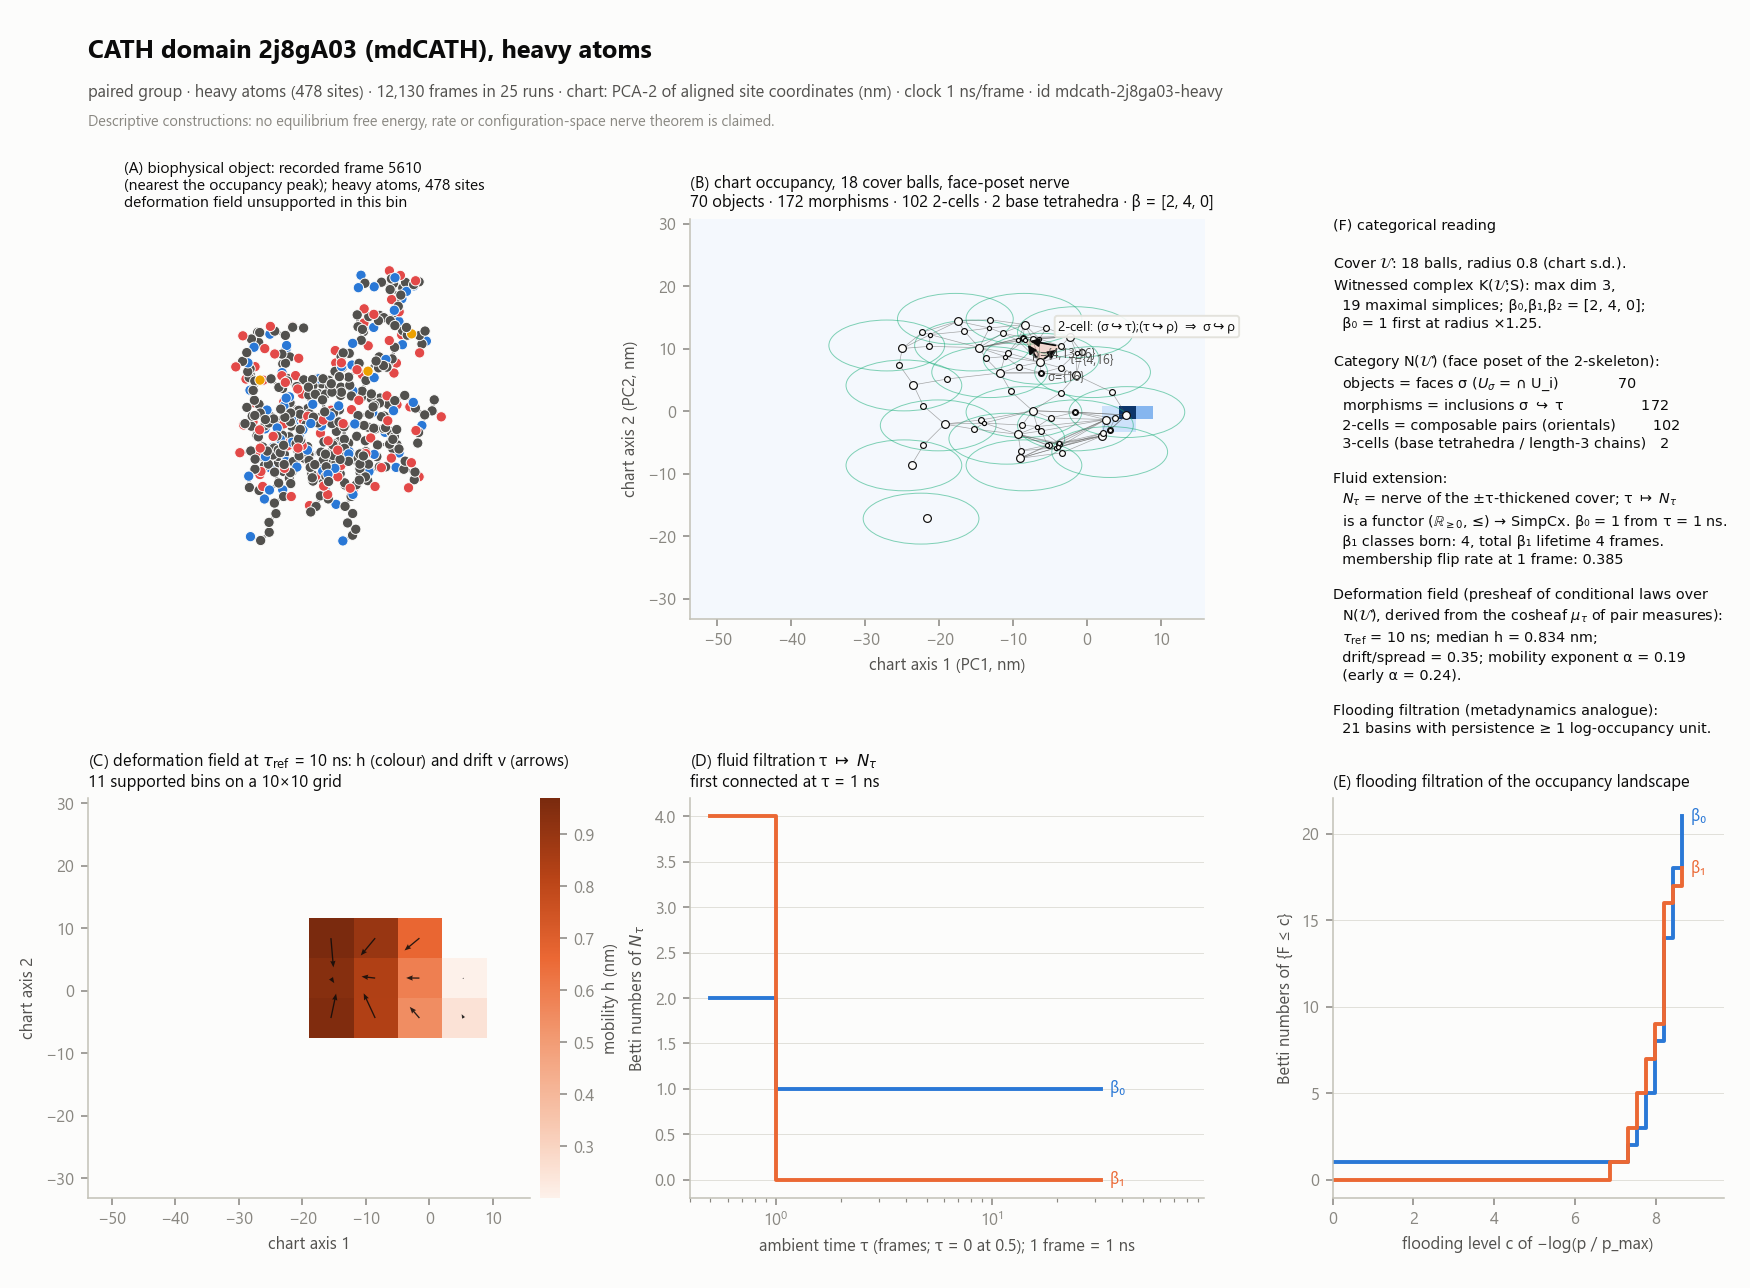
\includegraphics[width=\linewidth,height=.93\textheight,keepaspectratio]{systems/mdcath-2j8ga03-heavy/plate.png}\caption{CATH domain 2j8gA03 (mdCATH), heavy atoms (\texttt{mdcath-2j8ga03-heavy}), paired with \texttt{mdcath-2j8ga03-ca}.}\end{figure}\clearpage
\begin{figure}[H]\centering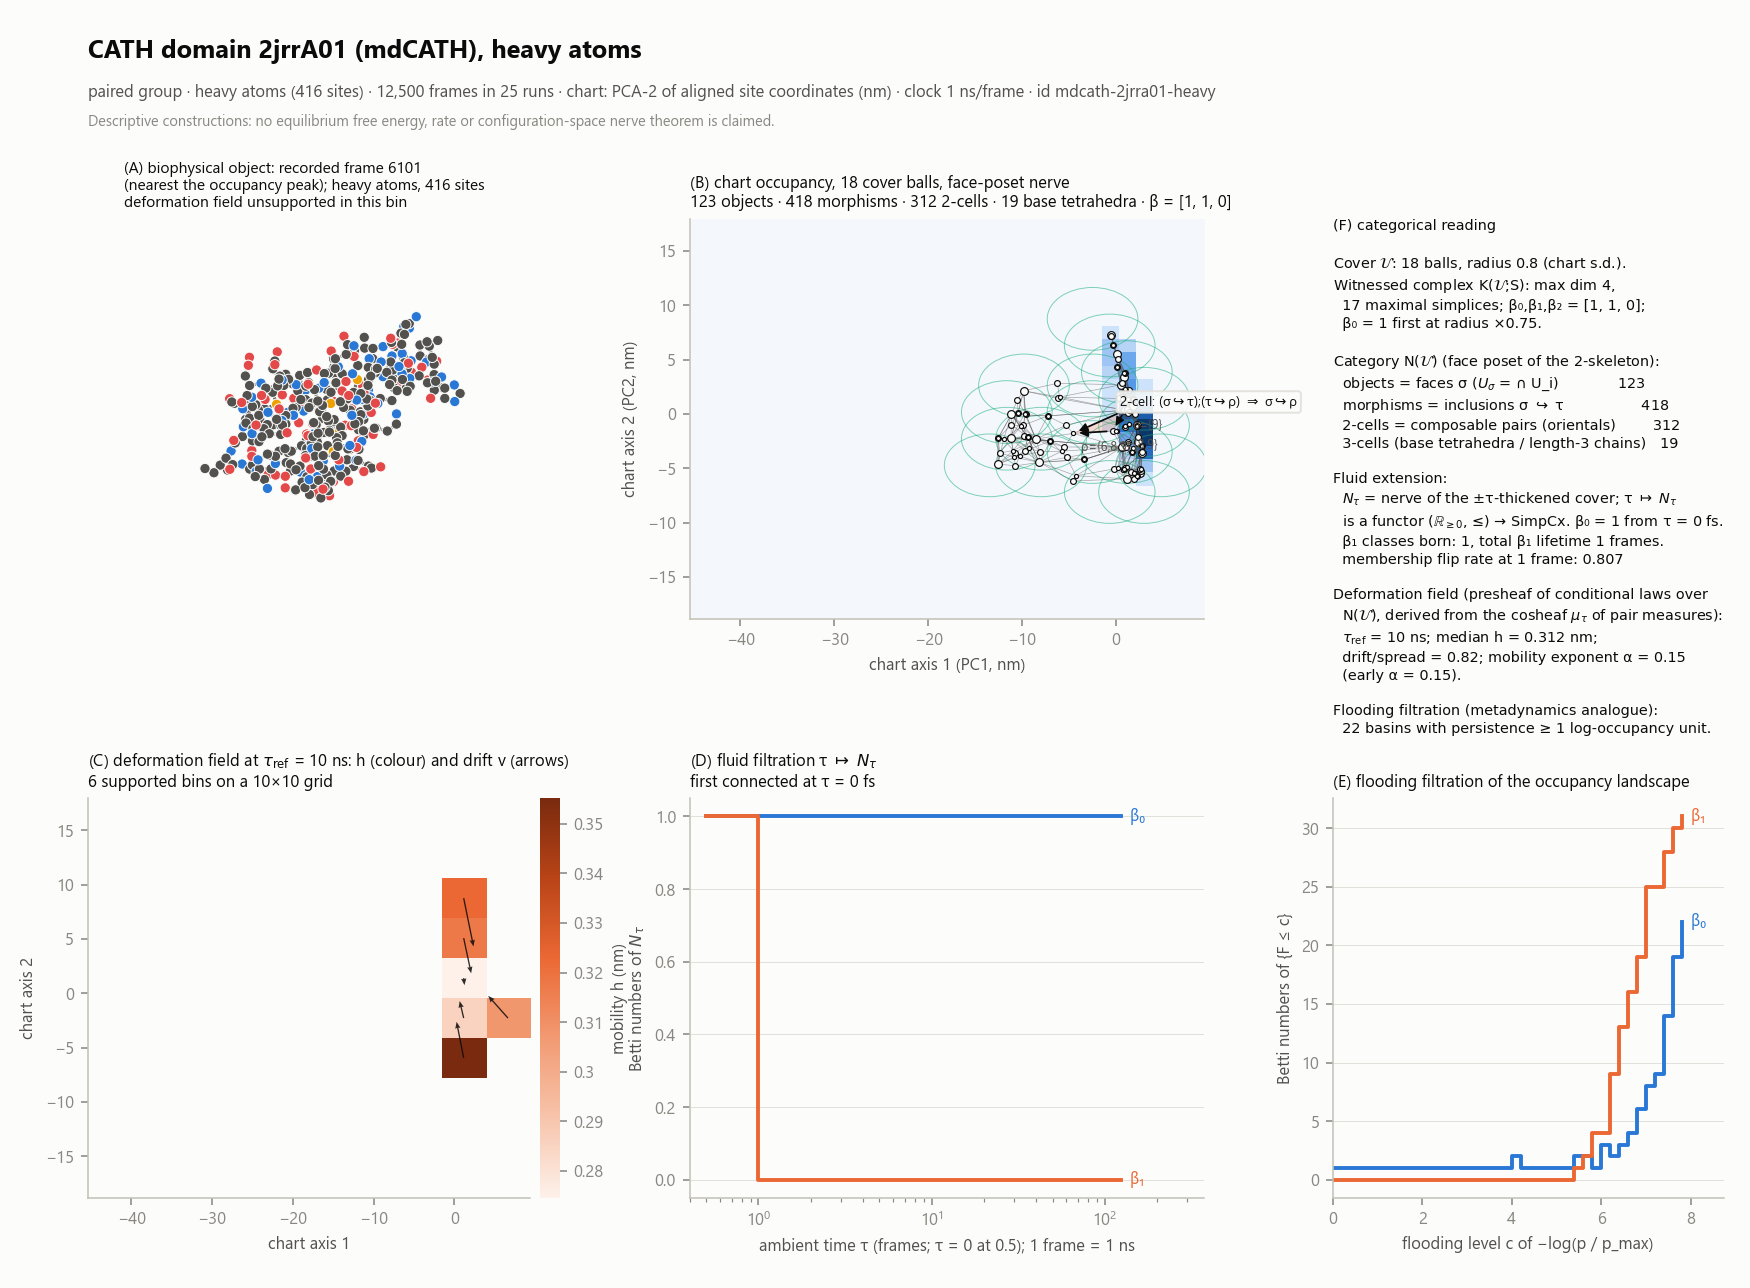
\includegraphics[width=\linewidth,height=.93\textheight,keepaspectratio]{systems/mdcath-2jrra01-heavy/plate.png}\caption{CATH domain 2jrrA01 (mdCATH), heavy atoms (\texttt{mdcath-2jrra01-heavy}), paired with \texttt{mdcath-2jrra01-ca}.}\end{figure}\clearpage
\begin{figure}[H]\centering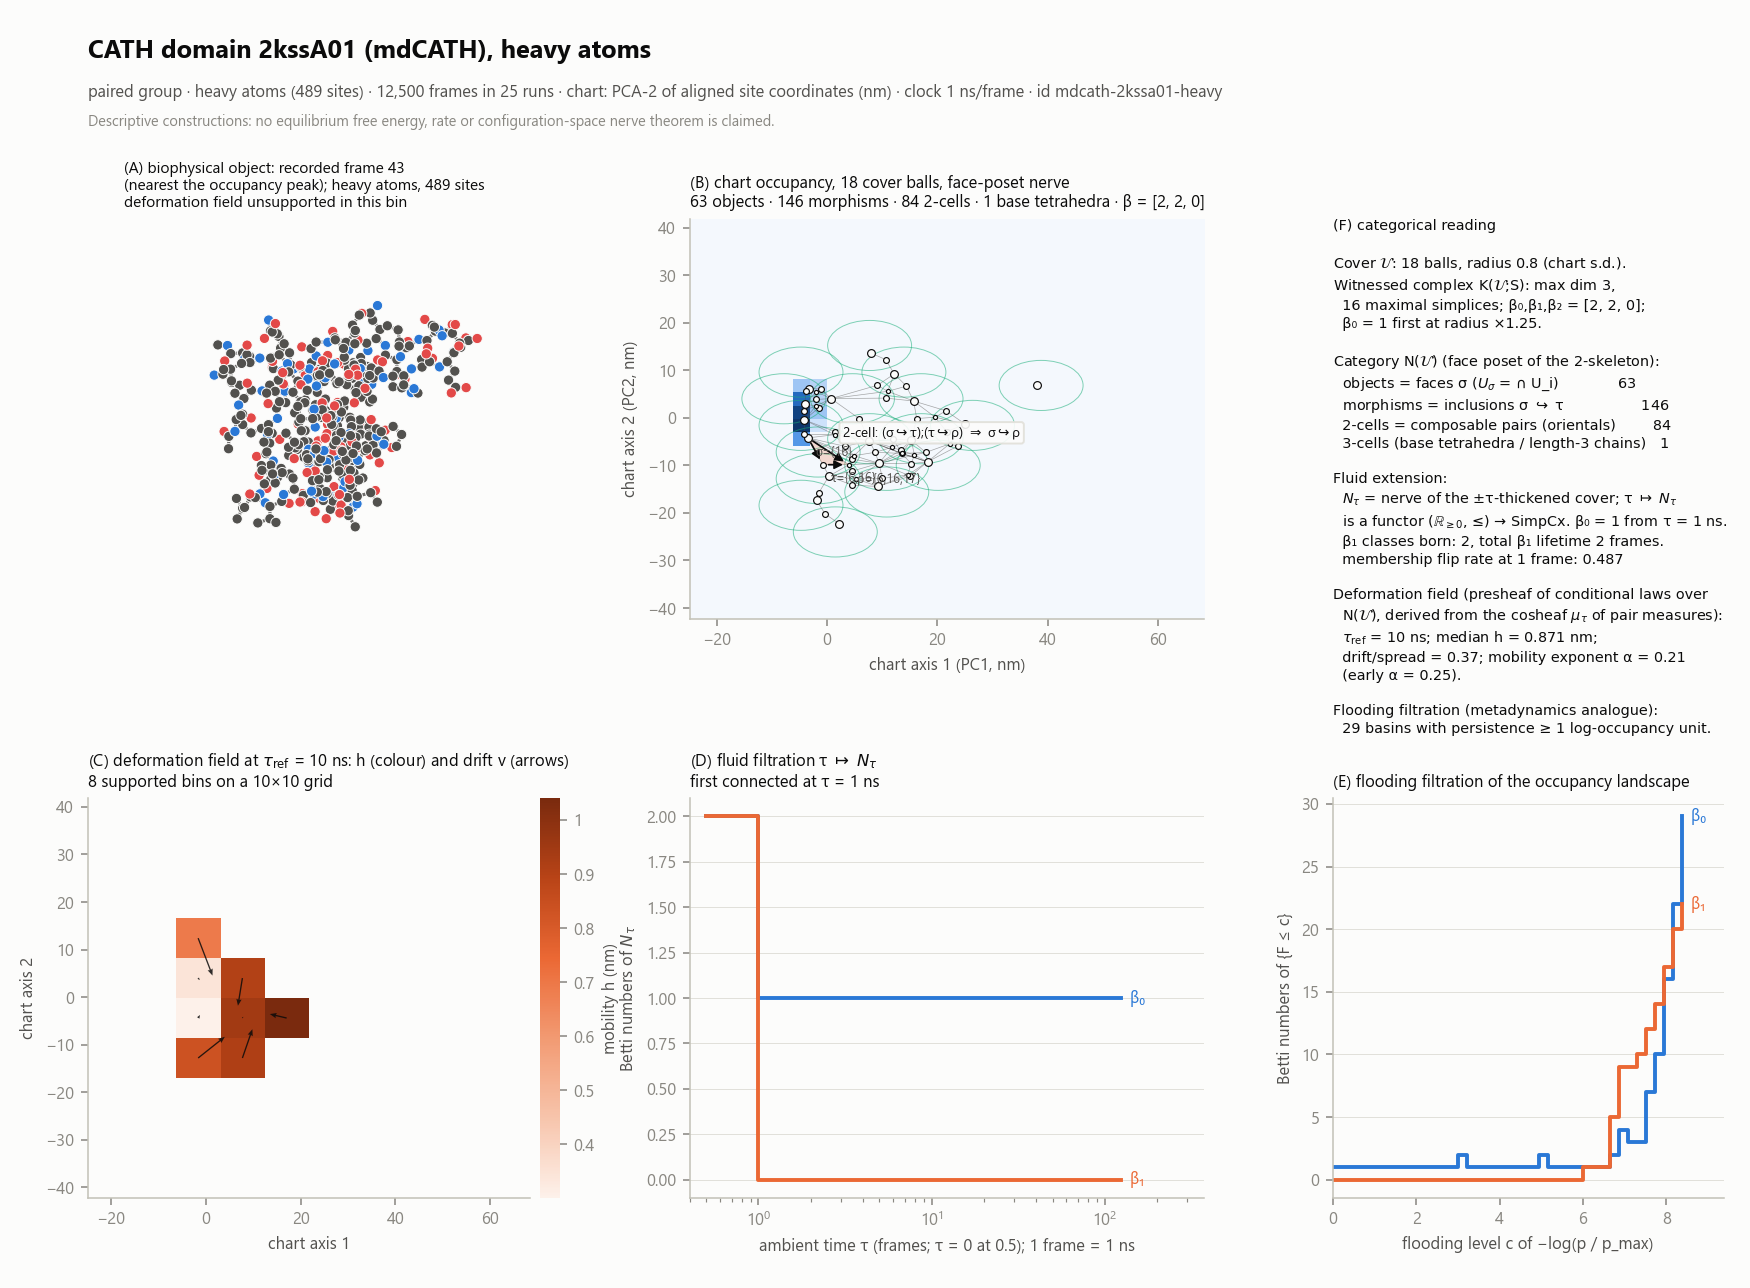
\includegraphics[width=\linewidth,height=.93\textheight,keepaspectratio]{systems/mdcath-2kssa01-heavy/plate.png}\caption{CATH domain 2kssA01 (mdCATH), heavy atoms (\texttt{mdcath-2kssa01-heavy}), paired with \texttt{mdcath-2kssa01-ca}.}\end{figure}\clearpage
\begin{figure}[H]\centering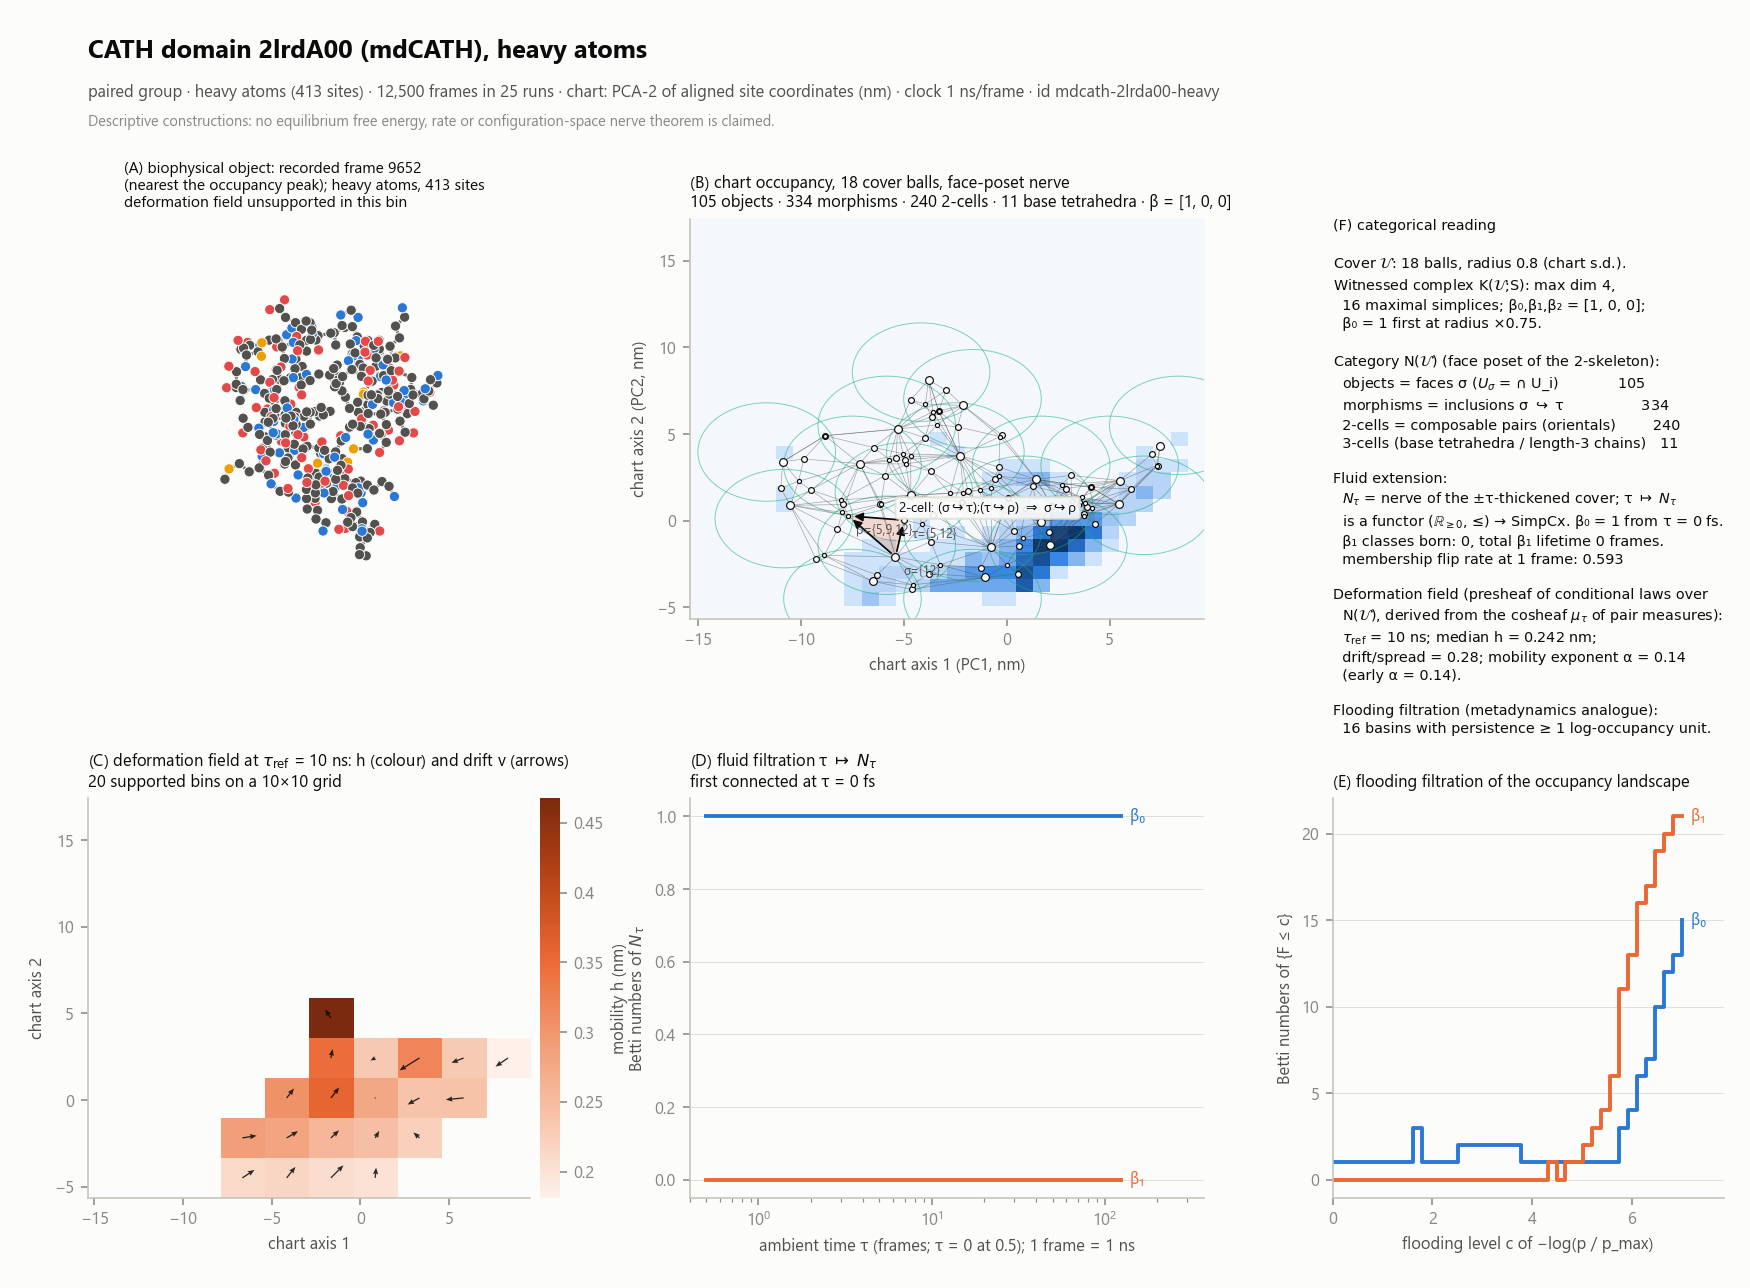
\includegraphics[width=\linewidth,height=.93\textheight,keepaspectratio]{systems/mdcath-2lrda00-heavy/plate.png}\caption{CATH domain 2lrdA00 (mdCATH), heavy atoms (\texttt{mdcath-2lrda00-heavy}), paired with \texttt{mdcath-2lrda00-ca}.}\end{figure}\clearpage
\begin{figure}[H]\centering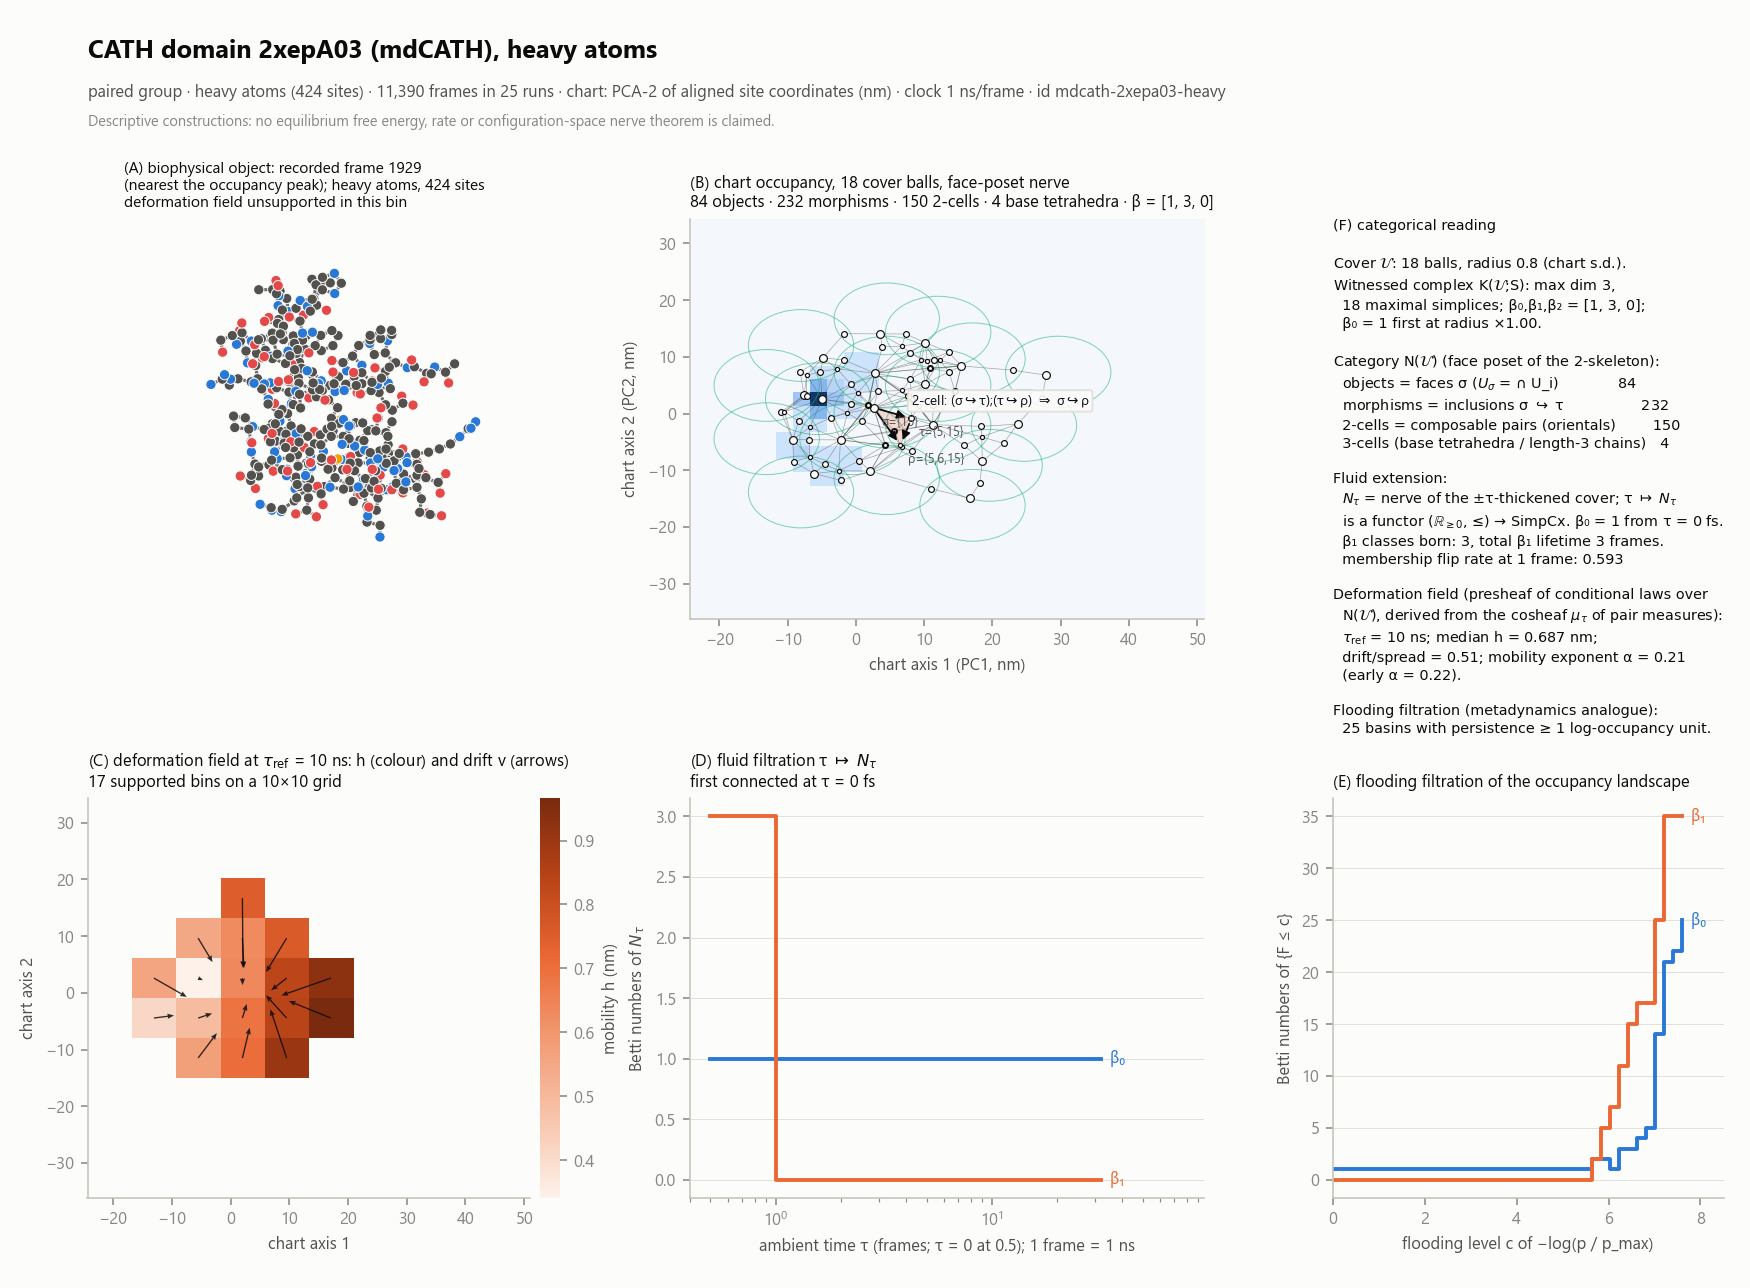
\includegraphics[width=\linewidth,height=.93\textheight,keepaspectratio]{systems/mdcath-2xepa03-heavy/plate.png}\caption{CATH domain 2xepA03 (mdCATH), heavy atoms (\texttt{mdcath-2xepa03-heavy}), paired with \texttt{mdcath-2xepa03-ca}.}\end{figure}\clearpage
\begin{figure}[H]\centering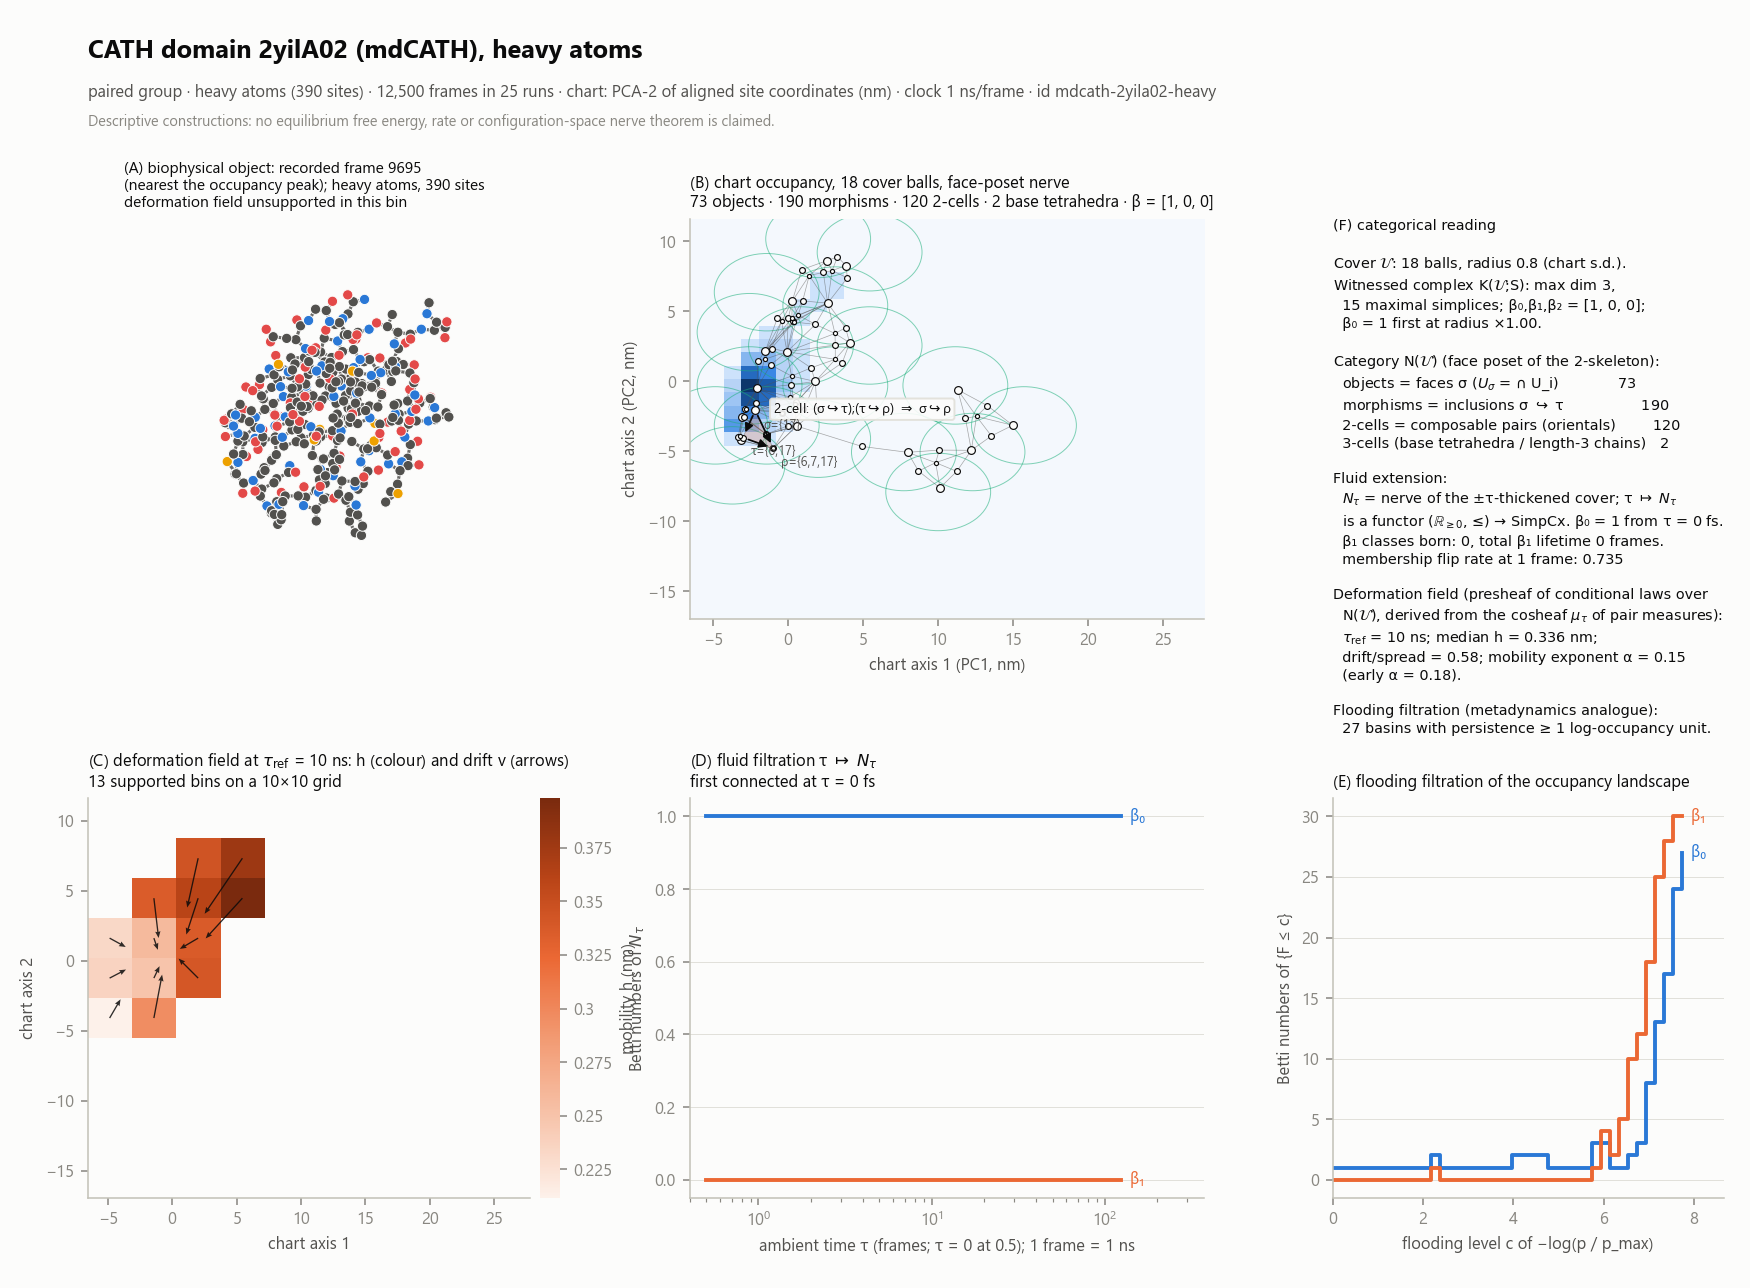
\includegraphics[width=\linewidth,height=.93\textheight,keepaspectratio]{systems/mdcath-2yila02-heavy/plate.png}\caption{CATH domain 2yilA02 (mdCATH), heavy atoms (\texttt{mdcath-2yila02-heavy}), paired with \texttt{mdcath-2yila02-ca}.}\end{figure}\clearpage
\begin{figure}[H]\centering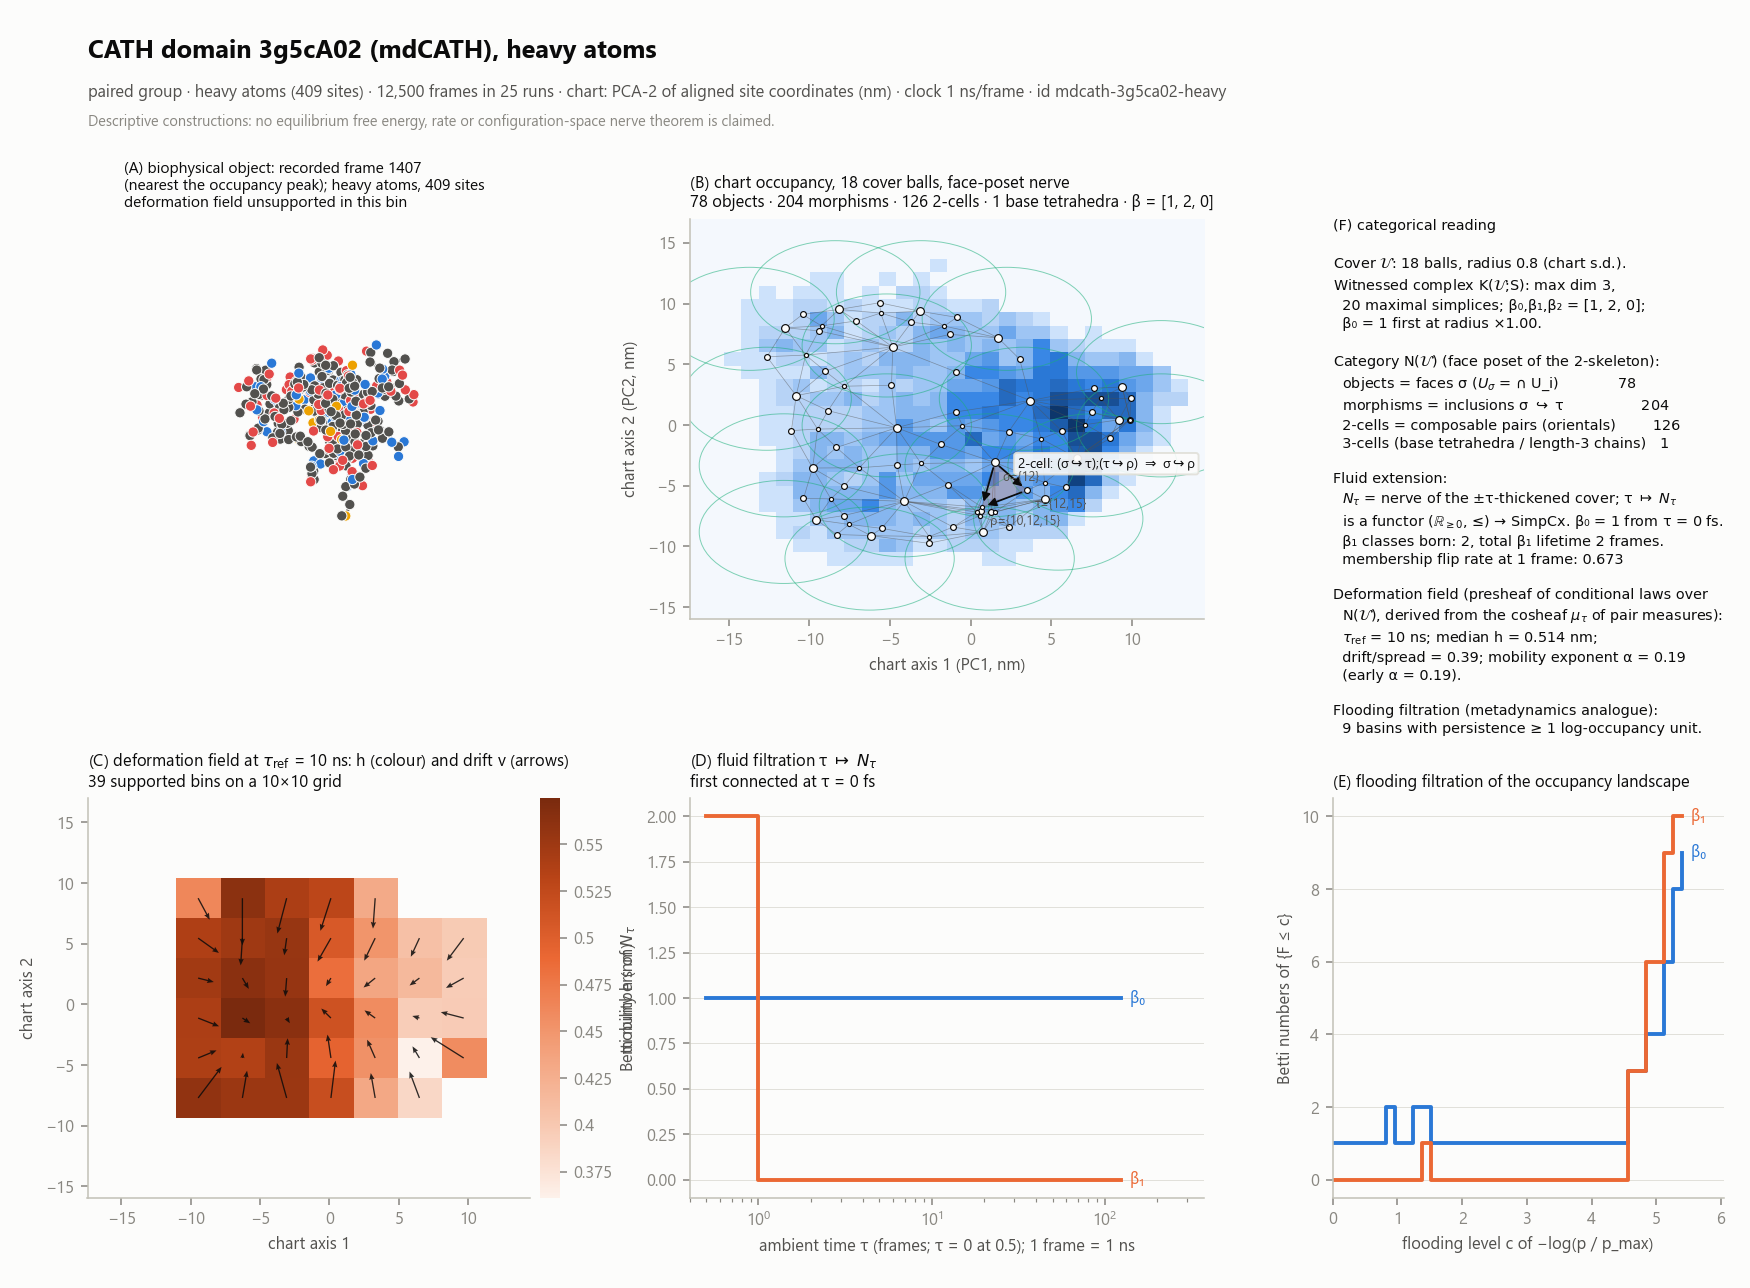
\includegraphics[width=\linewidth,height=.93\textheight,keepaspectratio]{systems/mdcath-3g5ca02-heavy/plate.png}\caption{CATH domain 3g5cA02 (mdCATH), heavy atoms (\texttt{mdcath-3g5ca02-heavy}), paired with \texttt{mdcath-3g5ca02-ca}.}\end{figure}\clearpage
\begin{figure}[H]\centering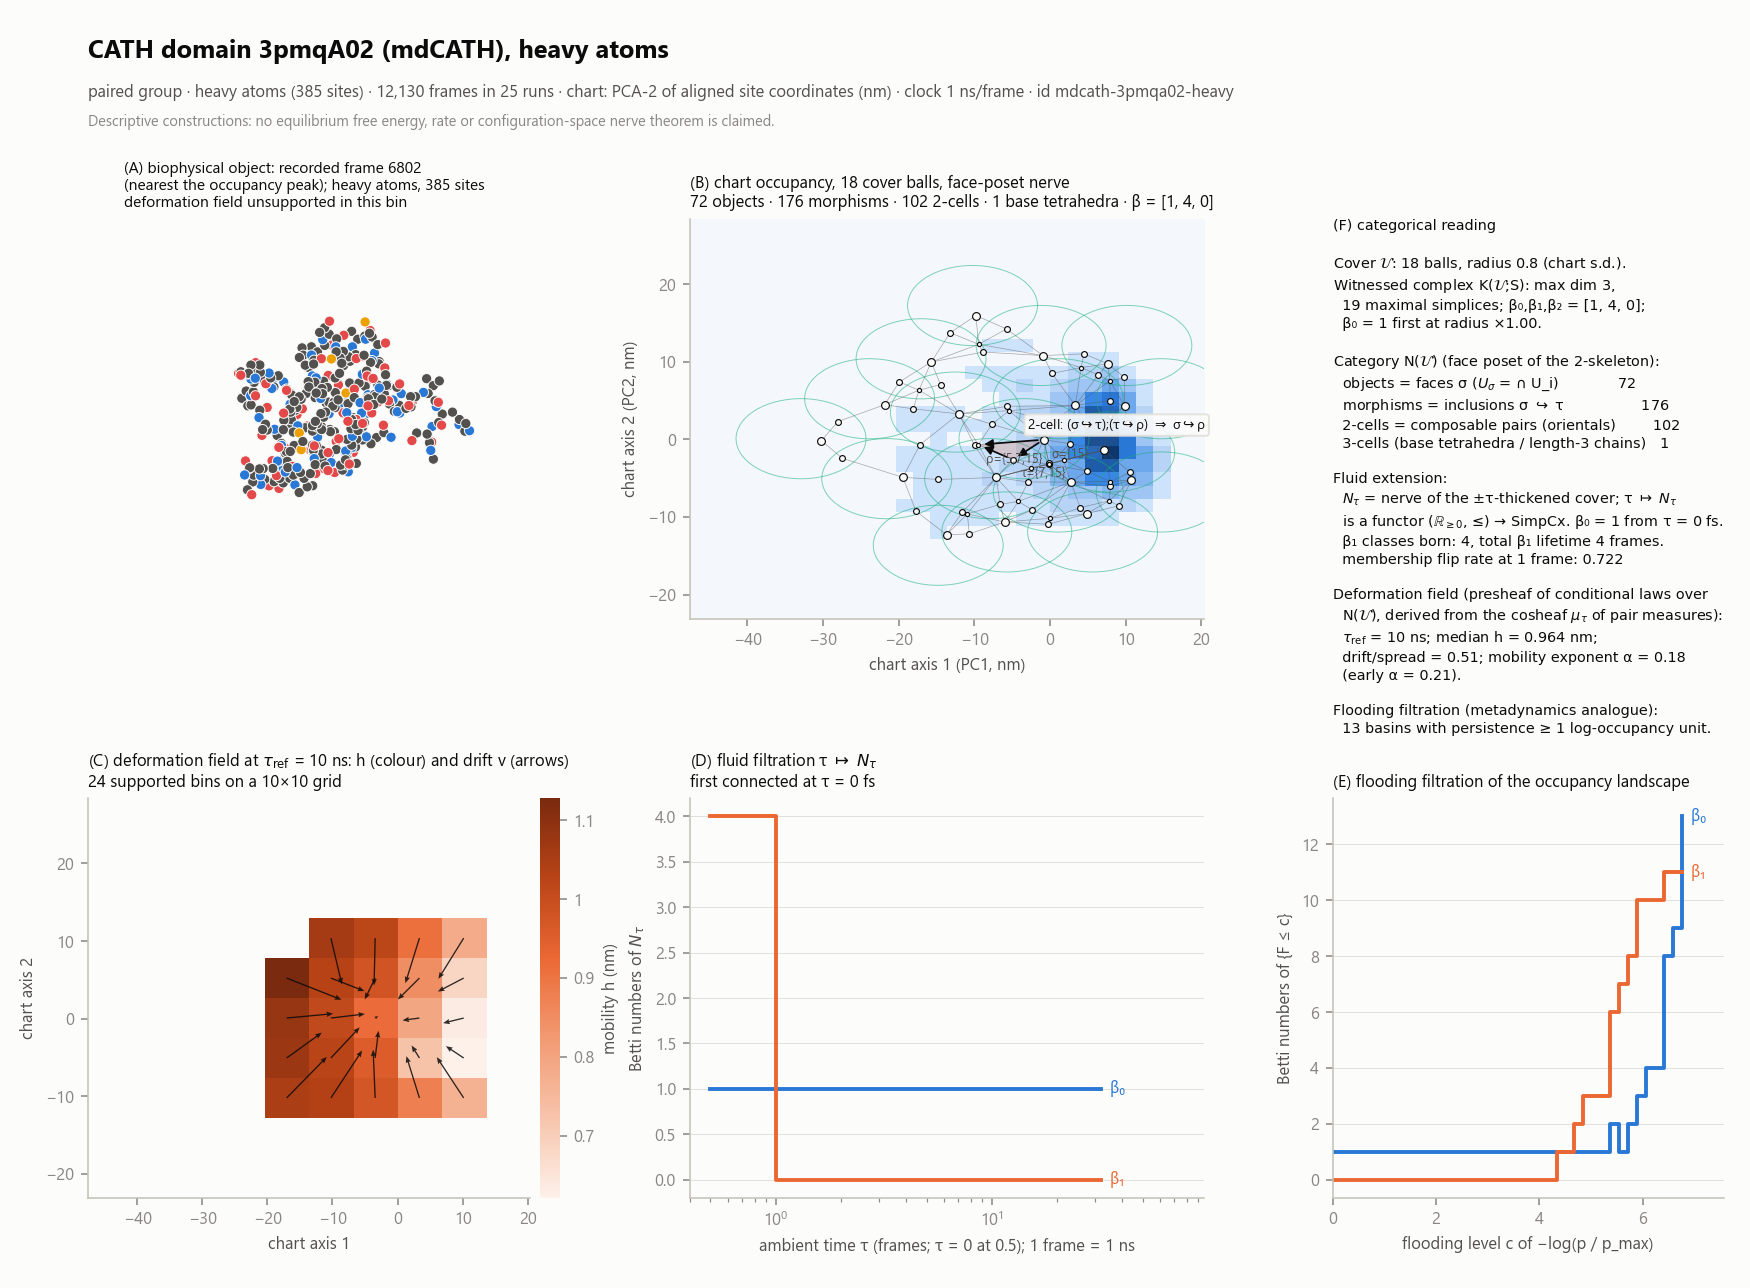
\includegraphics[width=\linewidth,height=.93\textheight,keepaspectratio]{systems/mdcath-3pmqa02-heavy/plate.png}\caption{CATH domain 3pmqA02 (mdCATH), heavy atoms (\texttt{mdcath-3pmqa02-heavy}), paired with \texttt{mdcath-3pmqa02-ca}.}\end{figure}\clearpage
\begin{figure}[H]\centering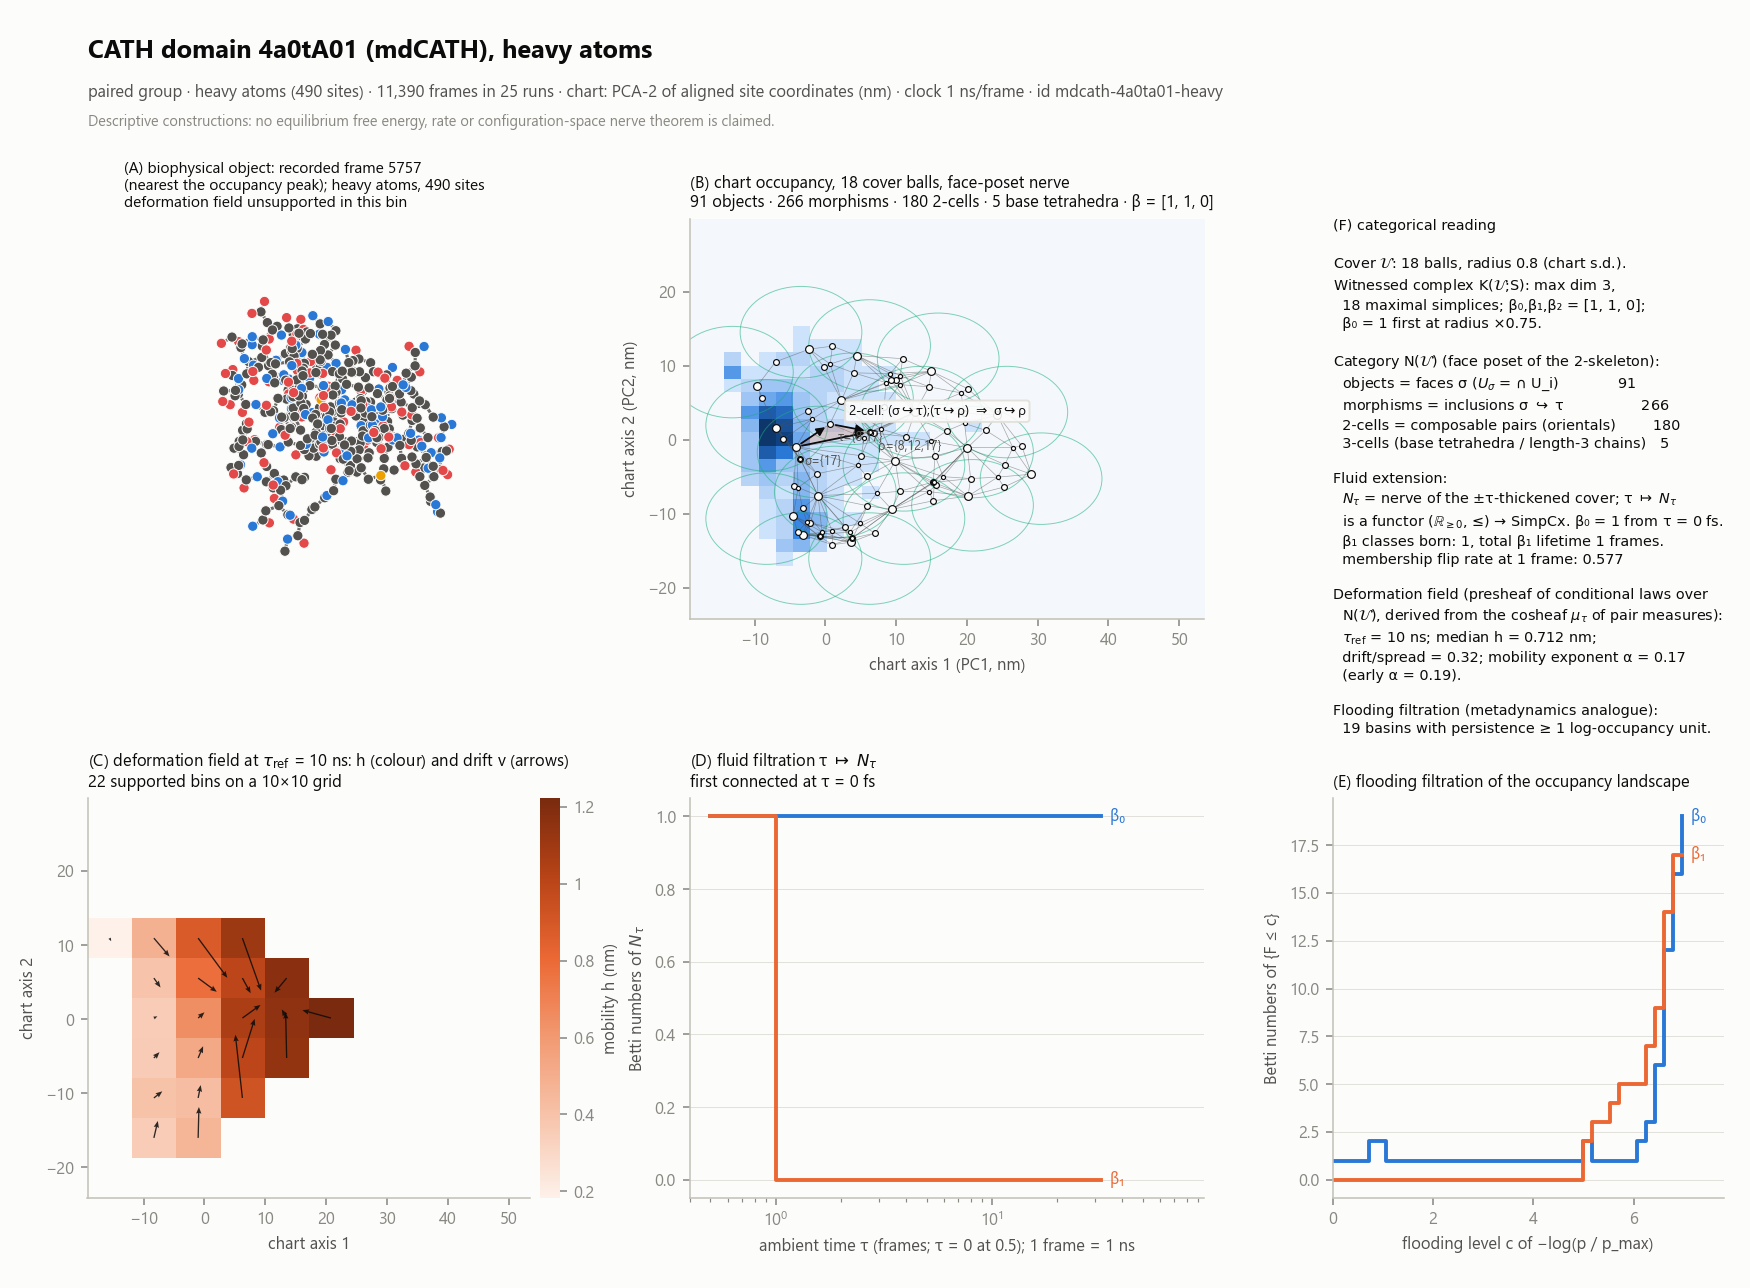
\includegraphics[width=\linewidth,height=.93\textheight,keepaspectratio]{systems/mdcath-4a0ta01-heavy/plate.png}\caption{CATH domain 4a0tA01 (mdCATH), heavy atoms (\texttt{mdcath-4a0ta01-heavy}), paired with \texttt{mdcath-4a0ta01-ca}.}\end{figure}\clearpage
\begin{figure}[H]\centering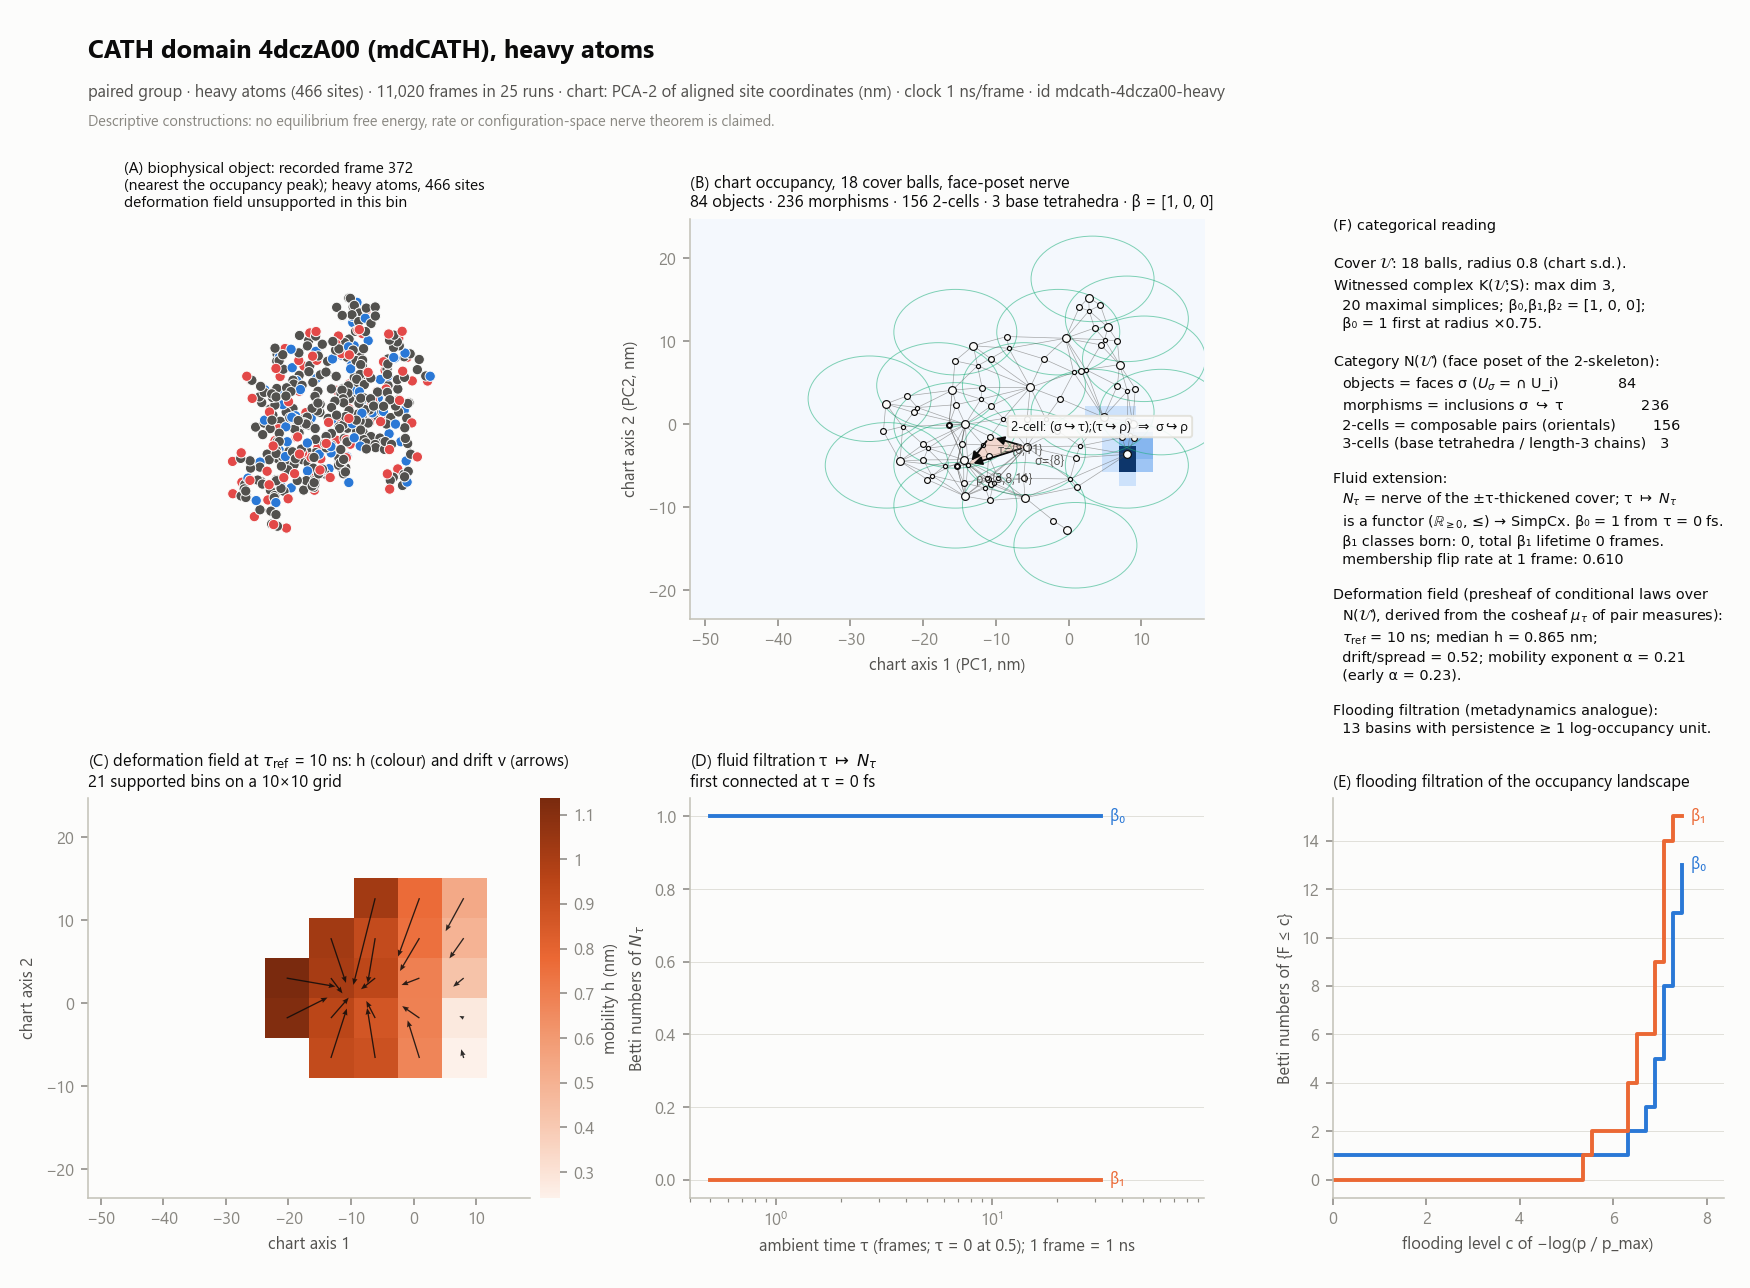
\includegraphics[width=\linewidth,height=.93\textheight,keepaspectratio]{systems/mdcath-4dcza00-heavy/plate.png}\caption{CATH domain 4dczA00 (mdCATH), heavy atoms (\texttt{mdcath-4dcza00-heavy}), paired with \texttt{mdcath-4dcza00-ca}.}\end{figure}\clearpage
\begin{figure}[H]\centering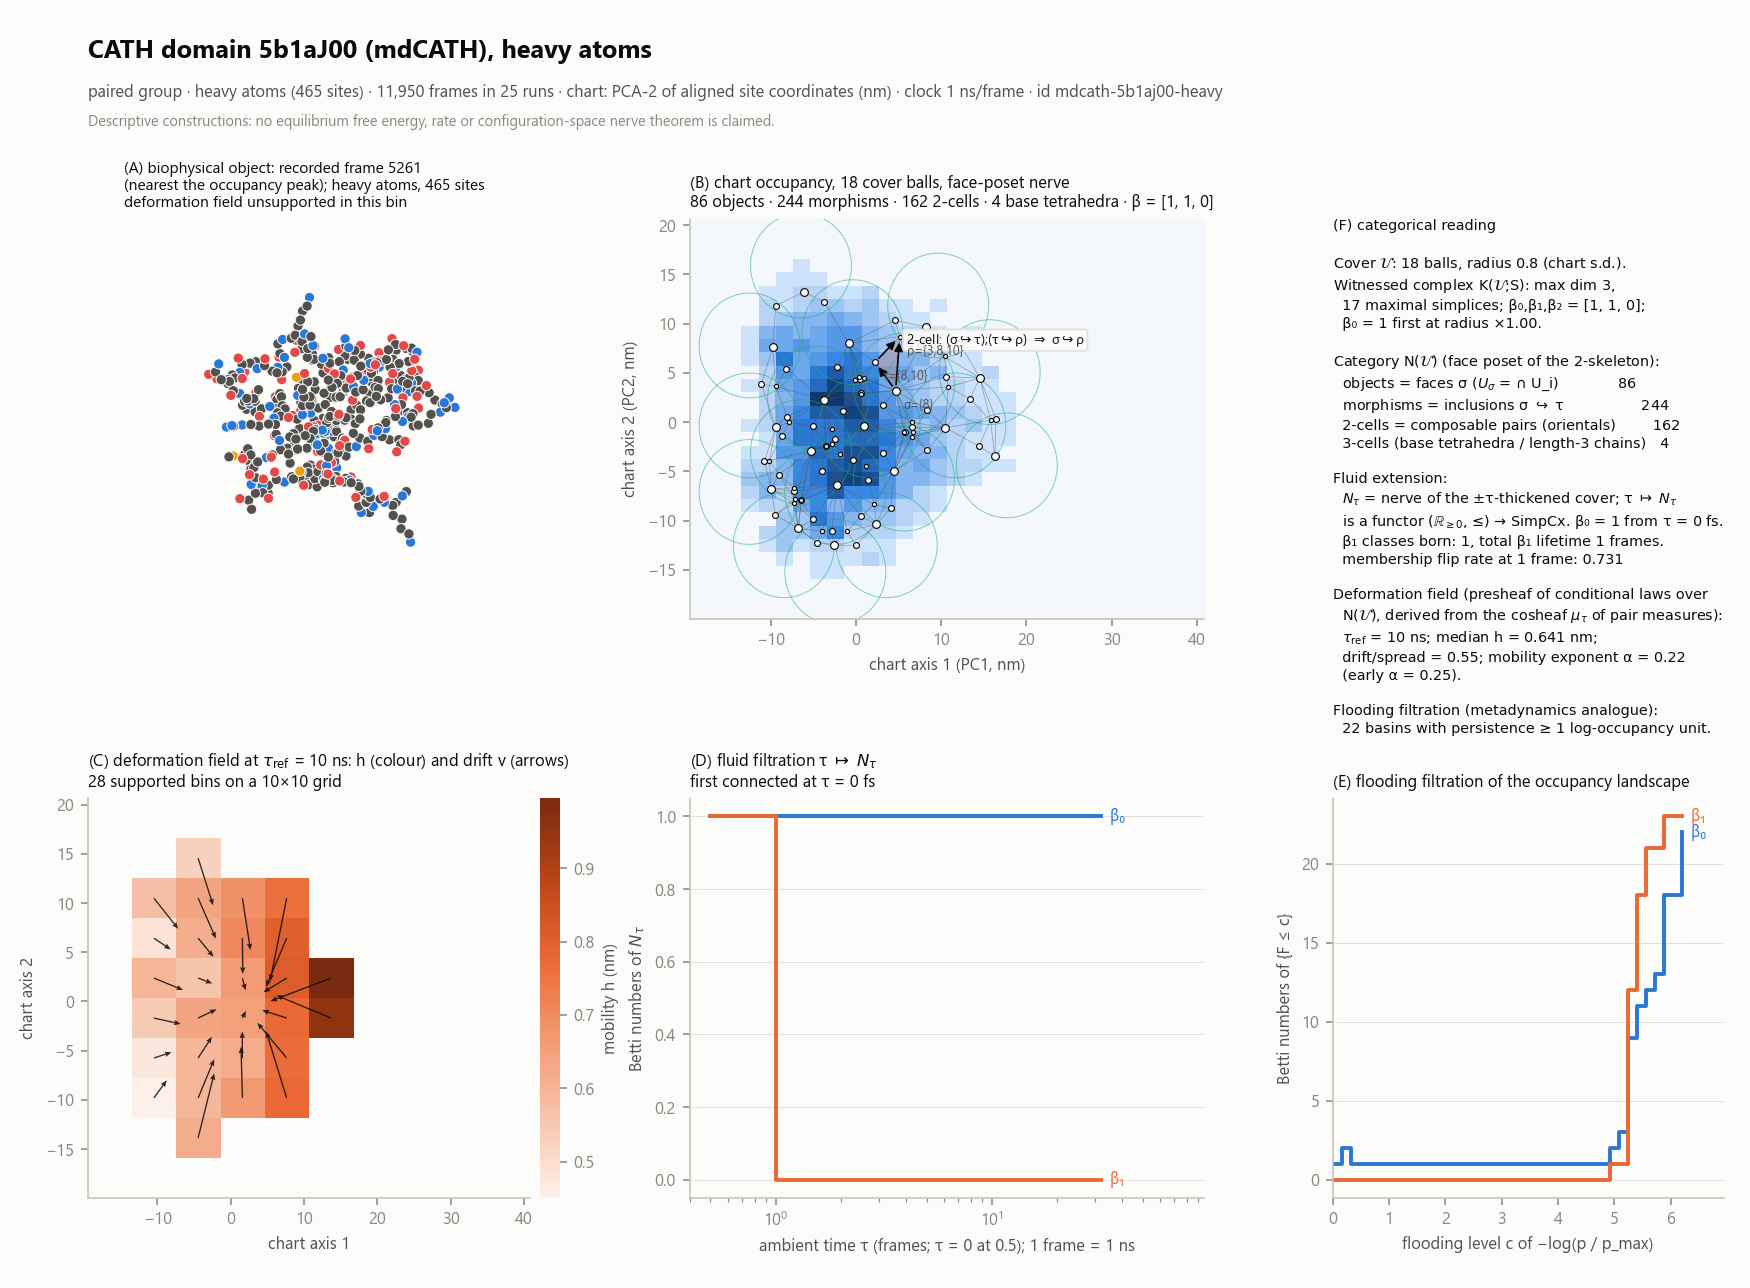
\includegraphics[width=\linewidth,height=.93\textheight,keepaspectratio]{systems/mdcath-5b1aj00-heavy/plate.png}\caption{CATH domain 5b1aJ00 (mdCATH), heavy atoms (\texttt{mdcath-5b1aj00-heavy}), paired with \texttt{mdcath-5b1aj00-ca}.}\end{figure}\clearpage
\begin{figure}[H]\centering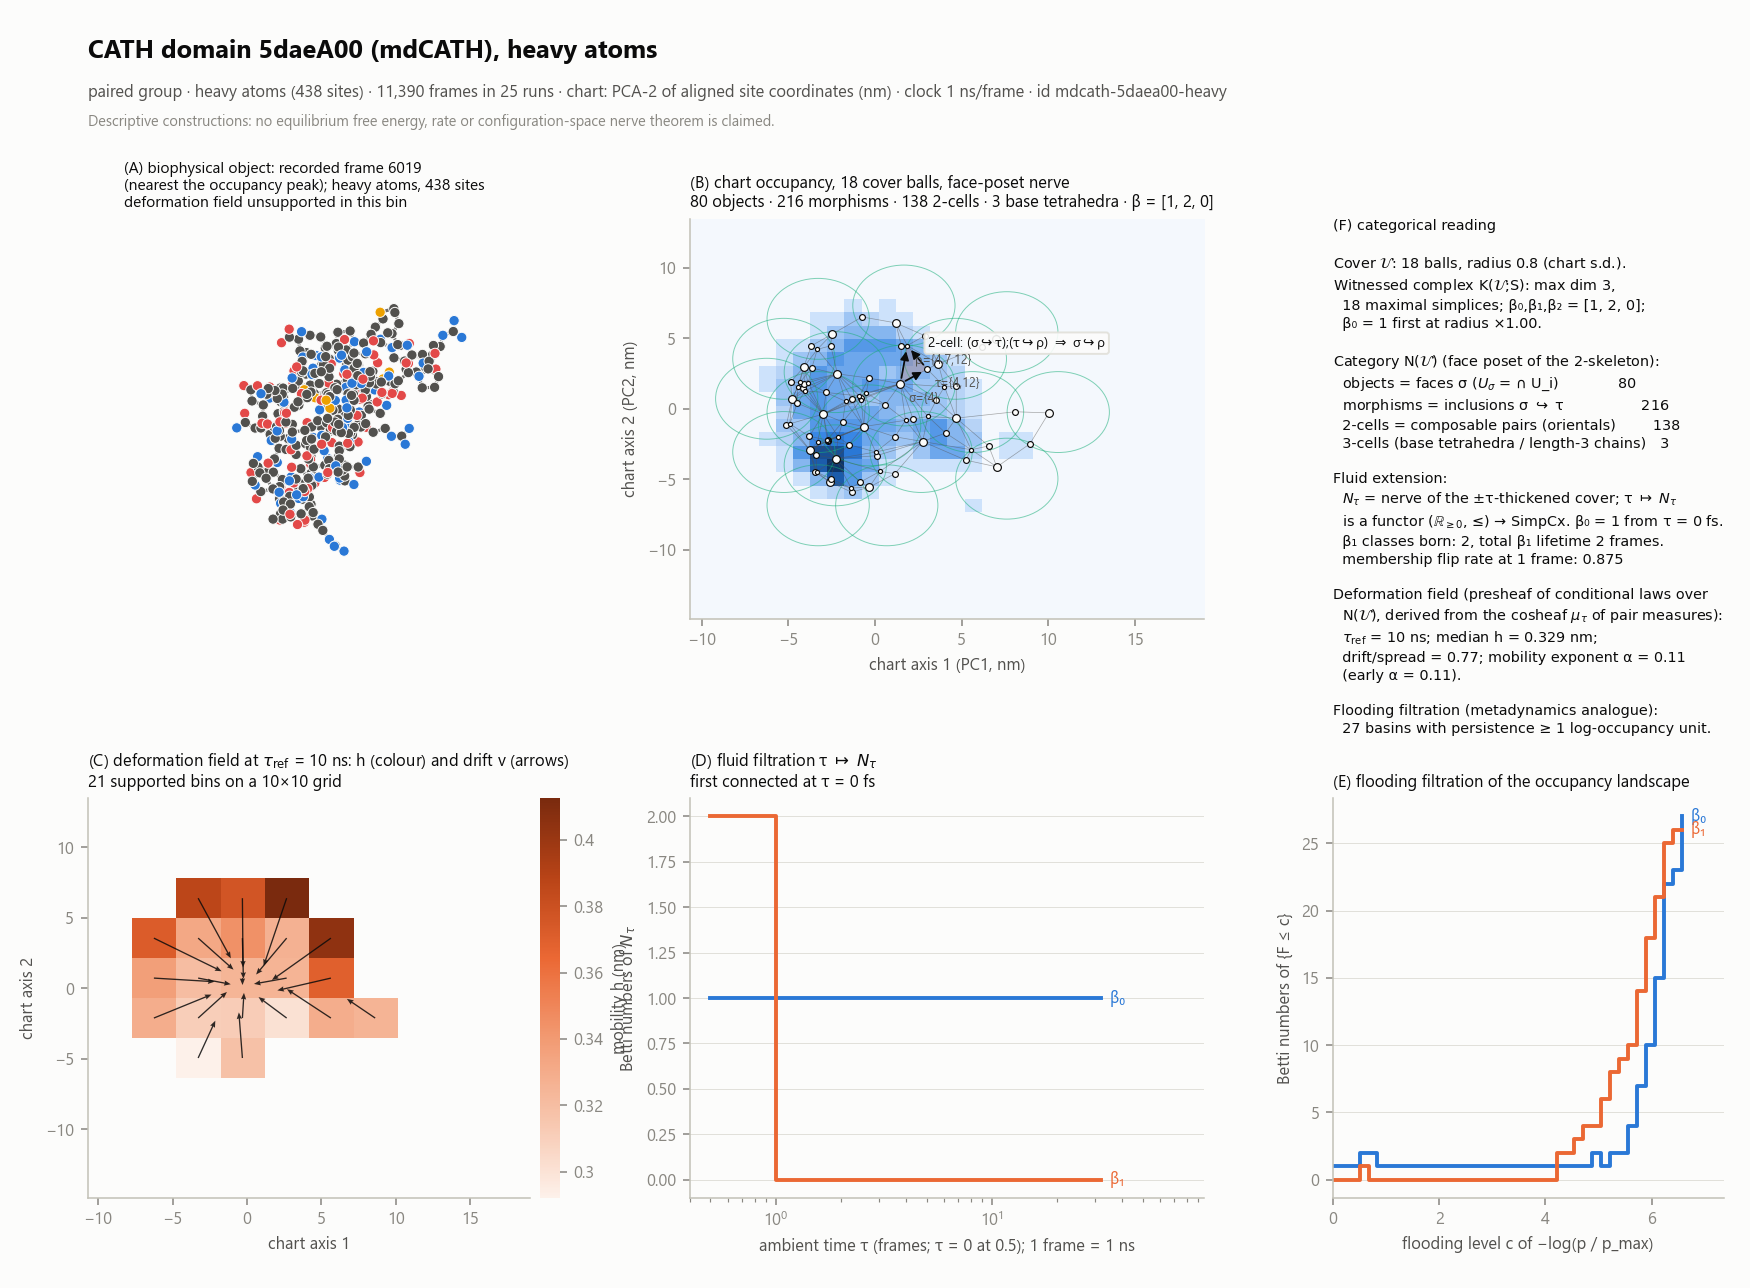
\includegraphics[width=\linewidth,height=.93\textheight,keepaspectratio]{systems/mdcath-5daea00-heavy/plate.png}\caption{CATH domain 5daeA00 (mdCATH), heavy atoms (\texttt{mdcath-5daea00-heavy}), paired with \texttt{mdcath-5daea00-ca}.}\end{figure}\clearpage
\end{document}